\selectlanguage{italian}

\chapter{\textit{Feature}}
Infine, il quinto capitolo ha come scopo quello di offrire un resoconto dell'\textit{output} dell'attività lavorativa personale, calando nella pratica i numerosi concetti più o meno teorici di cui si è discusso nelle precedenti sezioni. A tal fine, dopo una panoramica della procedura generale seguita ogni volta che è stato necessario realizzare un'implementazione, ovvero il “flusso di sviluppo standard”, sono state illustrate le più significative \textit{feature} sviluppate e implementate all'interno dell'applicativo.

Va sottolineato che le implementazioni qui riportate non sono tutte quelle realizzate nel corso dei mesi; per esigenze di spazio sono state descritte solamente quelle più rappresentative dei processi svolti e delle soluzioni adottate, realizzate nell'arco di tempo che va da agosto 2022 a dicembre 2022.

La convenzione adottata per la rappresentazione ordinata delle \textit{feature} include i seguenti elementi:
\begin{itemize}
    \item L'iniziale della parola \textit{feature} (“F”);
    \item Il numero progressivo;
    \item Il nome dell'implementazione.
\end{itemize}
% spazio
La loro disamina avviene secondo lo schema tripartito illustrato di seguito: 
\begin{enumerate}
    \item \textbf{Requisiti}: descrizione testuale di alto livello in cui vengono presentati i requisiti specifici richiesti committente;
    
    \item \textbf{Procedura}: descrizione, molto più precisa in termini di concetti e riferimenti, che accompagna e commenta al contempo il codice riportato;
    
    \item \textbf{\textit{Output} grafico}: \textit{screenshot} che mostrano il \textit{rendering} a schermo delle implementazioni effettuate.
\end{enumerate}
% spazio
Le \textit{feature} dotate di un notevole livello di similarità sono state accorpate in piccole sezioni tematiche. In questi casi, la descrizione della procedura e l'illustrazione dell'\textit{output} grafico è stata fornita solamente per la prima implementazione di quelle appartenenti a un gruppo.

\section{Flusso di sviluppo standard}
\label{sec:Flusso di sviluppo standard}
Attraverso l'espressione “flusso di sviluppo standard” si è deciso di rappresentare l'insieme ordinato e completo di tutti i passaggi seguiti nel corso dell'attività di sviluppo per la realizzazione di un'implementazione da un punto d'inizio zero.\\
Poiché tale flusso rappresenta uno scenario ideale e stereotipato, un \textit{template}, l'\textit{iter} realizzativo di ogni singola \textit{feature}, differente di volta in volta in termini di punto d'inizio e di fine e di passaggi eseguiti\footnote{Vari sono i fattori che determinano i punti d'inizio e di fine. Le richieste del committente e l'attività di sviluppo svolta in precedenza da altri membri del team costituiscono alcuni dei più influenti.}, può essere sempre contestualizzato all'interno di questa grande e onnicomprensiva procedura “padre”.

Lo schema riportato di seguito illustra sinteticamente la struttura del flusso di sviluppo standard.
\begin{enumerate}
    \item Posizionamento componente
        \begin{enumerate}
            \item \textit{Routing}
            \item \textit{Dashboard}
            \item \textit{Nesting}
        \end{enumerate}
    \item Funzioni di chiamata alle \gls{api} 
    \item Creazione componente
        \begin{enumerate}
            \item Logica
                \begin{enumerate}
                    \item Variabili di stato
                    \item Implementazione funzioni di chiamata alle \gls{api}
                    \item Schema
                \end{enumerate}
            \item \acrshort{ui}
        \end{enumerate}
\end{enumerate}


\newpage\section{F1 - F3: inserimento campo}
\label{sec:F1 - F3: inserimento campo}
Le \textit{feature} F1, F2 e F3 hanno previsto l'inserimento di un campo all'interno della tabella delle informazioni di un elemento, e l'aggiornamento della modale per l'aggiunta di un nuovo elemento, e per la modifica dei dati associati a un elemento esistente.
% Anche la procedura delle due \textit{feature} è sostanzialmente la stessa. Per questo motivo, se la descrizione dei passaggi seguiti è completa e meticolosa nel caso di F1, questa si limita alle differenze degne di nota nella discussione dell'implementazione di F2.
% Poiché la procedura è sostanzialmente identica in entrambi i casi la descrizione dettagliata dei passaggi eseguiti è stata effettuata solamente per F1.

\subsection{F1: visibilità nel sito web}
\label{subsec:F1: visibilità nel sito web}
\subparagraph{Requisiti}
La tabella che contiene le informazioni relative a una struttura medica deve essere dotata di un campo che riporti lo stato della visualizzazione (“Si” o “No”) sul sito web di Cerba HealthCare, nella pagina della struttura stessa.\\
La riga deve essere posta subito dopo il campo “Tipologia”.\\ 
Sia all'interno della modale per l'aggiunta di una nuova struttura medica che in quella di modifica dei dati di una struttura esistente, la gestione dello stato della visualizzazione sul sito web deve essere effettuata spuntando un \textit{flag}.

\subparagraph{Procedura}
Il \textbf{primo passo} compiuto è consistito nella creazione della logica responsabile del funzionamento delle porzioni di interfaccia da inserire.

Come illustrato nel \autoref{f1_ModalFacility_useState}, all'interno componente \texttt{ModalFacility} sono stati dichiarati la variabile di stato \texttt{website\_visibility} e il relativo \textit{setter} \texttt{setWebsiteVisibility()} tramite l'\textit{hook} \texttt{useState()}.\\
La variabile di stato è stata inizializzata (a riga 2) con una condizione che utilizza l'operatore ternario per esprimere il seguente concetto: se è vero che la proprietà \texttt{website\_visibility} dell'oggetto \texttt{facility} corrisponde\footnote{Più precisamente, l'operatore \textit{strict equality} (\texttt{===}) verifica che i due dati fra i quali è posto siano uguali sia per valore e che per tipo.} al valore booleano \texttt{true}, assegna il valore \texttt{true}, altrimenti \texttt{false}.

\lstinputlisting[caption=Variabile di stato \texttt{website\_visibility},  label=f1_ModalFacility_useState, language=JSX]{listings/capitolo5/f1_websiteVisibility/ModalFacility_useState.js}

Inoltre, è stato aggiornato il contenuto delle variabili \texttt{schema} e \texttt{form}\footnote{Generalmente, assieme a \texttt{schema} e \texttt{form} viene aggiornato anche l'oggetto \texttt{body}, ciò che viene passato all'\gls{api} innescata al click del bottone “Salva” della modale. In questo caso, ciò non è avvenuto a causa della struttura della variabile \texttt{body} stessa, che non ha necessitato dell'aggiunta della proprietà \texttt{website\_visibility}.} con l'aggiunta, in entrambi i casi, di una linea di codice relativa alla visibilità nel sito web.\\
Poiché la variabile \texttt{website\_visibility} opera con valori booleani, all'interno dell'oggetto \texttt{schema}, visibile nel \autoref{f1_ModalFacility_schema}, l'espressione \texttt{website\_visibility: yup.boolean()} (a riga 3) verifica che accada proprio questo.

\lstinputlisting[caption=Aggiornamento variabile \texttt{schema},label=f1_ModalFacility_schema, language=JSX]{listings/capitolo5/f1_websiteVisibility/ModalFacility_schema.js}
% spazio
L'oggetto \texttt{form}, visibile nel \autoref{f1_ModalFacility_form}, fa invece parte dell'\textit{handler} \texttt{handleSave()}\footnote{Attraverso le \textit{props}, la funzione \texttt{handleSave()} viene passata componente \texttt{ModalFacility} per essere utilizzata ogni volta che si clicca sul tasto salva.}, funzione che ha come compito il salvataggio dei dati una volta terminato il loro inserimento, lato client, nella modale. Tale oggetto vien passato come argomento alla funzione \texttt{validate()} per una validazione “generale” di quanto inserito nella finestra di dialogo; se i dati sono corretti viene eseguito il codice di \texttt{handleSave()} effettivamente responsabile del salvataggio dei dati\footnote{Il codice dell'\textit{handler} \texttt{handleSave()} che si occupa dell'effettivo salvataggio dei dati, qui non riportato, si avvale della sintassi \texttt{try...catch}. Per un esempio, si veda la \autoref{subsec:F6: “Magazine”}.}. L'aggiunta di \texttt{website\_visibility} (a riga 4) fra le proprietà dell'oggetto \texttt{form} va a segnalare che anche quest'ultima fa ora parte di quelle a lui appartenti.

\lstinputlisting[caption=Aggiornamento variabile \texttt{form},label=f1_ModalFacility_form, language=JSX]{listings/capitolo5/f1_websiteVisibility/ModalFacility_form.js}

Il \textbf{secondo passo}, illustrato nel \autoref{f1_ModalFacility_UI}, ha invece previsto due operazioni. Da un lato, è stata creata la porzione di \acrshort{ui} della modale atta alla gestione, lato client, dello stato relativo alla visualizzazione della struttura medica nel sito web. Il componente padre \texttt{Grid} \footnote{Il componente padre \texttt{Grid} e tutti i suoi figli (\texttt{Grid, Typography, FormGroup, FormControlLabel, <Checkbox}) sono a loro volta figli del componente \texttt{Dialog}.} (da riga 3 a 21) contiene al suo interno altri due componenti figli \texttt{Grid}, ognuno dei quali dotato, a sua volta, di un componente figlio. Rispettivamente, il primo \texttt{Grid} racchiude \texttt{Typography}, componente usato per la scrittura del nome della cella (“Visibilità”, a riga 5), mentre il secondo \texttt{FormGroup, FormControlLabel} e \texttt{Checkbox}, i componenti responsabili della struttura della \textit{checkbox} (da riga 9 a 20).\\
Dall'altro lato, la porzione di \acrshort{ui} appena descritta è stata dotata della logica discussa inizialmente. Le \textit{props} fornite al componente \texttt{Checkbox} sono \textit{props}:
\begin{itemize}
    \item \texttt{checked} (a riga 13): il suo valore è la variabile di stato \texttt{website\_visibility};
    
    \item \texttt{onChange} (a riga 14): il suo valore è una funzione che, sfruttando il funzionamento del \textit{setter} \texttt{setWebsiteVisibiliy()}, ha il compito di sostituire il precedente valore della variabile di stato \texttt{website\_visibility}.
\end{itemize}
Queste linee di codice concludono le modifiche alla modale per l'aggiunta di una nuova struttura medica e per la modifica dei dati di una struttura esistente visualizzati nella relativa tabella delle informazioni.

\lstinputlisting[caption=\textit{Checkbox} modifica visibilità sito web, label=f1_ModalFacility_UI, language=JSX]{listings/capitolo5/f1_websiteVisibility/ModalFacility_UI.js}

Il \textbf{terzo} e \textbf{ultimo passo} compiuto, quello che segna la chiusura del processo nella sua interezza, ha riguardato l'aggiornamento della \acrshort{ui} della tabella delle informazioni (della struttura medica, fra cui anche lo stato della visualizzazione sul sito web), alla quale è stata poi fornita la logica per il funzionamento. Tutto ciò è stato svolto all'interno del componente \texttt{TabInfo} ed è illustrato nel \autoref{f1_TabInfo_UI}.

Il componente \texttt{TableRow} (da riga 3 a 6) rappresenta sia la nuova riga aggiunta alla tabella già esistente\footnote{Il componente \texttt{TableRow} e i suoi figli (\texttt{TableCell}) sono a loro volta figli del componente \texttt{Table}.}, che un elemento padre. I suoi due componenti figli altro non sono che le celle della riga in cui saranno presentate le informazioni:
\begin{itemize}
    \item \texttt{TableCell} (a riga 4): contiene il nome della riga appena aggiunta, “Visibilità sul sito web”;
    
    \item \texttt{TableCell} (a riga 5): contiene una condizione che utilizza l'operatore terniario per esprimere il seguente concetto: se è vero che il valore della proprietà \texttt{website\_visibility} dell'oggetto \texttt{facility} è \texttt{true} assegna come la valore la stringa \texttt{"Si"}, altrimenti la stringa \texttt{"No"}.
\end{itemize}

\lstinputlisting[caption=Riga visibilità sito web, label=f1_TabInfo_UI, language=JSX]{listings/capitolo5/f1_websiteVisibility/TabInfo_UI.js}

\subsection{F2: e-mail}
\subparagraph{Requisiti}
La tabella che contiene le informazioni relative alla singola struttura medica deve essere dotata di una nuovo campo che riporti la sua e-mail.\\
La riga deve essere posta fra i campi “Brand storico” e “Telefono”.\\ 
All'interno della modale di modifica dei dati di una struttura esistente, il campo di testo dell'e-mail deve presentare l'e-mail qualora essa sia presente ed essere vuoto in caso contrario; invece, all'interno della modale di aggiunta di una nuova struttura, il campo di testo dell'e-mail deve semplicemente essere vuoto.

% \subparagraph{Procedura}
% Come anticipato nella \autoref{sec:F1 - F3: inserimento campo}, la descrizione del processo realizzativo della \textit{feature} F2 è circoscritta ai soli aspetti dotati di un adeguato carattere di diversità rispetto a quelli già trattati a proposito di F1.

% L'inizializzazione della variabile di stato \texttt{e-mail} avviene tramite un'espressione che esprime il seguente concetto: se la proprietà \texttt{email} (contenuta dall'oggetto \texttt{facility}) è vera (esiste, ha un contenuto), il suo valore sarà la variabile \texttt{e-mail} stessa, altrimenti una stringa vuota \texttt{""}. Ciò è illustrato nel \autoref{f2_ModalFacility_useState}.

% \lstinputlisting[caption=Variabile di stato \texttt{e-mail}, label=f2_ModalFacility_useState, language=JSX]{listings/capitolo5/f2_email/ModalFacility_useState.js}

% % ! rivedere
% L'aggiornamento della variabile \texttt{schema}, invece visibile nel \autoref{f2_ModalFacility_schema}. Questo ha previsto l'aggiunta della proprietà \texttt{email} (a riga 3) e \texttt{yup.string()} come suo valore, per verificare che la variabile operi solamente con valori di tipo stringa. Ulteriori vincoli sul valore di \texttt{email} sono stabiliti del metodo \texttt{matches()}; il suo compito, da un lato è di verificare che la proprietà rispetti le convenzioni previste per le e-mail, e dall'altro di restituire un messaggio di errore. 

% \lstinputlisting[caption=Aggiornamento della variabile \texttt{schema}, label=f2_ModalFacility_schema, language=JSX]{listings/capitolo5/f2_email/ModalFacility_schema.js}

% \lstinputlisting[caption=Aggiornamento delle variabile \texttt{form},label=f2_ModalFacility_form, language=JSX]{listings/capitolo5/f2_email/ModalFacility_form.js}

% Il \autoref{f2_ModalFacility_UI} mostra la porzione di UI della modale per la gestione del campo \texttt{e-mail}. Come illustrato da riga 8 a 15, la sua creazione ha previsto l'utilizzo del componente \texttt{TextField}; fra le sue \textit{props}, sia \texttt{label} che \texttt{placeholder} hanno come valore la stringa \texttt{"E-mail"}, mentre \texttt{value} ha la variabile di stato \texttt{e-mail} precedentemente dichiarata.\\
% % ! rivedere
% Il discorso si complica rispetto all'espressione riportata a riga 12 (???).

% \lstinputlisting[caption=\textit{TextField} per la modifica del campo e-mail, label=f2_ModalFacility_UI, language=JSX]{listings/capitolo5/f2_email/ModalFacility_UI.js}

% Come riportato a riga 5 del \autoref{f2_TabInfo_UI}, il contenuto del componente \texttt{TableCell} è la proprietà \texttt{email} (contenuta dall'oggetto \texttt{facility}).

% \lstinputlisting[caption=Riga rappresentante l'e-mail, label=f2_TabInfo_UI, language=JSX]{listings/capitolo5/f2_email/TabInfo_UI.js}

\subsection{F3: link referti e portale prenotazione}
\subparagraph{Requisiti}
La tabella che contiene le informazioni relative alla singola struttura medica deve essere dotata di una nuovo campo che riporti il link per l'inserimento dei referti.\\
La riga deve essere posta in coda ai campi esistenti.\\ 
All'interno della modale, il campo di testo del link dei referti deve presentare il link, qualora esso sia presente e si sia in fase di modifica dei dati di una struttura esistente, o essere vuoto, qualora esso sia assente e si sia in fase di aggiunta di una nuova struttura.

La tabella che contiene le informazioni relative alla singola \textit{business unit} (BU) deve essere dotata di due nuovi campi, uno che riporti il link del portale di prenotazione, e uno che riporti il link del portale di prenotazione SSN.\\
All'interno della modale, il campo di testo di entrambi i link deve presentare il link, qualora esso sia presente e si sia in fase di modifica dei dati di una struttura esistente, o essere vuoto, qualora esso sia assente e si sia in fase di aggiunta di una nuova struttura.

\newpage\paragraph{\textit{Output} grafico}
% \begin{figure}[H]
%     \centering
%     \subfloat[][\emph{Modale aggiunta parte 1}]
%         {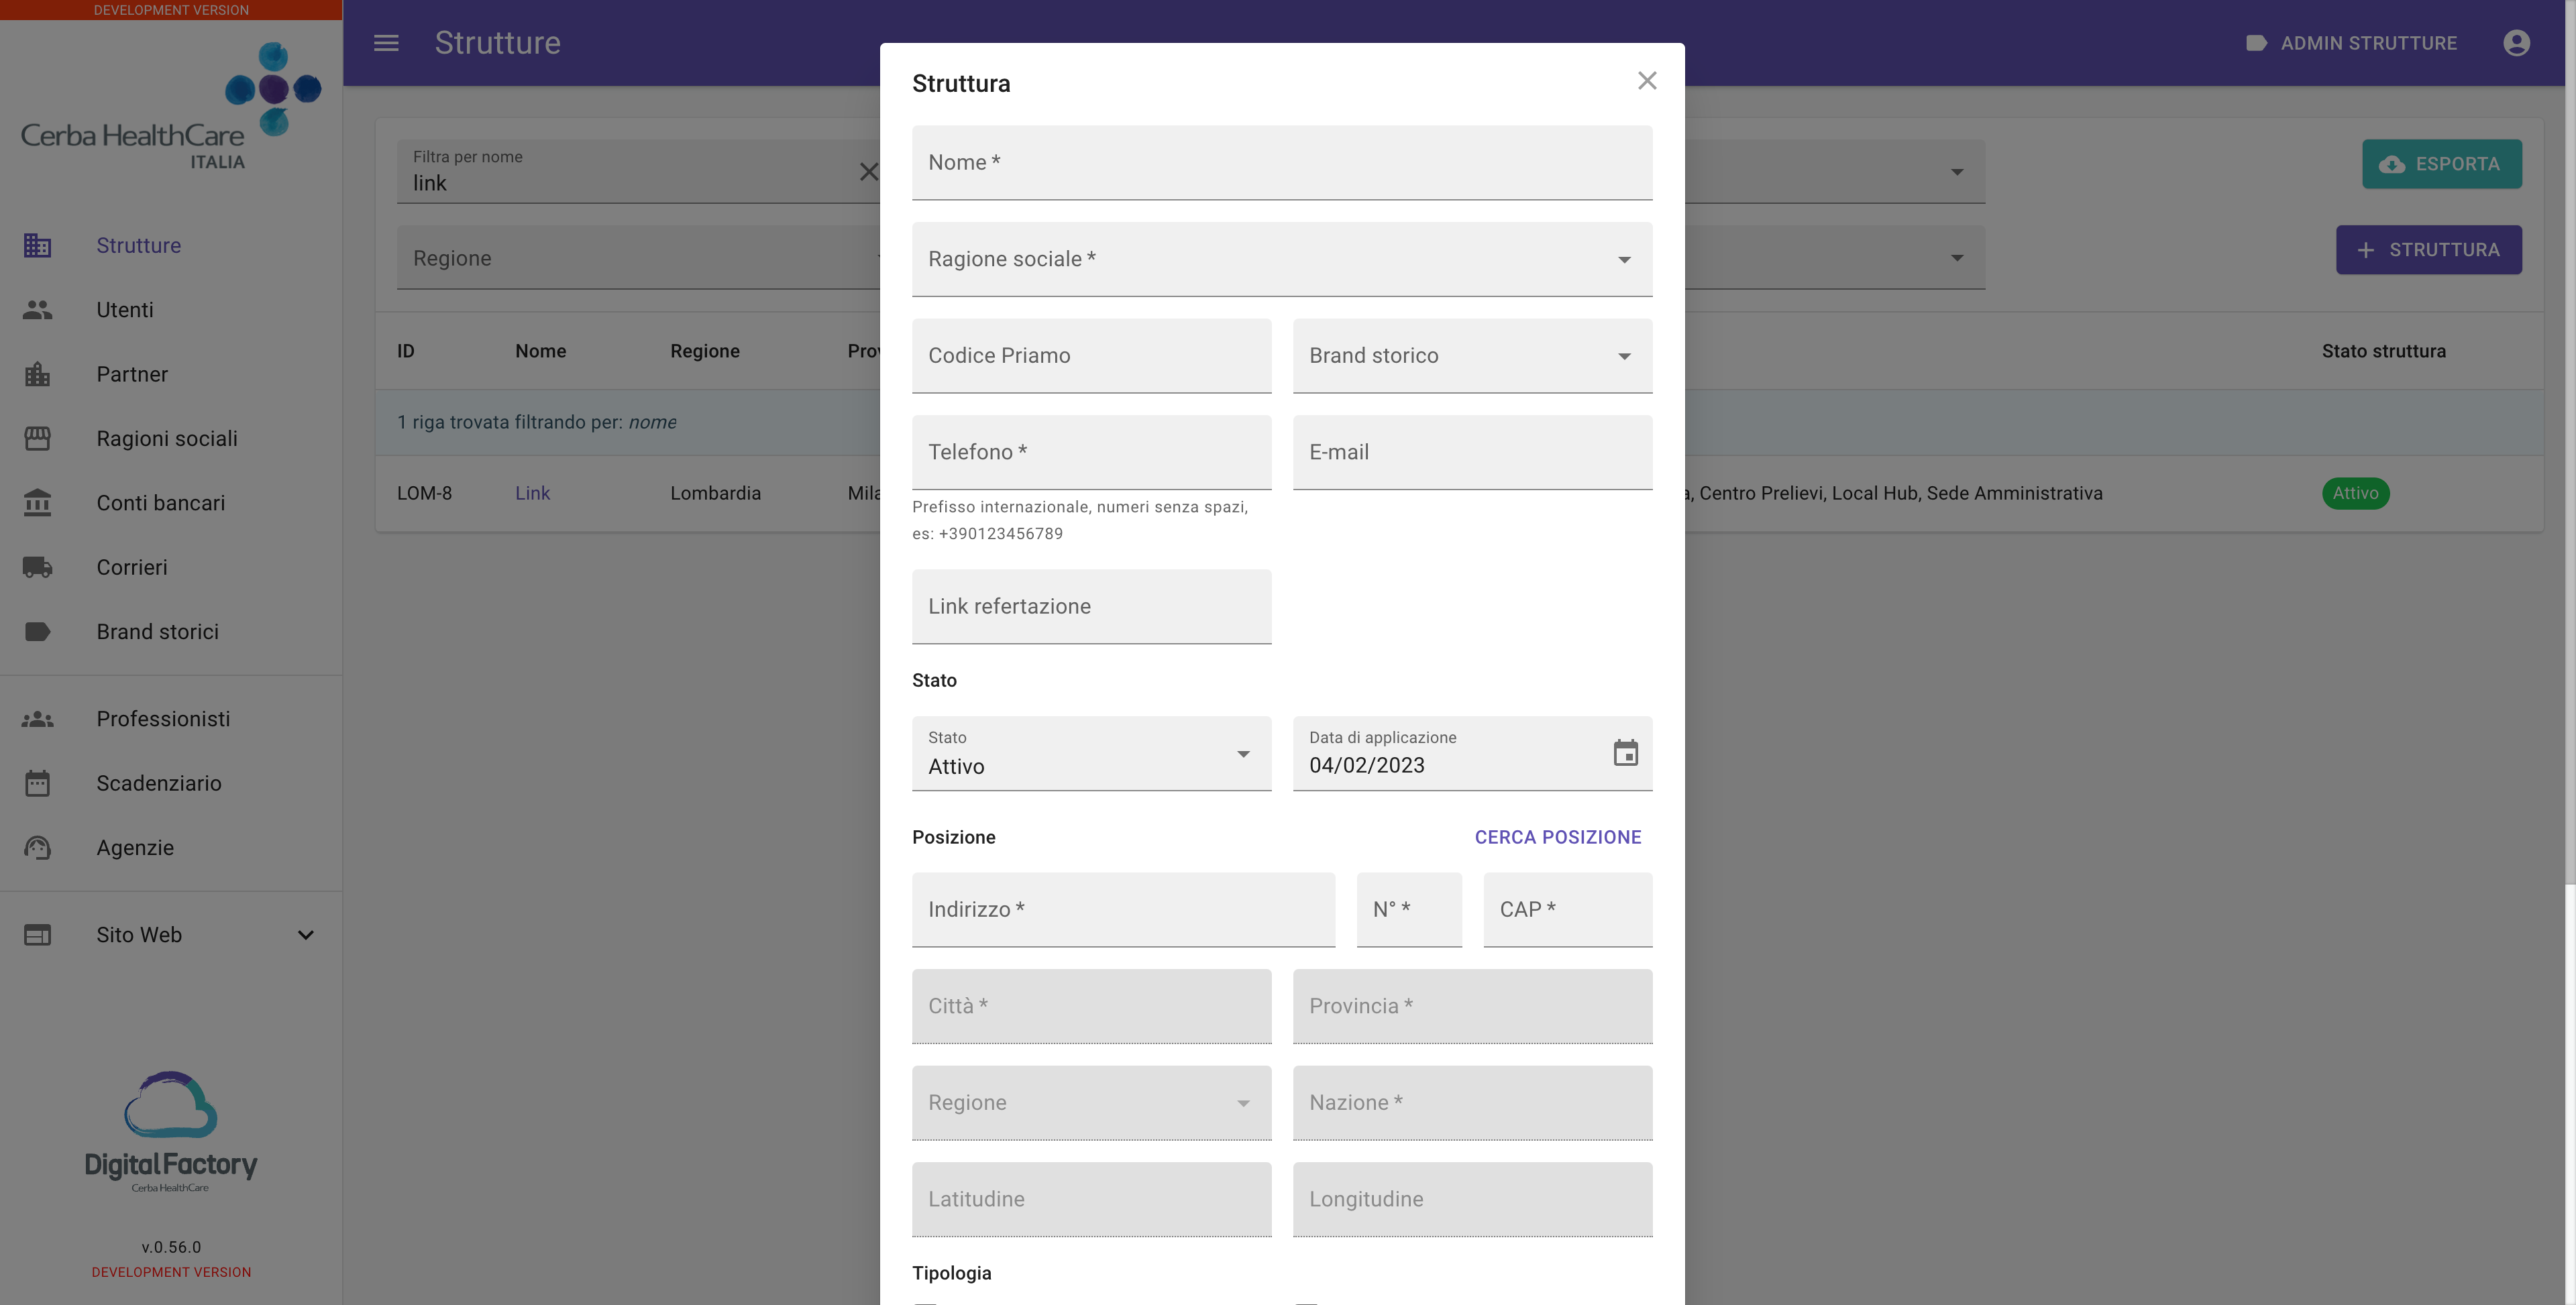
\includegraphics[width= 0.48\textwidth]{images/capitolo5/f1_f2_f3_websiteVisibility_email_links/ModalFacility_create_pt1.png}} \quad
%     \subfloat[][\emph{Modale aggiunta parte 2}]
%         {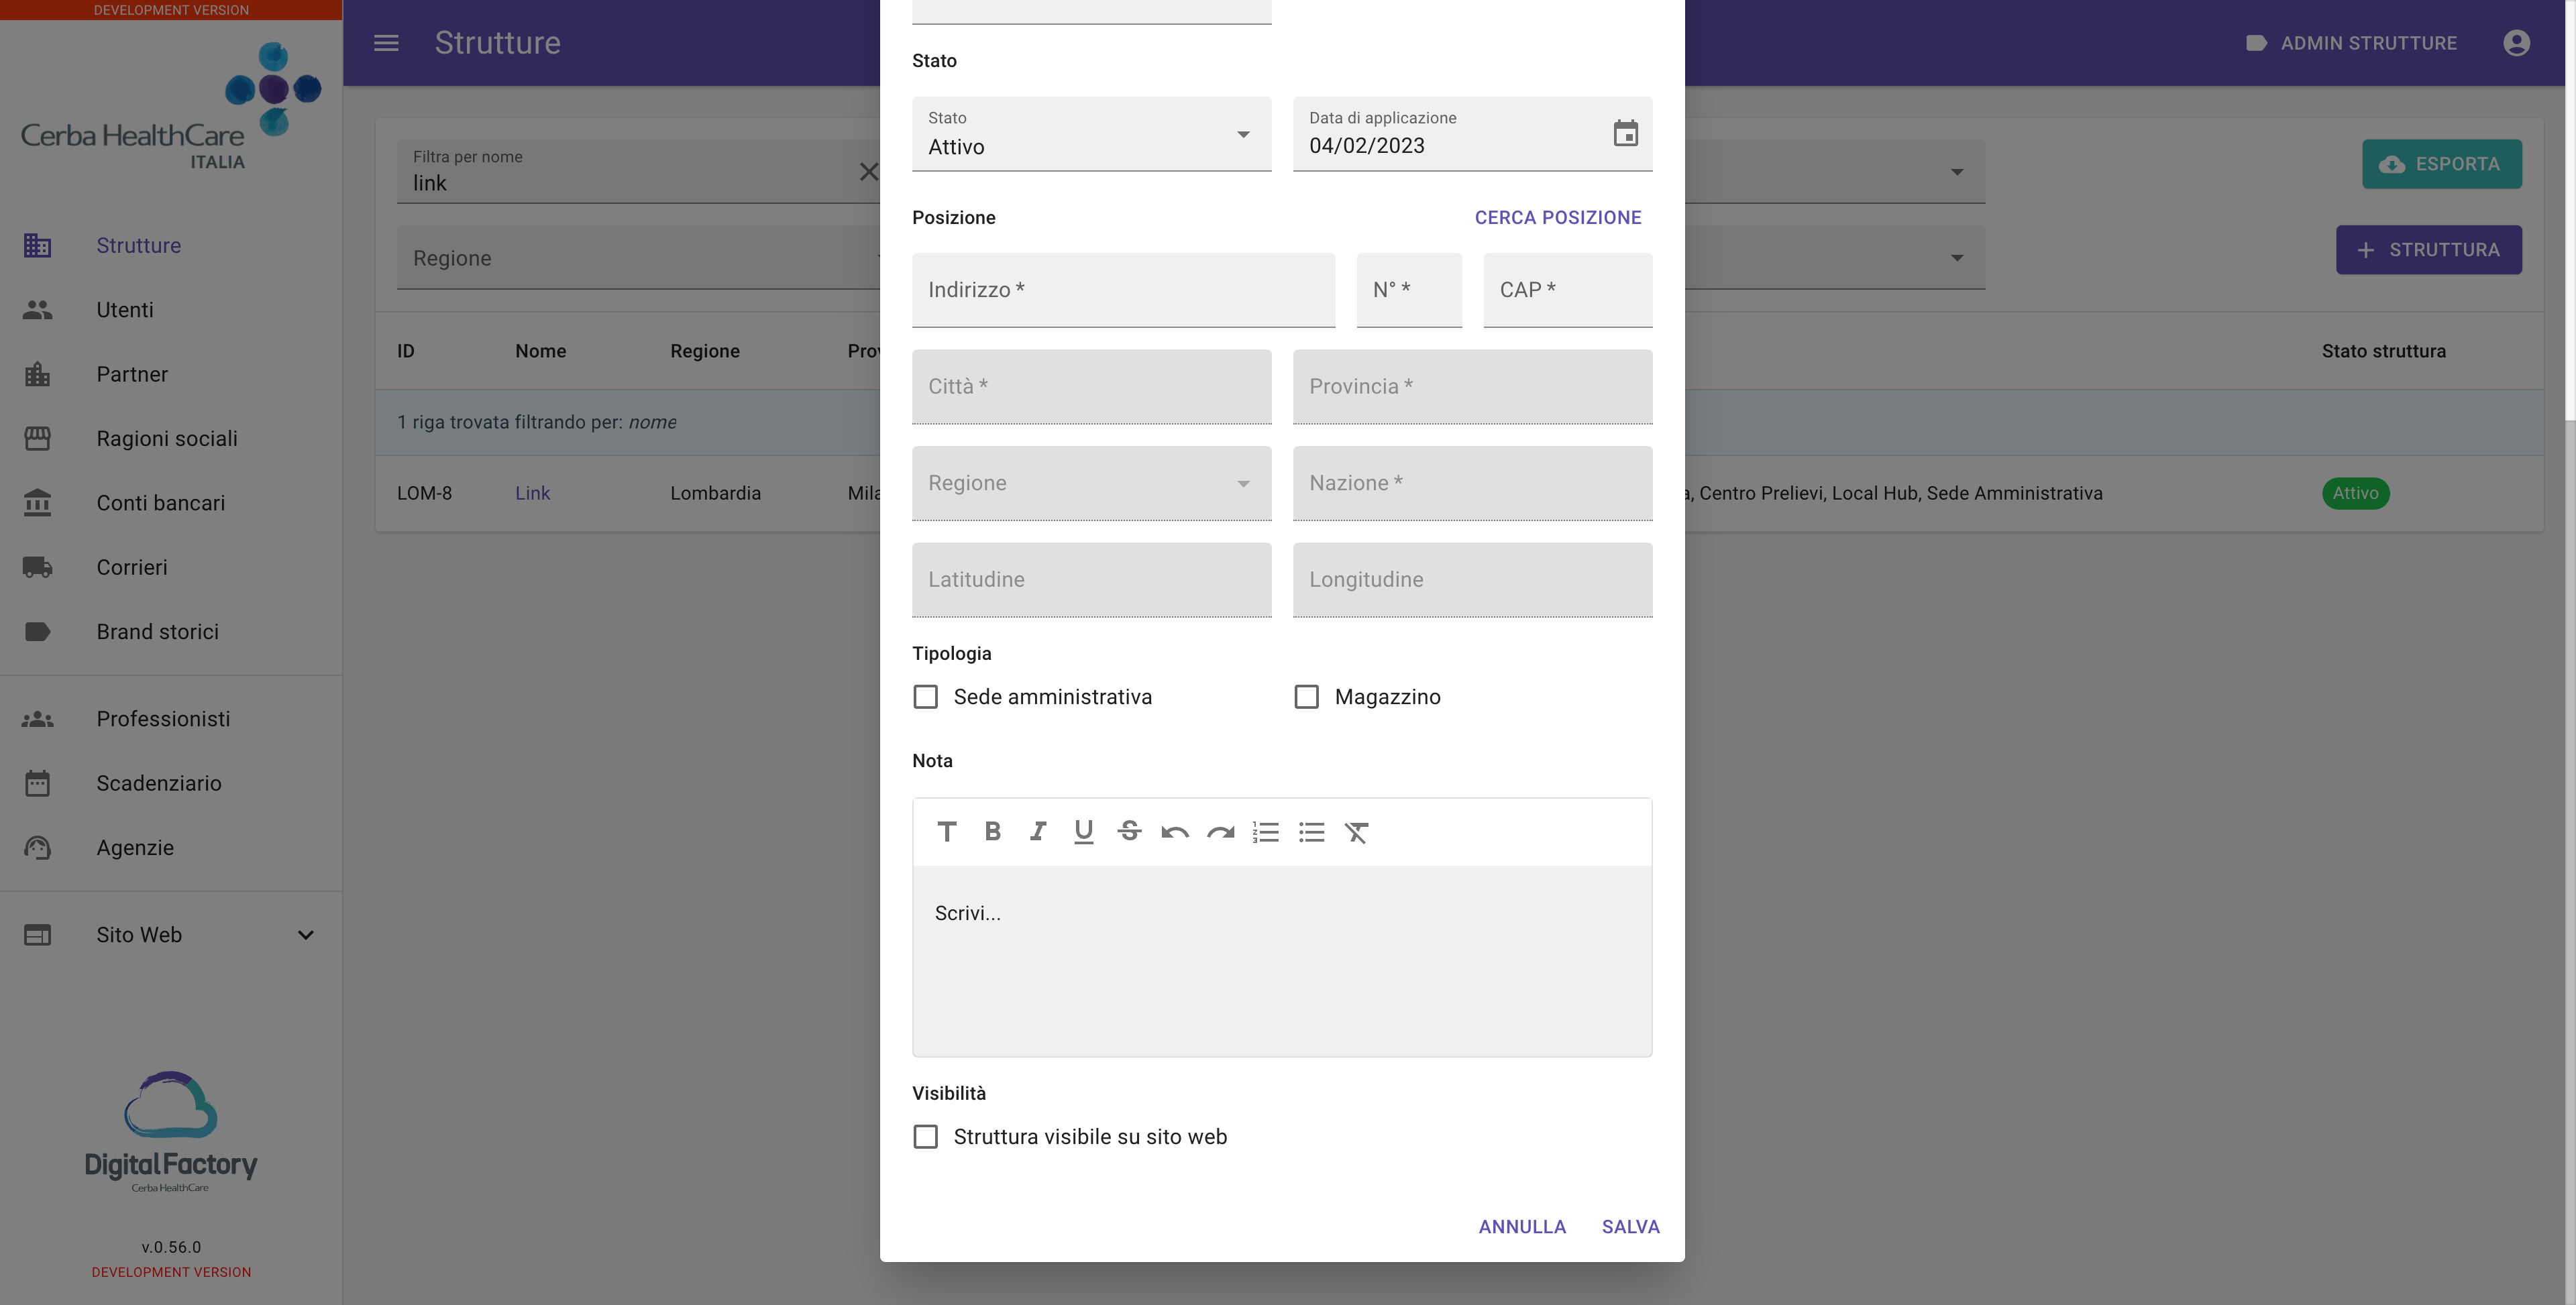
\includegraphics[width= 0.48\textwidth]{images/capitolo5/f1_f2_f3_websiteVisibility_email_links/ModalFacility_create_pt2.png}} 
%     \caption{Modale aggiunta nuova struttura}
%     % \label{fig:Modale aggiunta nuova struttura}    
% \end{figure}

% \begin{figure}[H]
%     \centering
%     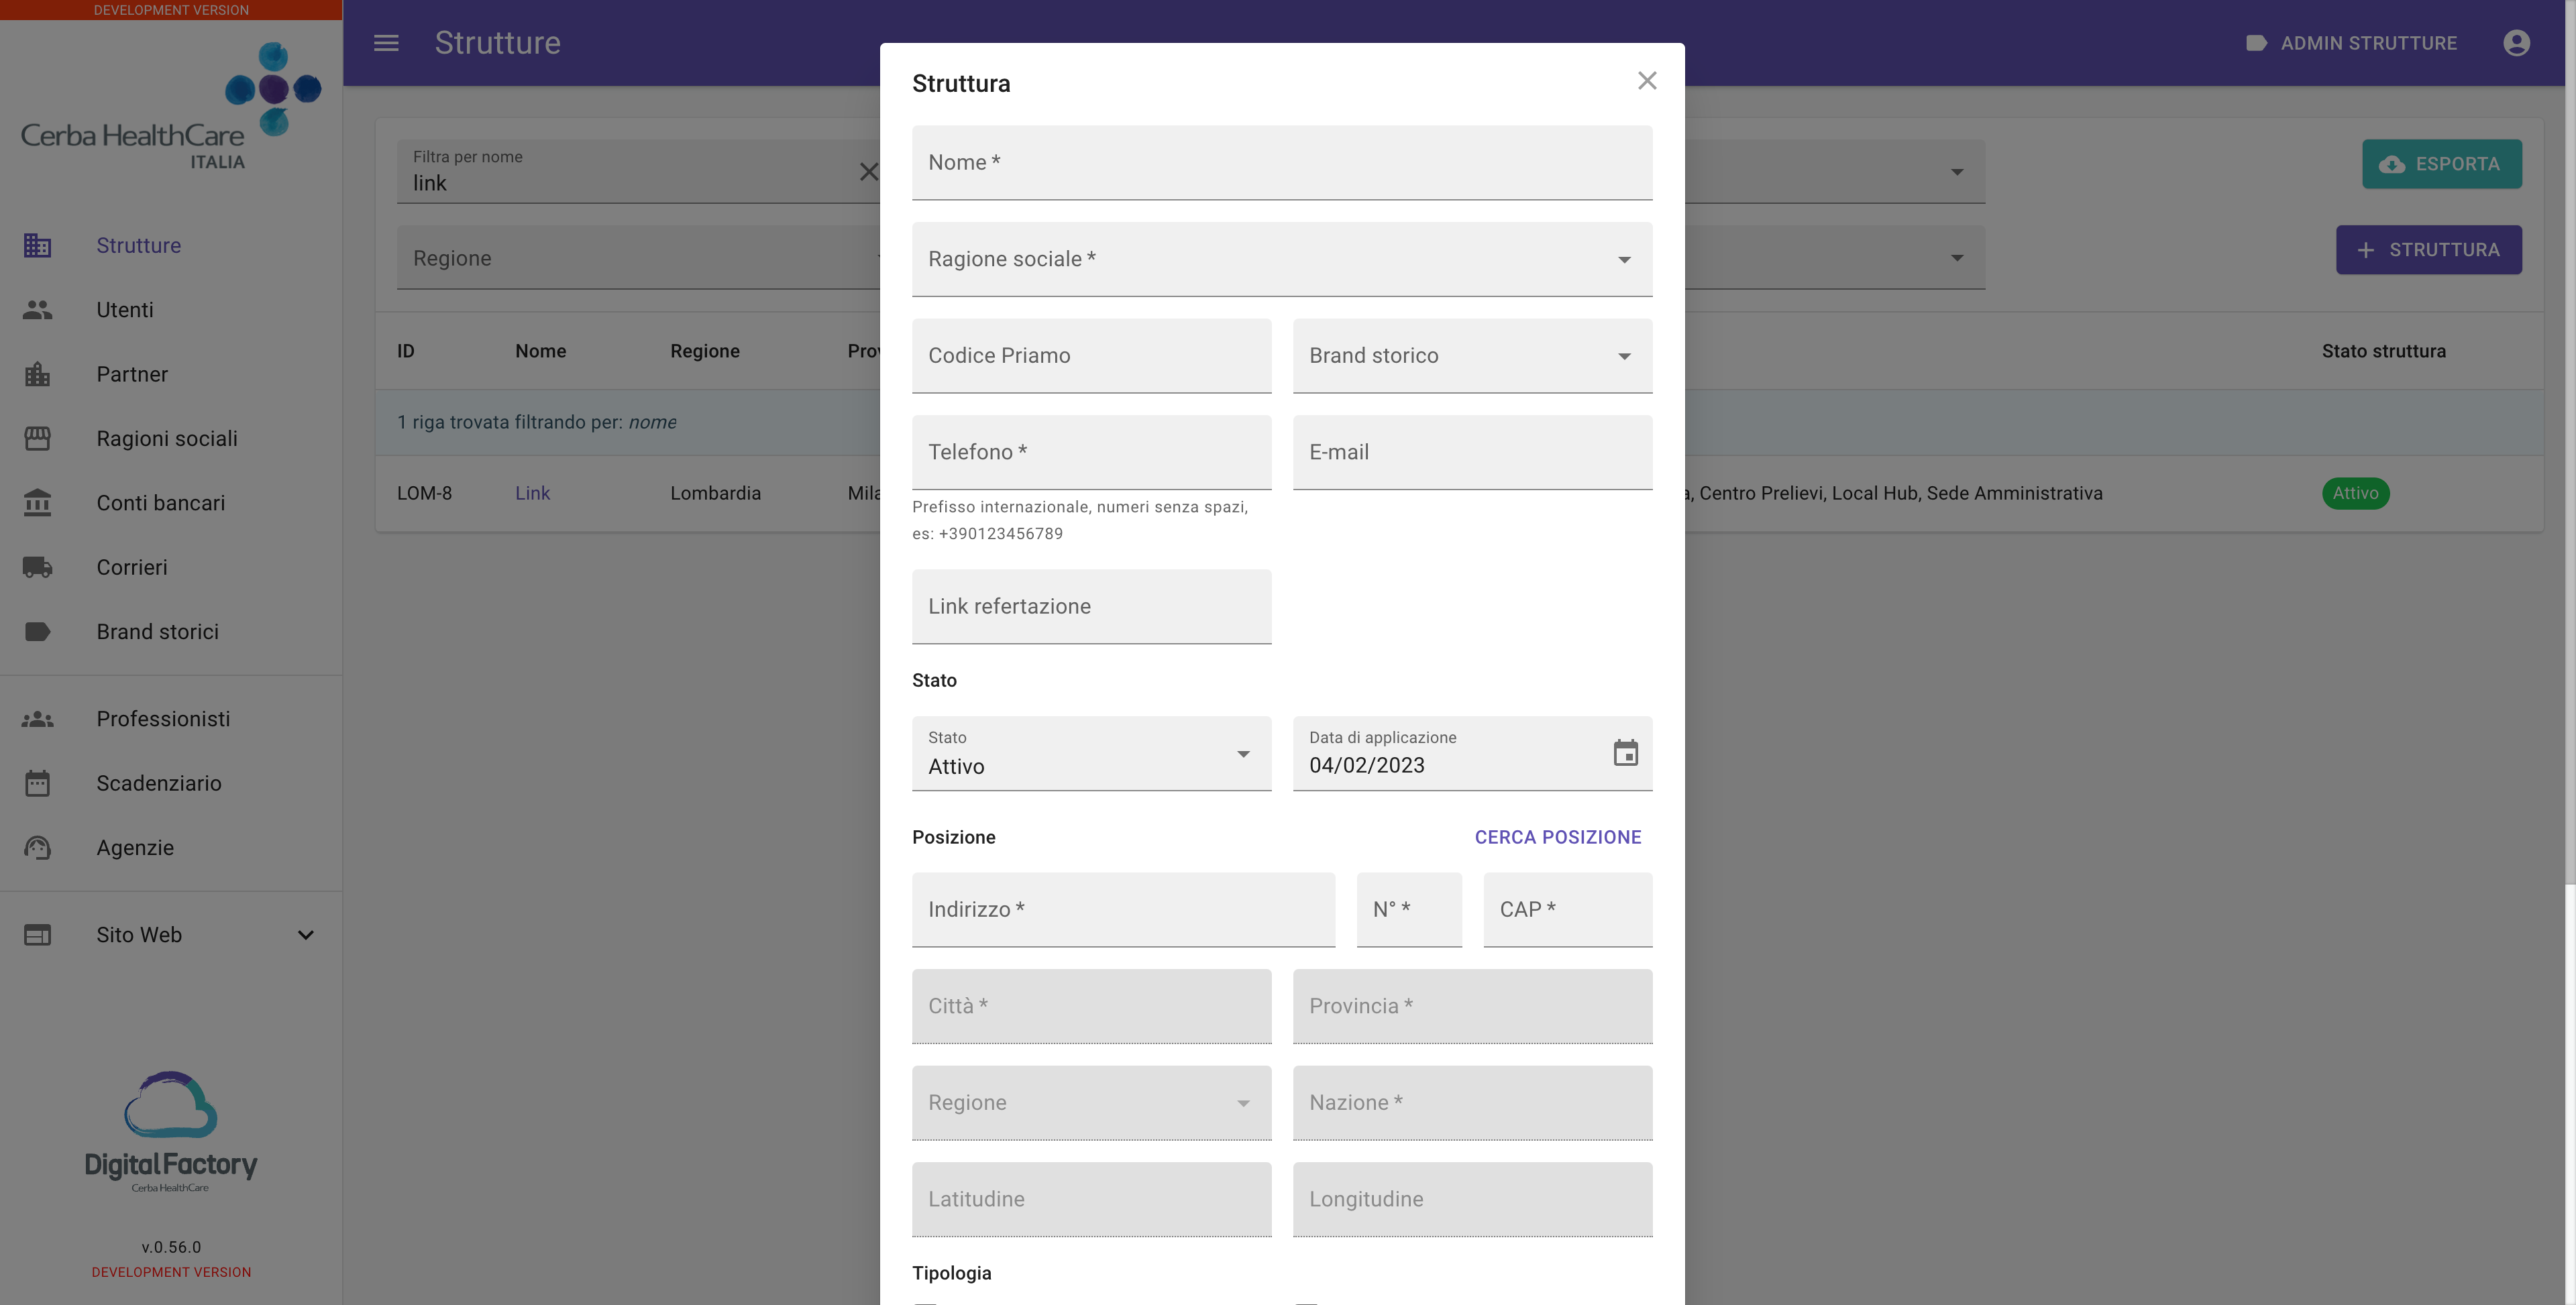
\includegraphics[width= 0.5\textwidth]{images/capitolo5/f1_f2_f3_websiteVisibility_email_links/ModalFacility_create_pt1.png} 
%     \caption{Modale aggiunta nuova struttura (pt1)} 
%     \label{fig:ModalFacility_create_pt1}
% \end{figure}

% \begin{figure}[H]
%     \centering
%     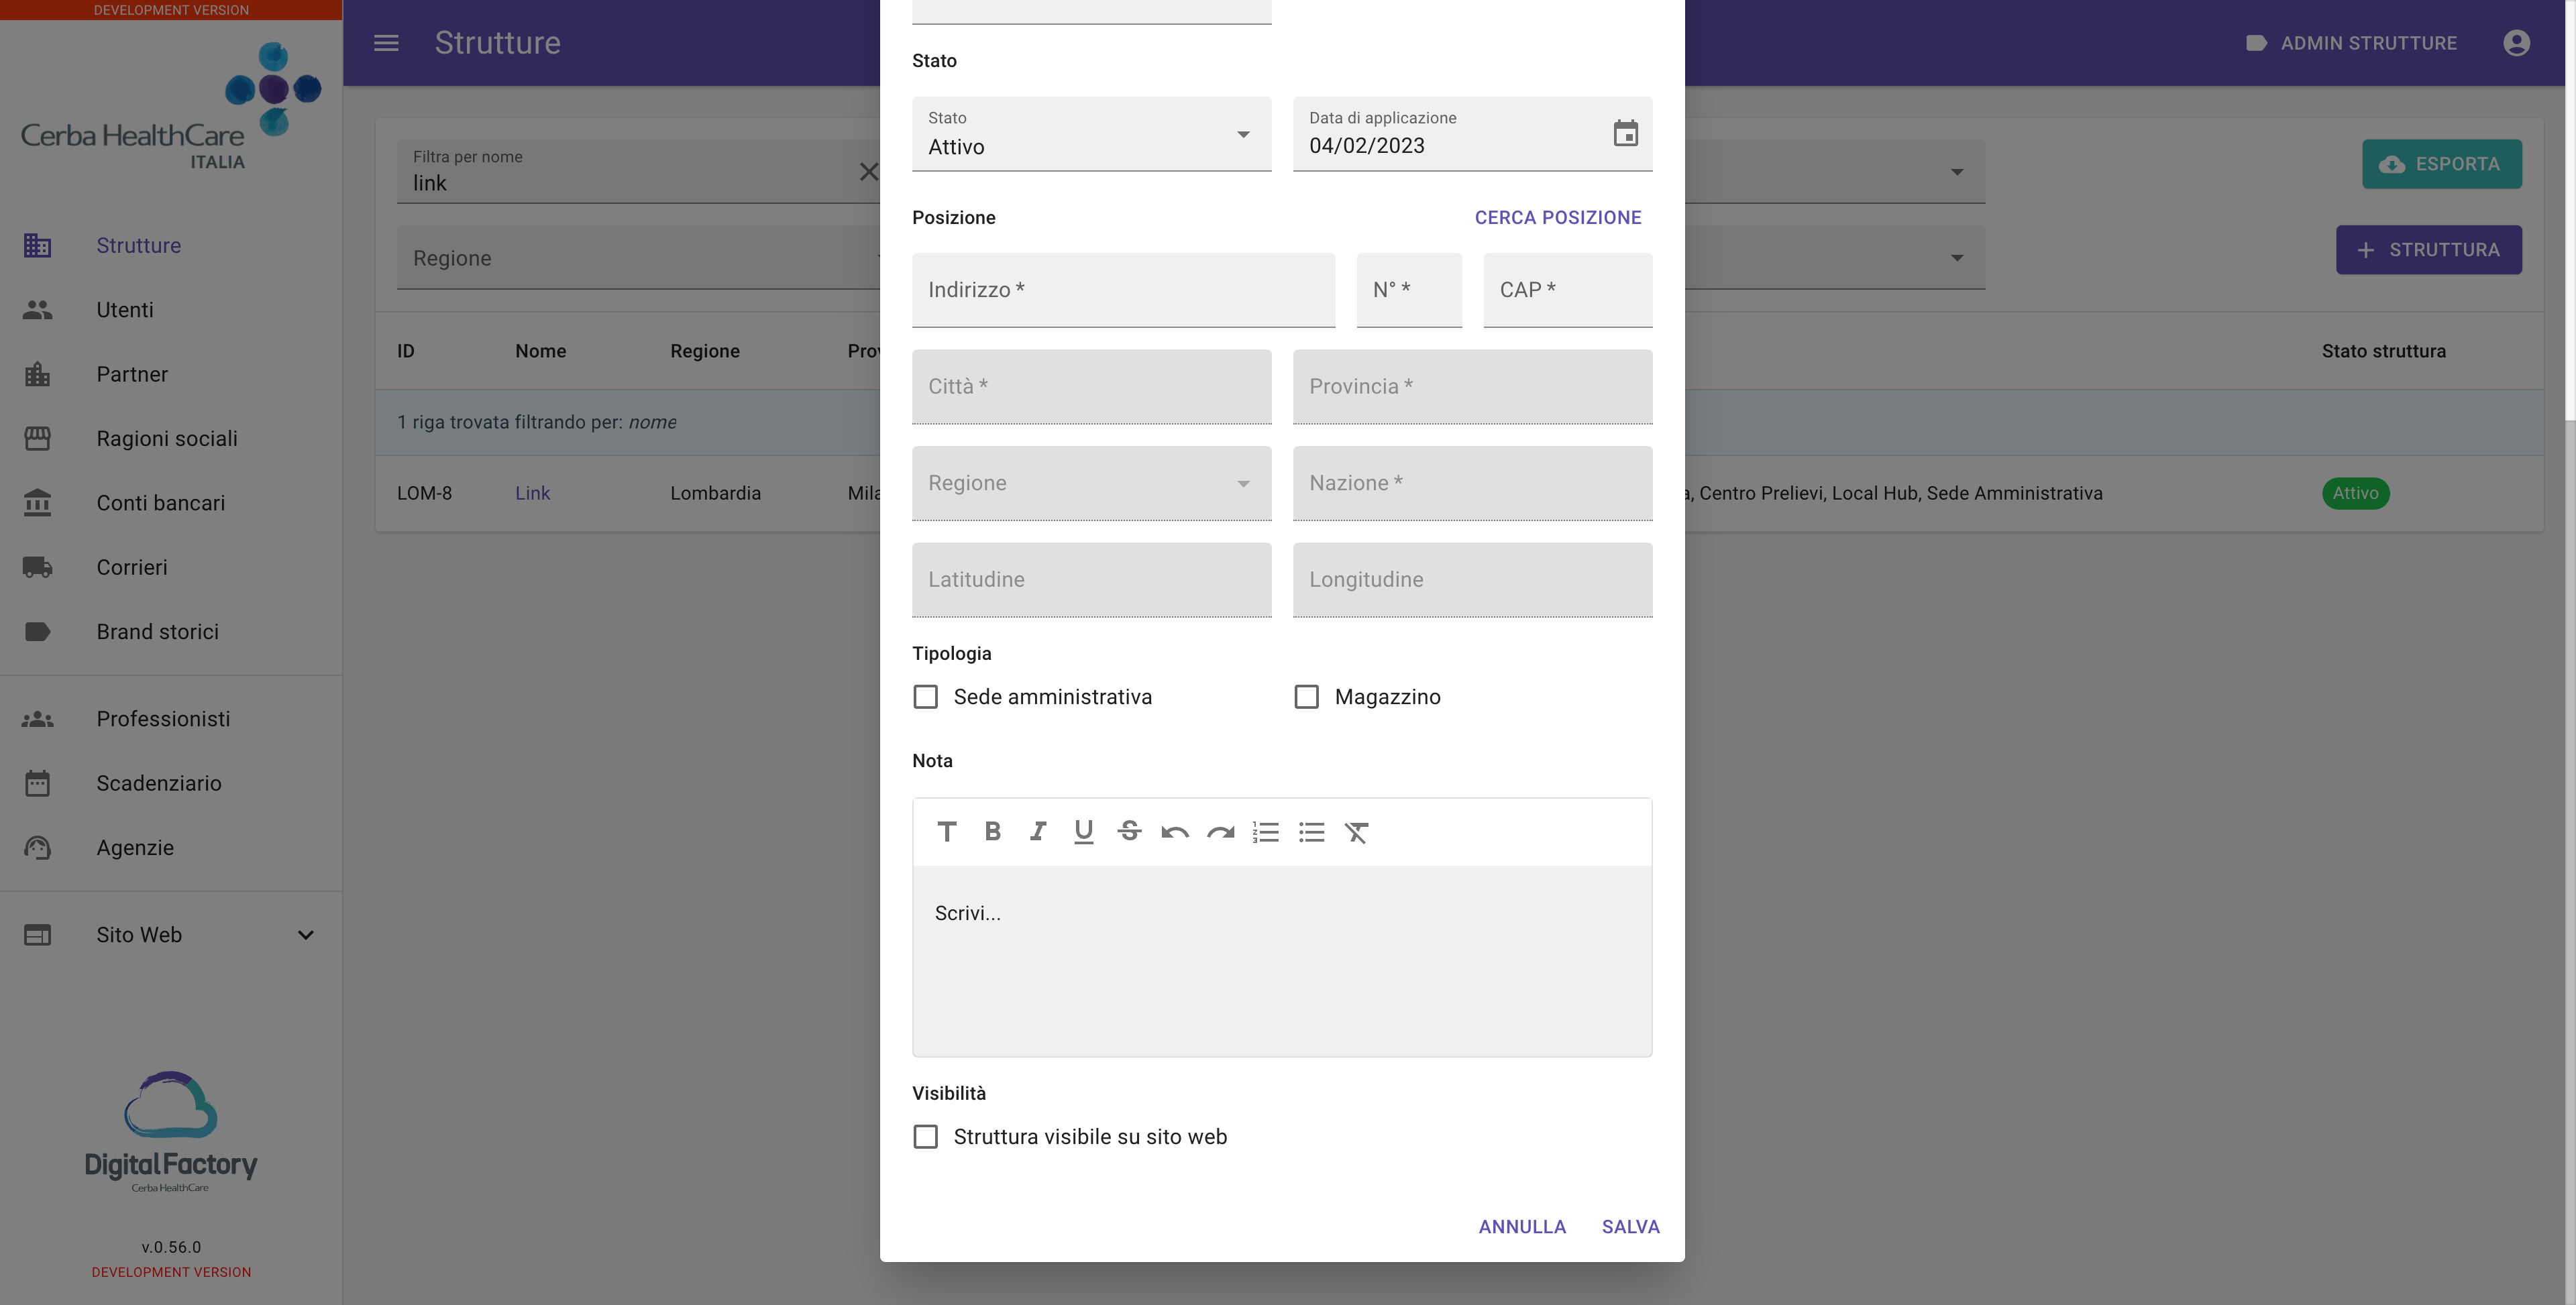
\includegraphics[width= 0.5\textwidth]{images/capitolo5/f1_f2_f3_websiteVisibility_email_links/ModalFacility_create_pt2.png} 
%     \caption{Modale aggiunta nuova struttura (pt2)} 
%     \label{fig:ModalFacility_create_pt2}
% \end{figure}

% \begin{figure}[H]
%     \centering
%     \subfloat[][\emph{Modale modifica parte 1}]
%         {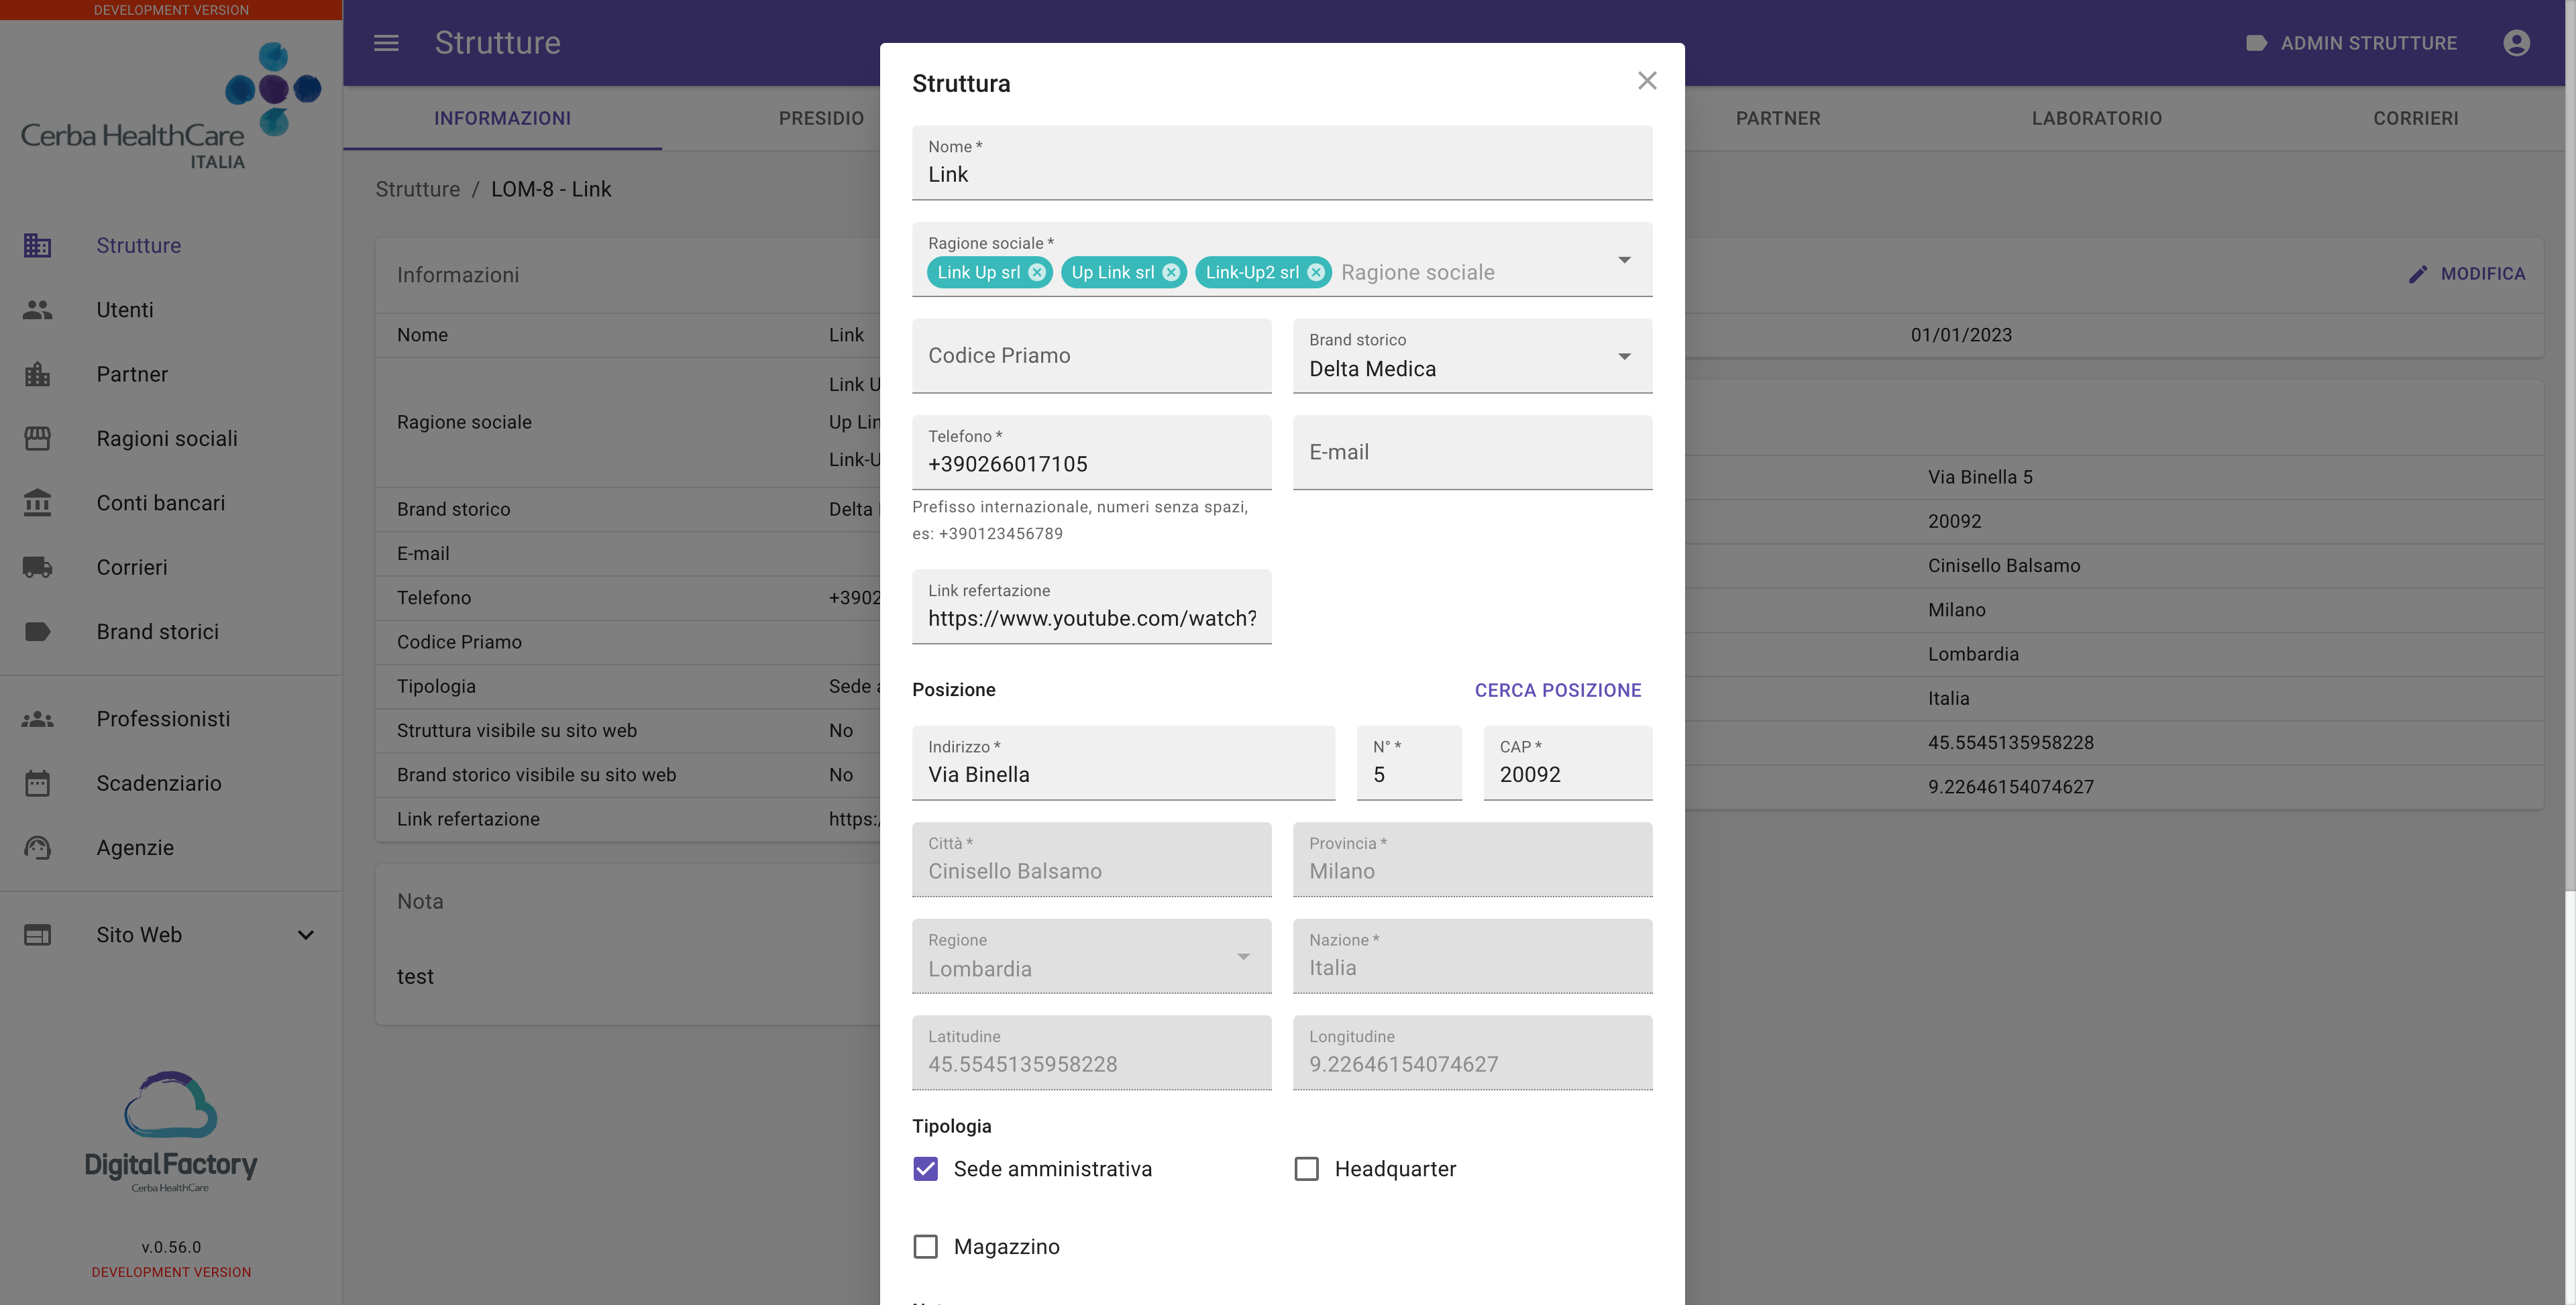
\includegraphics[width= 0.48\textwidth]{images/capitolo5/f1_f2_f3_websiteVisibility_email_links/ModalFacility_edit_pt1.png}} \quad
%     \subfloat[][\emph{Modale modifica parte 2}]
%         {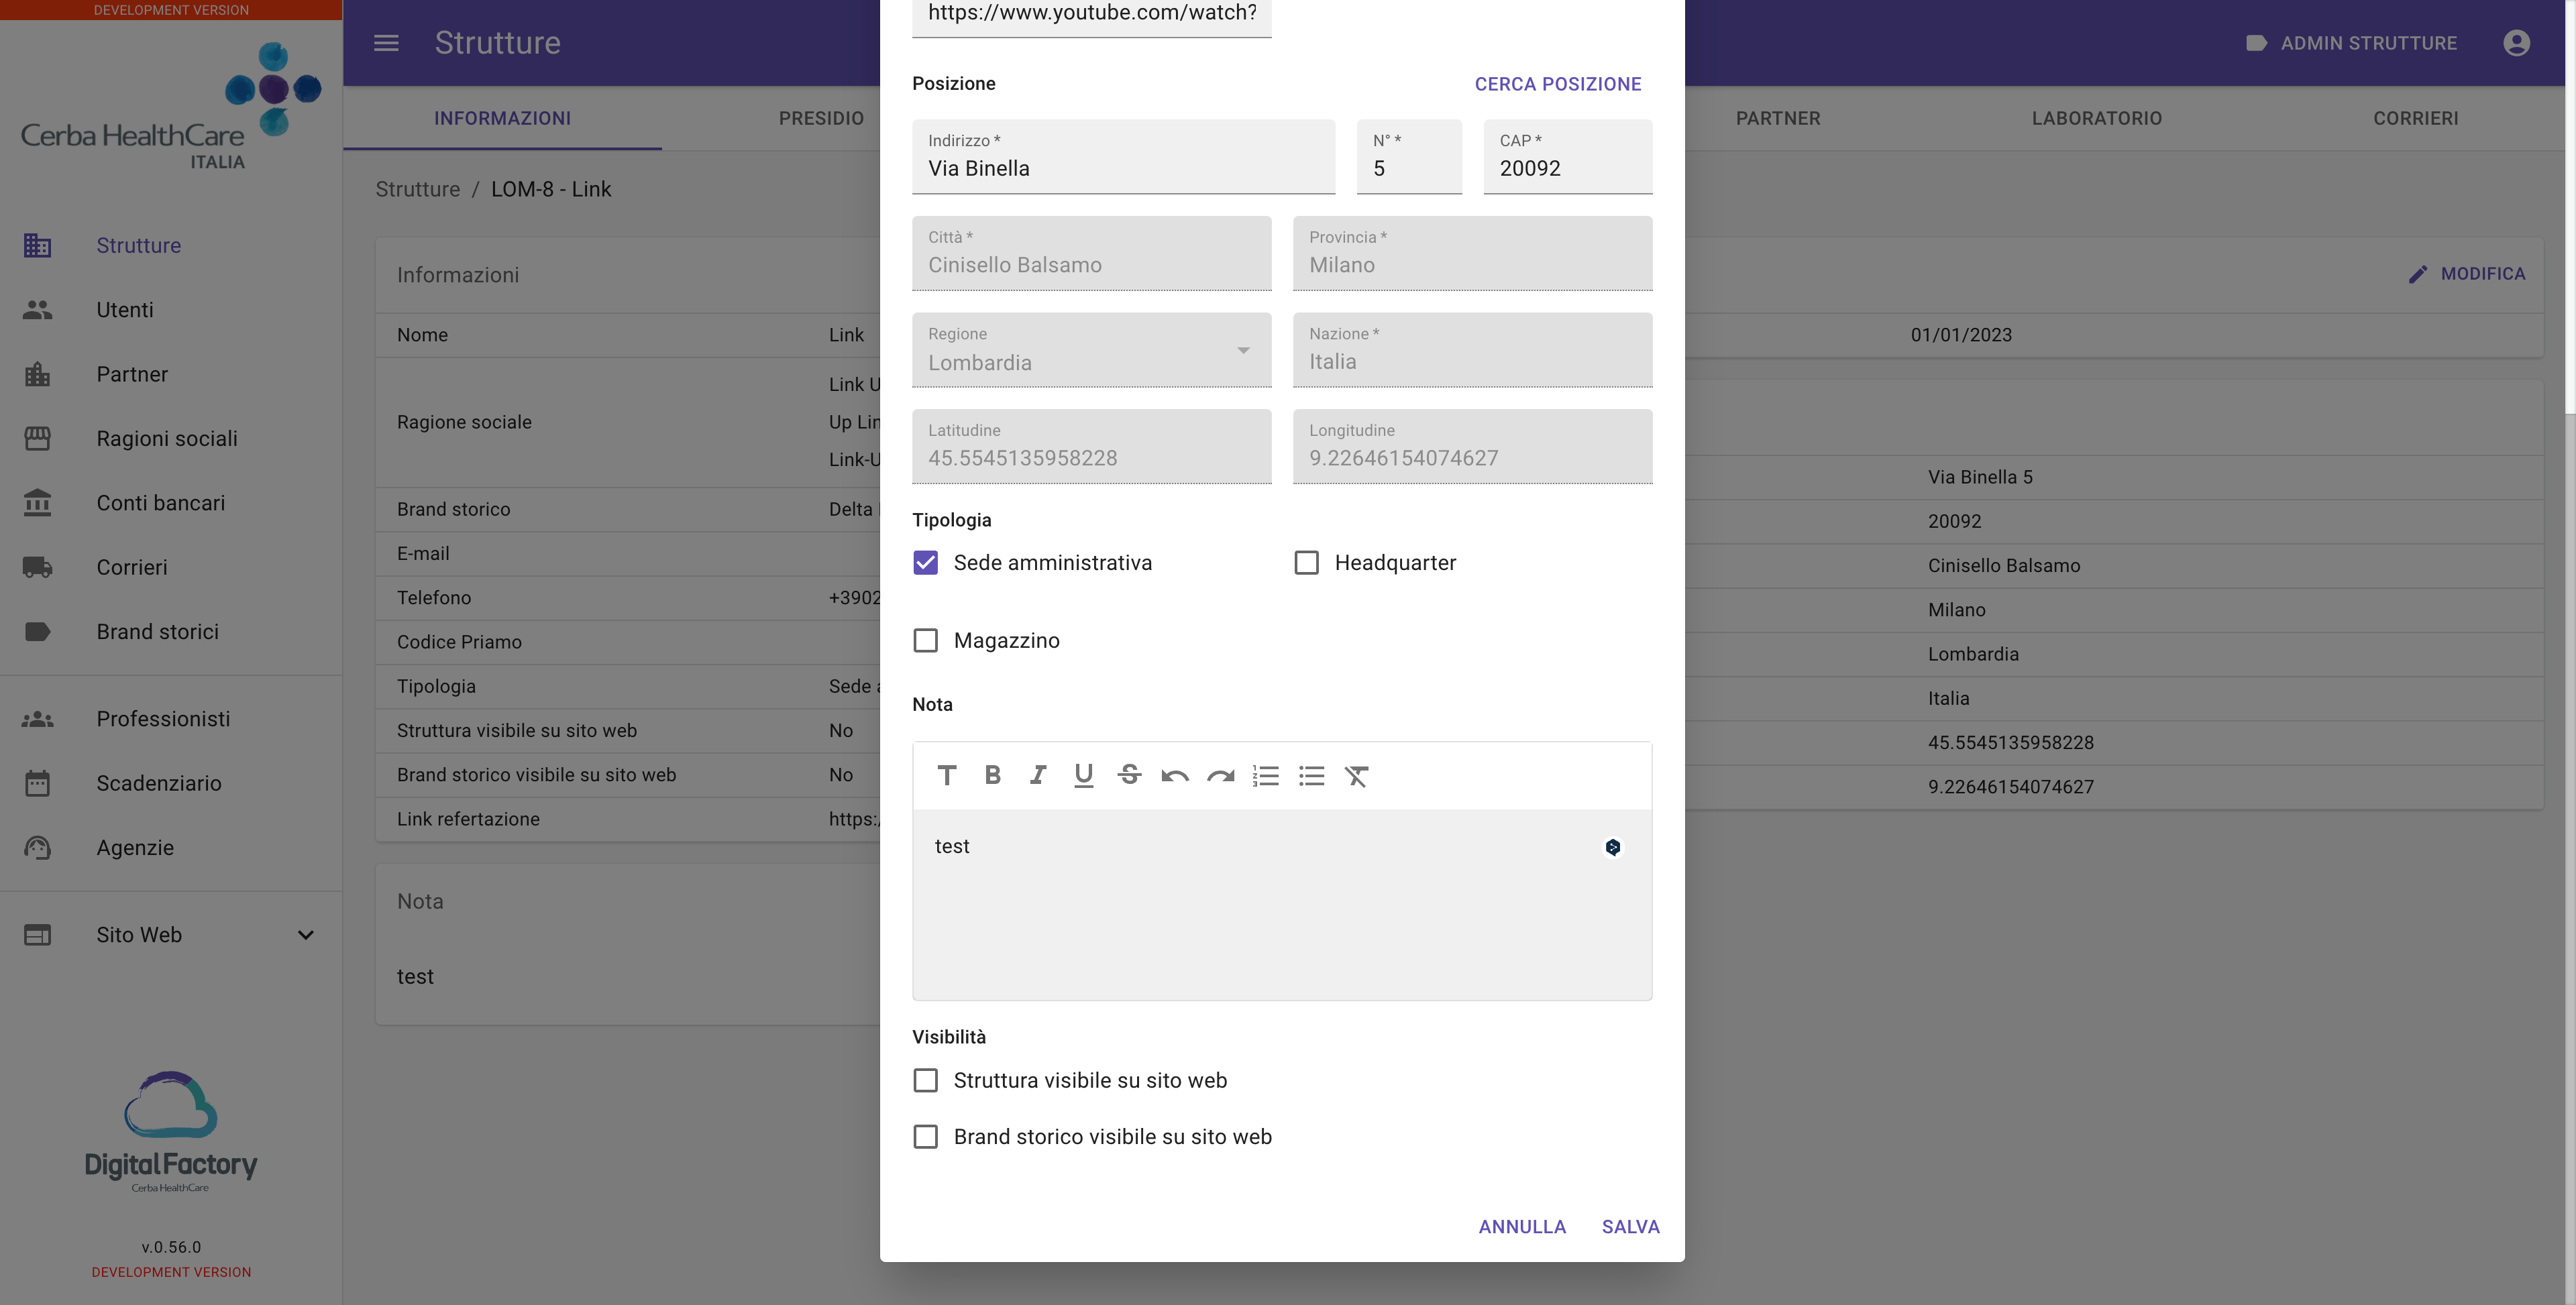
\includegraphics[width= 0.48\textwidth]{images/capitolo5/f1_f2_f3_websiteVisibility_email_links/ModalFacility_edit_pt2.png}} 
%     \caption{Modale modifica struttura esistente}
%     % \label{fig:Modale modifica struttura esistente}    
% \end{figure}

% \begin{figure}[H]
%     \centering
%     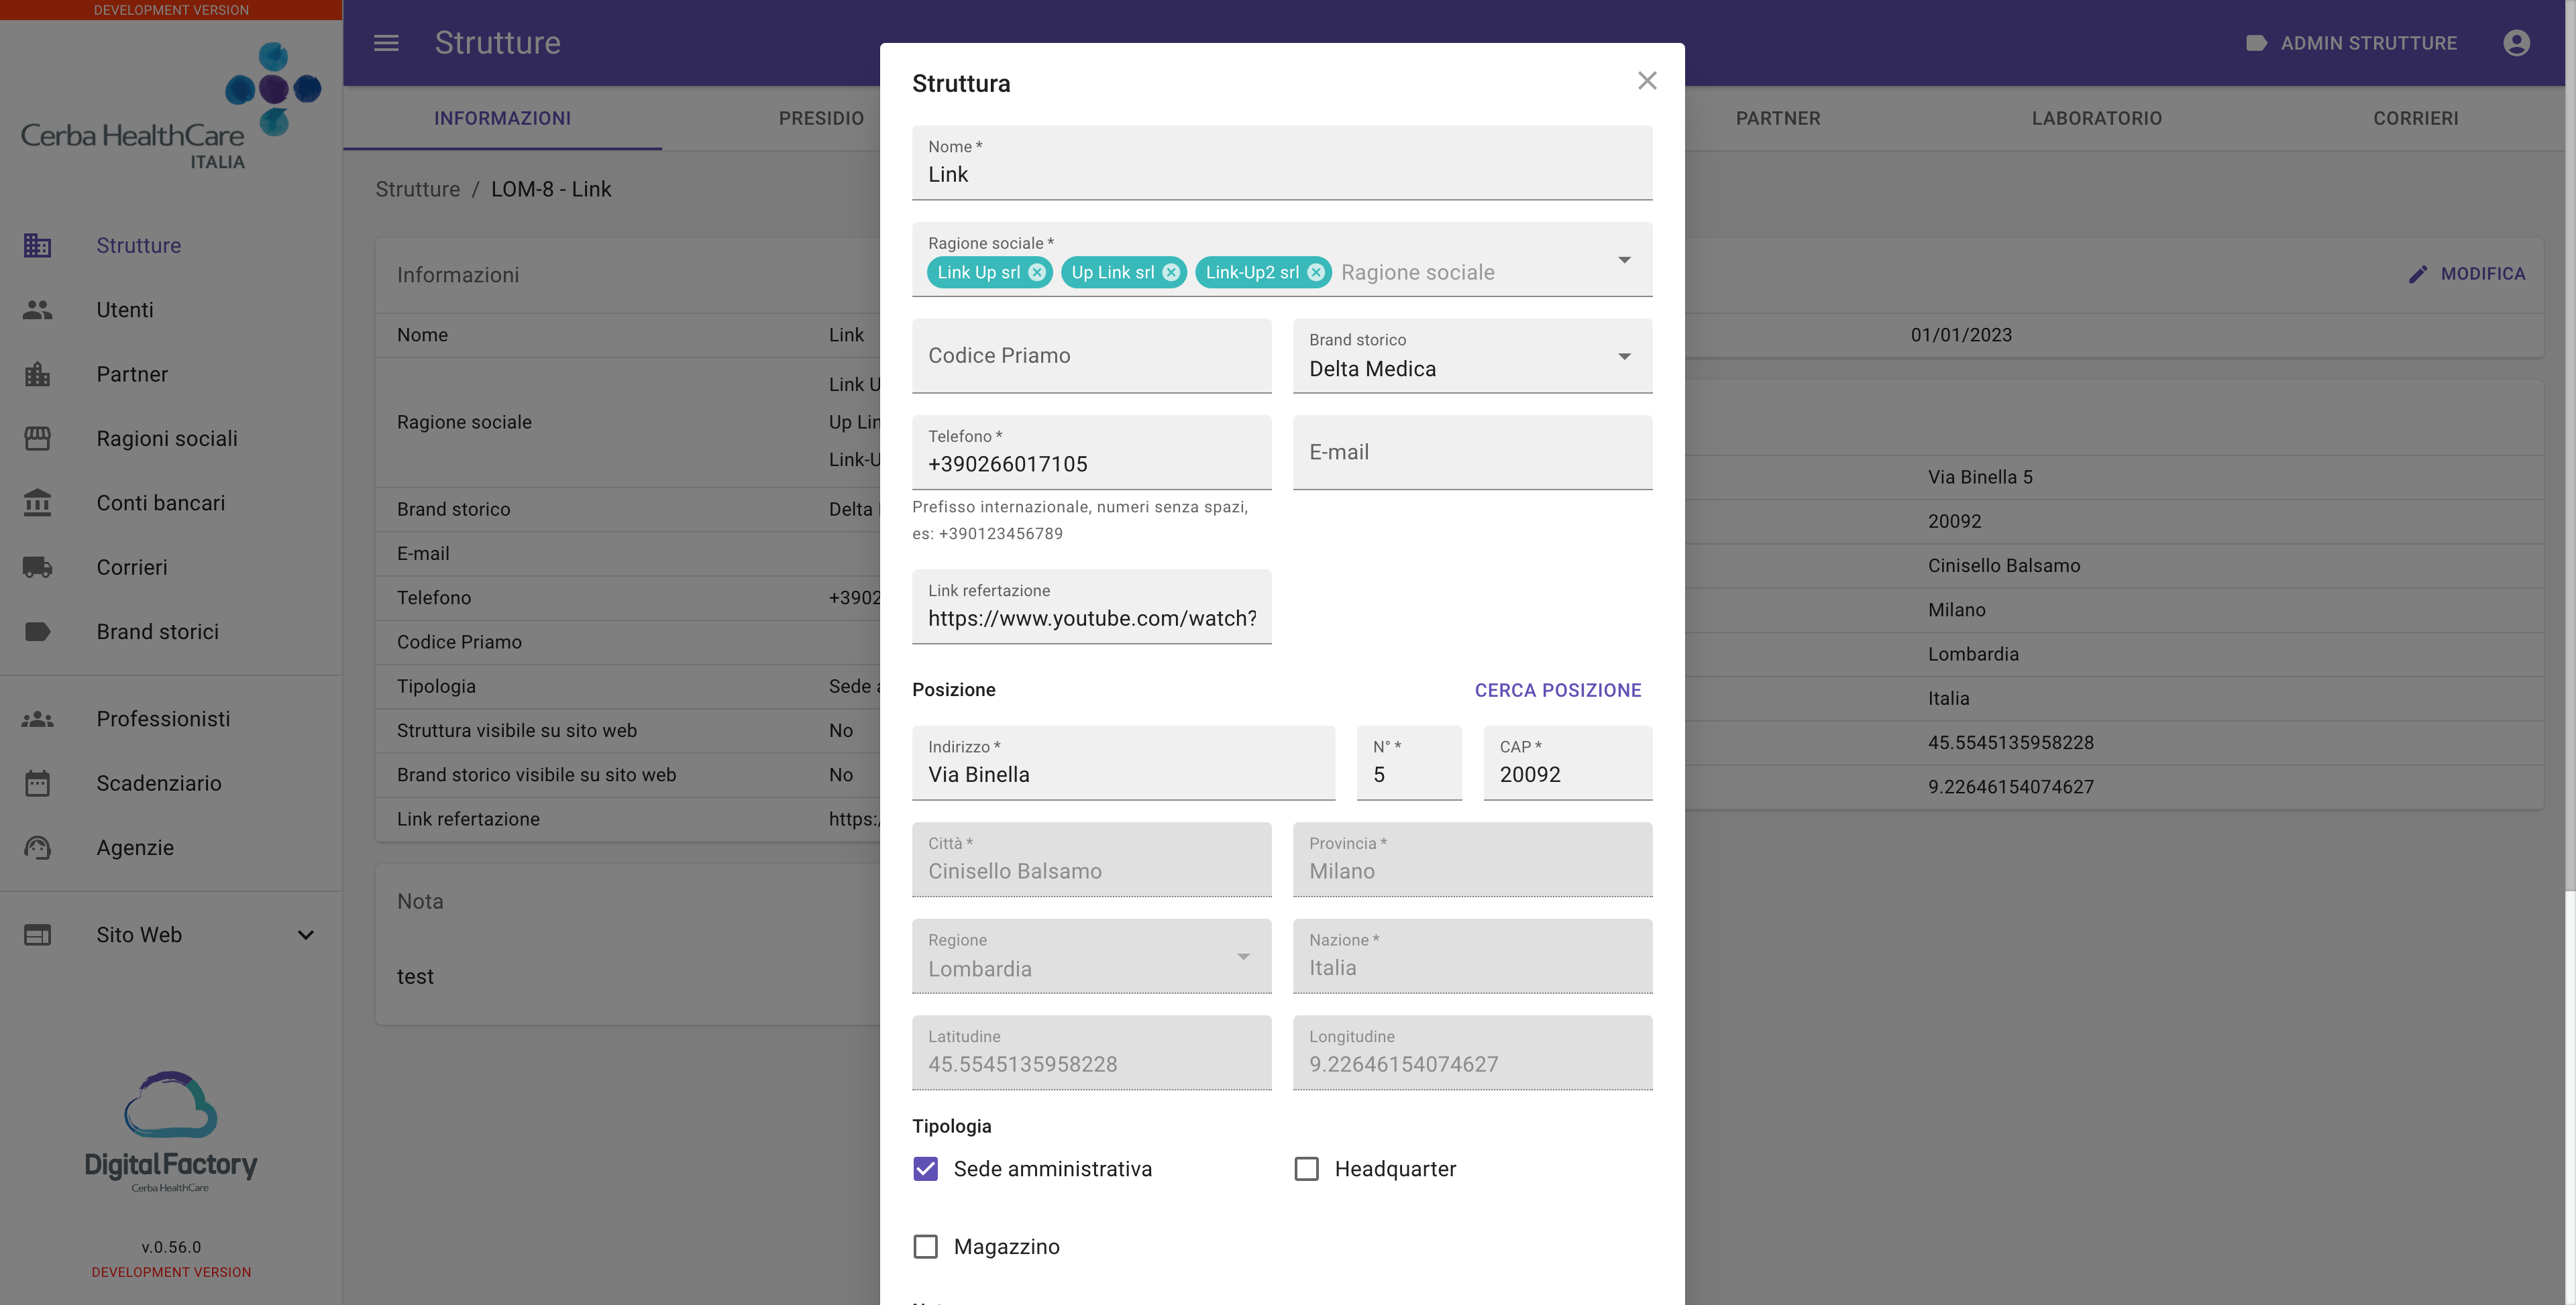
\includegraphics[width= 0.5\textwidth]{images/capitolo5/f1_f2_f3_websiteVisibility_email_links/ModalFacility_edit_pt1.png} 
%     \caption{Modale modifica struttura esistente (pt1)} 
%     \label{fig:ModalFacility_edit_pt1}
% \end{figure}

% \begin{figure}[H]
%     \centering
%     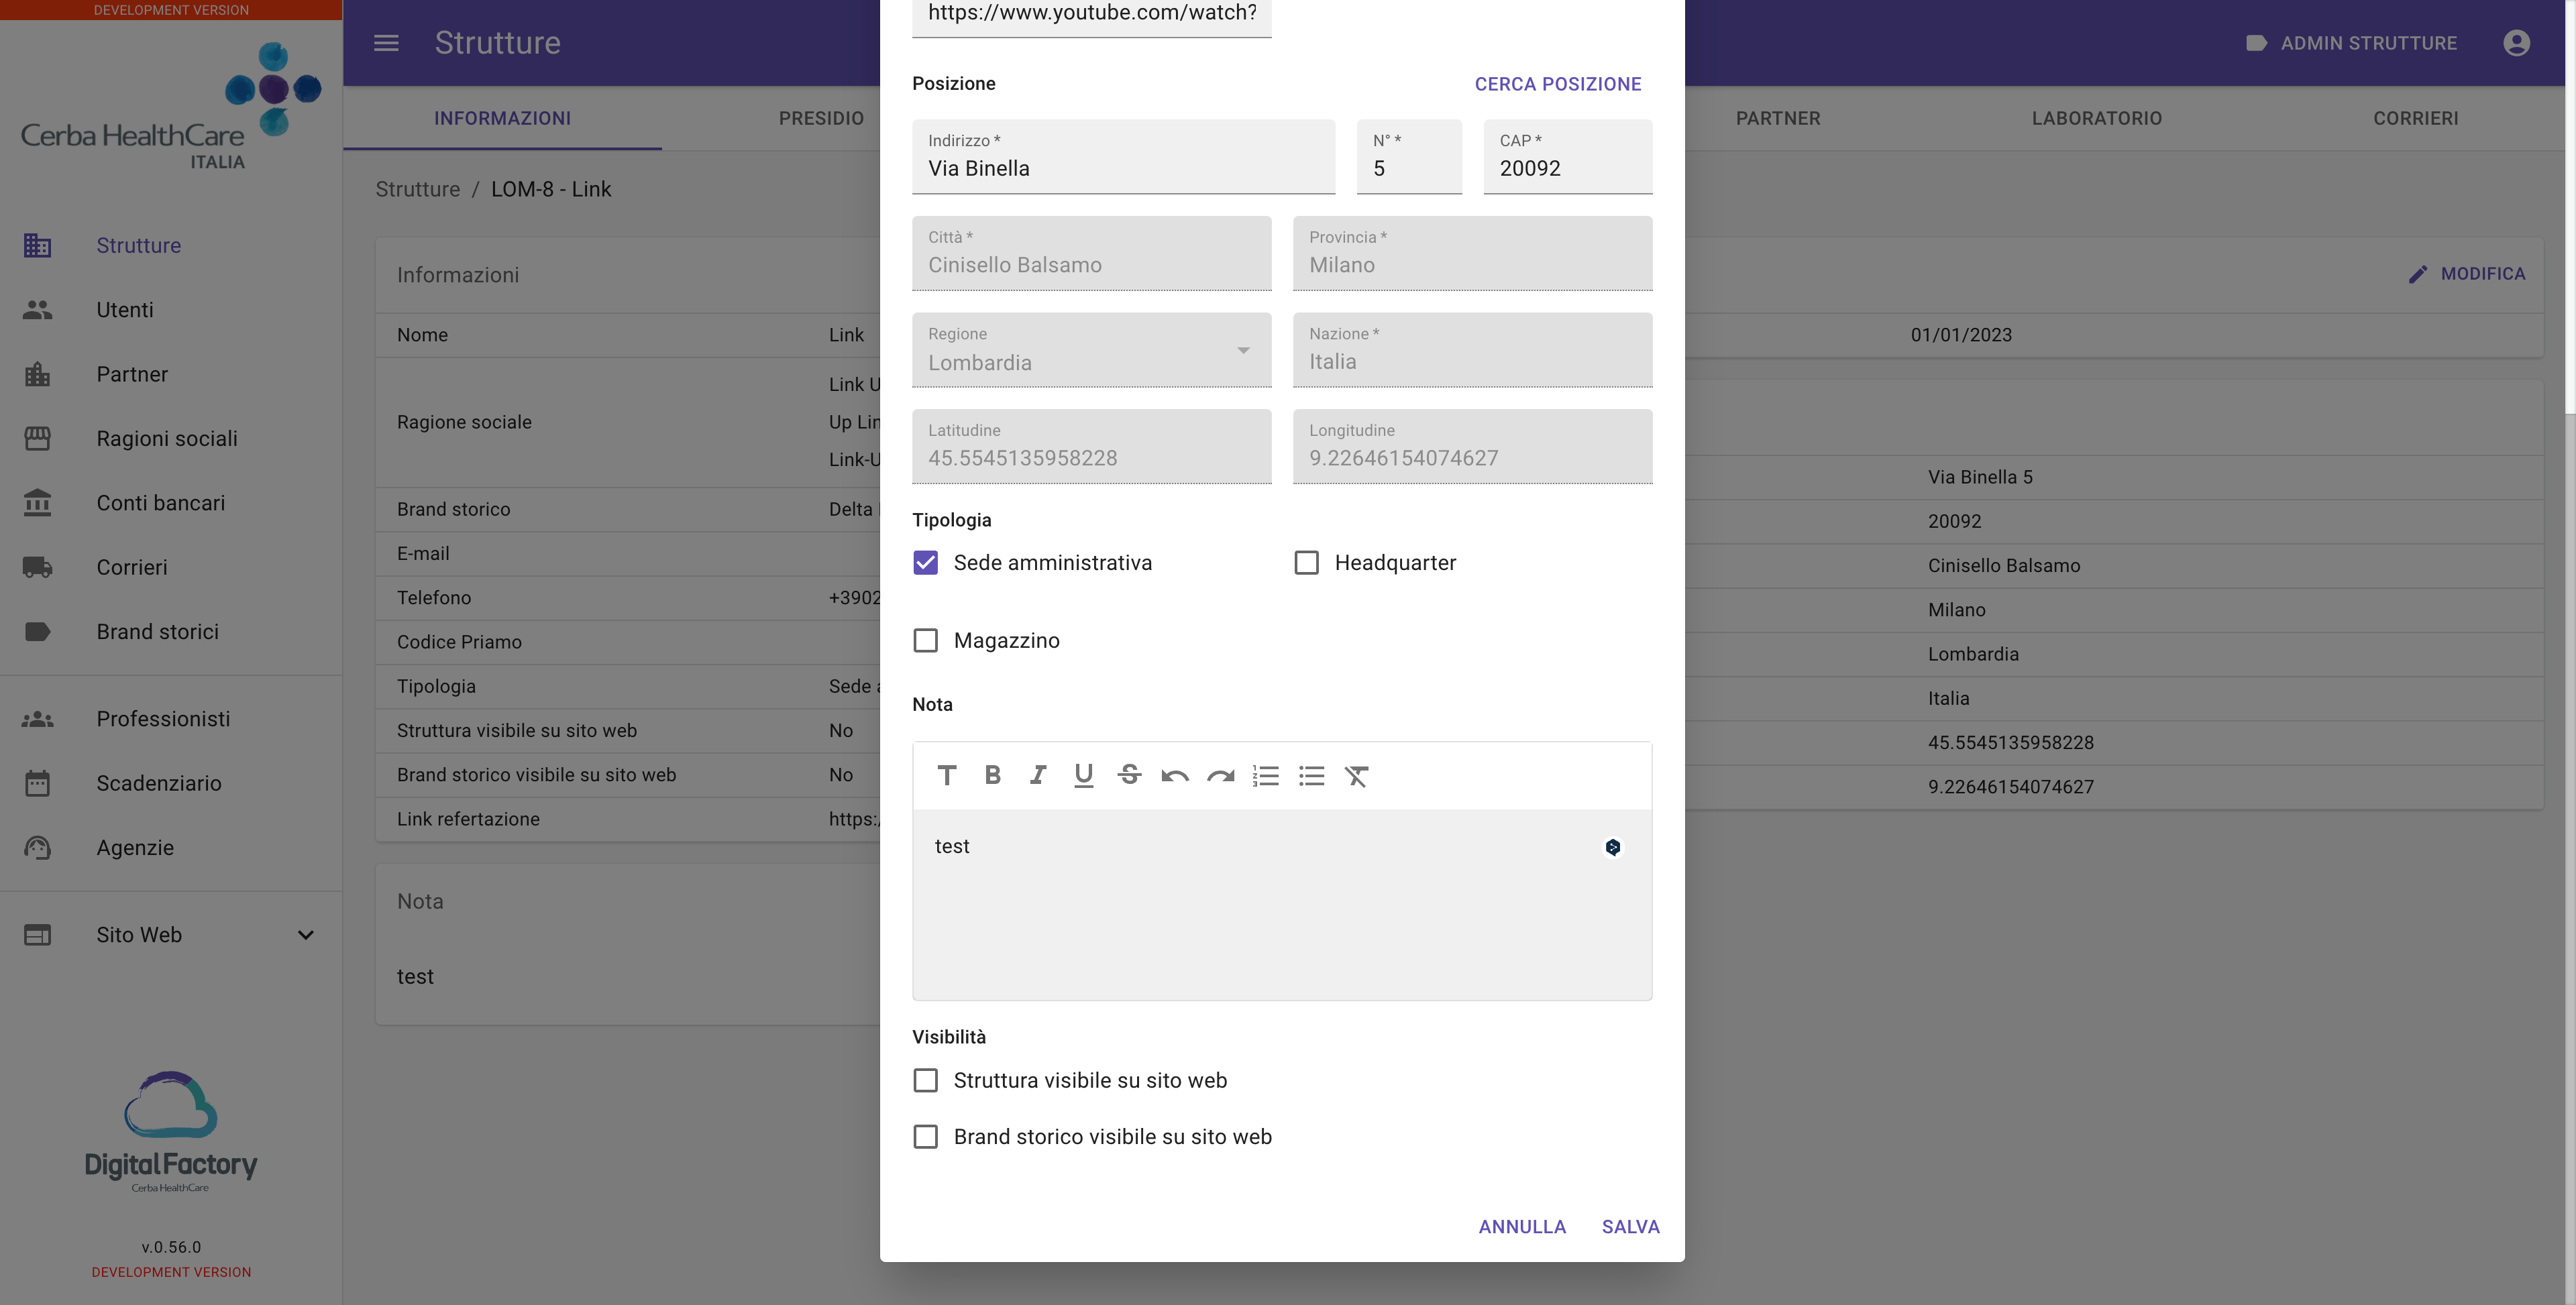
\includegraphics[width= 0.5\textwidth]{images/capitolo5/f1_f2_f3_websiteVisibility_email_links/ModalFacility_edit_pt2.png} 
%     \caption{Modale modifica struttura esistente (pt2)} 
%     \label{fig:ModalFacility_edit_pt2}
% \end{figure}

\begin{figure}[H]
    \centering
    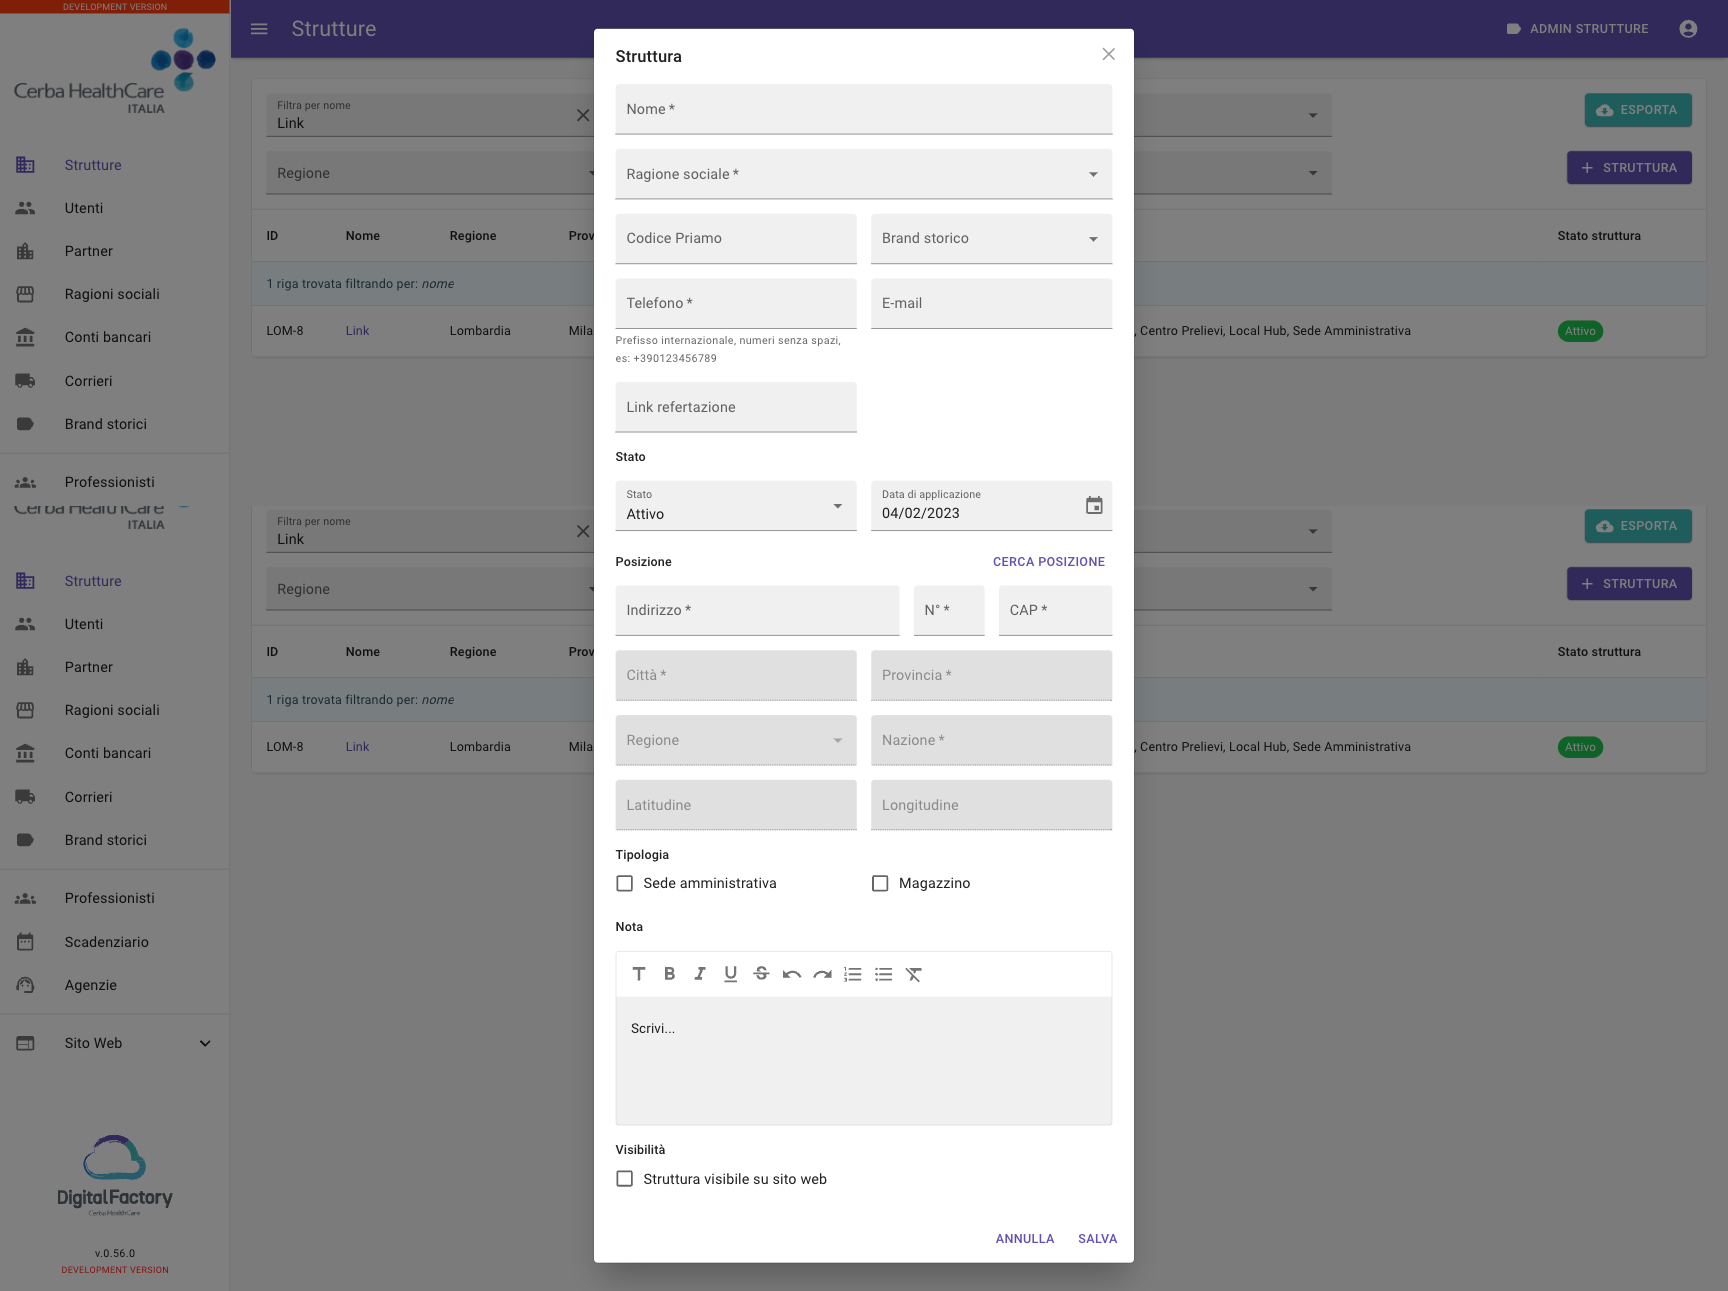
\includegraphics[width= 0.7\textwidth]{images/capitolo5/f1_f2_f3_websiteVisibility_email_links/ModalFacility_create.png} 
    \caption{Modale aggiunta nuova struttura} 
    \label{fig:ModalFacility_create}
\end{figure}

\begin{figure}[H]
    \centering
    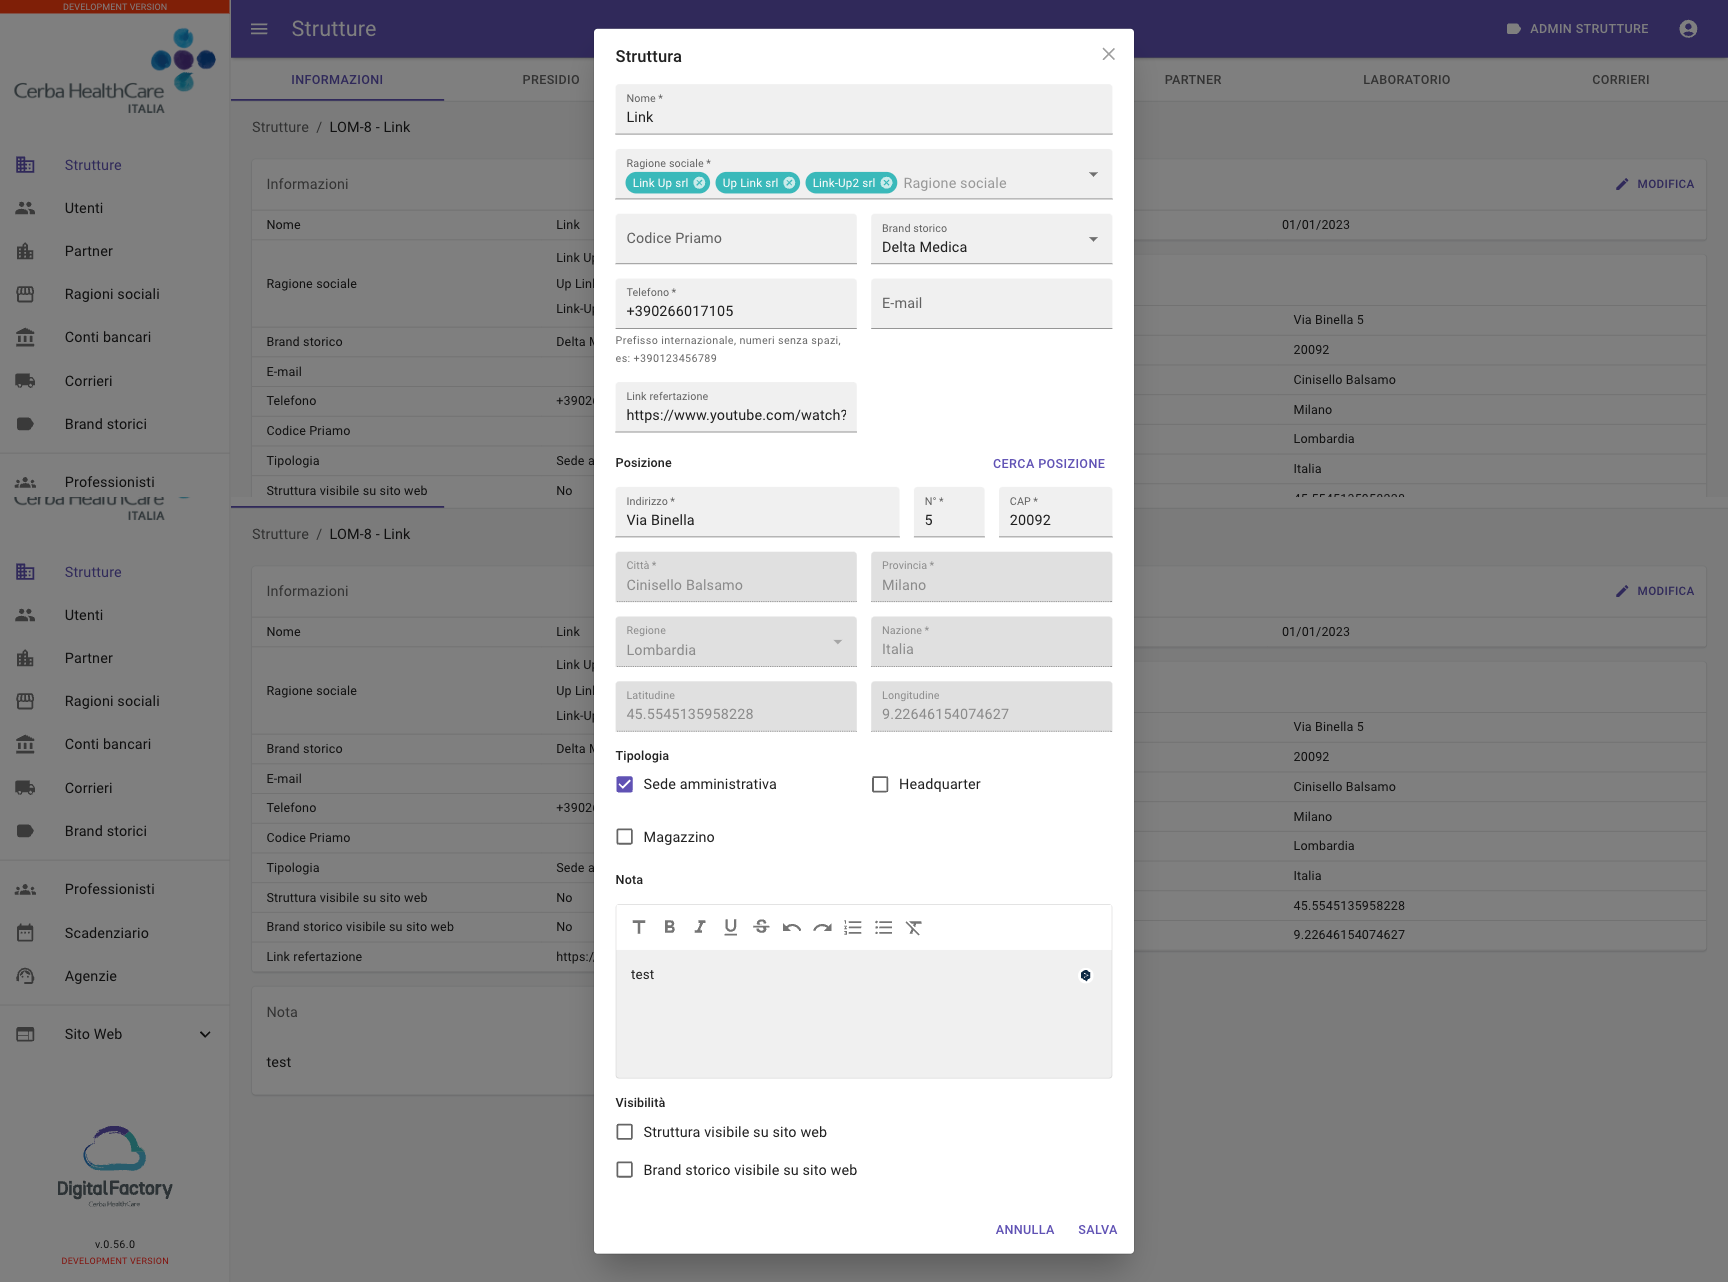
\includegraphics[width= 0.7\textwidth]{images/capitolo5/f1_f2_f3_websiteVisibility_email_links/ModalFacility_edit.png} 
    \caption{Modale modifica struttura esistente} 
    \label{fig:ModalFacility_edit}
\end{figure}

\newpage
\begin{figure}[H]
    \centering
    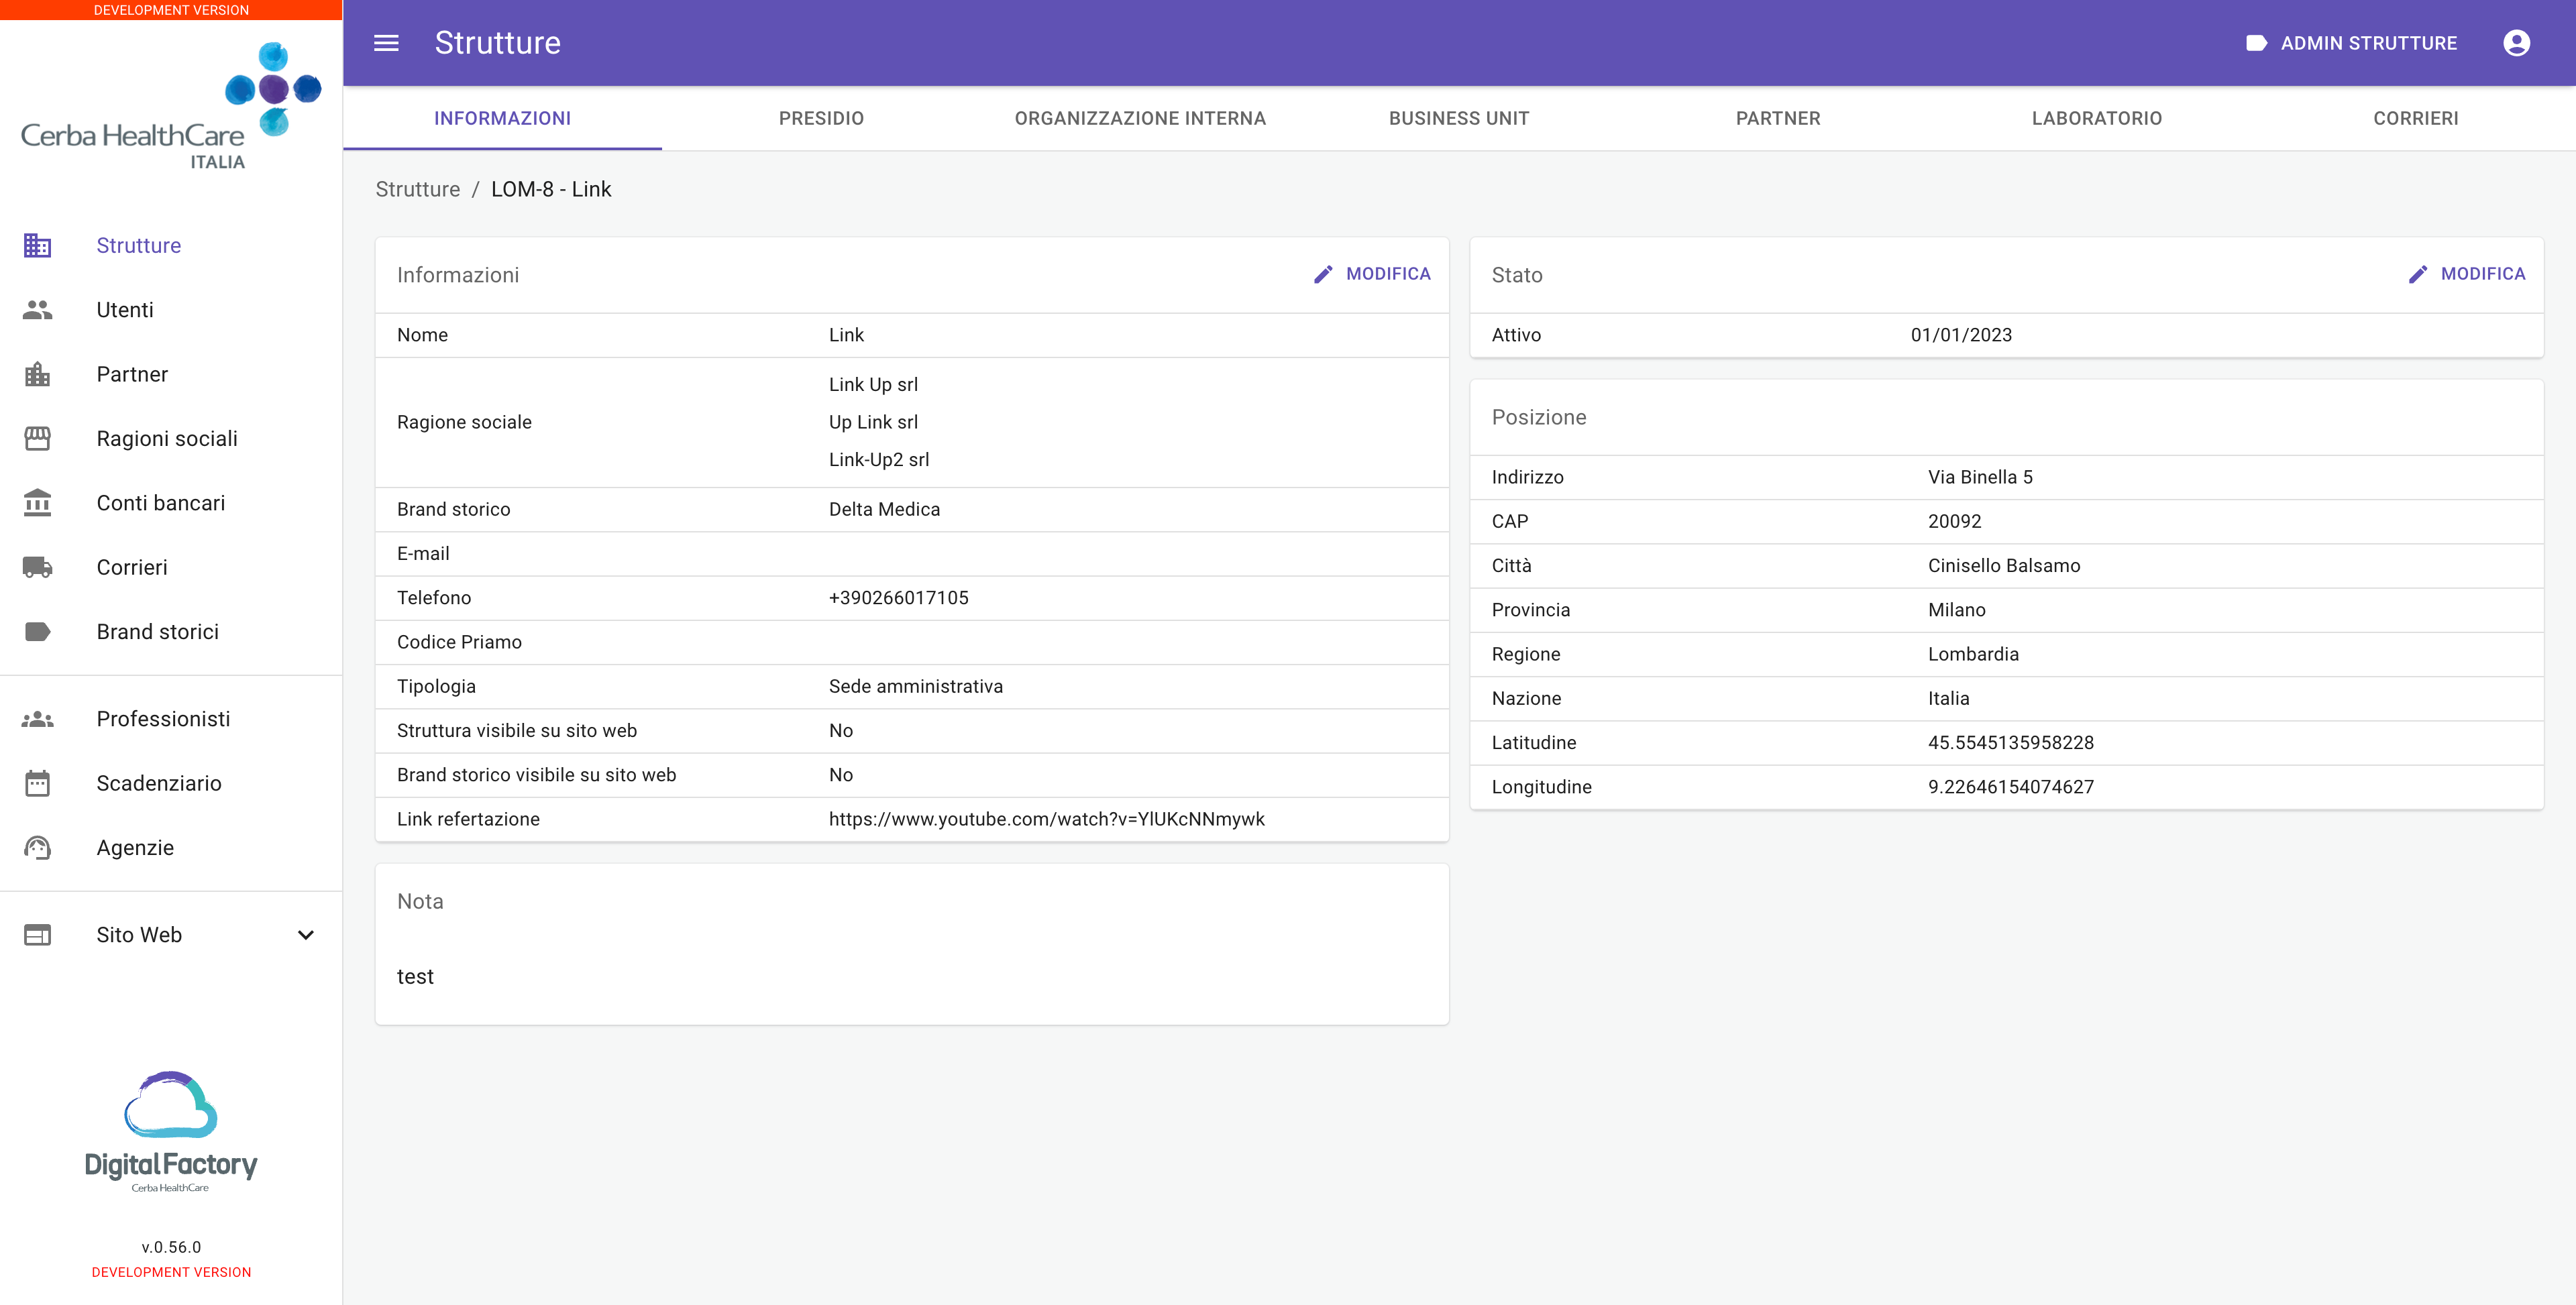
\includegraphics[width= 0.75\textwidth]{images/capitolo5/f1_f2_f3_websiteVisibility_email_links/TabInfo.png} 
    \caption{Tabella informazioni struttura} 
    \label{fig:TabInfo}
\end{figure}

\begin{figure}[H]
    \centering
    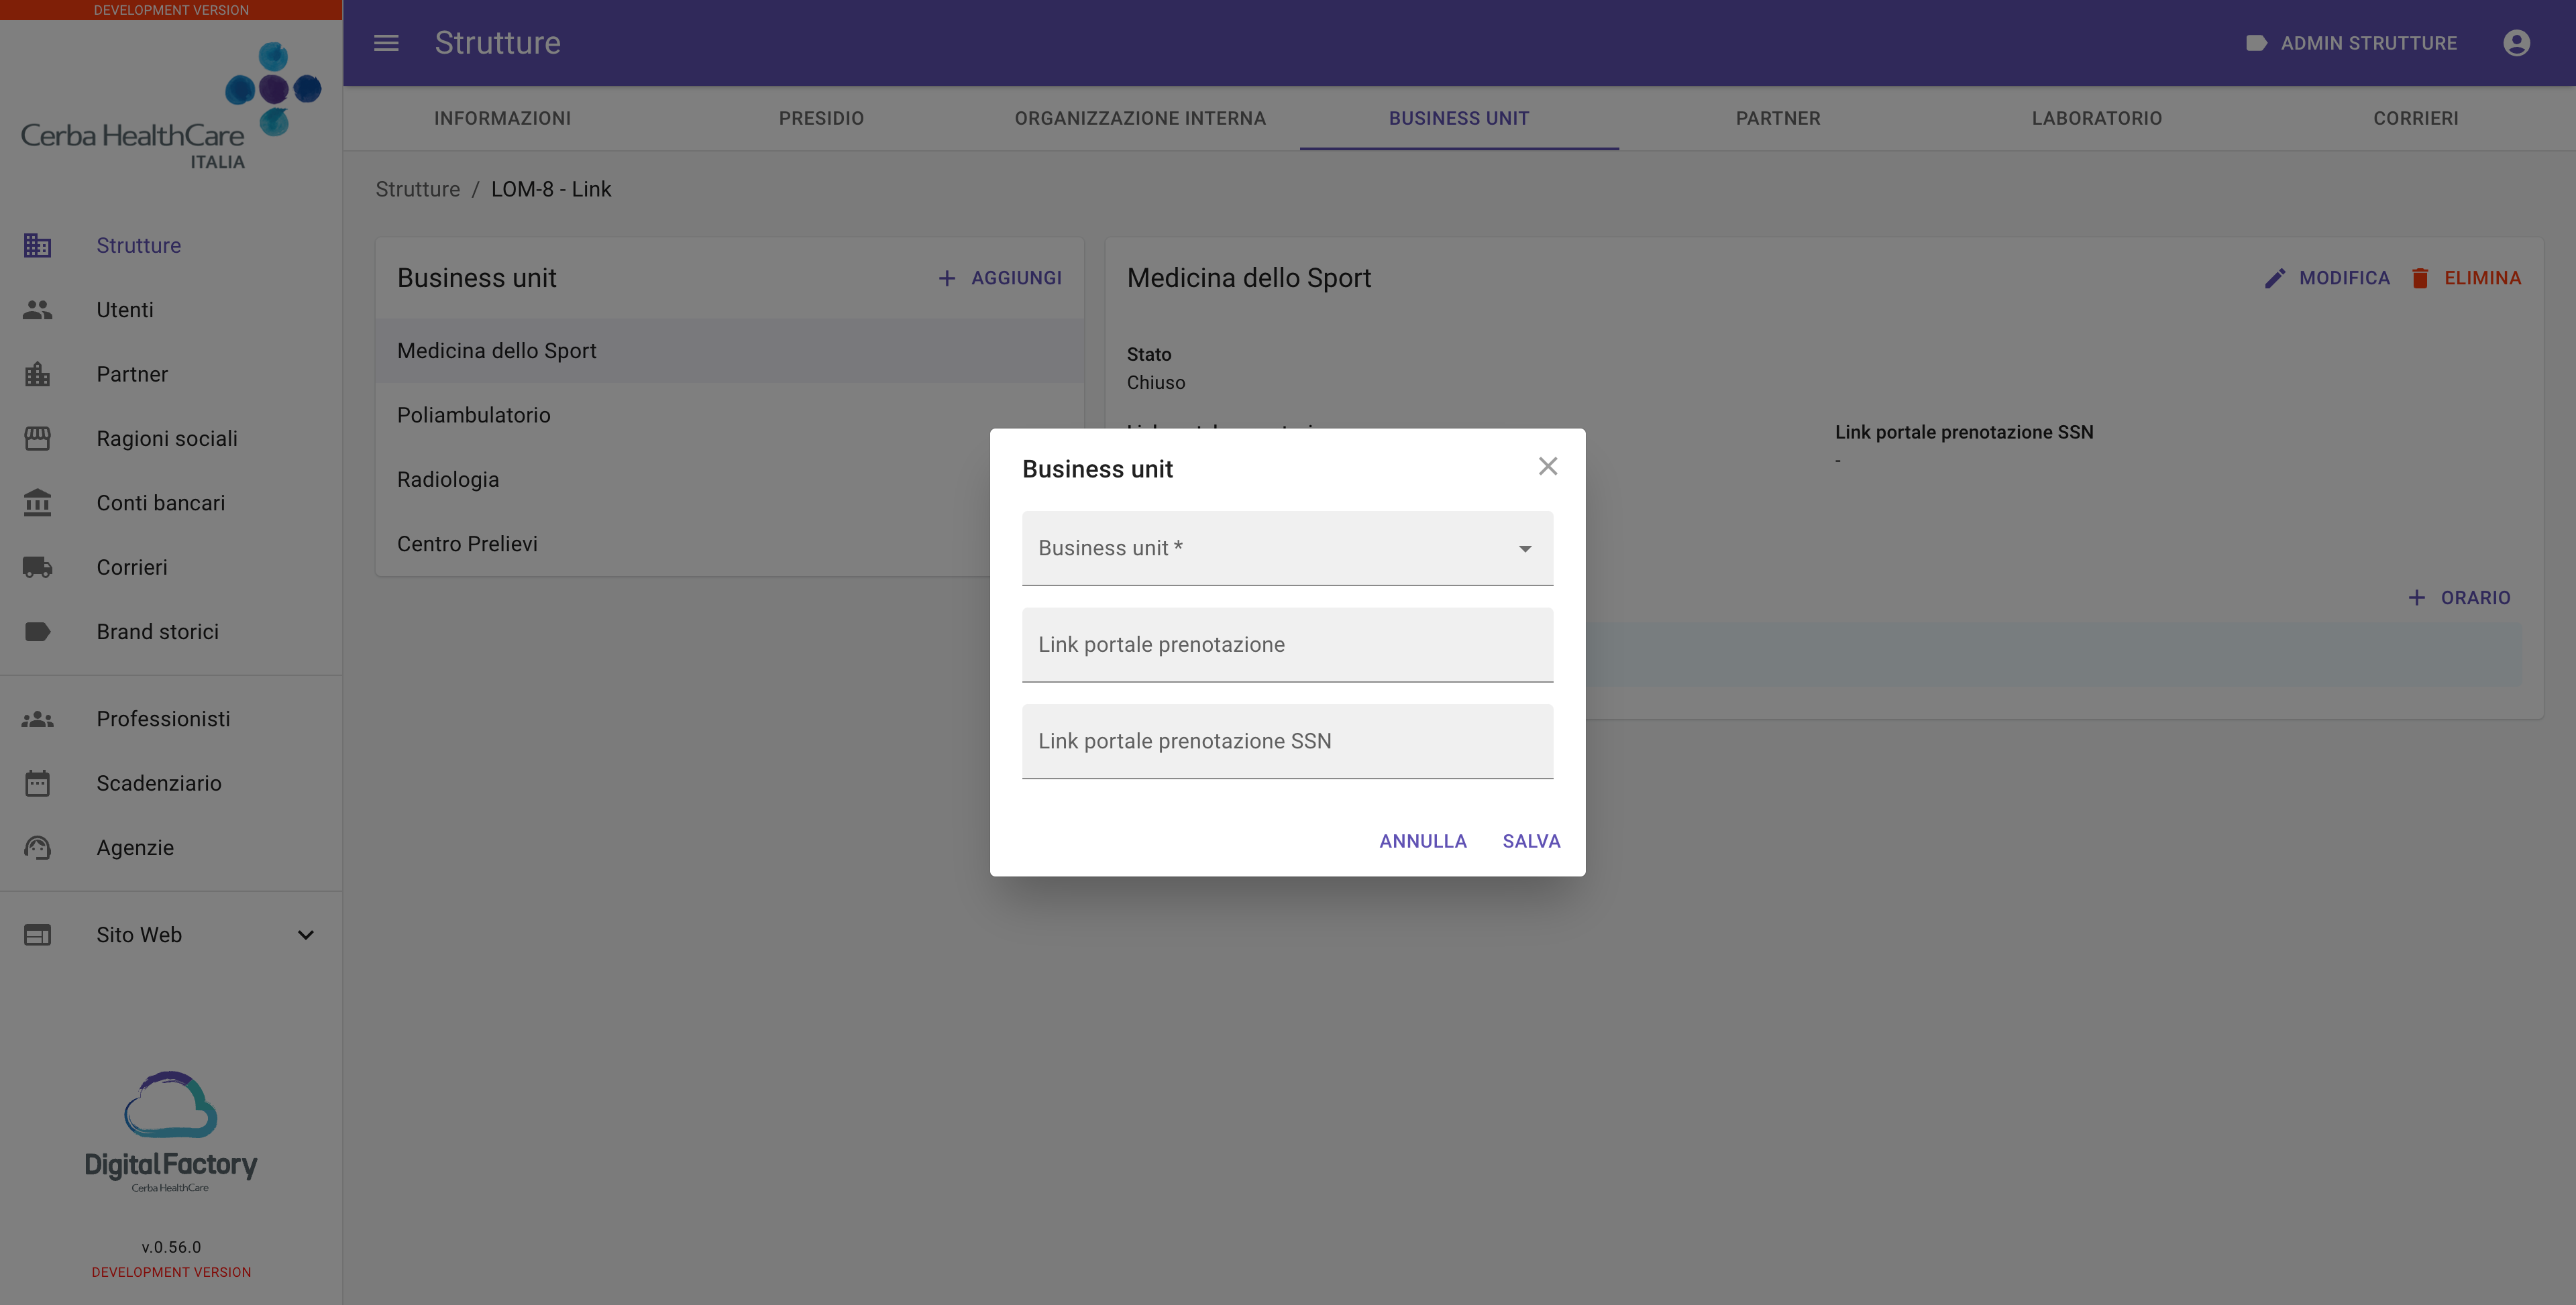
\includegraphics[width= 0.75\textwidth]{images/capitolo5/f1_f2_f3_websiteVisibility_email_links/ModalFacilityBusinessUnit_create.png} 
    \caption{Modale aggiunta nuova BU} 
    \label{fig:ModalFacilityBusinessUnit_create}
\end{figure}

\begin{figure}[H]
    \centering
    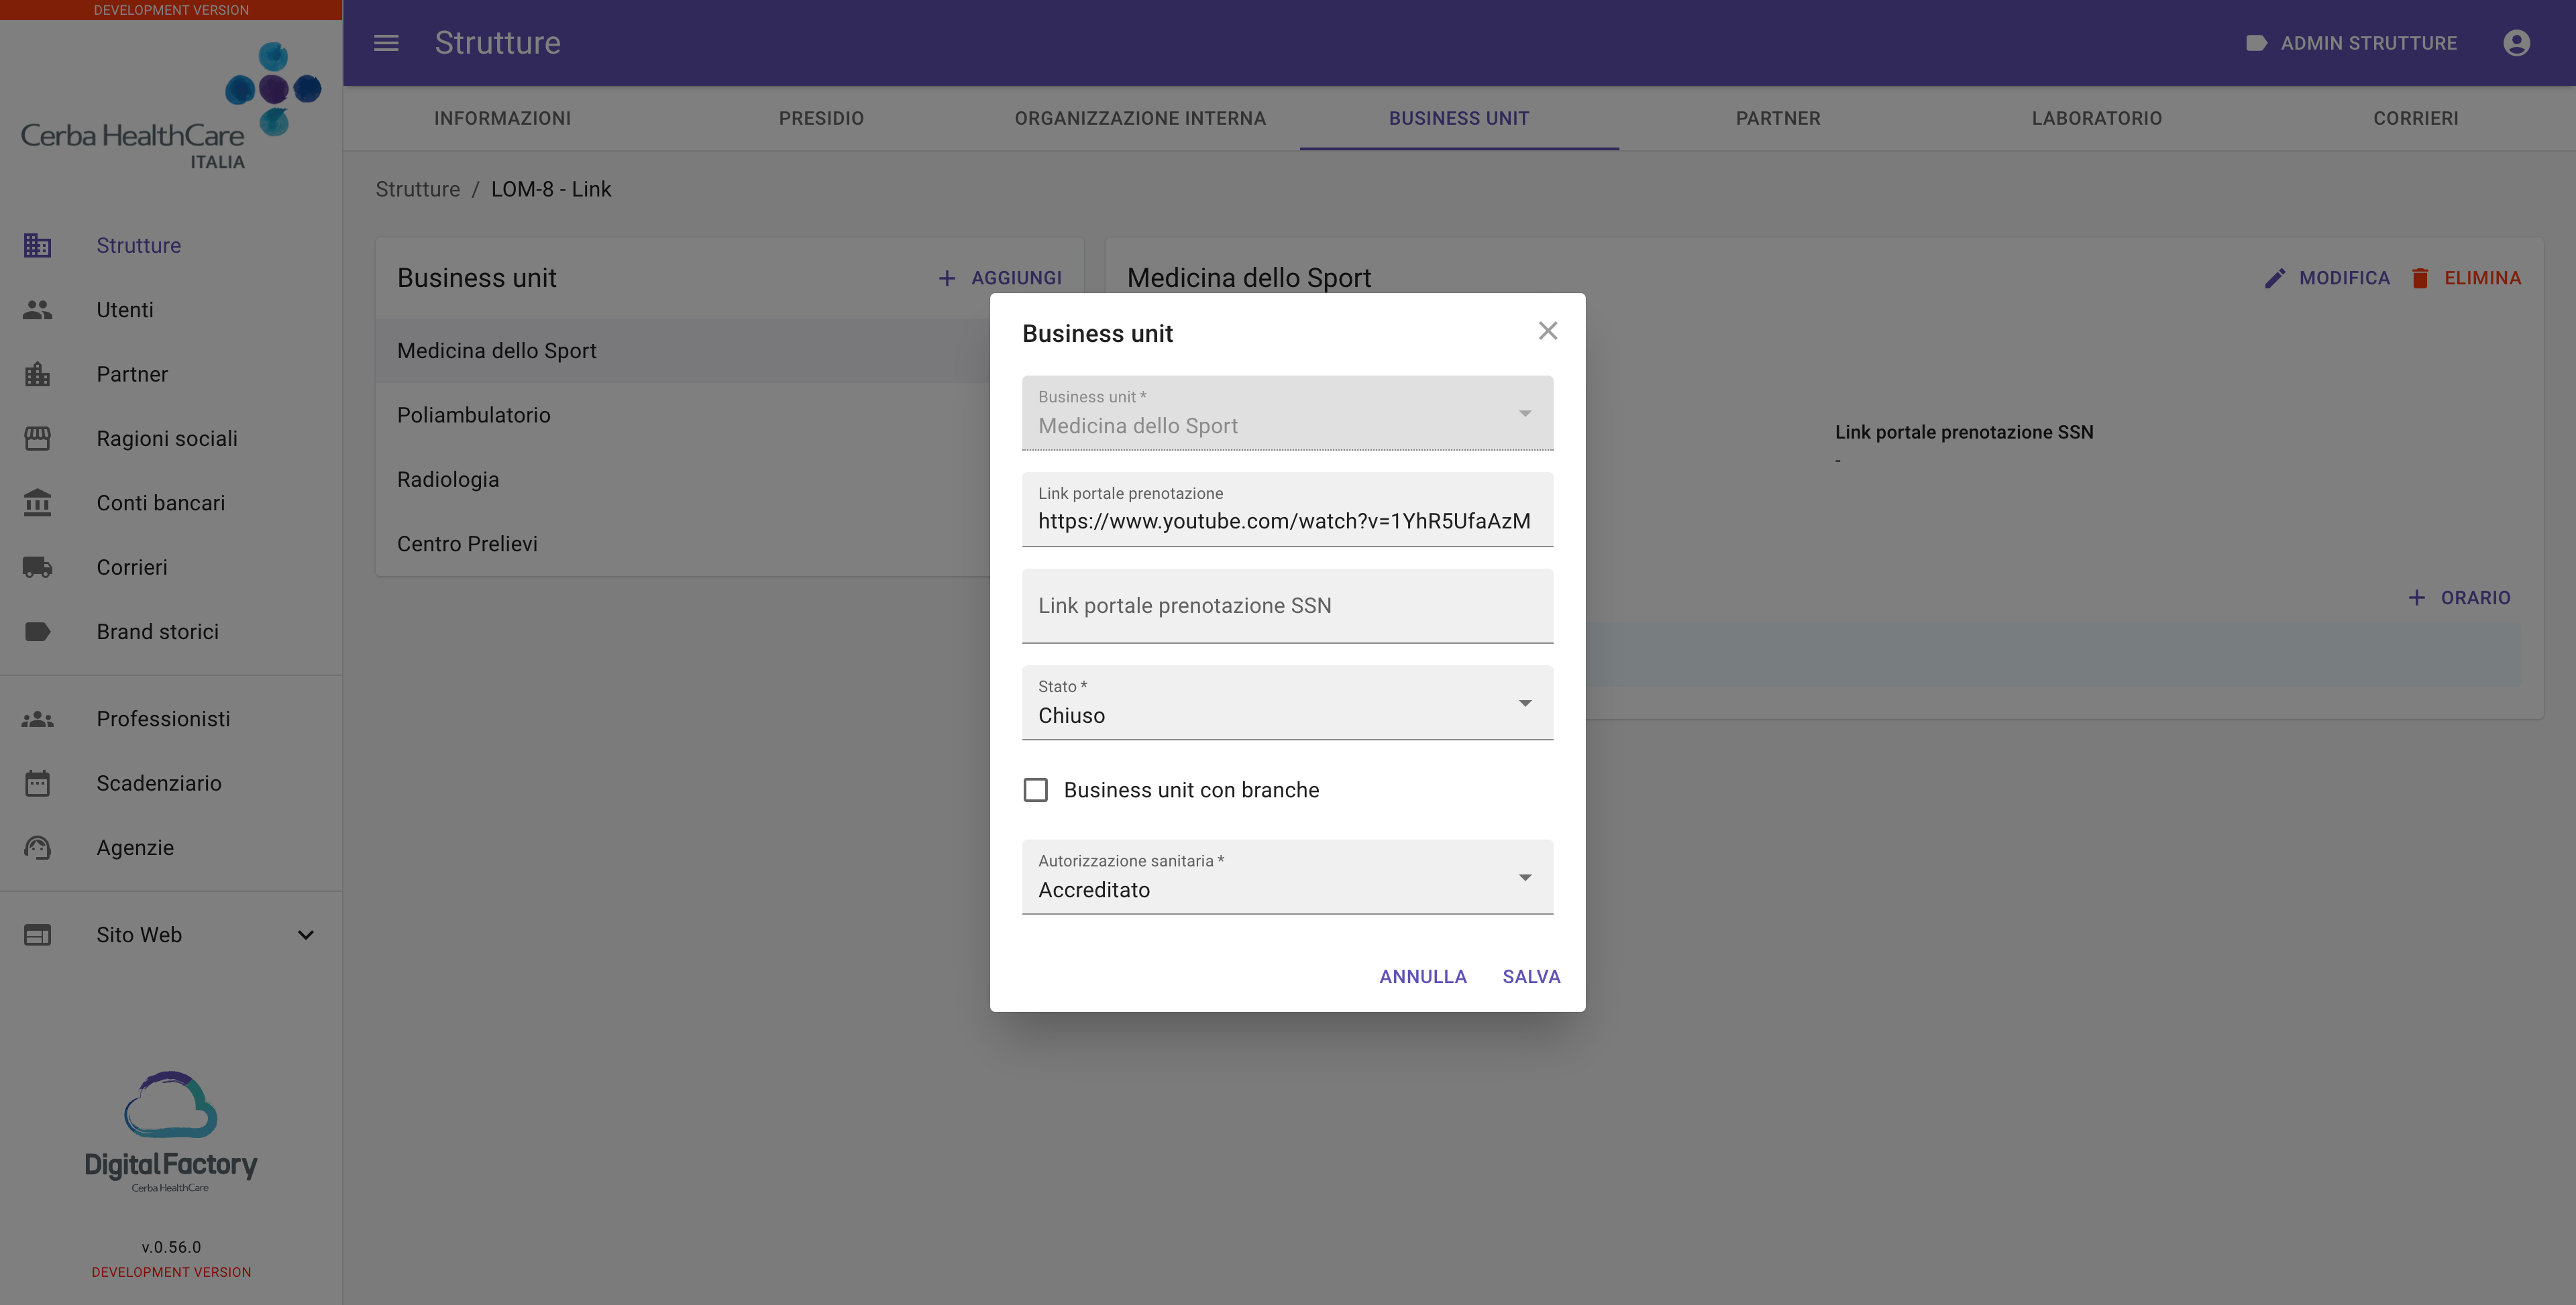
\includegraphics[width= 0.75\textwidth]{images/capitolo5/f1_f2_f3_websiteVisibility_email_links/ModalFacilityBusinessUnit_edit.png} 
    \caption{Modale modifica BU esistente} 
    \label{fig:ModalFacilityBusinessUnit_edit}
\end{figure}

\begin{figure}[H]
    \centering
    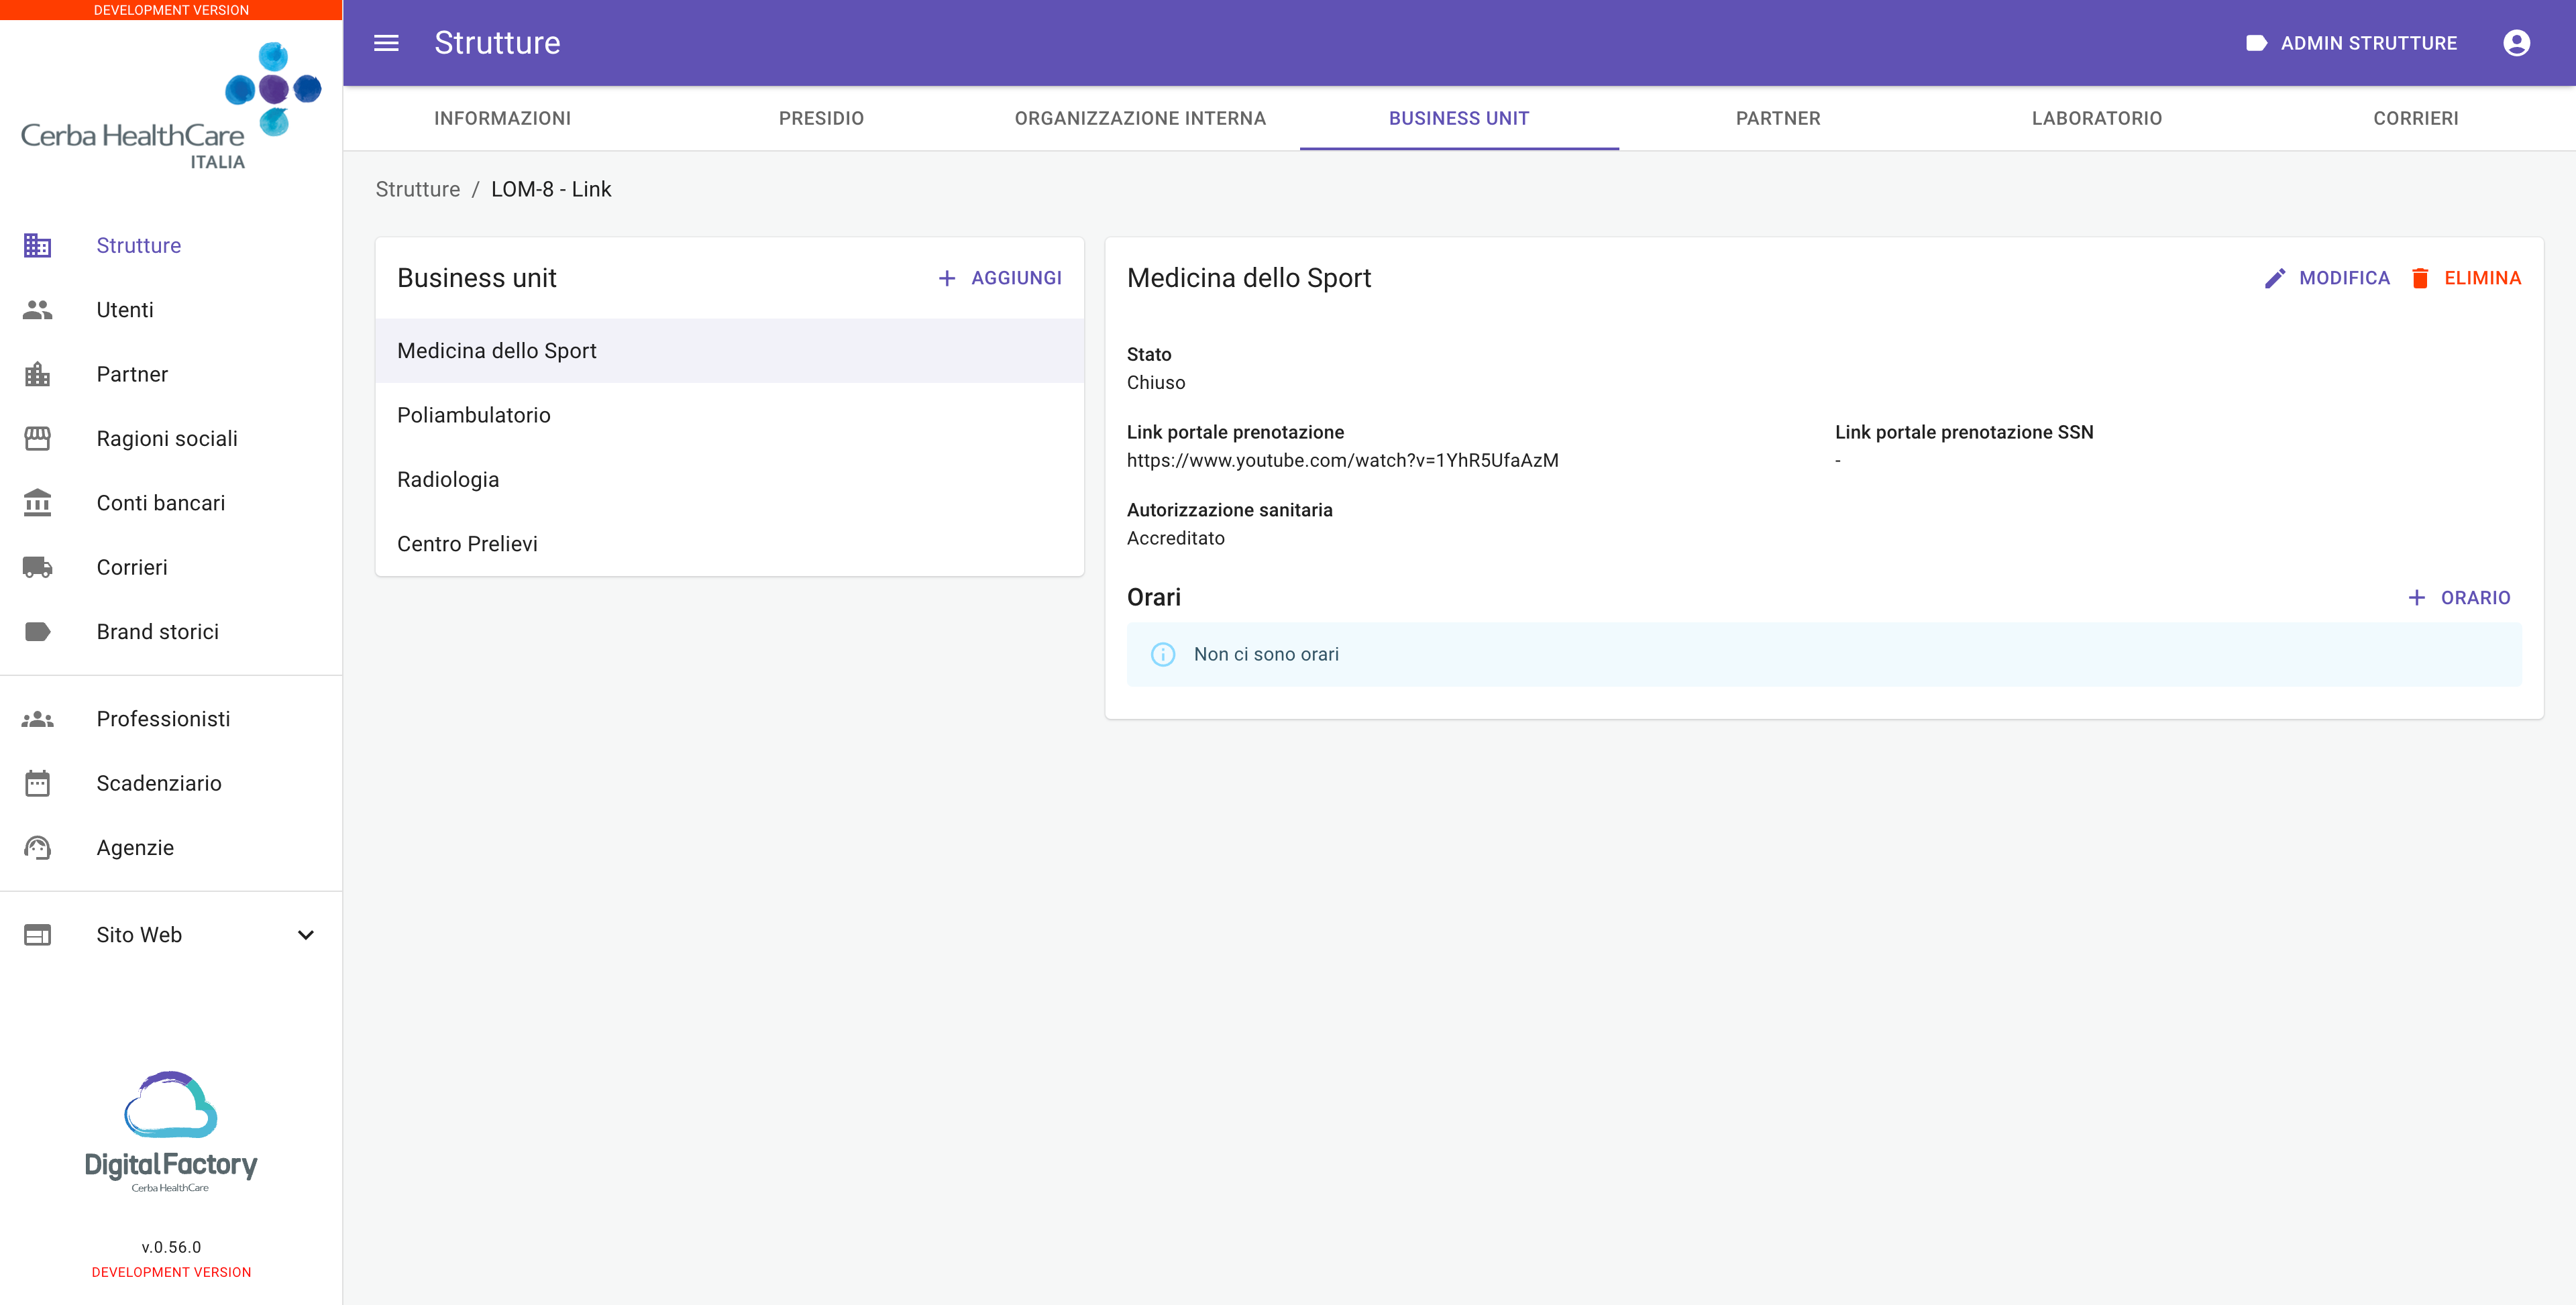
\includegraphics[width= 0.75\textwidth]{images/capitolo5/f1_f2_f3_websiteVisibility_email_links/TabBusinessUnit.png} 
    \caption{Tabella BU esistenti e tabella informazioni BU} 
    \label{fig:TabBusinessUnit}
\end{figure}

% ! PROBLEMA: ordine degli handler, alcuni nelle modali, altri nel componente
\newpage\section{F4: modifica tabella contratti di locazione}
\label{sec:F4: modifica tabella contratti di locazione}
\subparagraph{Requisiti}
La tabella dei contratti di locazione deve essere modificata in modo da poterne visualizzare e gestire di multipli.\\
Deve essere possibile aggiungere e archiviare contratti.\\
La tabella deve mostrare i contratti esistenti in una lista semplice e potersi espandere per mostrare i dettagli di ognuno.

\subparagraph{Procedura}
Il \textbf{primo passo} compiuto è consistito nell'esecuzione delle modifiche riguardanti il funzionamento delle modali. Poiché il codice preesistente permetteva già la modifica dei contratti di locazione esistenti, le introduzioni effettuate hanno riguardato la possibilità di aggiungerne di nuovi e la loro archiviazione.

\textit{In primis}, ciò ha necessitato la creazione delle funzioni \texttt{createRentalAgreement()} e \texttt{deleteRentalAgreement()}, le funzioni che effettuano le chiamate alle \gls{api} visibili nel \autoref{f4_api}. All'interno del loro corpo (alle righe 2 e 5) sono state utilizzate, rispettivamente, le funzioni \texttt{put()} e \texttt{del()}, funzioni che hanno il compito di effettuare richieste avvalendosi dei metodi \texttt{PUT} e \texttt{DELETE}.

\lstinputlisting[caption=Funzioni di chiamata \gls{api} contratti, label=f4_api, language=JSX]{listings/capitolo5/f4_rentalAgreement/api.js}

% ! rivedere
% def handler nel flusso
In secondo luogo, la gestione delle modali ha richiesto, a seconda dei casi, la creazione o l'aggiornamento degli \textit{handler}, le funzioni innescate al click di uno specifico bottone\footnote{Tendenzialmente, nel corpo degli \textit{handler} sono invocate le funzioni che effettuano le chiamate alle \gls{api}.}; questi possono essere divisi in due gruppi a seconda dell'obiettivo che si pongono.\\
Il primo ha come scopo l'apertura della modale ed è formato da \\\texttt{handleCreateRentalAgremment()} e \texttt{handleDeleteRentalAgreement()}, gli \textit{handler} mostrati nel \autoref{f4_RentalAgreement_handlers}, dichiarati all'interno del componente \texttt{RentalAgreement}. Il loro funzionamento è sostanzialmente identico e le operazioni che eseguono sono:
\begin{enumerate}
    \item L'impostazione dei dati della modale, attraverso l'uso del \textit{setter} \texttt{setData()} (alle righe 2 e 9);
    
    \item L'apertura della finestra di dialogo, con l'utilizzo della funzione \texttt{open()} (alle righe 3 e 10).
\end{enumerate}
Le differenze riguardano la modale con cui operano e i dati sui quali essa viene impostata. Infatti, se la funzione \texttt{handleCreateRentalAgreement()} ha a che fare con la finestra di dialogo \texttt{modalRentalAgreement}\footnote{La definizione della variabile della modale \texttt{modalRentalAgreement} non è riportata nel \autoref{f4_RentalAgreement_handlers} perché già parte del codice preesistente.} e ne imposta i dati su un oggetto vuoto, \\\texttt{handleDeleteRentalAgreement()} lavora invece con \texttt{modalConfirmDeleteRentalAgreement} e ne imposta i dati sull'oggetto \texttt{rentalAgreement}\footnote{La funzione \texttt{handleDeleteRentalAgreement()} si aspetta il parametro  \texttt{rentalAgreement} in \textit{input}. Per questo motivo, il valore di \texttt{rentalAgreement} corrisponde all'argomento fornito durante l'invocazione della funzione \texttt{handleDeleteRentalAgreement()}.}.
L'oggetto di quest'ultima finestra di dialogo è stato definito attraverso l'uso dell'\textit{hook} \texttt{useModal()} (a riga 6).

\lstinputlisting[caption=\textit{Handler} apertura modale, label=f4_RentalAgreement_handlers, language=JSX]{listings/capitolo5/f4_rentalAgreement/RentalAgreement_handlers.js}
% spazio
Il secondo gruppo di \textit{handler} ha invece come obiettivo l'effettiva manipolazione dei dati ed è formato da \texttt{handleSaveAgreement()} e \texttt{handleArchiveConfirmRentalAgreement()}.\\
Entrambe le funzioni adempiono al loro compito invocando, all'interno del loro corpo, una delle funzioni di chiamata alle \acrshort{api} definite poco fa.\\
Da un lato, come mostrato nel \autoref{f4_ModalRentalAgreement_handleSaveAgreement}, l'\textit{handler} \texttt{handleSaveAgreement()} (già esistente all'interno del componente \texttt{ModalRentalAgreement} in passato) è stato aggiornato con l'introduzione della possibilità di aggiungere un nuovo contratto di locazione. La già esistente riga di codice atta alla gestione della modifica dei contratti, infatti, è stata resa parte di una condizione che si avvale della sintassi \texttt{if...else} (da riga 3 a 7) per esprimere il seguente concetto: se è presente la proprietà \texttt{uuid} dell'oggetto \texttt{rentalAgreement} esegui la funzione \texttt{editRentalAgreement()} passandole come parametri la proprietà \texttt{uuid} stessa e la variabile \texttt{body}; in caso contrario esegui la funzione \texttt{createRentalAgreement()} passandole come parametri le variabili \texttt{uuidFacility} e \texttt{body}.\\
In altre parole, se esiste un contratto di locazione eseguine la modifica, altrimenti creane uno nuovo.

\lstinputlisting[caption=\textit{Handler} aggiunta nuovo contratto, label=f4_ModalRentalAgreement_handleSaveAgreement, language=JSX]{listings/capitolo5/f4_rentalAgreement/ModalRentalAgreement_handleSaveAgreement.js}
% spazio
Dall'altro lato, come illustrato nel \autoref{f4_RentalAgreement_handleArchiveConfirmRentalAgreement}, è stato creato, di nuovo all'interno del componente \texttt{RentalAgreement}, l'\textit{handler} \texttt{handleArchiveConfirmRentalAgreement()} per l'archiviazione dei contratti di locazione. Questo esegue l'archiviazione del contratto, grazie alla funzione \texttt{deleteRentalAgreement()}, e l'aggiornamento della lista dei contratti di locazione, tramite \texttt{fetchRentalAgreements()}.

\lstinputlisting[caption=\textit{Handler} archiviazione contratto, label=f4_RentalAgreement_handleArchiveConfirmRentalAgreement, language=JSX]{listings/capitolo5/f4_rentalAgreement/RentalAgreement_handleArchiveConfirmRentalAgreement.js}

Il \textbf{secondo passo} compiuto, invece, è consistito nell'aggiornamento della \acrshort{ui} del componente \texttt{RentalAgreement}, elemento responsabile dell'intera tabella dei contratti di locazione.

Come possibile vedere nel \autoref{f4_RentalAgreement_UI}, un componente \texttt{Card} (da riga 2 a 28) è stato utilizzato per racchiudere tutti i componenti figli che formano la struttura della tabella.\\
\texttt{CardHeader}, il primo di essi, ha come compito il \textit{rendering} dell'\textit{header} e le sue \textit{props} sono: 
\begin{itemize}
    \item \texttt{subheader} (a riga 4): il suo valore è la stringa \texttt{"Contratti locazione"};
    \item \texttt{action} (da riga 5 a 12): il suo valore è il componente \texttt{Button}, il quale racchiude il testo “Aggiungi” ed è dotato, a sua volta, delle \textit{props}:
        \begin{itemize}
            \item \texttt{onClick}: il suo valore è l'\textit{handler} \texttt{handleCreateRentalAgreement};
            \item \texttt{startIcon}: il suo valore è il componente \texttt{AddIcon}.
        \end{itemize}
\end{itemize}
Il secondo componente figlio di \texttt{Card} è \texttt{Divider} (a riga 15), elemento che stabilisce un confine fra l'\textit{header} e tutto ciò che sta al di sotto di lui.\\
La struttura di \texttt{Card} termina con il componente \texttt{Table}, terzo ed ultimo elemento che si occupa del \textit{rendering} del corpo della tabella (da riga 18 a 29). Questo racchiude un componente \texttt{TableBody} all'interno del quale viene effettuato un \textit{mapping}: l'iteratore \texttt{map()} è utilizzato sull'\textit{array} \texttt{rentalAgreements} affinché tutti gli oggetti che lo compongono vengano visualizzati grazie all'istanza del componente \texttt{TabBuildingRentalAgreementTable}. Le \textit{props} passate a quest'ultima sono: 
\begin{itemize}
    \item \texttt{key}: il suo valore è la proprietà \texttt{uuid} dell'oggetto \texttt{el};
    
    \item \texttt{el}: il singolo contratto che, di volta in volta, viene mappato sul componente. Il suo valore è l'oggetto \texttt{el};
    
    \item \texttt{handleEditRentalAgreement}: il suo valore è l'\textit{handler} \texttt{handleEditRentalAgreement()};
    
    \item \texttt{handleDeleteRentalAgreement}: il suo valore è l'\textit{handler} \texttt{handleDeleteRentalAgreement()}.
\end{itemize}
Le ultime due \textit{props} forniscono le funzioni invocate dai bottoni contenuti nel componente.

Inoltre, è stato necessario introdurre il componente \texttt{ModalConfirm}, elemento responsabile della restituzione dell'ulteriore finestra di dialogo che compare per chiedere all'utente la conferma prima di eseguire l'archiviazione di un contratto.\\
Tramite una condizione che si avvale dell'operatore logico AND (da riga 32 a 39) viene stabilito che, se il valore della proprietà \texttt{isOpen} dell'oggetto \\\texttt{modalConfirmDeleteRentalAgreement} è vero, allora viene eseguito il \textit{rendering} del componente. In tal caso, le \textit{props} fornite a \texttt{ModalConfirm} sono: 
\begin{itemize}
    \item \texttt{modal}: il suo valore è l'oggetto \texttt{modalConfirmDeleteRentalAgreement};
    \item \texttt{title}: il suo valore è la stringa \texttt{'Archivia contratto locazione'};
    \item \texttt{text}: il suo valore è un'espressione che stabilisce la composizione di una stringa; 
    \item \texttt{handleConfirm}: il suo valore è l'\textit{handler} \texttt{handleArchiveConfirmRentalAgreement()}.
\end{itemize}
La funzione passata alla \textit{prop} \texttt{handleConfirm} è quella che viene invocata dal bottone del componente.

\lstinputlisting[caption=Tabella contratti esistenti, label=f4_RentalAgreement_UI, language=JSX]{listings/capitolo5/f4_rentalAgreement/RentalAgreement_UI.js}

Il \textbf{terzo passo} è consistito nella gestione del corpo della tabella per la visualizzazione delle informazioni dei contratti di locazione. 
Ciò è stato fatto attraverso l'implementazione di un nuovo componente creato \textit{ad hoc}, \texttt{TabBuildingRentalAgreementTable}, del quale era stata utilizzata precedentemente l'istanza all'interno del \textit{mapping}.\\
Come prassi vuole, la definizione di tale elemento ha previsto l'importazione delle \textit{props} passate alla sua istanza; il \autoref{f4_TabBuildingRentalAgreementTable_component} mostra che ciò è stato fatto, attraverso la tecnica della destrutturazione, per \texttt{el}, \texttt{handleEditRentalAgreement()} e \texttt{handleDeleteRentalAgreement()} (a riga 2).

\lstinputlisting[caption=Componente \texttt{TabBuildingRentalAgreementTable}, label=f4_TabBuildingRentalAgreementTable_component, language=JSX]{listings/capitolo5/f4_rentalAgreement/TabBuildingRentalAgreementTable_component.js}

Anche in questo caso, delle modifiche a livello di logica hanno costituito lo \textit{step} iniziale. Poiché fra i requisiti era presente l'espandibilità di ogni riga della tabella, la definizione del componente è stata seguita dalla gestione di questa dinamica\footnote{La gestione della dinamica di espansione è stata effettuata all'interno del corpo del componente \texttt{TabBuildingRentalAgreementTable}.}, che viene illustrara nel \autoref{f4_TabBuildingRentalAgreementTable_dynamic}.\\
Il concetto di espansione è stato implementato grazie alla variabile di stato \texttt{toggleOpen} e al relativo \textit{setter} \texttt{setToggleOpen()}, dichiarati attraverso l'\textit{hook} \texttt{useState()} (a riga 1). Poiché, salvo click da parte dell'utente, le righe della tabella appaiono nella pagina come non espanse, \texttt{toggleOpen} è stata inizializzata con il valore booleano \texttt{false}.\\
Inoltre, è possibile vedere l'\textit{handler} \texttt{handleOpenRentalAgreement}, la funzione responsabile del funzionamento del meccanismo di espansione. Questa sfrutta il \textit{setter} \texttt{setToggleOpen()} per sostituire il precedente valore della variabile di stato \texttt{toggleOpen} con il suo opposto ogni volta che viene invocata.

\lstinputlisting[caption=Dinamica apertura riga tabella contratti, label=f4_TabBuildingRentalAgreementTable_dynamic, language=JSX]{listings/capitolo5/f4_rentalAgreement/TabBuildingRentalAgreementTable_dynamic.js}

Il \textbf{quarto} e \textbf{ultimo} passo è consistito nella creazione della \acrshort{ui} del neonato componente \texttt{TabBuildingRentalAgreementTable}.

Il \autoref{f4_TabBuildingRentalAgreementTable_UI} mostra come il tag padre \texttt{<>} sia stato utilizzato come contenitore per due grandi componenti figli \texttt{TableRow}. Questi costituiscono le due righe che, di volta in volta, racchiudono le informazioni dei contratti di locazione esistenti. Se la prima deve permettere all'utente di visualizzare, anche senza l'espansione della riga, solo alcuni dati del contratto e i bottoni per la sua gestione, la seconda deve invece mostrare, una volta espansa la riga, tutte le informazioni del contratto nel dettaglio.\\
Entrambi i componenti \texttt{TableRow} contengono, a loro volta, molti elementi figli; all'interno del primo (da riga 2 a 41) sono presenti quattro componenti \texttt{TableCell}:
\begin{itemize}
    \item \texttt{TableCell} (da riga 3 a 7): contiene il componente \texttt{Typography} che effettua il \textit{rendering} di un sottotitolo. Il sottotitolo ritornato è quello risultante dalla condizione che si avvale dell'operatore ternario (a riga 5); questa esprime il seguente concetto: se la proprietà \texttt{label} dell'oggetto \texttt{type} (contenuto dall'oggetto \texttt{el}) è vera, allora restituisci tale proprietà, altrimenti una stringa dal valore \texttt{'-'};
    
    \item \texttt{TableCell} (a riga 9): contiene una condizione che si avvale dell'operatore logico AND per esprimere il seguente concetto: solo se la proprietà \texttt{archived} dell'oggetto \texttt{el} è vera, restituisci la stringa \texttt{'(archiviato)'};
    
    \item \texttt{TableCell} (da riga 11 a 25): contiene il componente \texttt{Button}, il bottone necessario all'espansione della riga. Le su \textit{props} più importanti sono:
    \begin{itemize}
        \item \texttt{onClick} (a riga 14): il suo valore è \texttt{handleOpenRentalAgreement()};
        
        \item \texttt{startIcon} (a riga 15): il suo valore è una condizione che si avvale dell'operatore ternario per esprimere il seguente concetto: se la variabile di stato \texttt{toggleOpen} ha come valore il \texttt{true}, restituisci il componente \texttt{KeyBoardArrowUpIcon}, altrimenti \texttt{KeyBoardArrowDownIcon}. In altre parole, se la riga è espansa restituisci una freccia che punta verso l'alto, altrimenti, una freccia che punta verso il basso.\\
        All'interno del componente viene effettuato il \textit{rendering} del testo “Mostra”;
    \end{itemize}

    \item \texttt{TableCell} (da riga 27 a 40): contiene due componenti \texttt{IconButton}, ovvero i bottoni atti alla manipolazione dei contratti di locazione. Entrambi sono dotati della \textit{prop} \texttt{onClick}, il cui valore è però diverso a seconda della casistica: quello del bottone che si occupa della modifica è l'\textit{handler} \texttt{handleEditRentalAgreement()}, mentre quello del bottone atto all'archiviazione è \texttt{handleDeleteRentalAgreement()}. A entrambe le funzioni viene passato come argomento l'oggetto \texttt{el}, il contratto che di volta in volta sarà modificato o archiviato.\\
    Inoltre, il bottone per la modifica contiene il componente \texttt{EditIcon}, mentre quello per l'archiviazione \texttt{DeleteIcon}.
\end{itemize}
% spazio
All'interno del secondo componente \texttt{TableRow} (da riga 43 a 60) è invece presente un solo \texttt{TableCell} che contiene a sua volta il componente \texttt{Collapse} (da riga 45 a 58), elemento il cui compito è l'effettiva gestione della dinamica di apertura e chiusura della riga della tabella; ciò avviene grazie alla \textit{prop} \texttt{in}, il cui valore è la variabile di stato \texttt{toggleOpen}.

Le informazioni dettagliate di ogni contratto di locazione vengono mostrate attraverso un'ulteriore tabella, visibile solamente a riga espansa, contenuta dal componente \texttt{TableBody}\footnote{La struttura della tabella, incomincia in realtà con il componente \texttt{TableContainer} (da riga 46 a 57).}. Questo è composto da tanti componenti \texttt{TableRow} quante sono le proprietà dell'oggetto \texttt{el}, ovvero, quante sono le informazioni del contratto che si desidera vengano mostrate all'interno della tabella. Ogni riga è formata a sua volta da due componenti \texttt{TableCell}, una cella per la visualizzazione del tipo di informazione riportata, e una per il dato associato al tipo di informazione. 

\lstinputlisting[caption=Riga tabella contratti, label=f4_TabBuildingRentalAgreementTable_UI, language=JSX]{listings/capitolo5/f4_rentalAgreement/TabBuildingRentalAgreementTable_UI.js}

\paragraph{\textit{Output} grafico}
\begin{figure}[H]
    \centering
    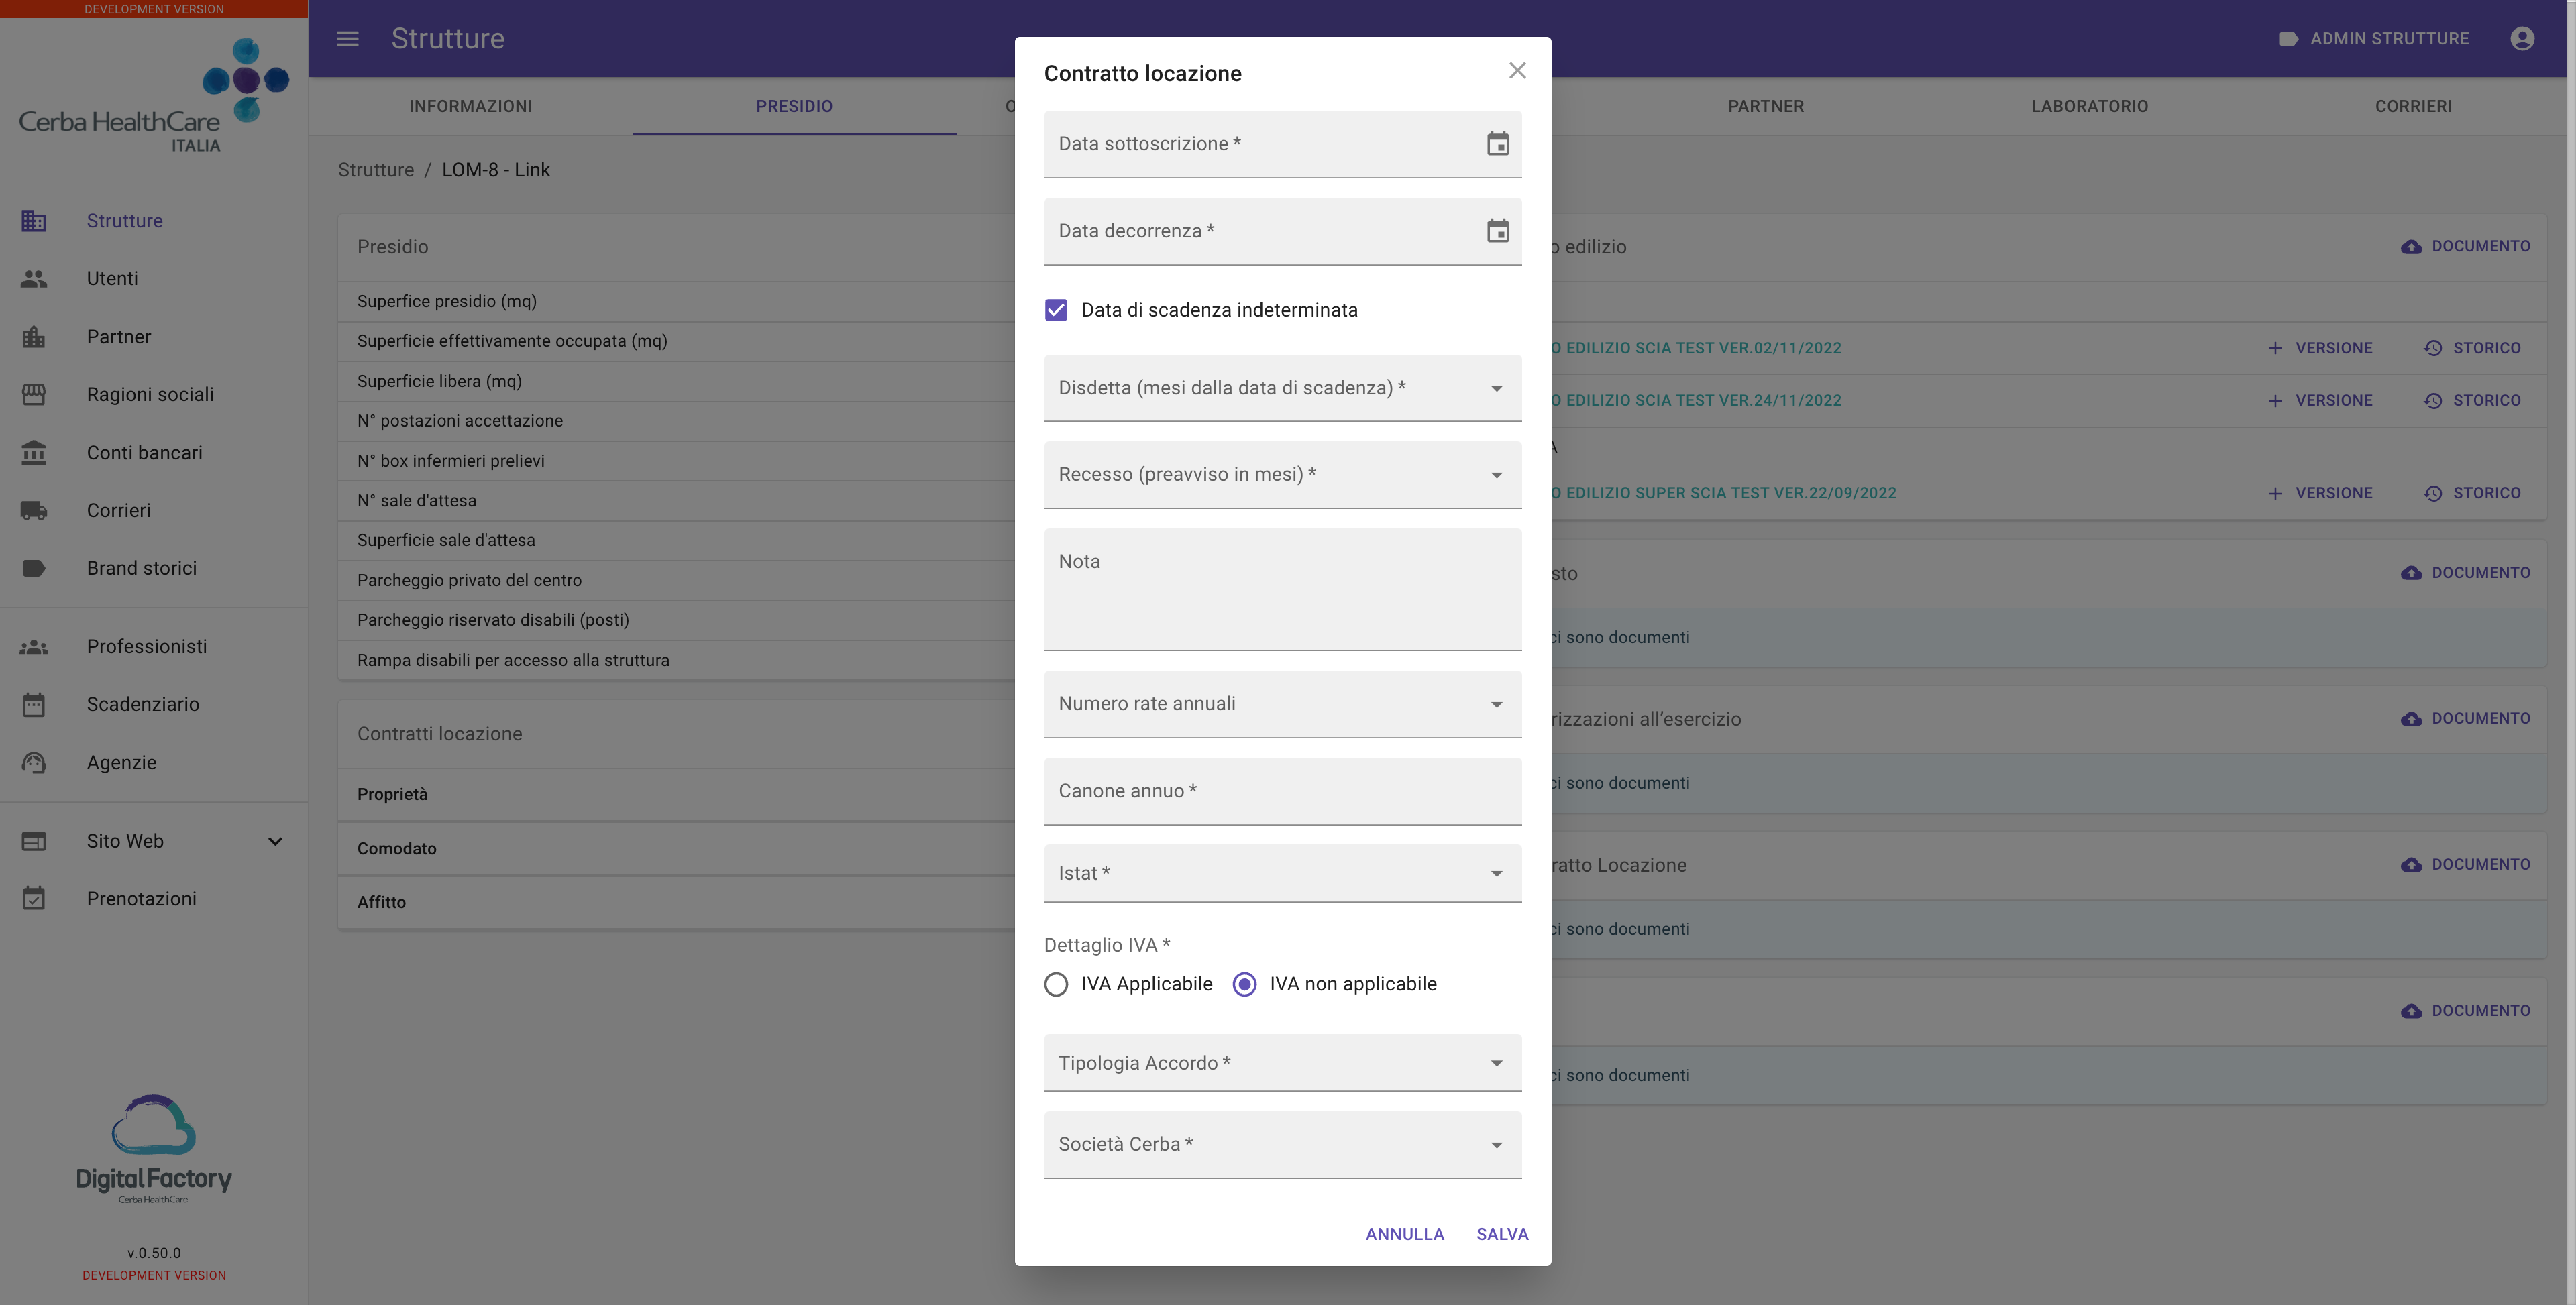
\includegraphics[width=0.75\textwidth]{images/capitolo5/f4_rentalAgreement/RentalAgreement_create.png} 
    \caption{Modale aggiunta nuovo contratto} 
    \label{fig:RentalAgreement_create}
\end{figure}

\begin{figure}[H]
    \centering
    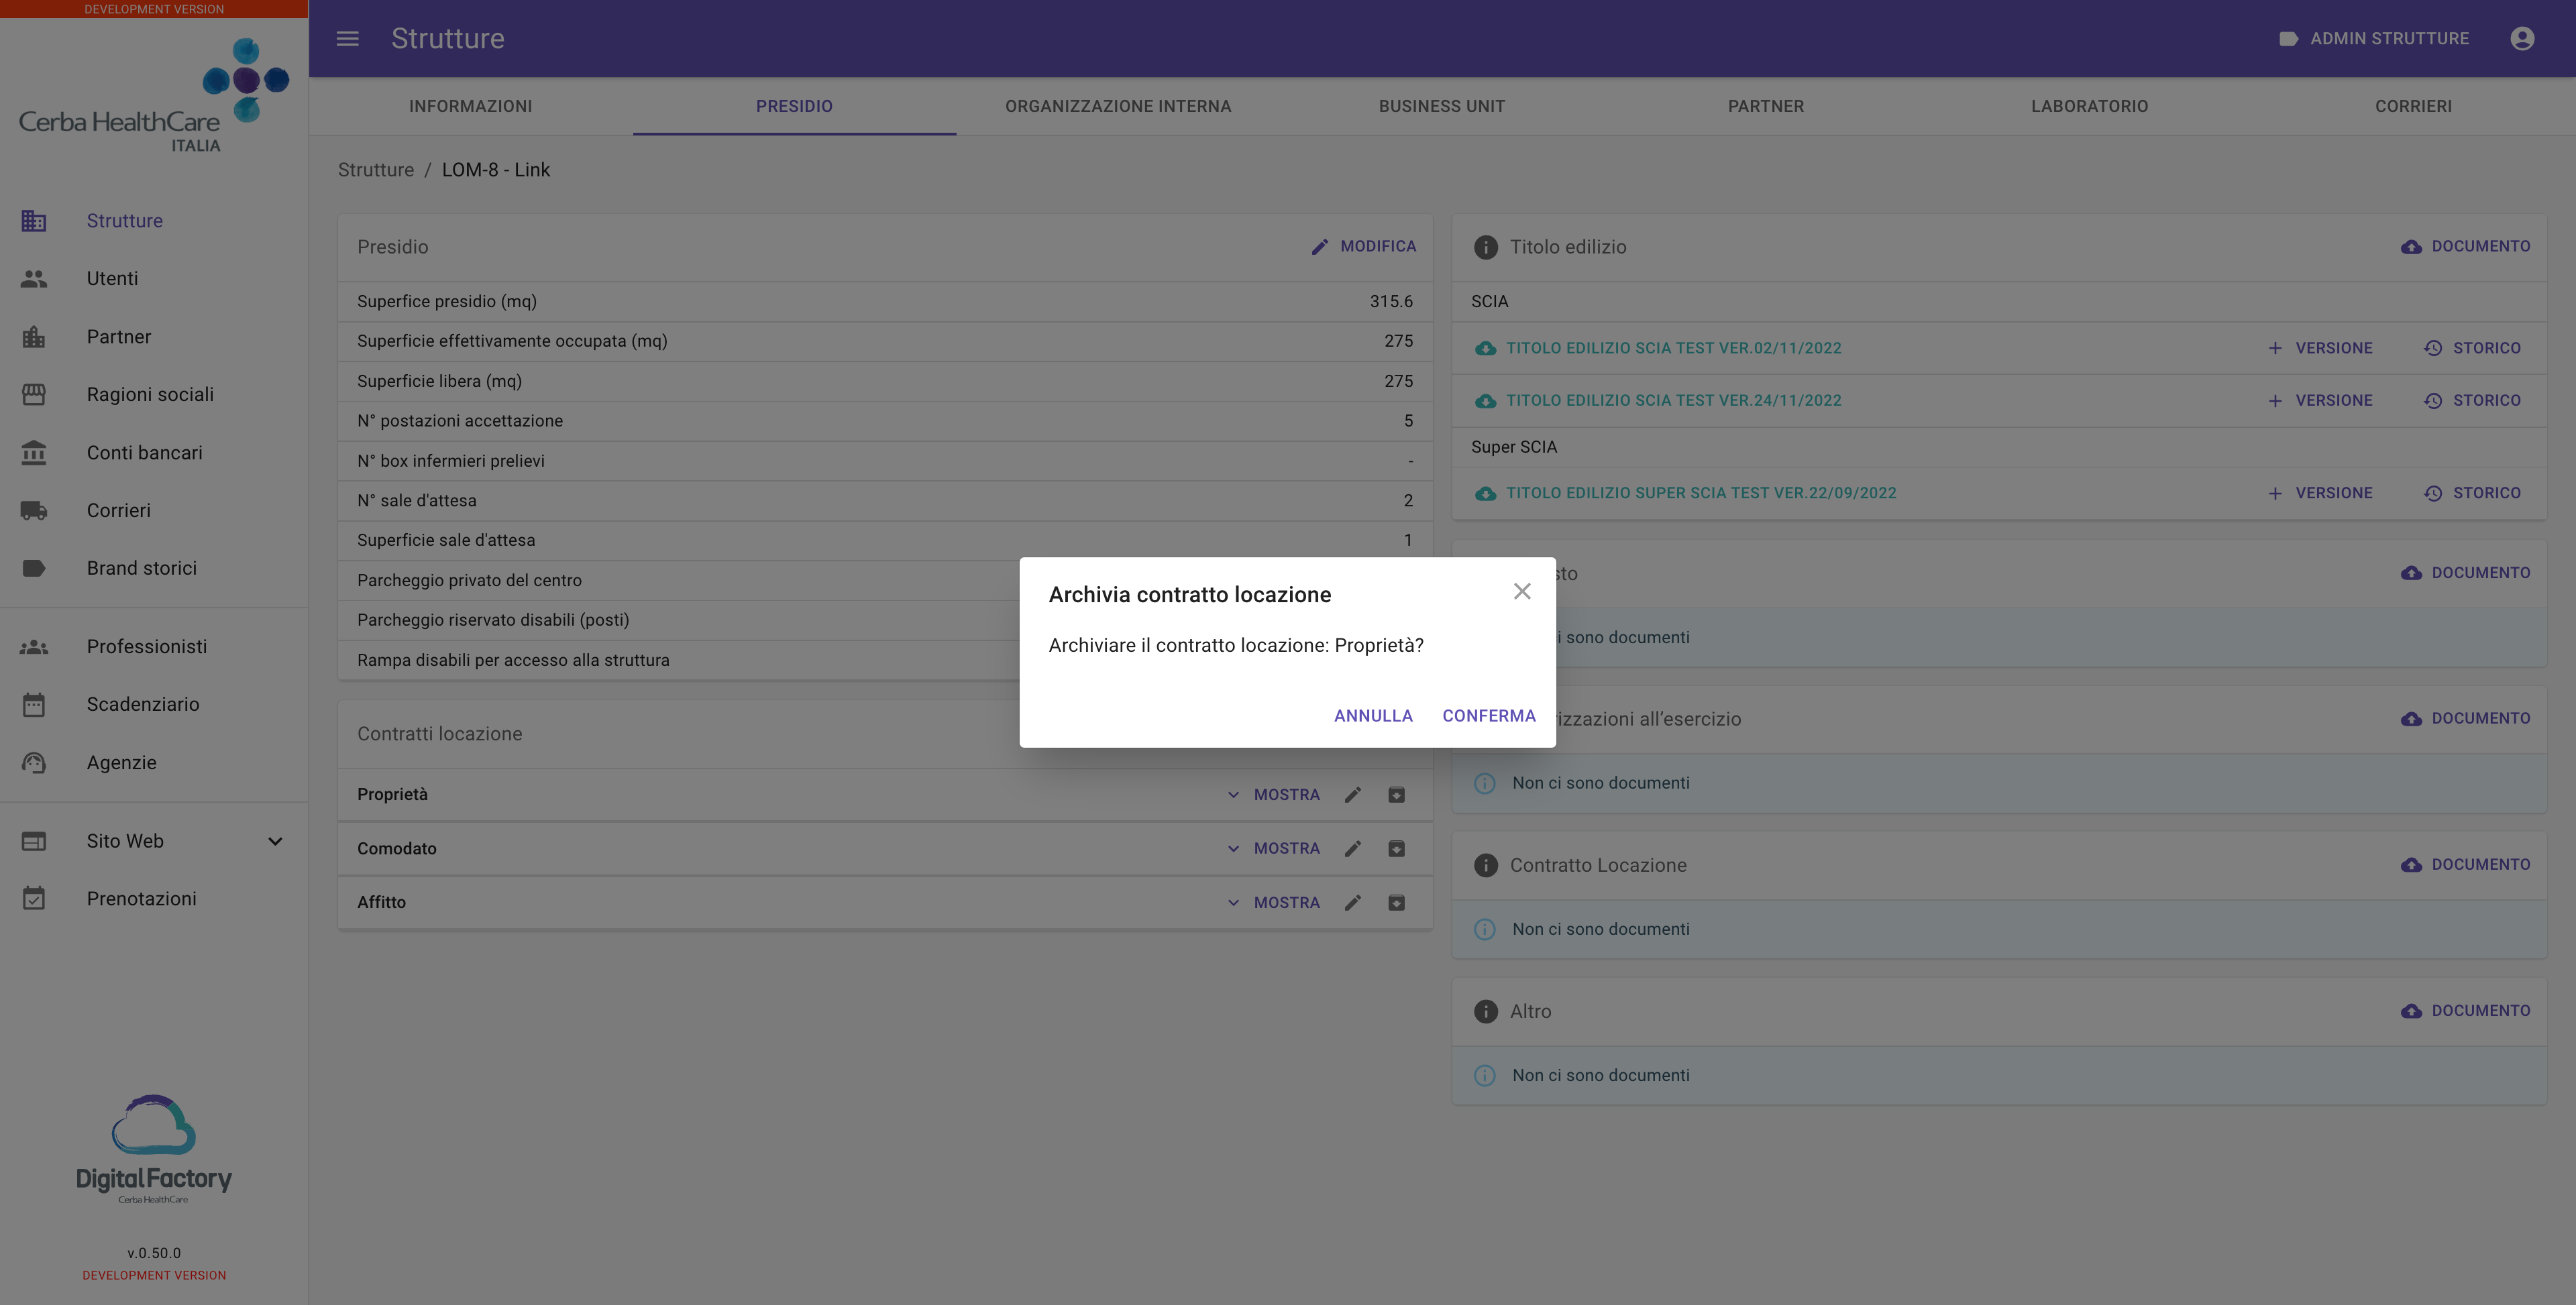
\includegraphics[width=0.75\textwidth]{images/capitolo5/f4_rentalAgreement/ModalRentalAgreement_archive.png} 
    \caption{Modale archiviazione contratto esistente} 
    \label{fig:ModalRentalAgreement_archive}
\end{figure}

\begin{figure}[H]
    \centering
    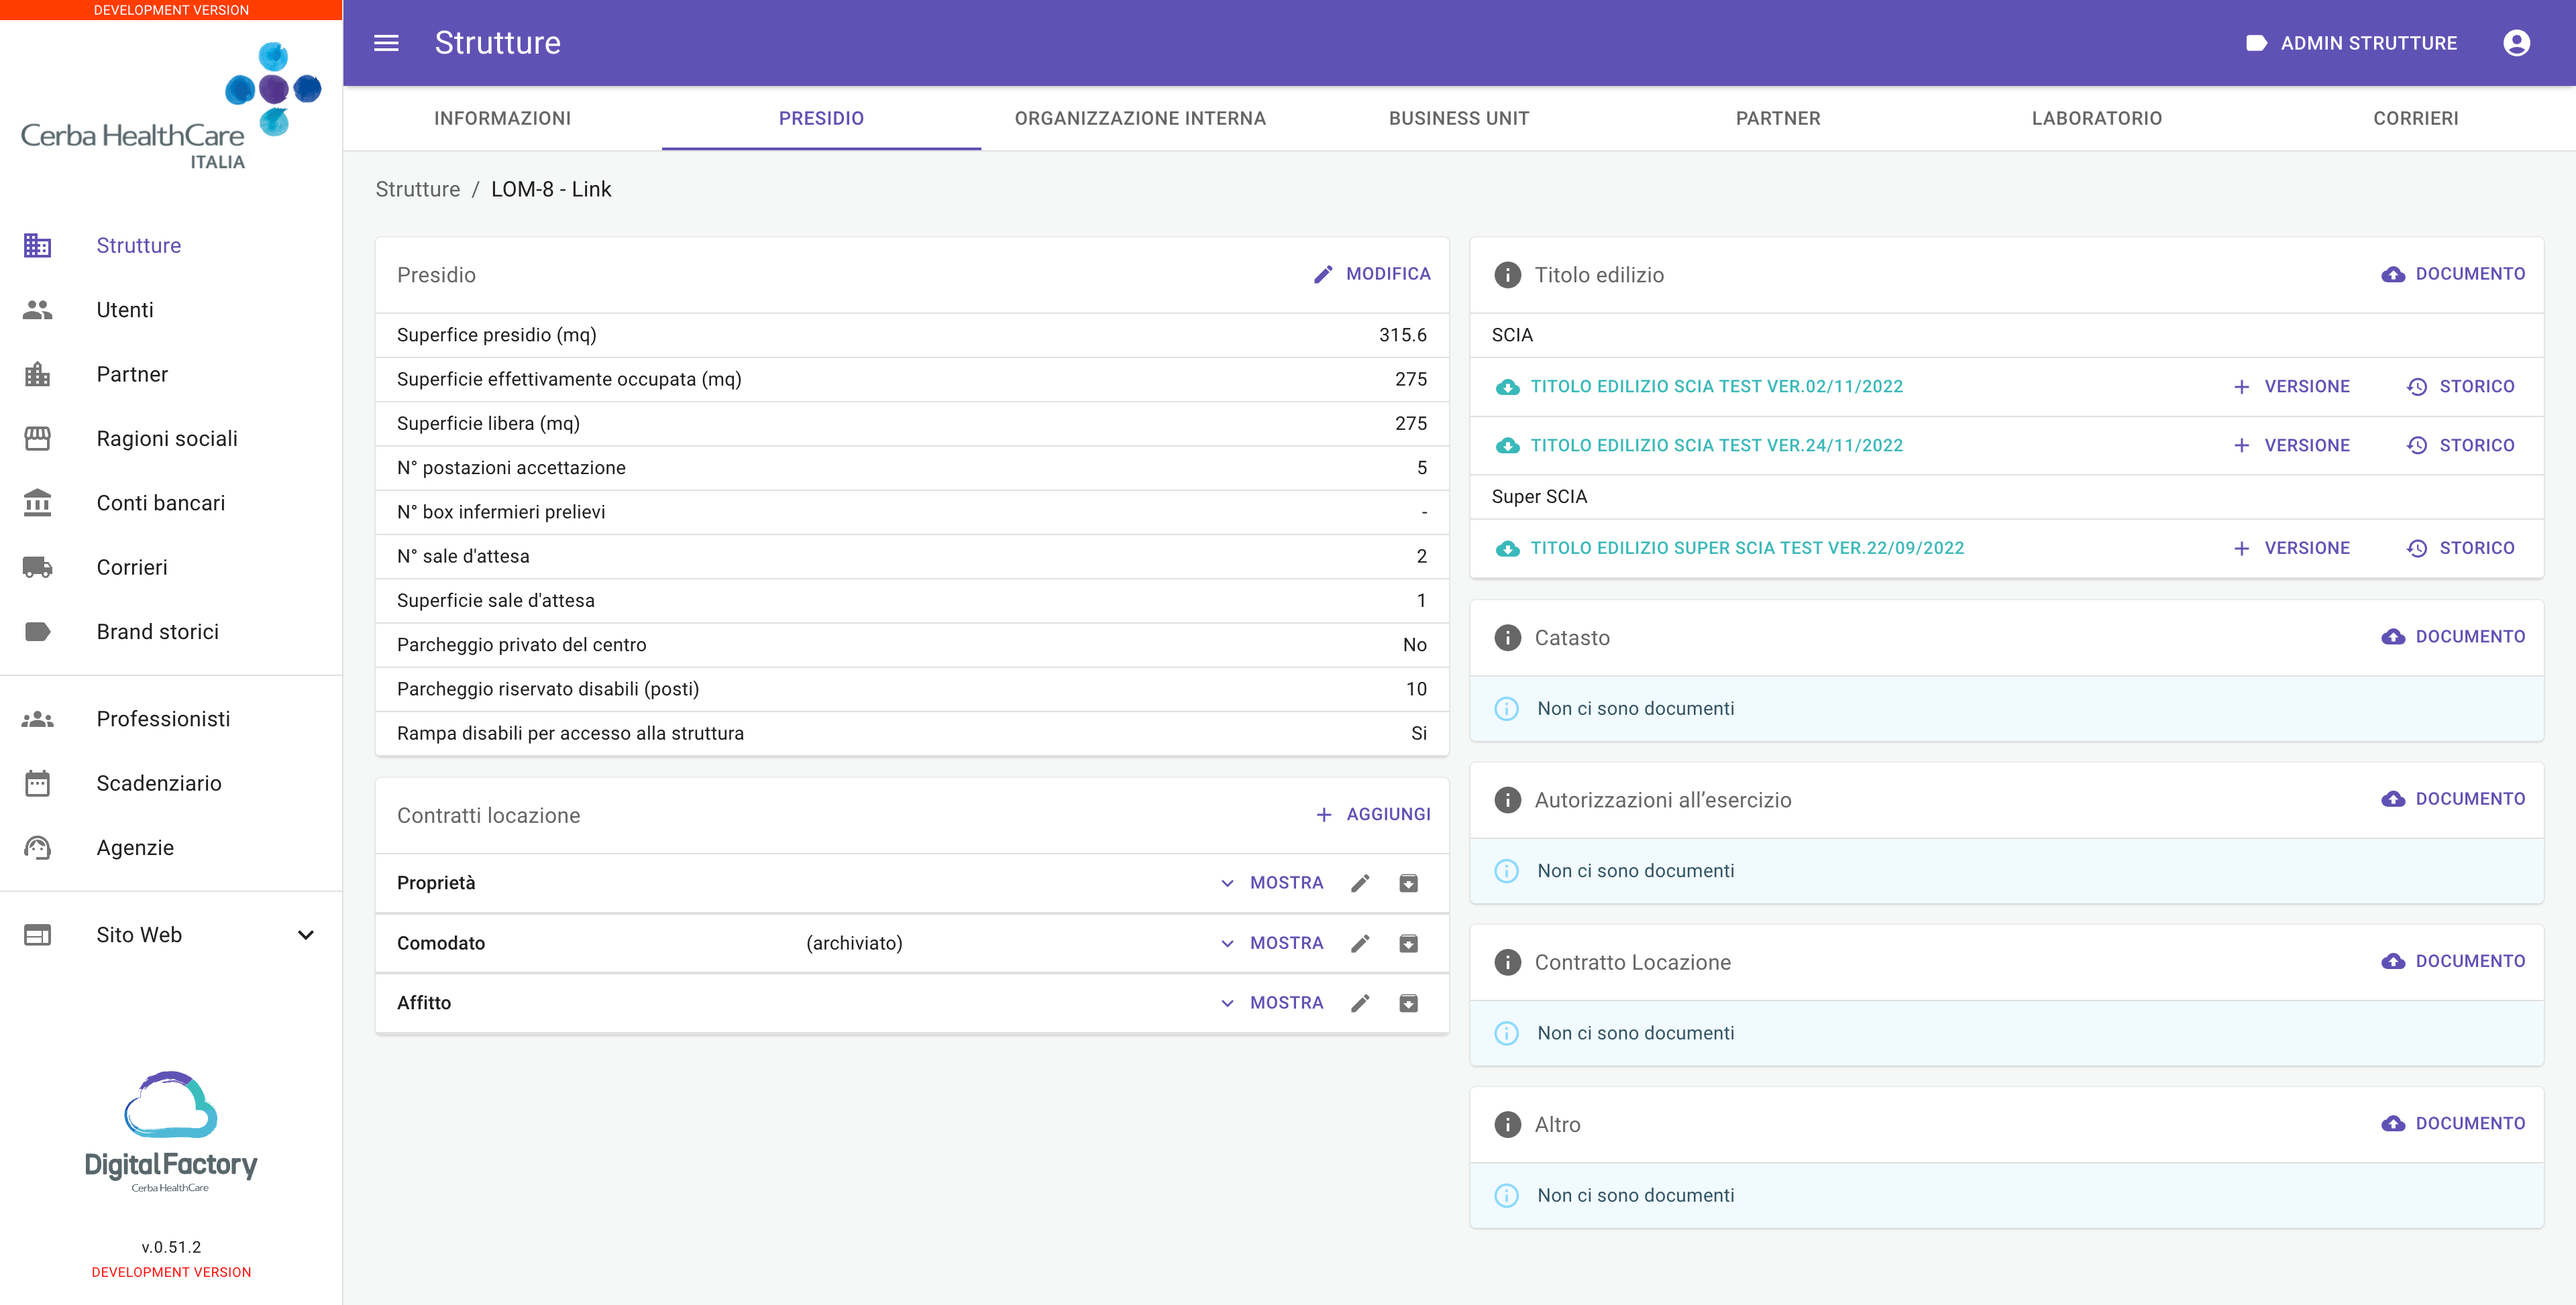
\includegraphics[width=0.75\textwidth]{images/capitolo5/f4_rentalAgreement/RentalAgreement_collapsed.png} 
    \caption{Tabella contratti non espansa} 
    \label{fig:RentalAgreement_collapsed}
\end{figure}

\begin{figure}[H]
    \centering
    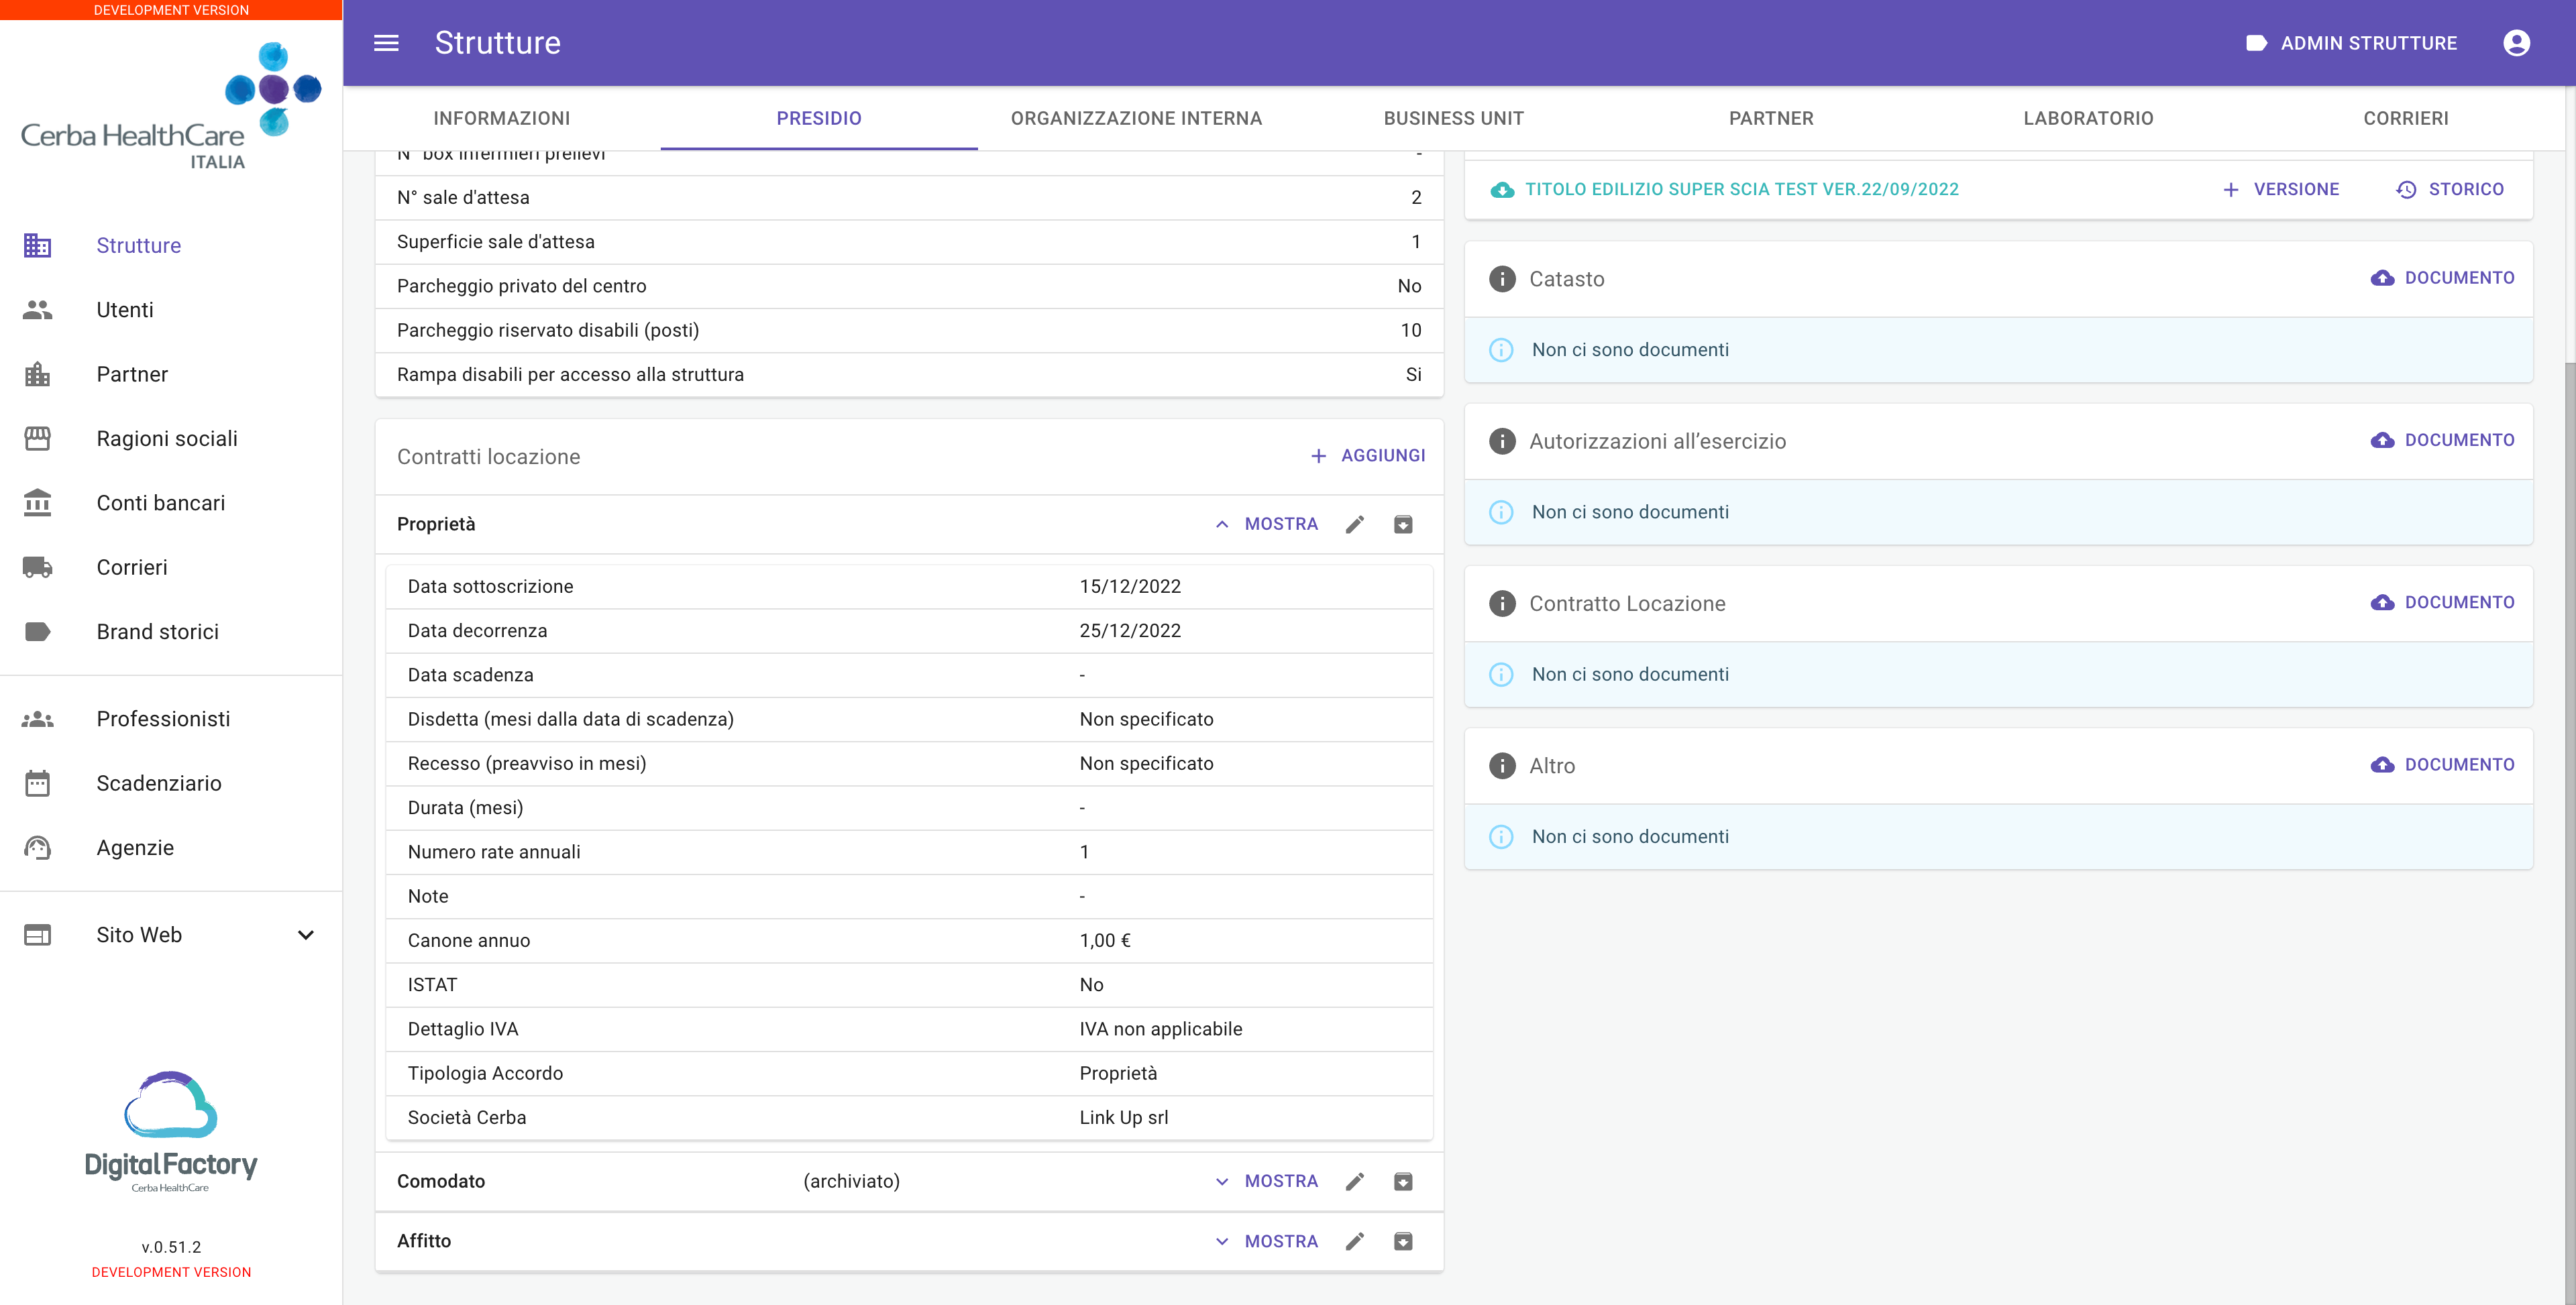
\includegraphics[width=0.75\textwidth]{images/capitolo5/f4_rentalAgreement/RentalAgreement_notCollapsed.png} 
    \caption{Tabella contratti con riga espansa} 
    \label{fig:RentalAgreement_notCollapsed}
\end{figure}

\newpage\section{F5: inserimento campo ricerca}
\label{sec:F5: inserimento campo ricerca}
La \textit{feature} F5 è stata caratterizzata da un certo livello di ridondanza: dopo la scrittura della nuova porzione di codice per la prima volta, l'implementazione è consistita semplicemente nella sua riproduzione dove previsto.\\
Nonostante piccole modifiche siano state operate di volta in volta ove necessario, i cambiamenti effettuati non rappresentano un qualcosa di così rilevante da giustificare  
l'inserimento dell'\textit{output} grafico di ogni situazione in cui l'implementazione è stata effettuata.

\subparagraph{Requisiti} 
L'\textit{header} della tabella di ognuna delle schede che formano la sezione “Ruoli Utente” (le schede sono: \textit{REO}, \textit{Area Manager}, \textit{Center Manager}, \textit{Data Manager}, \textit{Coordinatore Turni} e \textit{Coordinatore Compensi}) deve essere dotato di un campo di ricerca. Questo deve essere in grado di filtrare gli utenti per nome e/o cognome e posizionato alla sinistra del bottone per l'aggiunta di un ruolo utente.

\subparagraph{Procedura}
L'intero processo che ha portato all'implementazione del campo di ricerca all'interno della scheda del ruolo utente REO è avvenuto all'interno dello stesso componente, \texttt{TabReo}.

Il \textbf{primo \textit{step}} è consistito nella creazione della logica responsabile del suo funzionamento.\\
Ciò ha necessitato, \textit{in primis}, la dichiarazione della variabile di stato \texttt{filter} e del relativo \textit{setter} \texttt{setFilter()} attraverso l'\textit{hook} \texttt{useState()}. Tale variabile ha il compito di “memorizzare” il testo immesso, lato client, all'interno della casella di testo del campo di ricerca. Poiché, salvo introduzione di testo da parte dell'utente, il campo di ricerca si presenta come vuoto, la variabile \texttt{filter} è inizializzata con una stringa vuota \texttt{''}. Il contenuto di tale variabile viene aggiornato in continuazione con quanto scritto lato client attraverso il \textit{setter} \texttt{setFilter()}.

\lstinputlisting[caption=Variabile di stato \texttt{filter}, label=f5_TabReos_useState, language=JSX]{listings/capitolo5/f5_searchField/TabReos_useState.js}

In secondo luogo, è stata creata la variabile più propriamente responsabile del funzionamento della dinamica di ricerca, \texttt{filtered}. Questa implementa l'\textit{hook} \texttt{useMemo()} per il miglioramento delle \textit{performance} di esecuzione della ricerca.\\
All'interno del corpo di questa funzione è stata dichiarata la variabile \texttt{\_filter} (a riga 2): l'utilizzo dei metodi \texttt{toLowerCase()} e \texttt{trim()} sulla variabile di stato \texttt{filter}, assicura che il testo (in essa inserito ed immagazzionato) venga archiviato all'interno di un'altra variabile, \texttt{\_filter}, trasformato in minuscolo.\\
In seguito è stata dichiarata la variabile \texttt{filtered}: grazie allo \textit{spread operator} viene effettuata una copia di tutti i ruoli utente immagazzinati nella variabile \texttt{reos}\footnote{La variabile \texttt{reos}, assente nel \autoref{f5_TabReos_logic} perché già presente all'interno del codice, è frutto della chimata all'\gls{api} \texttt{getReos()}.}.\\
La condizione composta da un solo \texttt{if} ( da riga 6 a 12) costituisce la sezione più importante della variabile \texttt{filtered}; questa esprime il seguente concetto: se la lunghezza di \texttt{\_filter} è maggiore di \texttt{0}, sovrascrivi il precedente valore di \textit{filtered} con i soli utenti frutto del filtraggio, eseguito tramite l'iteratore \texttt{filter()}, sull'oggetto \texttt{filtered}.\\
Tale filtraggio, attraverso i metodi \texttt{toLowerCase()} e \texttt{includes()} sull'espressione che li precede, seleziona solo gli elementi (contenuti dalla variabile \texttt{filtered}) il cui nome e cognome o il cognome e nome in minuscolo include quando contenuto in \texttt{\_filter}.\\
In altre parole, vengono restituiti gli utenti del ruolo utente REO che corrispondono a quanto scritto all'interno del campo di ricerca.

\lstinputlisting[caption=Variabile \texttt{filtered}, label=f5_TabReos_UI, language=JSX]{listings/capitolo5/f5_searchField/TabReos_logic.js}

Il \textbf{secondo passaggio} è consistito nella creazione della porzione di interfaccia del campo di ricerca.\\
L' oggetto \texttt{table}\footnote{Il \textit{rendering} dell' oggetto \texttt{table} avviene grazie al componente \texttt{SuperTable} (all'interno del metodo \texttt{render()}). Per una speigazione più approfondita, si veda la \autoref{subsec:F6: “Magazine”}.} è stata modificata aggiungendo, all'interno della proprietà \texttt{action}, il componente \texttt{TextField}. Fra le molteplici \textit{props} di cui è dotato le più importanti sono:
\begin{itemize}
    \item \texttt{label}: il suo valore è la stringa \texttt{"Filtra per nome o cognome"};
    
    \item \texttt{placeholder}: il suo valore è la stringa \texttt{"Cerca"};
    
    \item \texttt{value}: il suo valore è la variabile di stato \texttt{filter};
    
    \item \texttt{onChange}: il suo valore è una funzione che permette di sostituire il contenuto della variabile di stato \texttt{filter} sfruttando il \textit{setter} \texttt{setFilter()}. Il nuovo contenuto sarà di volta in volta la proprietà \texttt{value} dell'oggetto \texttt{target} ( contenuto a sua volta dall'oggetto \texttt{e});
    
    \item \texttt{InputProps}: il suo valore è l'oggetto \texttt{endAdornment}, il quale contiene al suo interno i componenti \texttt{InputAdornment}, \texttt{IconButton} e \texttt{ClearButton}. Il componente \texttt{IconButton} è stato dotato della \textit{prop} \texttt{onClick} associata, di nuovo, al \textit{setter} \texttt{setFilter()}. In questo caso, però, il suo argomento è una stringa vuota \texttt{''} che serve per “azzerare” il valore della variabile \texttt{filter} ogni volta che viene effettuato click su quel bottone.
\end{itemize}

Infine, è stato modificato l'\textit{array} protagonista del \textit{mapping} utilizzato per popolare la proprietà \texttt{rows}, le righe, dell'oggetto \texttt{table}, della tabella.
La sostituzione del precedente con \texttt{filtered} fa in modo che, ogni qualvolta viene effettuata una ricerca scrivendo all'interno dell'apposito campo, vengano restituite, nella tabella dei REO, solamente le righe della  che corrispondono ai criteri specificati per il filtraggio.

\lstinputlisting[caption=Aggiornamento della variabile \texttt{table}, label=f5_TabReos_logic, language=JSX]{listings/capitolo5/f5_searchField/TabReos_UI.js}

\newpage\paragraph{\textit{Output} grafico}
\begin{figure}[H]
    \centering
    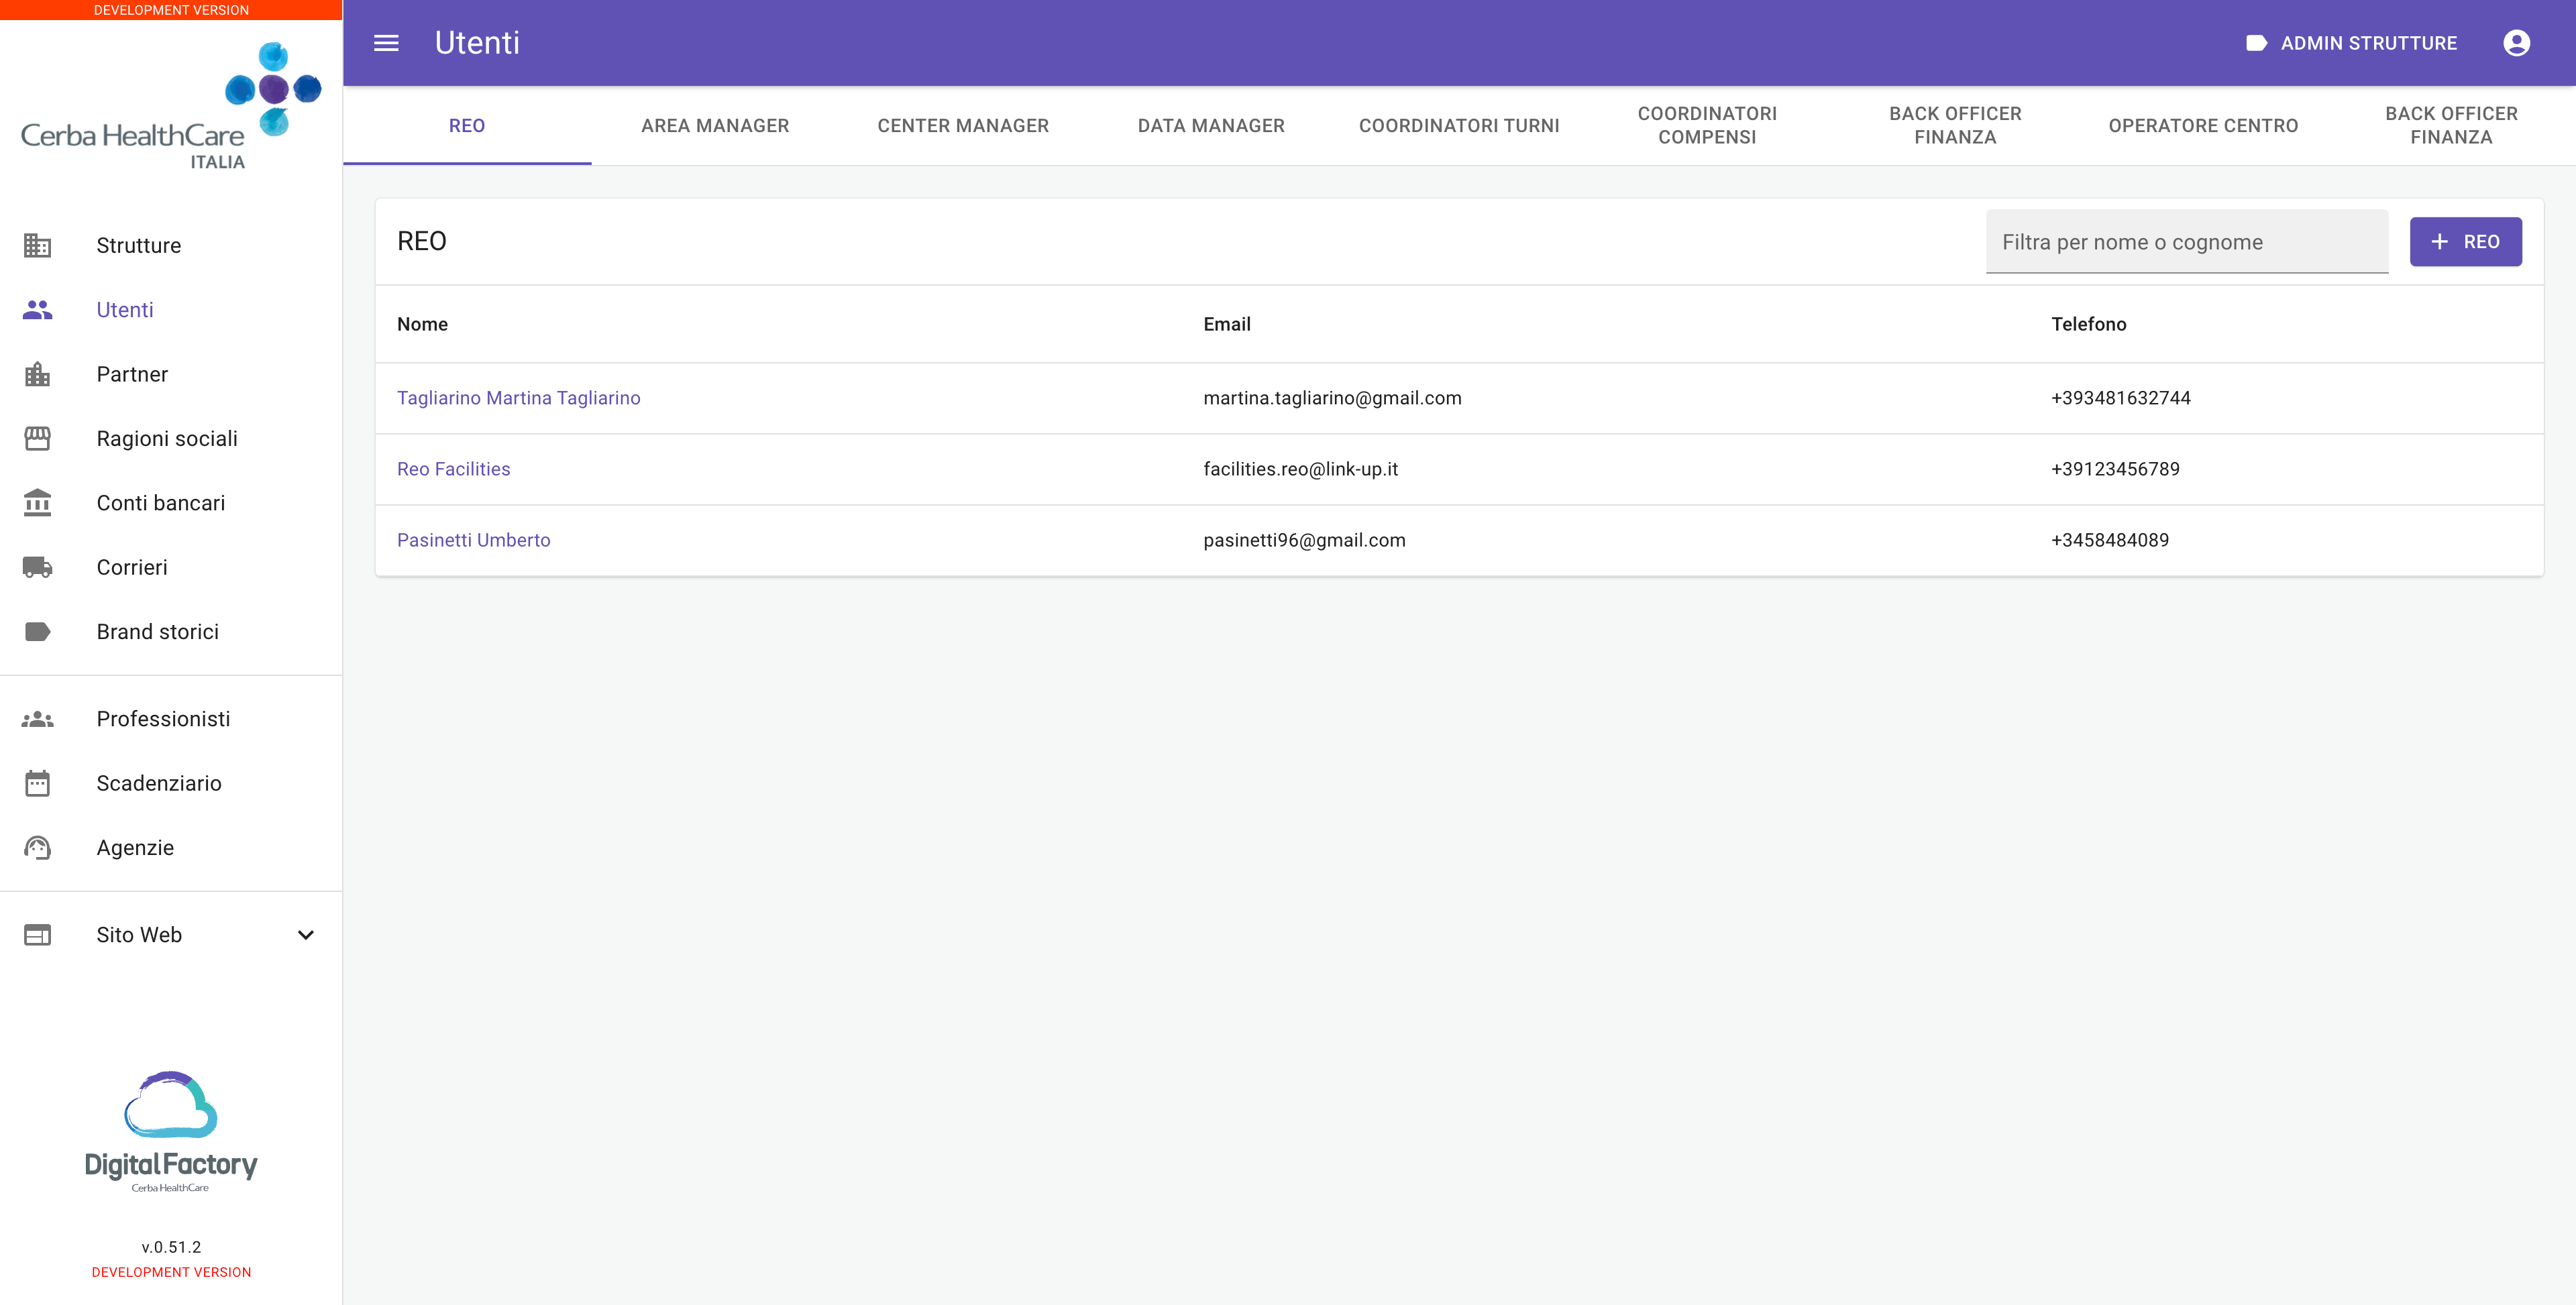
\includegraphics[width=0.75\textwidth]{images/capitolo5/f5_search/TabReo_searchEmpty.png} 
    \caption{Tabella REO campo ricerca vuoto} 
    \label{fig:TabReo_searchEmpty}
\end{figure}

\begin{figure}[H]
    \centering
    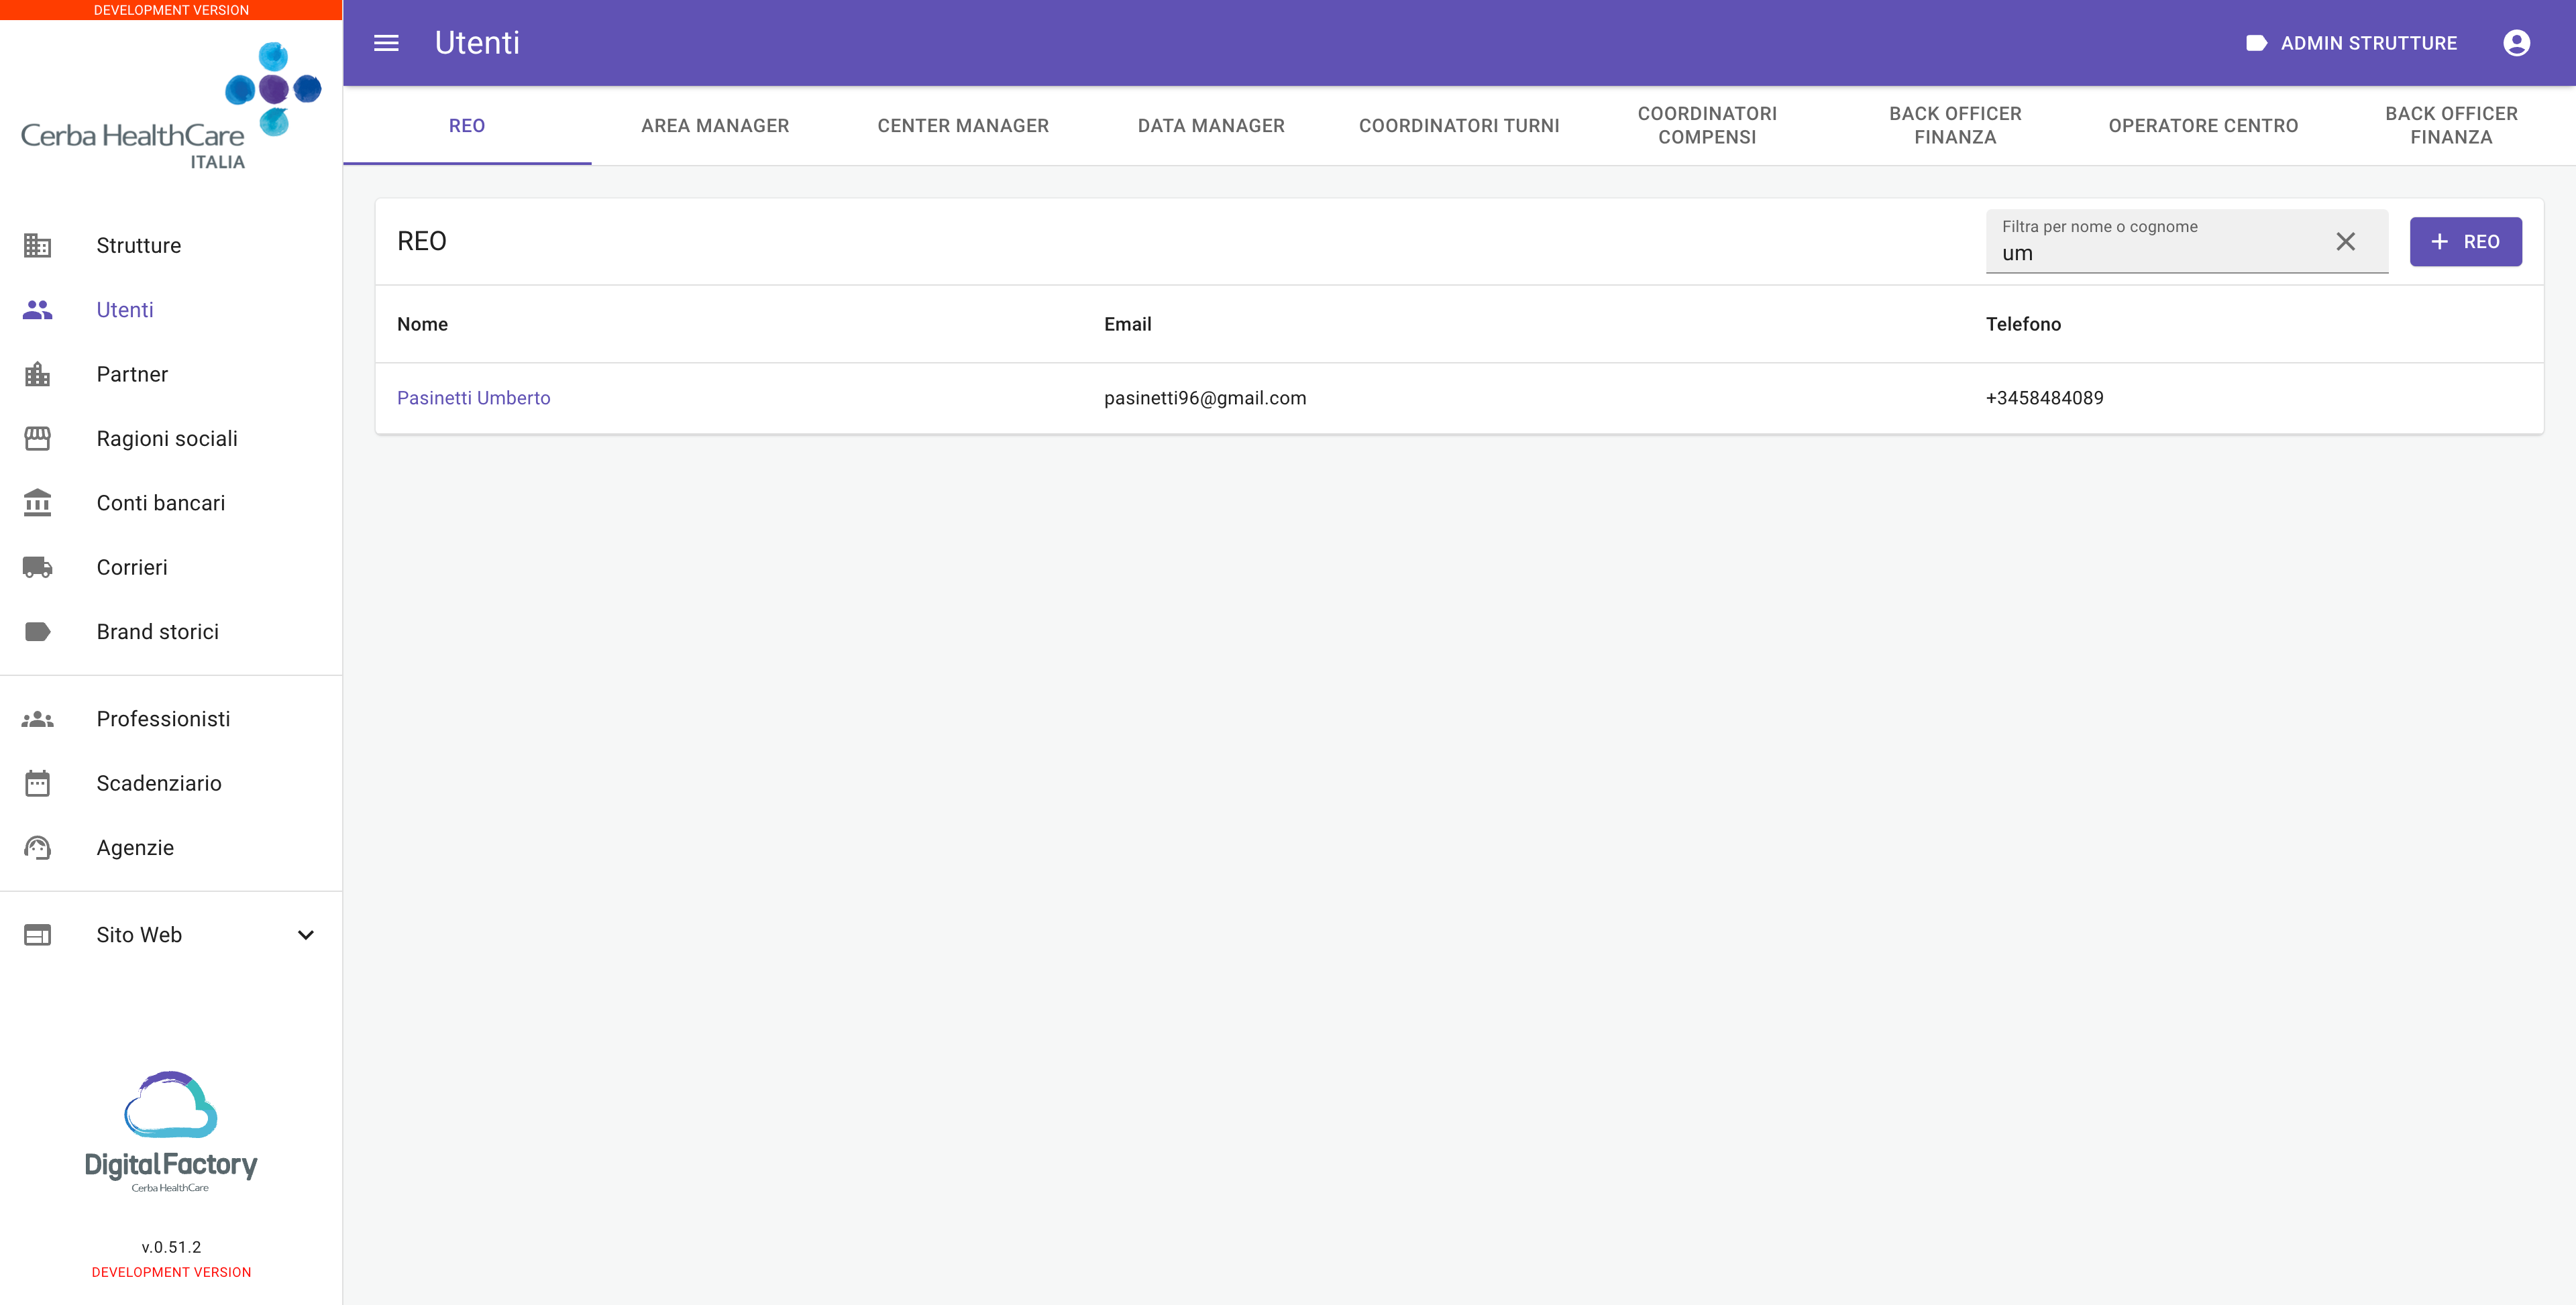
\includegraphics[width=0.75\textwidth]{images/capitolo5/f5_search/TabReo_searchFilled.png} 
    \caption{Tabella REO campo ricerca riempito} 
    \label{fig:TabReo_searchFilled}
\end{figure}

\newpage\section{F6 - F10: inserimento sezione}
Le \textit{feature} F6, F7, F8, F9 e F10 hanno previsto l'inserimento di una nuova sezione.\\
Da un lato, le sezioni di F6 e F7 sono state formate da una pagina per la visualizzazione dell'elenco degli elementi esistenti, e dalle modali per l'aggiunta, la modifica e l'eliminazione di un elemento. Nonostante dei cambiamenti siano stati effettuati ove necessario, le prime due \textit{feature} sono molto simili fra loro; per questo motivo si è optato di riportare solamente l'\textit{output} grafico relativo all'implementazione di F6.\\
Dall'altro, le sezioni di F8, F9 e F10 sono state composte da una pagina per la visualizzazione dell'elenco degli elementi, e da una pagina di dettaglio dedicata a ognuno di essi. A seconda dei casi, tramite le modali è possibile aggiungere, modificare o eliminare dati dell'elemento o l'elemento stesso. Anche qui le varie \textit{feature} non differiscono di molto, ma rispetto a quanto fatto per il precedente “gruppo” di implementazioni è stato riportato sia l'\textit{output} grafico di F8 che di F10.

\subsection{F6: “Magazine”}
\label{subsec:F6: “Magazine”}
\subparagraph{Requisiti}
Aggiungere la sezione “Magazine” fra quelle previste per il ruolo utente \textit{marketing admin}.\\
Al suo interno, una tabella deve mostrare i magazine esistenti in una lista semplice e riportarne le proprietà “Titolo”, “Descrizione”, “Data”, “Immagine” e “Documento”.\\
Deve essere possibile aggiungere o eliminare un magazine.\\
Deve essere possibile effettuare il download del documento.\\
Solamente per la proprietà “Descrizione” deve essere fornita la possibilità di formattazione.\\
L'\textit{header} della tabella dei magazine deve essere dotato di un campo di ricerca. Questo deve essere in grado di filtrare per titolo e posizionato alla sinistra del bottone per l'aggiunta di un nuovo magazine.

\subparagraph{Procedura}
Lo \textbf{\textit{step} iniziale} ha riguardato l'aggiornamento del \textit{routing}, operazione che ha comportato l'esecuzione di alcune modifiche all'interno del componente responsabile della navigazione fra le pagine visualizzate dal ruolo utente \textit{marketing admin}, ovvero \texttt{MarketingAdminRoutes}.\\
Come illustrato dal \autoref{f6_MarketingAdminRoutes}, il suo compito è sia il \textit{rendering} della \textit{dashboard}, ovvero del componente \texttt{DashboardMarketingAdmin}, che il contenimento dei vari componenti che definiscono il percorso che l'utente può seguire muovendosi nella piattaforma. La modifica al \textit{routing} ha necessitato l'inserimento, all'interno del componente padre \texttt{Switch} (da riga 3 a 9), di un nuovo componente figlio \texttt{Route}, il quale racchiude a sua volta \texttt{PageMagazines}, l'istanza del nuovo componente che verrà restituito cliccando sul link della sezione “Magazines”. L'istanza di \texttt{PageMagazines} è dotata della \textit{prop} \texttt{path}, il cui valore è la stringa \texttt{"/magazine"}.\\
In altre parole, la navigazione può ora avvenire, oltre che fra le vecchie pagine (o meglio, fra i vecchi componenti), anche su \texttt{PageMagazines}.

\lstinputlisting[caption=\textit{Routing} di \texttt{PageMagazines}, label=f6_MarketingAdminRoutes, language=JSX]{listings/capitolo5/f6_magazines/MarketingAdminRoutes.js}

Il \textbf{secondo passo} è consistito nell'aggiornamento della \textit{dashboard}, il “pannello” di controllo del ruolo utente \textit{marketing admin}; ciò ha richiesto dei ritocchi al componente \texttt{DashBoardMarketingAdmin}.\\ 
Per prima cosa, come possibile vedere nel \autoref{f6_DashboardMarketingAdmin_titles}, l'oggetto che contiene i titoli dell'\textit{header} della \textit{dashboard}, \texttt{titles}, è stato dotato della proprietà \texttt{'/magazine'}. La stringa \texttt{'Magazine'}, il suo valore, diverrà il titolo della sezione “Magazine”.

\lstinputlisting[caption=Aggiornamento variabile \texttt{titles}, label=f6_DashboardMarketingAdmin_titles, language=JSX]{listings/capitolo5/f6_magazines/DashboardMarketingAdmin_titles.js}
% spazio
In secondo luogo, come mostrato del \autoref{f6_DashboardMarketingAdmin_sidebar}, si è intervenuto sulla variabile che contiene la lista dei componenti che formano il menu laterale, \texttt{sidebar}, alla quale è stato aggiunto quello relativo alla sezione “Magazine”. Le \textit{props} del nuovo elemento \texttt{Sidebar} appena introdotto sono:
\begin{itemize}
    \item \texttt{label}: stabilisce il testo dell'etichetta della sezione nel menu laterale, il suo valore è la stringa \texttt{'Magazine'};
    
    \item \texttt{href}: stabilisce il percorso da seguire per visualizzare il componente, il suo valore è la stringa \texttt{'/magazine'};
    
    \item \texttt{icon}: stabilisce l'immagine da visualizzare accanto all'etichetta, il suo valore è il componente \texttt{NewspaperIcon}.
    
    % \item \texttt{isActive}: il suo valore è la funzione \texttt{isActive()};
\end{itemize}

\lstinputlisting[caption=Aggiornamento variabile \texttt{sidebar}, label=f6_DashboardMarketingAdmin_sidebar, language=JSX]{listings/capitolo5/f6_magazines/DashboardMarketingAdmin_sidebar.js}

Il \textbf{terzo passo} ha avuto a che fare con la creazione delle funzioni \texttt{getMagazines()}, \\\texttt{createMagazine()} e \texttt{deleteMagazine()}, le funzioni che effettuano le chiamate alle \gls{api} visibili nel \autoref{f6_api}. All'interno del loro corpo (alle righe righe 1, 4 e 7) sono state utilizzate, rispettivamente, le funzioni \texttt{get()}, \texttt{post()} e \texttt{del()}, funzioni che hanno il compito di effettuare le richieste avvalendosi dei metodi \texttt{GET}, \texttt{POST} e \texttt{DELETE}.

\lstinputlisting[caption=Funzioni di chiamata alle \gls{api} per la sezione “Magazine”, label=f6_api, language=JSX]{listings/capitolo5/f6_magazines/api.js}

Il \textbf{quarto} e \textbf{ultimo passo}, il più complesso e lungo, ha riguardato la modellazione dei componenti che formano la sezione “Magazine” e con i quali è possibile interagire.

% ! PageMagazine
\texttt{PageMagazines}, il primo realizzato (la cui istanza è stata vista nel \textit{routing} del ruolo utente \textit{marketing admin}), è illustrato nel \autoref{f6_PageMagazines_component} ed ha lo scopo di effettuare il \textit{rendering} della tabella che contiene la lista dei magazine.

\lstinputlisting[caption=Componente \texttt{PageMagazines}, label=f6_PageMagazines_component, language=JSX]{listings/capitolo5/f6_magazines/PageMagazines_component.js}
% spazio
Innanzitutto, al componente è stata fornita la logica necessaria per il suo funzionamento.\\
Come mostrato dal \autoref{f6_PageMagazines_get}, la funzione \texttt{getMagazines()} è passata come argomento all'\textit{hook} \texttt{useApi()} per reperire i magazine da visualizzare, \texttt{magazines}, le informazioni relative al caricamento e all'errore, \texttt{isLoading} ed \texttt{error}, e la funzione che permette di aggiornare la lista dei magazine, \texttt{fetchMagazines}.

\lstinputlisting[caption=Utilizzo \texttt{getMagazines()}, label=f6_PageMagazines_get, language=JSX]{listings/capitolo5/f6_magazines/PageMagazines_get.js}
% spazio
I due \textit{handler} dichiarati in \texttt{PageMagazines} sono \texttt{handleDeleteMagazine()} e \\\texttt{handleConfirmDeleteMagazine}. Come mostrato nel \autoref{f6_PageMagazines_handlers}, se da un lato, il primo è noto per struttura e scopo poiché già incontrato nella \autoref{sec:F4: modifica tabella contratti di locazione}, dall'altro, il secondo costituisce un qualcosa di completamente nuovo.\\
La funzione \texttt{handleDeleteMagazine}, infatti, appartiene a quel gruppo di \textit{handler} che hanno il compito di aprire una modale, e le operazioni che esegue sono: 
\begin{enumerate}
    \item L'impostazione, tramite il \textit{setter} \texttt{setData()}, dei dati della modale \\\texttt{modalConfirmDeleteMagazine}, sull'oggetto \texttt{magazine};
    
    \item L'apertura della modale tramite la funzione \texttt{open()}.
\end{enumerate}
Gli oggetti relativi alla modale \texttt{modalConfirmDeleteMagazine} e \texttt{modalMagazine} sono stati dichiarati attraverso il \textit{custom hook} \texttt{useModal()} (alle righe riga 1 e 3); \texttt{modalMagazine} è utilizzata per l'aggiunta di nuovi magazine.\\
L'\textit{handler} \texttt{handleConfirmDeleteMagazine}, invece, è una funzione atta all'effettiva manipolazione dei dati, e le operazioni che esegue sono: 
\begin{enumerate}
    \item L'eliminazione, dal \textit{bucket} \texttt{marketing}, della proprietà \texttt{path} dell'oggetto \texttt{0} all'interno dell'\textit{array} \texttt{files} (contenuto a sua volta, a risalire, dagli oggetti \texttt{document}, \texttt{magazine}, \texttt{data} e \texttt{modalConfirmDeleteMagazine}), con l'invocazione della funzione \texttt{removeToS3()};
    
    \item L'eliminazione, dal \textit{bucket} \texttt{marketing}, della proprietà \texttt{path} contenuta dall'oggetto \texttt{image} (contenuta a sua volta, a risalire, da \texttt{magazine}, \texttt{data} e \texttt{modalConfirmDeleteMagazine}), con l'invocazione della funzione \texttt{removeToS3()};
    
    \item L'effettiva eliminazione del magazine, con l'invocazione della funzione \texttt{deleteMagazine()}, alla quale viene passato come argomento l'\texttt{uuid} dell'oggetto \texttt{magazine} (contenuto a sua volta, a risalire, dagli oggetti \texttt{data} e \texttt{modalConfirmDeleteMagazine});
    
    \item L'aggiornamento della lista dei magazine, con l'invocazione della funzione \texttt{fetchMagazines()}.
\end{enumerate}

\lstinputlisting[caption=\textit{Handler} componente \texttt{PageMagazines}, label=f6_PageMagazines_handlers, language=JSX]{listings/capitolo5/f6_magazines/PageMagazines_handlers.js}
% spazio
\texttt{PageMagazines} contiene poi la logica relativa al campo di ricerca. Il suo funzionamento è sostanzialmente identico a quello visto nella \autoref{sec:F5: inserimento campo ricerca}, ma la sua struttura si differenzia parzialmente da quella della \textit{feature} F5.\\
La dinamica di filtraggio è qui inserita all'interno dell'\textit{hook} \texttt{useEffect()}; inoltre, la condizione \texttt{if} (a riga 9) si caratterizza per il fatto che il valore/i restituito dal filtraggio\footnote{Il valore restituito dal filtraggio è assegnato alla variabile \texttt{\_filtered}.}, effettuato nuovamente tramite l'iteratore \texttt{filter()}, corrisponde all'elemento/i, all'interno dei magazine, il cui titolo in minuscolo corrisponde a quando presente nella variabile \texttt{\_filterName}. 

\lstinputlisting[caption=Dinamica di filtraggio della sezione magazine, label=f6_PageMagazines_search, language=JSX]{listings/capitolo5/f6_magazines/PageMagazines_search.js}
% spazio
La logica del primo componente creato si è conclusa specificando la posizione del \textit{bucket} in cui sono contenute le immagini associate ai magazine. Ciò è stato fatto grazie alla funzione \texttt{configure()} (invocata sull'oggetto \texttt{Amplify}), alla quale è passato come argomento un oggetto la cui unica proprietà, \texttt{Storage}, ha per valore l'ubicazione, ovvero la proprietà \texttt{marketing} di \texttt{storage} (contenuta, a risalire, dagli oggetti \texttt{amplify} e \texttt{config}). 

\lstinputlisting[caption=Configurazione di \texttt{Amplify}, label=f6_PageMagazines_amplifyConfigure, language=JSX]{listings/capitolo5/f6_magazines/PageMagazines_amplifyConfigure.js}
% spazio
Dopodiché, è stata modellata la \acrshort{ui} di \texttt{PageMagazines}. Il \textit{rendering} di questo componente avviene in modo particolare: all'interno della sua logica, è dichiarato un oggetto, \texttt{table}, che specifica tutte le caratteristiche della tabella da visualizzare, e che viene passato, sotto forma di \textit{prop}, a un componente, \texttt{SuperTable}, che “impagina” \texttt{table} ritornando a schermo la tabella dei magazine.\\
Per questo motivo, la gestione della veste grafica di \texttt{PageMagazines} è consistita principalmente nella manipolazione dell'oggetto \texttt{table}\footnote{L'oggetto \texttt{table} deve essere costruito necessariamente includendo proprietà che possono essere accettate dal componente \texttt{SuperTable}.}, le cui proprietà sono:
\begin{itemize}
    \item \texttt{title} (a riga 2): specifica il titolo della tabella, il suo valore è la stringa \texttt{'Magazine'};
    
    \item \texttt{noResults} (a riga 2): specifica il messaggio da restituire se la tabella è vuota, il suo valore è la stringa \texttt{'Nessun magazine trovato'};
    
    \item \texttt{action} (da riga 3 a 31): specifica le azioni che possono essere compiute nell'\textit{header} della tabella, il suo valore è un'espressione che permette di effettuare:
        \begin{itemize}
            \item La ricerca di un magazine fra quelli esistenti grazie al componente \texttt{TextField} (da riga 5 a 22). Le molteplici \textit{props} di cui è dotato sono sostanzialmente identiche a quelle descritte in relazione al medesimo componente nella \textit{feature} F5\footnote{Si veda la \autoref{sec:F5: inserimento campo ricerca}.};
            
            \item L'aggiunta di un nuovo magazine grazie al componente \texttt{Button} (da riga 24 a 29). Il testo restituito dal componente è “Magazine” e le sue più importanti \textit{props} sono:
            \begin{itemize}
                \item \texttt{onClick} (a riga 25): il suo valore è la funzione \texttt{open()} invocata sull'oggetto \texttt{modalMagazine};
                
                \item \texttt{startIcon} (a riga 26): il suo valore è il componente \texttt{AddIcon};
            \end{itemize}
        \end{itemize}
    
    \item \texttt{isLoading} e \texttt{error} (a riga 32): specificano delle informazioni relative allo stato di una chiamata ad un'\gls{api};
     
    \item \texttt{filter} (a riga 32): specifica il messaggio da ritornare sotto l'\textit{header} della tabella una volta eseguita una ricerca;
    
    \item \texttt{perPage} (a riga 32): specifica il numero di elementi da visualizzare in una pagina, il suo valore è \texttt{10};
    
    \item \texttt{headers} (da riga 33 a 40): specifica i titoli delle colonna della tabella, il suo valore è un'oggetto che, a sua volta, include gli oggetti \texttt{title}, \texttt{description}, \texttt{date}, \texttt{image}, \texttt{document} e \texttt{delete}. All'interno di ognuno di essi sono definite le caratteristiche del titolo stesso attraverso le proprietà:
        \begin{itemize}
            \item \texttt{label}: stabilisce il testo del titolo di una colonna, il suo valore è una stringa, ad esempio, \texttt{'Titolo'};
            
            \item \texttt{sort}: stabilisce se è possibile effettuare l'ordinamento dei magazine in base alla proprietà della colonna in considerazione, il suo valore è un valore booleano, ad esempio, \texttt{true};
            
            \item \texttt{width}: stabilisce la larghezza della colonna, il suo valore è un numero, ad esempio, \texttt{40};  
        \end{itemize}   
    \item \texttt{rows} (da riga 41 a 57): specifica il contenuto delle righe della tabella, il suo valore è il \textit{mapping} dell'\textit{array} \texttt{filtered}. Da un lato, l'\textit{array} \texttt{filtered} permette di visualizzare, ogni qualvolta viene effettuata una ricerca, solamente le righe della tabella che corrispondono a quanto cercato; dall'altro, se non viene effettuata nessuna ricerca, consente semplicemente di effettuare il \textit{rendering} della lista dei magazine.\\
    Tramite il \textit{mapping}, le proprietà di cui ogni elemento dell'\textit{array} è fornito sono:
    \begin{itemize}
        \item \texttt{key} (a riga 42): il suo valore è la proprietà \texttt{uuid} dell'oggetto \texttt{el};
        
        \item \texttt{title} (a riga 42): specifica il titolo, il suo valore è la proprietà \texttt{title} dell'oggetto \texttt{el};
        
        \item \texttt{description} (a riga 43): specifica la descrizione, il suo valore è il componente \texttt{Box}. Questo permette di visualizzare la descrizione, originariamente in formato HTML, come normale testo, mantenendo la formattazione fornitagli lato client. Ciò avviene grazie alla \textit{prop} \texttt{dangerouslySetInnerHTML} passata al componente \texttt{Box}: il suo valore è un oggetto la cui unica proprietà, \texttt{\_\_html}, ha come valore la descrizione del magazine, ovvero la proprietà \texttt{description} dell'oggetto \texttt{el};
        
        \item \texttt{date} (a riga 44): specifica la data, il suo valore è la proprietà \texttt{date}  dell'oggetto \texttt{el}, la quale viene formattata con il metodo\texttt{format()}\footnote{Si veda la \autoref{subsec:date-fns}};
        
        \item \texttt{image} (a riga 45): specifica l'immagine, il suo valore è l'istanza del componente \texttt{Image}. L'unica \textit{prop} che le viene passata è \texttt{el}, il cui valore è quello del singolo oggetto che sta venendo mappato, \texttt{el};
        
        \item \texttt{document} (a riga 46): specifica il documento, il suo valore è il componente \texttt{DownloadDocument}. Le \textit{props} passategli sono:
        \begin{itemize}
            \item \texttt{action}: stabilisce il testo visualizzato dal componente. Il suo valore è la proprietà \texttt{name} (contenuta, a risalire, dagli oggetti \texttt{document} e \texttt{el});
            
            \item \texttt{storage}: stabilisce la posizione del documento per effettuarne il download, il suo valore è la stringa \texttt{'Marketing'};
            
            \item \texttt{path}: stabilisce il percorso per reprire il documento per effettuarne il download, il suo valore è la proprietà \texttt{path} contenuta nell'oggetto \texttt{0} dell'\textit{array} \texttt{files} (contenuto, a sua volta, dagli oggetti \texttt{document} ed \texttt{el}).
        \end{itemize}
        
        \item \texttt{delete} (a riga 52): specifica il bottone per l'eliminazione di un magazine, il suo valore è il componente \texttt{IconButton}. L'unica \textit{prop} fornitagli è \texttt{onClick}, il cui valore è l'\textit{handler} \texttt{handleDeleteMagazine()} a cui viene passato come argomento \texttt{el}, l'oggetto del magazine che si vuole eliminare. All'interno di \texttt{IconButton} è presente il componente \texttt{DeleteIcon}.
    \end{itemize} 
\end{itemize}

\lstinputlisting[caption=Oggetto \texttt{table}, label=f6_PageMagazines_UI_table, language=JSX]{listings/capitolo5/f6_magazines/PageMagazines_UI_table.js}
% spazio
Il \autoref{f6_PageMagazines_UI_return} mostra come il \textit{rendering} della tabella avvenga tramite il componente \texttt{SuperTable} (a riga 2), al quale viene passata come unica \textit{prop} \texttt{table}, il cui valore è l'oggetto \texttt{table} appena discusso.\\
Al suo interno, è mostrato anche come le modali per l'aggiunta e l'eliminazione di un magazine vengano restituite condizionalmente attraverso l'operatore logico AND.\\
Nel primo caso, se la proprietà \texttt{isOpen} dell'oggetto \texttt{modalMagazine} è vera, allora viene restituito il componente \texttt{ModalMagazine}; le \textit{props} passategli sono:
\begin{itemize}
    \item \texttt{modal}: stabilisce la modale in uso, il suo valore è l'oggetto \texttt{modalMagazine};
    
    \item \texttt{magazine}: stabilisce le proprietà del magazine, il suo valore è un oggetto vuoto (\texttt{\{\}});
    
    \item \texttt{onSaved}: stabilisce la funzione da invocare per l'aggiornamento della lista dei magazine, il suo valore è la funzione \texttt{fetchMagazines()}.
\end{itemize}
% spazio
Allo stesso modo, nel secondo caso, se la proprietà \texttt{isOpen} dell'oggetto \\\texttt{modalConfirmDeleteMagazine} è vera, allora viene restituito il componente \texttt{ModalConfirm}; le \textit{props} passategli sono:
\begin{itemize}
    \item \texttt{modal}: il suo valore è l'oggetto \texttt{modalConfirmDeleteMagazine};
    
    \item \texttt{title}: stabilisce il titolo della modale di conferma eliminazione, il suo valore è la stringa \texttt{"Eliminazione magazine"};
    
    \item \texttt{text}: stabilisce il testo del messaggio mostrato dalla modale di conferma eliminazione, il suo valore è la stringa \texttt{"Eliminare il magazine?"};
    
    \item \texttt{handleConfirm}: stabilisce la funzione da invocare per l'effettiva eliminazione del magazine.
\end{itemize}

\lstinputlisting[caption=\texttt{SuperTable} e modali, label=f6_PageMagazines_UI_return, language=JSX]{listings/capitolo5/f6_magazines/PageMagazines_UI_return.js}

% ! Image
\texttt{Image}, il secondo componente creato (la cui istanza è stata vista nella \acrshort{ui} di \texttt{PageMagazines}), ha il solo compito di reperire l'immagine di un magazine.\\
Come mostrato dal \autoref{f6_Image_component}, la sua dichiarazione è stata accompagnata dall'importazione della \textit{prop} \texttt{el}, l'unica che gli viene passata durante il \textit{mapping} effettuato nella proprietà \texttt{rows} dell'oggetto \texttt{table}.

\lstinputlisting[caption=Componente \texttt{Image}, label=f6_Image_component, language=JSX]{listings/capitolo5/f6_magazines/Image_component.js}
% spazio
La logica di \texttt{Image} è molto semplice. Da un lato, come possibile vedere nel \autoref{f6_Image_useState}, sono stati dichiarati la varibile di stato \texttt{image}, che ha il compito di “memorizzare” l'immagine da reperire, ed il relativo \textit{setter} \texttt{setImage()}; la variabile di stato è stata inizializzata con il valore \texttt{null}.

\lstinputlisting[caption=Variabile di stato \texttt{image} di \texttt{Image}, label=f6_Image_useState, language=JSX]{listings/capitolo5/f6_magazines/Image_useState.js}
% spazio
Dall'altro, come illustrato dal \autoref{f6_Image_useEffect}, l'\textit{hook} \texttt{useEffect()} consente di reperire l'immagine. All'interno del suo corpo, ciò avviene grazie a una condizione che utilizza un singolo \texttt{if} (da riga 2 a 6) per esprimere il seguente concetto: se l'oggetto \texttt{el} è vero, allora recupera la proprietà \texttt{path} dell'oggetto \texttt{image}(contenuta, a risalire, dall' oggetto \texttt{el}), tramite la funzione \texttt{get()} (invocata sull'oggetto \texttt{Storage}); in seguito, sostituisci il precedente valore della variabile di stato \texttt{image} con \texttt{url}, grazie al \textit{setter} \texttt{setImage()}, 

\lstinputlisting[caption=\texttt{useEffect()} di \texttt{Image}, label=f6_Image_useEffect, language=JSX]{listings/capitolo5/f6_magazines/Image_useEffect.js}
% spazio
Invece, la \acrshort{ui} di \texttt{Image} è costituita solamente dal componente \texttt{CardMedia}, le cui più importanti \textit{props} sono:
\begin{itemize}
    \item \texttt{image}: il suo valore è \texttt{image};
    
    \item \texttt{alt}: stabilisce qual è il testo alternativo, il suo valore è la proprietà \texttt{image} dell'oggetto \texttt{el}.
\end{itemize}

\lstinputlisting[caption=UI \texttt{Image}, label=f6_Image_UI, language=JSX]{listings/capitolo5/f6_magazines/Image_UI.js}

% ! ModalMagazine
% ! manca qualche cagatina sul finale
Infine, \texttt{ModalMagazine} (la cui istanza è stata vista nel \textit{renering} condizionale delle modali, a seguito di \texttt{SuperTable}) è il terzo e ultimo componente creato per la sezione “Magazine”; il suo compito è la creazione di un nuovo magazine. Come mostrato dal \autoref{f6_ModalMagazine_component}, la sua dichiarazione è stata accompagnata dall'importazione delle \textit{prop} \texttt{modal} e \texttt{onSaved}.

\lstinputlisting[caption=Componente \texttt{ModalMagazine}, label=f6_ModalMagazine_component, language=JSX]{listings/capitolo5/f6_magazines/ModalMagazine_component.js}
% spazio
Anche in questo caso, per prima cosa è stata definita la logica del componente. Come mostrato dal \autoref{f6_ModalMagazine_useState}, all'interno del componente \texttt{ModalMagazine}, per ogni proprietà posseduta da un magazine è stata dichiarata una variabile di stato e il relativo \textit{setter} tramite l'\textit{hook} \texttt{useState()}. Il compito di queste variabili è la “memorizzazione” dei valori immessi, lato client, durante l'aggiunta di un nuovo magazine. Il valore con cui sono state inizializzate differisce a seconda del tipo di dato attesso: \texttt{title}, \texttt{description}, \texttt{image\_alt} e \texttt{doc\_name} hanno come valore di inizio una stringa vuota (\texttt{''}), mentre \texttt{date}, \texttt{image} e \texttt{doc} hanno \texttt{null}.

\lstinputlisting[caption=Variabili di stato di \texttt{ModalMagazine}, label=f6_ModalMagazine_useState, language=JSX]{listings/capitolo5/f6_magazines/ModalMagazine_useState.js}
% spazio
In seguito, come mostrato dal \autoref{f6_ModalMagazine_schema}, è stato definito l'oggetto \texttt{schema}. Al suo interno, le proprietà, anche in questo caso, riflettono quelle possedute dal magazine da aggiungere e il loro valore riflette i vincoli che devono essere rispettati dall'utente al momento di immissione dei dati.

\lstinputlisting[caption=Oggetto \texttt{shema} di \texttt{ModalMagazine}, label=f6_ModalMagazine_schema, language=JSX]{listings/capitolo5/f6_magazines/ModalMagazine_schema.js}
% spazio
Come illustrato dal \autoref{f6_ModalMagazine_cHooks}, inoltre, dentro a \texttt{ModalMagazine} sono stati effettuati:
\begin{itemize}
    \item Il “recupero” delle funzioni \texttt{validate()}, \texttt{validateField()}, \texttt{validation()} e \\\texttt{validationProps()} con l'\textit{hook} \texttt{useValidation()} (a riga 1 e 2);
    
    \item La dichiarazione dell'oggetto \texttt{status} con l'\textit{hook} \texttt{useStatus()} (a riga 4);
    
    \item La dichiarazione dell'oggetto \texttt{descriptionRef} con l'\textit{hook} \texttt{useRef()} (a riga 5);
\end{itemize}

\lstinputlisting[caption=\textit{Custom hooks} di \texttt{ModalMagazine}, label=f6_ModalMagazine_cHooks, language=JSX]{listings/capitolo5/f6_magazines/ModalMagazine_cHooks.js}
% spazio
La parte più importante della logica di \texttt{ModalMagazine} è quella riguardante l'\textit{handler} \texttt{onClick}, funzione che (come \texttt{handleConfirmDeleteMagazine}) si occupa dell'effettiva manipolazione di dati. Come possibile vedere nel \autoref{f6_ModalMagazine_onClick}, le operazioni che esegue sono:
\begin{enumerate}
    \item La dichiarazione dell'oggetto \texttt{form}, le cui proprietà sono le variabli di stato definite in precedenza (da riga 2 a 4);
    
    \item La valutazione di una condizione \texttt{if} (da riga 6 a 38) che stabilisce che, se la validazione dell'oggetto \texttt{form}, tramite l'invocazione della funzione \texttt{validate()}, è avvenuta correttamente, può essere eseguita un'altra serie di operazioni. Da un lato, fra di esse vi è il tentativo, \texttt{try} (da riga 7 a 35), di eseguire le seguenti istruzioni:
        \begin{enumerate}
            \item L'impostazione dello stato su “caricamento” con l'invocazione del metodo \\\texttt{setLoading()} (sull'oggetto \texttt{status}, a riga 8);
    
            \item La dichiarazione della variabile \texttt{import\_image}, che carica l'immagine, \texttt{image}, e il suo testo alternativo, \texttt{image\_alt}, all'interno del \textit{bucket} \texttt{marketing} (da riga 10 a 12);
    
            \item La dichiarazione della variabile \texttt{import\_doc}, che carica il documento, \texttt{doc}, e il suo nome, \texttt{doc\_name}, all'interno del \textit{bucket} \texttt{marketing} (da riga 14 a 16);
    
            \item La dichiarazione dell'oggetto \texttt{body}, le cui proprietà sono le variabili di stato definite precedentemente a eccezione di \texttt{description}, \texttt{image} e \texttt{document}. I valori a esse fornite sono, rispettivamente, il valore ritornato dalla conversione del contenuto della variabile di stato \texttt{description}, con l'invocazione della funzione \texttt{htmlFromRaw()}; tutte le proprietà dell'oggetto \texttt{file} (contenuto dall'oggetto \texttt{import\_image}) uguali tranne \texttt{alt}, a cui viene assegnato il contenuto della variabile di stato \texttt{image\_alt}; la proprietà \texttt{date} e le proprietà \texttt{name} e \texttt{file} a cui sono assegnati, rispettivamente, i valori delle variabili di stato \texttt{doc\_name} e l'oggetto \texttt{file} (contenuto dall'oggetto \texttt{import\_doc}) (da riga 18 a 26);
    
            \item L'effettiva creazione del nuovo magazine con l'invocazione della funzione di chiamata all'\gls{api} \texttt{createMagazione()}; i dati del nuovo magazine saranno quelli contenuti nell'oggetto \texttt{body} creato poco fa, il quale viene passato come argomento alla funzione \texttt{createMagazine()} (a riga 28).
            
            \item L'impostazione dello stato su “successo” con l'invocazione della funzione \texttt{setSuccess()} (sull'oggetto \texttt{status}) (a riga 30); 
            
            \item L'aggiornamento della lista dei magazine con l'invocazione della funzione \texttt{onSaved()}. Il suo valore è la funzione \texttt{fetchMagazines}, la quale era stata passata al componente \texttt{modalMagazine} come valore della \textit{prop} \texttt{onSaved} (a riga 32);
            
            \item La chiusura della modale con l'invocazione della funzione \texttt{close()} (sull'oggetto \texttt{modal}) (a riga 34).
        \end{enumerate}
    Dall'altro lato, fra le operazioni previste dalla condizione \texttt{if}, vi è il recupero, \texttt{catch}, dell'errore, \texttt{err}, e la conseguente impostazione dello stato su “errore” con l'invocazione della funzione \texttt{setError()} (sull'oggetto \texttt{status}) (da riga 35 a 37).
\end{enumerate}

\lstinputlisting[caption=\textit{Handler} \texttt{onClick()} di \texttt{ModalMagazine}, label=f6_ModalMagazine_onClick, language=JSX]{listings/capitolo5/f6_magazines/ModalMagazine_onClick.js}
% spazio
Infine, è stata realizzata la complessa \acrshort{ui} di \texttt{ModalMagazine}, operazione che conclude il processo di implementazione della sezione “Magazine”. Tutti gli elementi che la componengono sono contenuti all'interno del componente padre \texttt{Dialog}, il quale si occupa del \textit{rendering} l'intera modale; le sue più importanti \textit{props} sono:
\begin{itemize}
    \item \texttt{open}: il suo valore è la proprietà \texttt{isOpen} dell'oggetto \texttt{modal};
    
    \item \texttt{onClose}: il suo valore è la funzione \texttt{close()} dell'oggetto \texttt{{modal}};
\end{itemize}
La struttura di \texttt{Dialog} è formata dai componenti figli \texttt{DialogTitle}, \texttt{DialogContent}, \texttt{Error} e \texttt{DialogActions}.\\
\texttt{DialogTitle} si occupa del \textit{rendering} del titolo della modale, “Magazine”, e del bottone per di chiusura della modale, il componente \texttt{ModalCloseButton}. A quest'ultimo è passata solamente la \textit{prop} \texttt{modal} a cui è assegnato come valore l'oggetto \texttt{modal}.\\
\texttt{DialogContent} ha invece come compito il \textit{rendering} del corpo della modale; al suo interno sono presenti due grandi componenti \texttt{Grid} padre che delimitano le due aree in cui la modale si divide, una dedicata alla gestione dell'immagine, e una a quella del documento.\\
Ognununo dei \texttt{Grid} racchiude a sua volta tanti elementi figli \texttt{Grid} quanti sono i campi previsti dall'immagine o dal documento, e ognuno dei \texttt{Grid} figli contiene, a sua volta, gli effettivi componenti atti alla gestione di uno specifico campo. Nel caso dell'immagine nel caso dell'immagine sono:
\begin{itemize}
    \item \texttt{TextField} (da riga 12 a 16): permette di immettere il titolo del magazine da aggiungere. Le \textit{props} più importanti di cui è dotato sono:
        \begin{itemize}
            \item \texttt{label} e \texttt{placeholder}: il loro valore è la stringa \texttt{'Titolo'};
            
            \item \texttt{value}: il suo valore è la variabile di stato \texttt{title}.
        \end{itemize}
    Inoltre, è presente un'espressione atta alla validazione del testo immesso e, quando questa ha un'esito positivo, al suo “salvataggio”. Ciò vien fatto passando il campo da validare, \texttt{'title'} e il \textit{setter} \texttt{setTitle()} come argomenti della funzione \texttt{validationProps()};
    
    \item \texttt{Typography} (da riga 20 a 22): effettua il \textit{rendering} del sottotitolo “Descrizione”;
    
    \item \texttt{MUIRichTextEditor}: permette di immettere e di formattare il testo della descrizione;
    
    \item \texttt{FormHelperText}: effettua il \textit{rendering} del messaggio di errore se la validazione non è andata a buon fine
    
    \item \texttt{DatePicker}: permette di scegliere una data. Le sue \textit{props} più importanti sono:
    \begin{itemize}
        \item \texttt{label}: il suo valore è la stringa \texttt{'Data'};

        \item \texttt{value}: il suo valore è la variabile di stato \texttt{date};
        
        \item \texttt{onChange}: il suo valore è una funzione che esegue due operazioni: da un lato la sostituizione del precedente valore della variabile di stato \texttt{date} grazie all'utilizzo del \textit{setter} \texttt{setDate()}, dall'altro la validazione della data inserita con il passaggio della stringa \texttt{'date'} e della variabile di stato \texttt{date} come argomenti della funzione \texttt{validate()};
        
        \item \texttt{renderInput}: il suo valore è una funzione che permette la personalizzazione del componente per la scelta della data attraverso l'elemento \texttt{TextField}.
    
    \end{itemize}
    
    \item A differenza di quanto visto per i precedenti componenti, \texttt{Typography}, \texttt{TextField}, \texttt{Upload} e \texttt{FormHelperText} sono contenuti in un unico \texttt{Grid}: 
    \begin{itemize}
        \item \texttt{Typography}: effettua il \textit{rendering} del sottotitolo dell'area dedicata all'immagine, ovvero “Immagine”;
        
        \item \texttt{Typography}: effettua il \textit{rendering} del testo che fornisce indicazioni sul campo, ovvero “Alt immagine”;
        
        \item \texttt{TextField}: permette l'inserimento del titolo alternativo. Il valore della sua \textit{prop} più importante, \texttt{value}, è la variabile di stato \texttt{image\_alt}; di nuovo, è presente un'espressione atta alla validazione del testo immesso e del suo “salvataggio”. In questo caso, gli argomenti forniti a \texttt{validationProps()} sono \texttt{'image\_alt'} e \texttt{setImageAlt};
        
        Inoltre, è presente un'espressione atta alla validazione del testo immesso e, quando questa ha un'esito positivo, al suo “salvataggio”. Ciò vien fatto passando il campo da validare, \texttt{'title'} e il \textit{setter} \texttt{setTitle()} come argomenti della funzione \\\texttt{validationProps()};
        
        \item \texttt{Typography}: effettua il \textit{rendering} del testo che fornisce indicazioni sul campo, ovvero “Carica immagine”;
        
        \item \texttt{Upload}: permette l'aggiunta di un'immagine. Le sue \textit{props} più importanti sono:
        \begin{itemize}
            \item \texttt{file}: stabilisce il file che viene caricato, il suo valore è la variabile di stato \texttt{image};
            
            \item \texttt{setFile}: stabilisce la funzione per il caricamento del file, il suo valore è il \textit{setter} \texttt{setFile()};           
        \end{itemize}
        
    \end{itemize}
\end{itemize}
% spazio
Il componente \texttt{Error} è posizionato subito dopo il corpo della tabella ed ha lo scopo di ritornare un messaggio di errore. L'unica \textit{prop} di cui è dotato è \texttt{error}, il cui valore è la proprietà \texttt{error} dell'oggetto \texttt{status}.\\
L'ultimo componente della modale è \texttt{DialogActions}, elemento che contiene i bottoni:
\begin{itemize}
    \item \texttt{Button}: effettua il \textit{rendering} del testo “Annulla” e permette la chiusura della modale. La sua unica \textit{prop} è \texttt{onClick}, il suo valore è la funzione \texttt{close()} dell'oggetto \texttt{modal};
   
    \item \texttt{LoadingButton}: effettua il \textit{rendering} del testo “Conferma” e il salvataggio dei dati immessi lato client per il magazine da aggiungere. Le sue \textit{props} più importanti sono:
    \begin{itemize}
        \item \texttt{onClick}: il suo valore è l'\textit{handler} \texttt{onClick()};
        \item \texttt{loading}: il suo valore è la proprietà \texttt{isLoading} dell'oggetto \texttt{status}.
    \end{itemize}
\end{itemize}

\lstinputlisting[caption=UI \texttt{ModalMagazine}, label=f6_ModalMagazine_UI, language=JSX]{listings/capitolo5/f6_magazines/ModalMagazine_UI.js}

\paragraph{\textit{Output} grafico}
\begin{figure}[H]
    \centering
    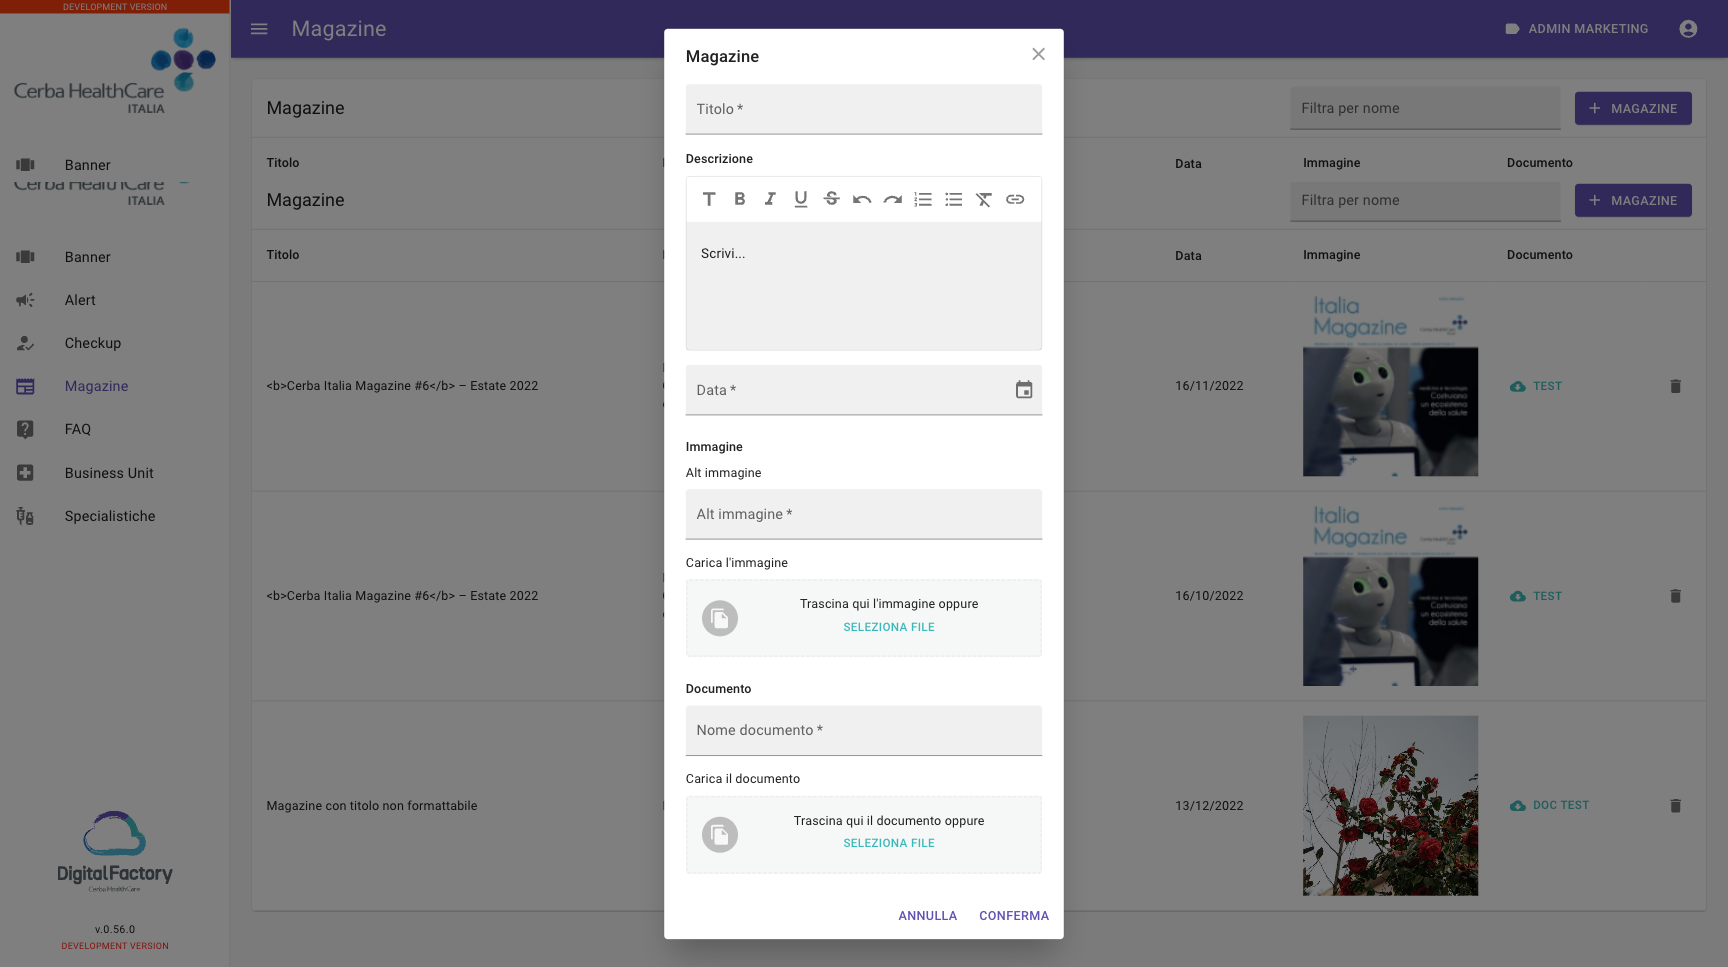
\includegraphics[width=0.7\textwidth]{images/capitolo5/f6_magazines/ModalMagazine_create.png} 
    \caption{Modale aggiunta nuovo magazine} 
    \label{fig:ModalMagazine_create}
\end{figure}

\begin{figure}[H]
    \centering
    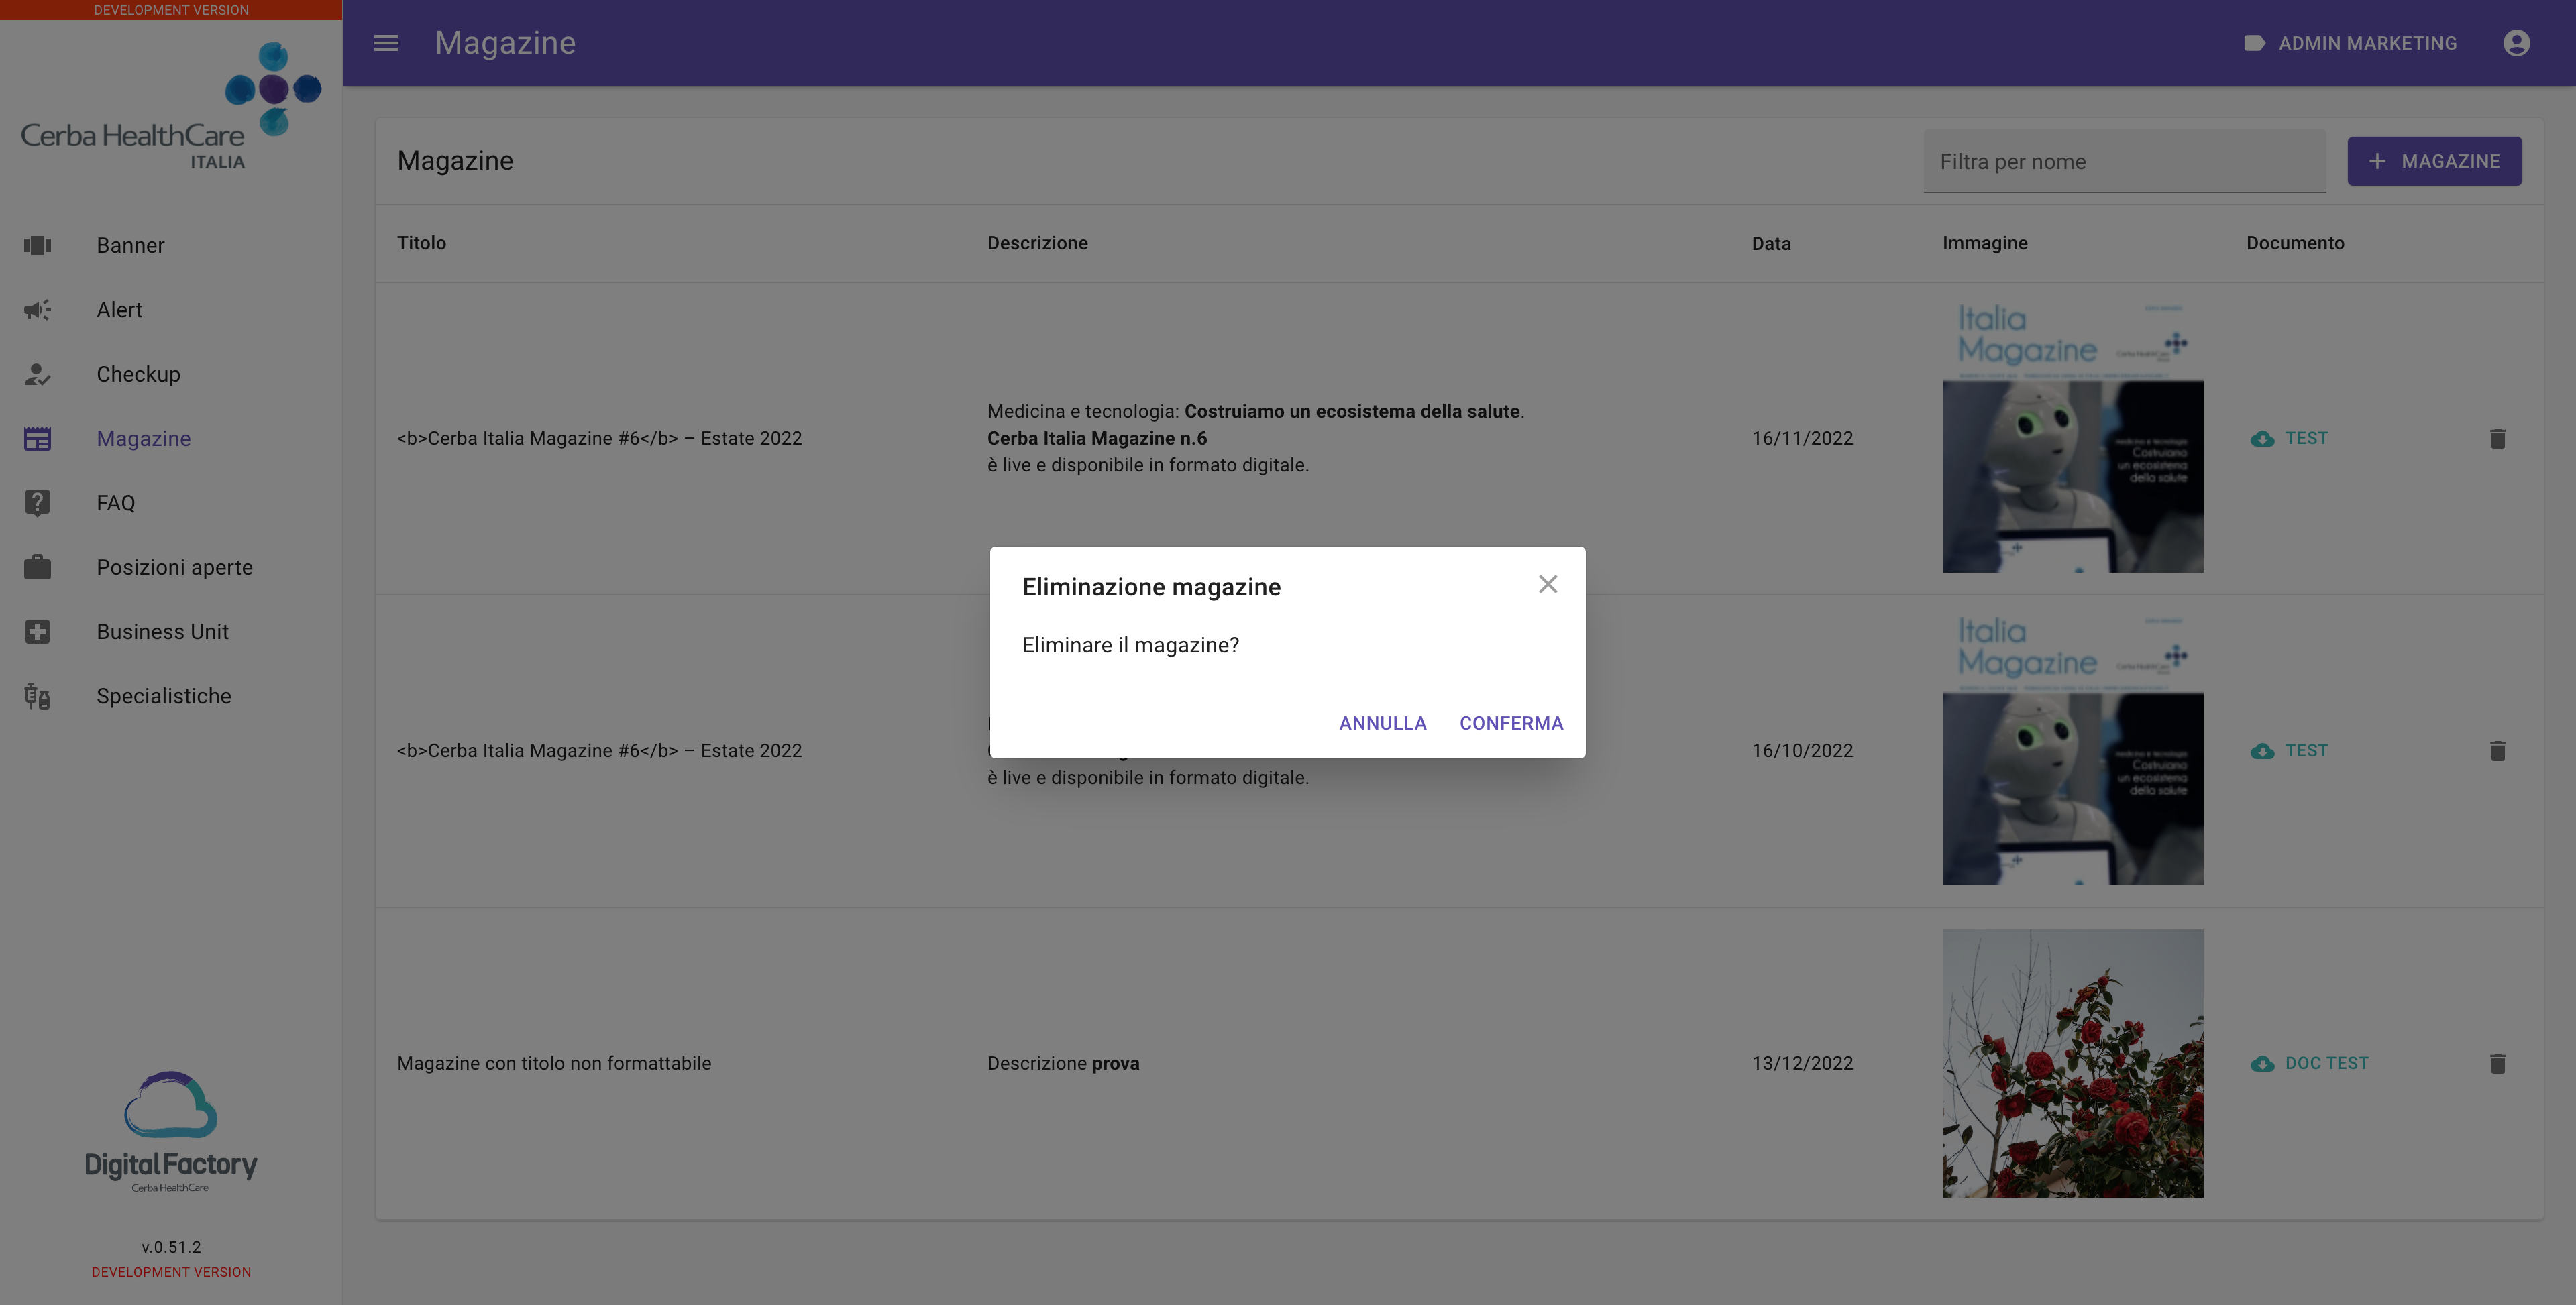
\includegraphics[width=0.75\textwidth]{images/capitolo5/f6_magazines/ModalMagazine_delete.png} 
    \caption{Modale eliminazione magazine esistente} 
    \label{fig:ModalMagazine_delete}
\end{figure}

\begin{figure}[H]
    \centering
    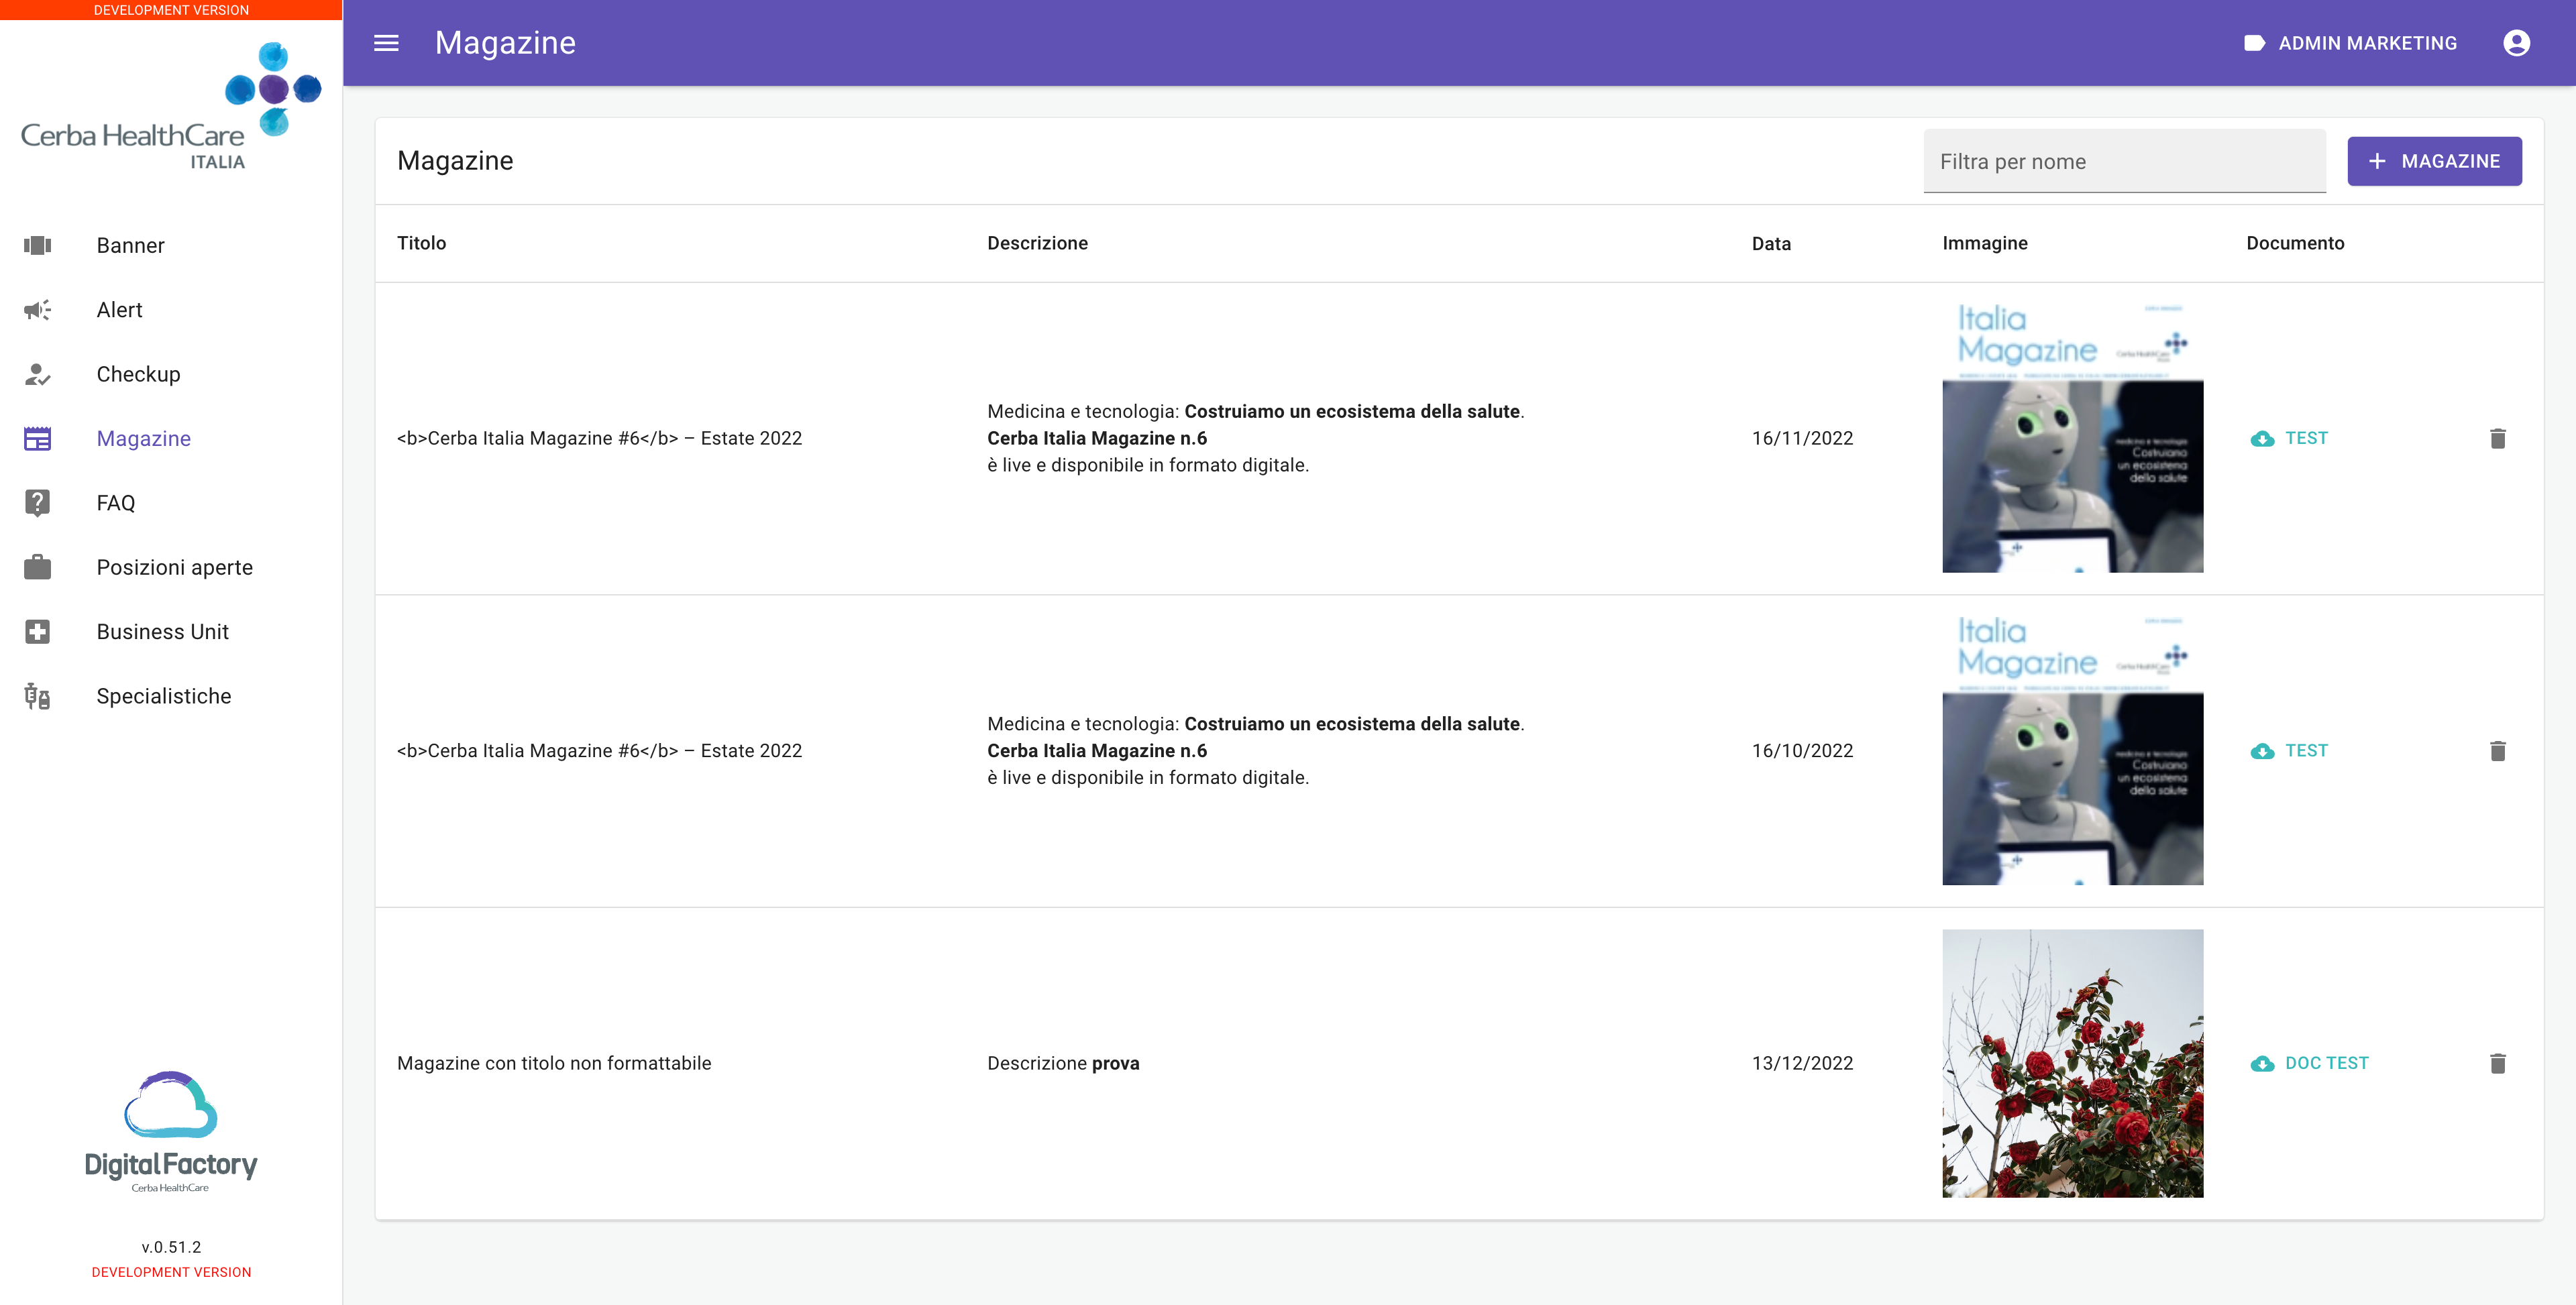
\includegraphics[width=0.75\textwidth]{images/capitolo5/f6_magazines/PageMagazines_searchEmpty.png} 
    \caption{Tabella magazine campo ricerca vuoto} 
    \label{fig:PageMagazine_searchEmpty}
\end{figure}

\begin{figure}[H]
    \centering
    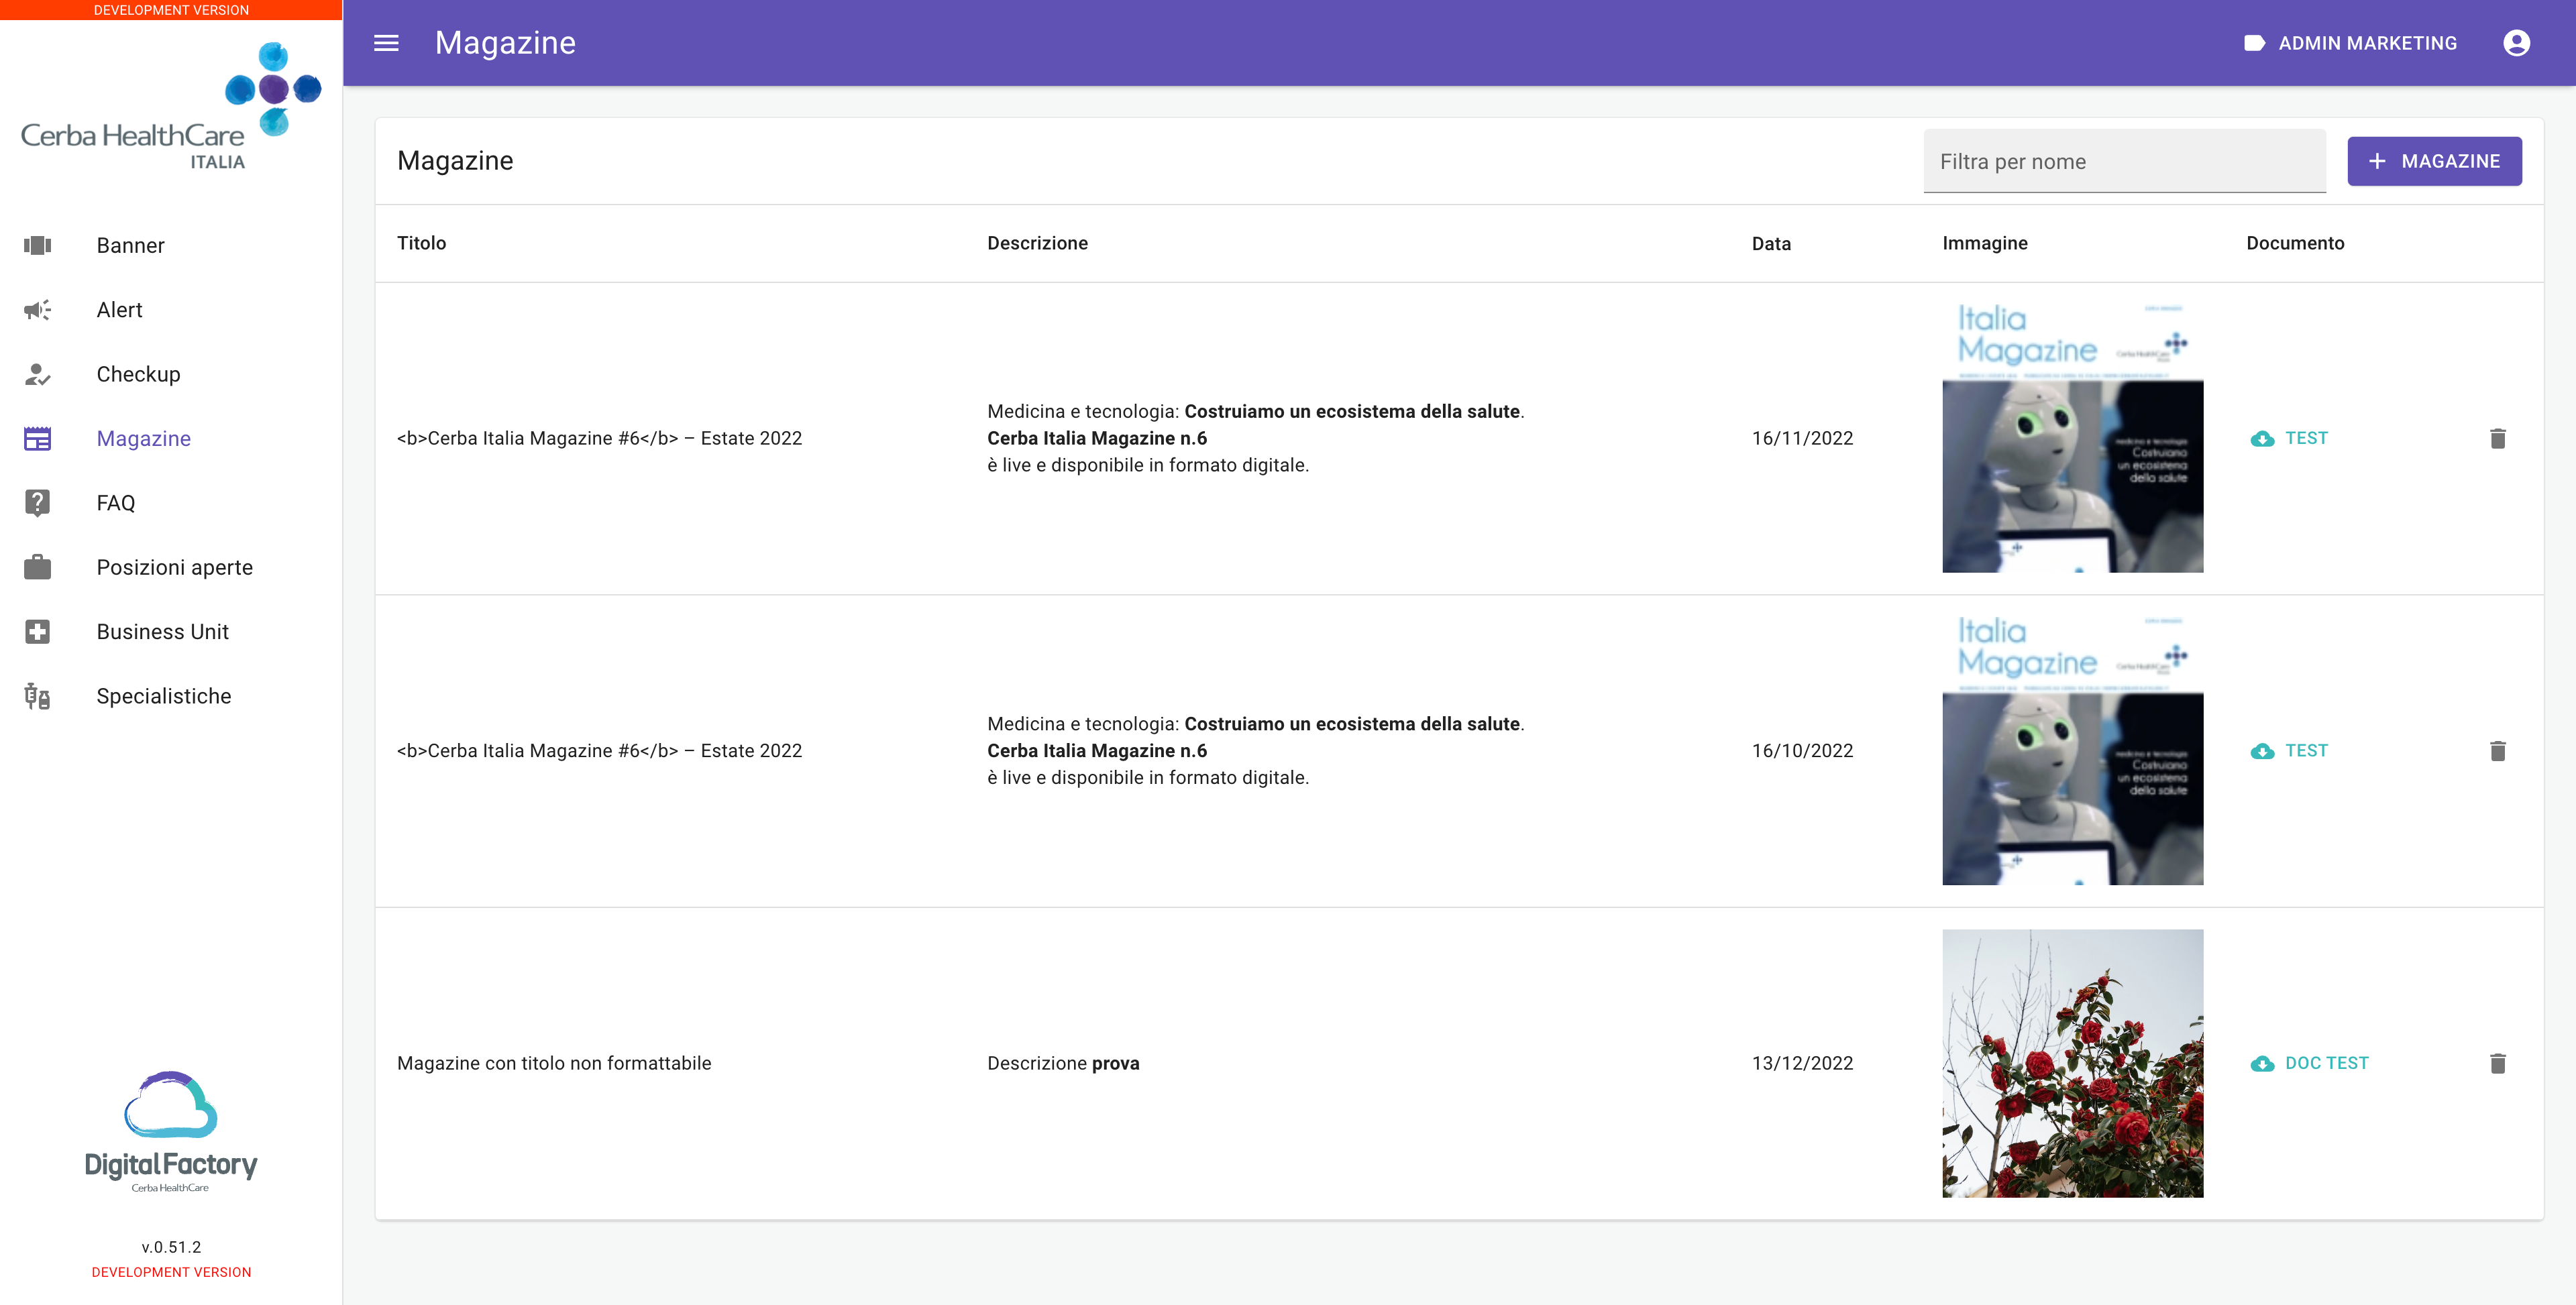
\includegraphics[width=0.75\textwidth]{images/capitolo5/f6_magazines/PageMagazines_searchEmpty.png} 
    \caption{Tabella magazine campo ricerca riempito} 
    \label{fig:PageMagazine_searchFilled}
\end{figure}

\subsection{F7: “FAQ”}
\subparagraph{Requisiti}
Aggiungere la sezione “FAQ” fra quelle previste per il ruolo utente \textit{marketing admin}.\\
Al suo interno, una tabella deve mostrare le FAQ esistenti in una lista semplice e riportarne le proprietà “Domanda”, “Risposta” e “Categoria”.\\
Deve essere possibile aggiungere, modificare o eliminare una FAQ.\\
Solamente per la proprietà “Risposta” deve essere fornita la possibilità di formattare il testo.\\
L'\textit{header} della tabella delle FAQ deve essere dotato di un campo di ricerca. Questo deve essere in grado di filtrare per domanda e posizionato alla sinistra del bottone per l'aggiunta di una nuova FAQ.

% \paragraph{\textit{Output} grafico}
% \begin{figure}[H]
%     \centering
%     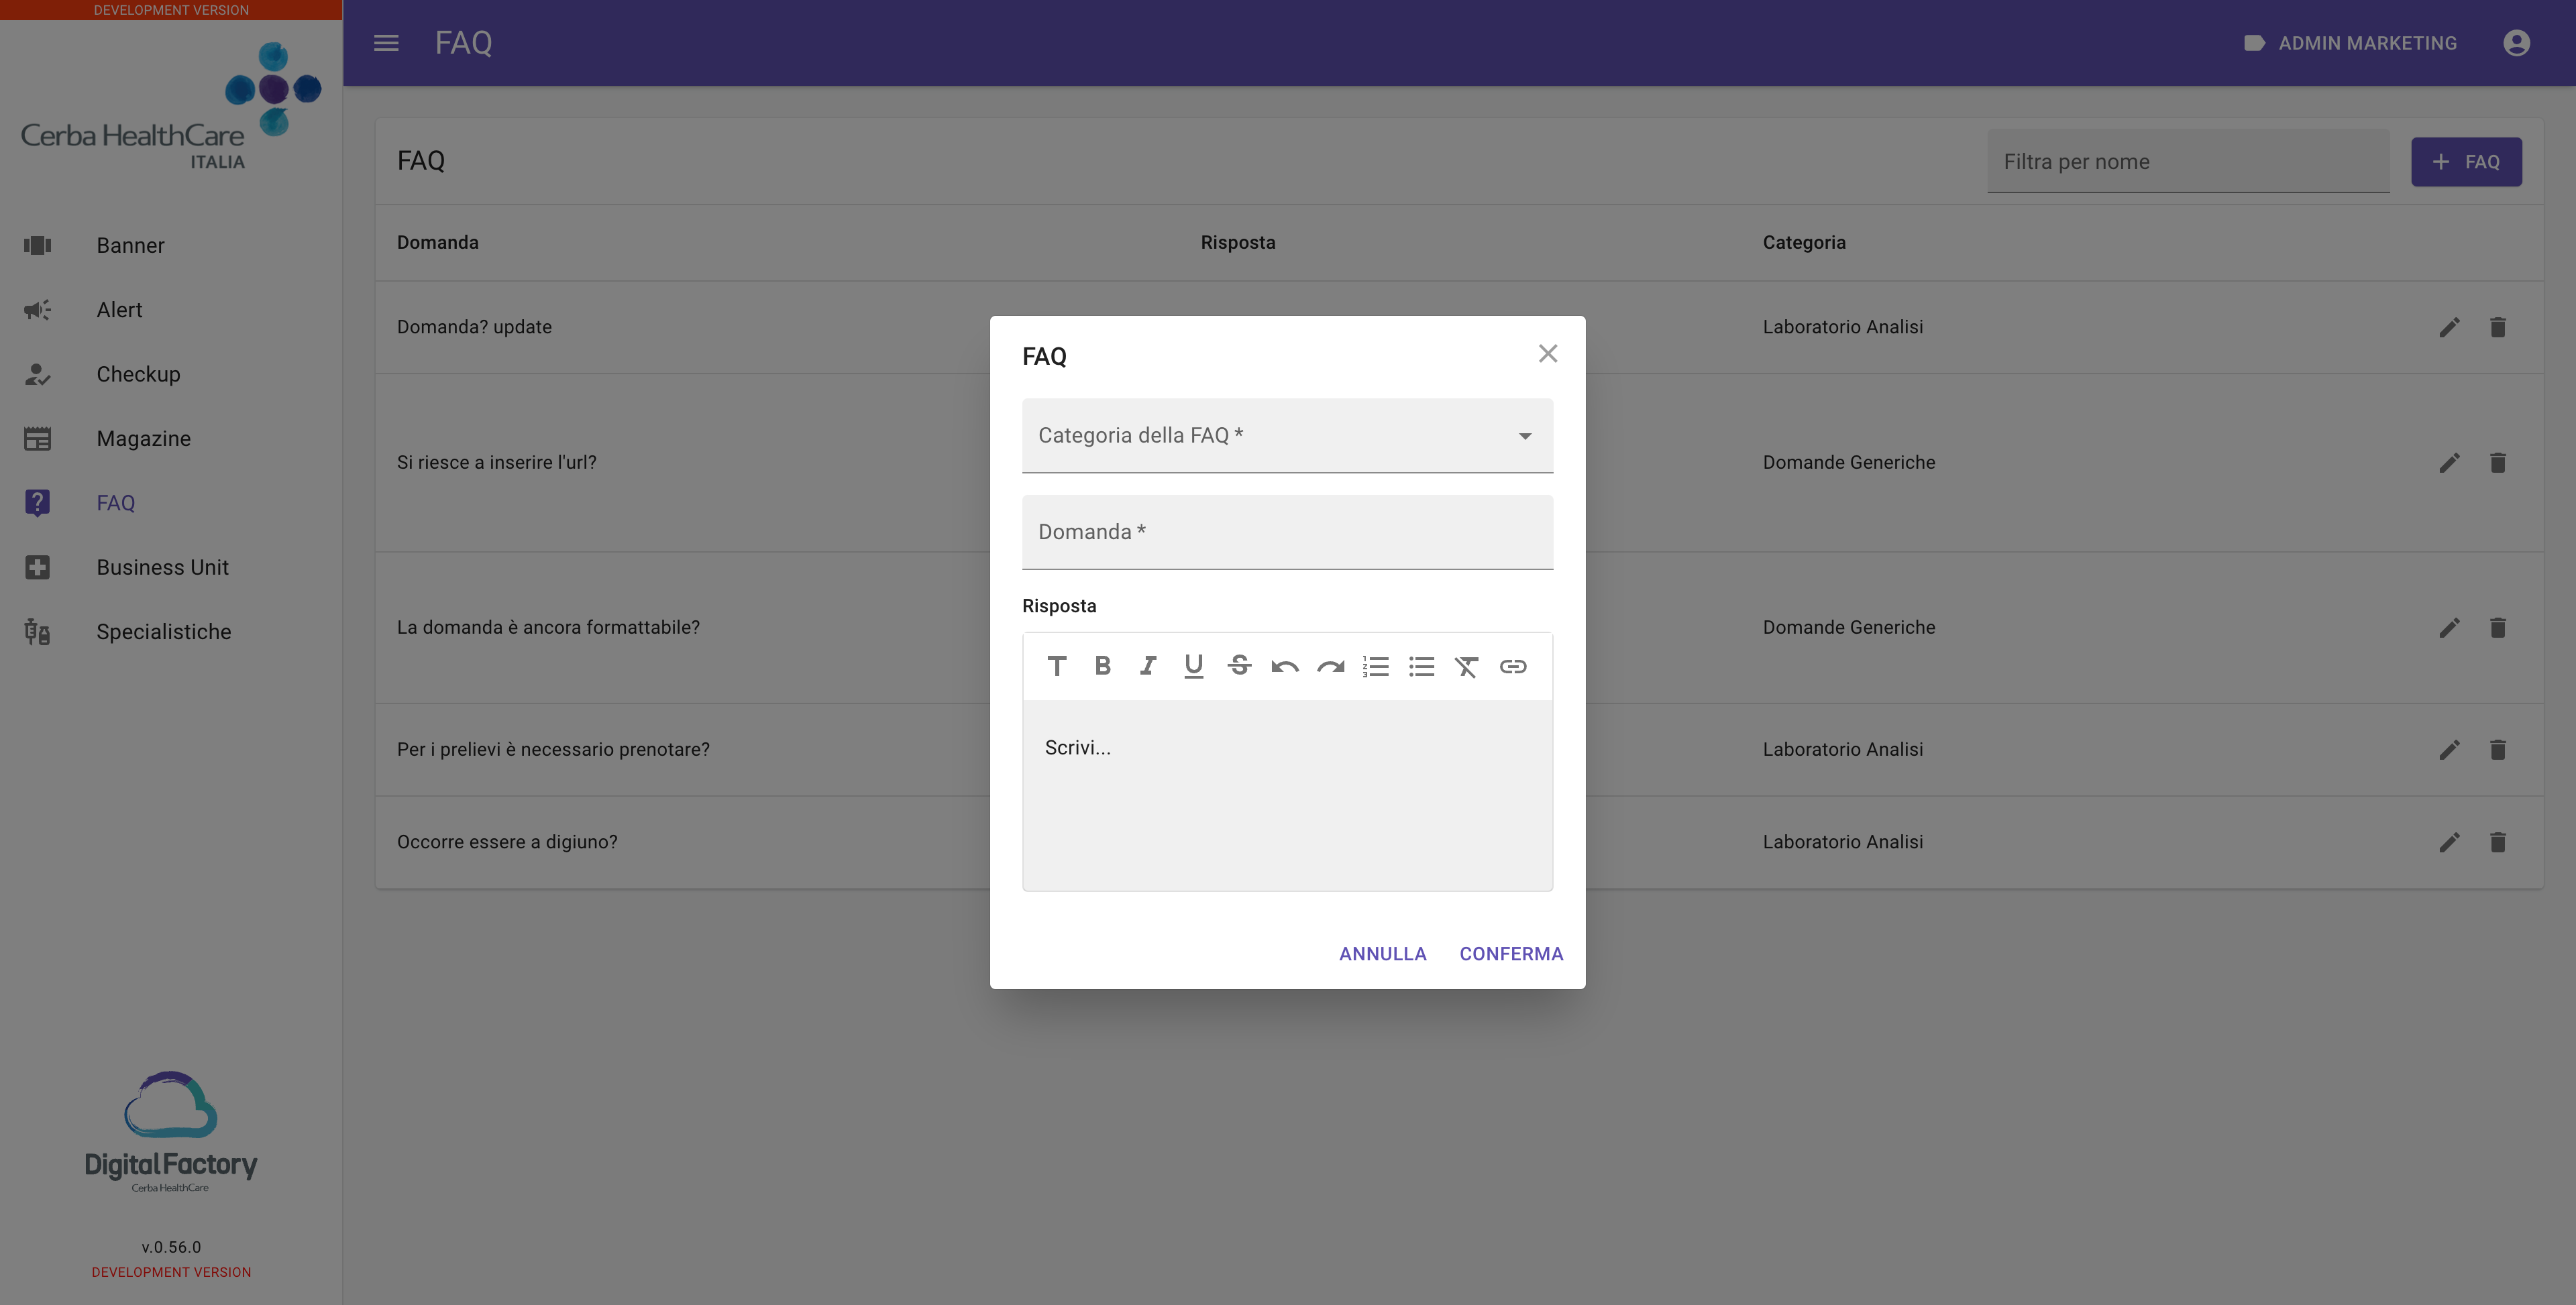
\includegraphics[width=0.75\textwidth]{images/capitolo5/f7_faqs/ModalFaq_create.png} 
%     \caption{Modale aggiunta nuova faq} 
%     \label{fig:ModalFaq_create}
% \end{figure}

% \begin{figure}[H]
%     \centering
%     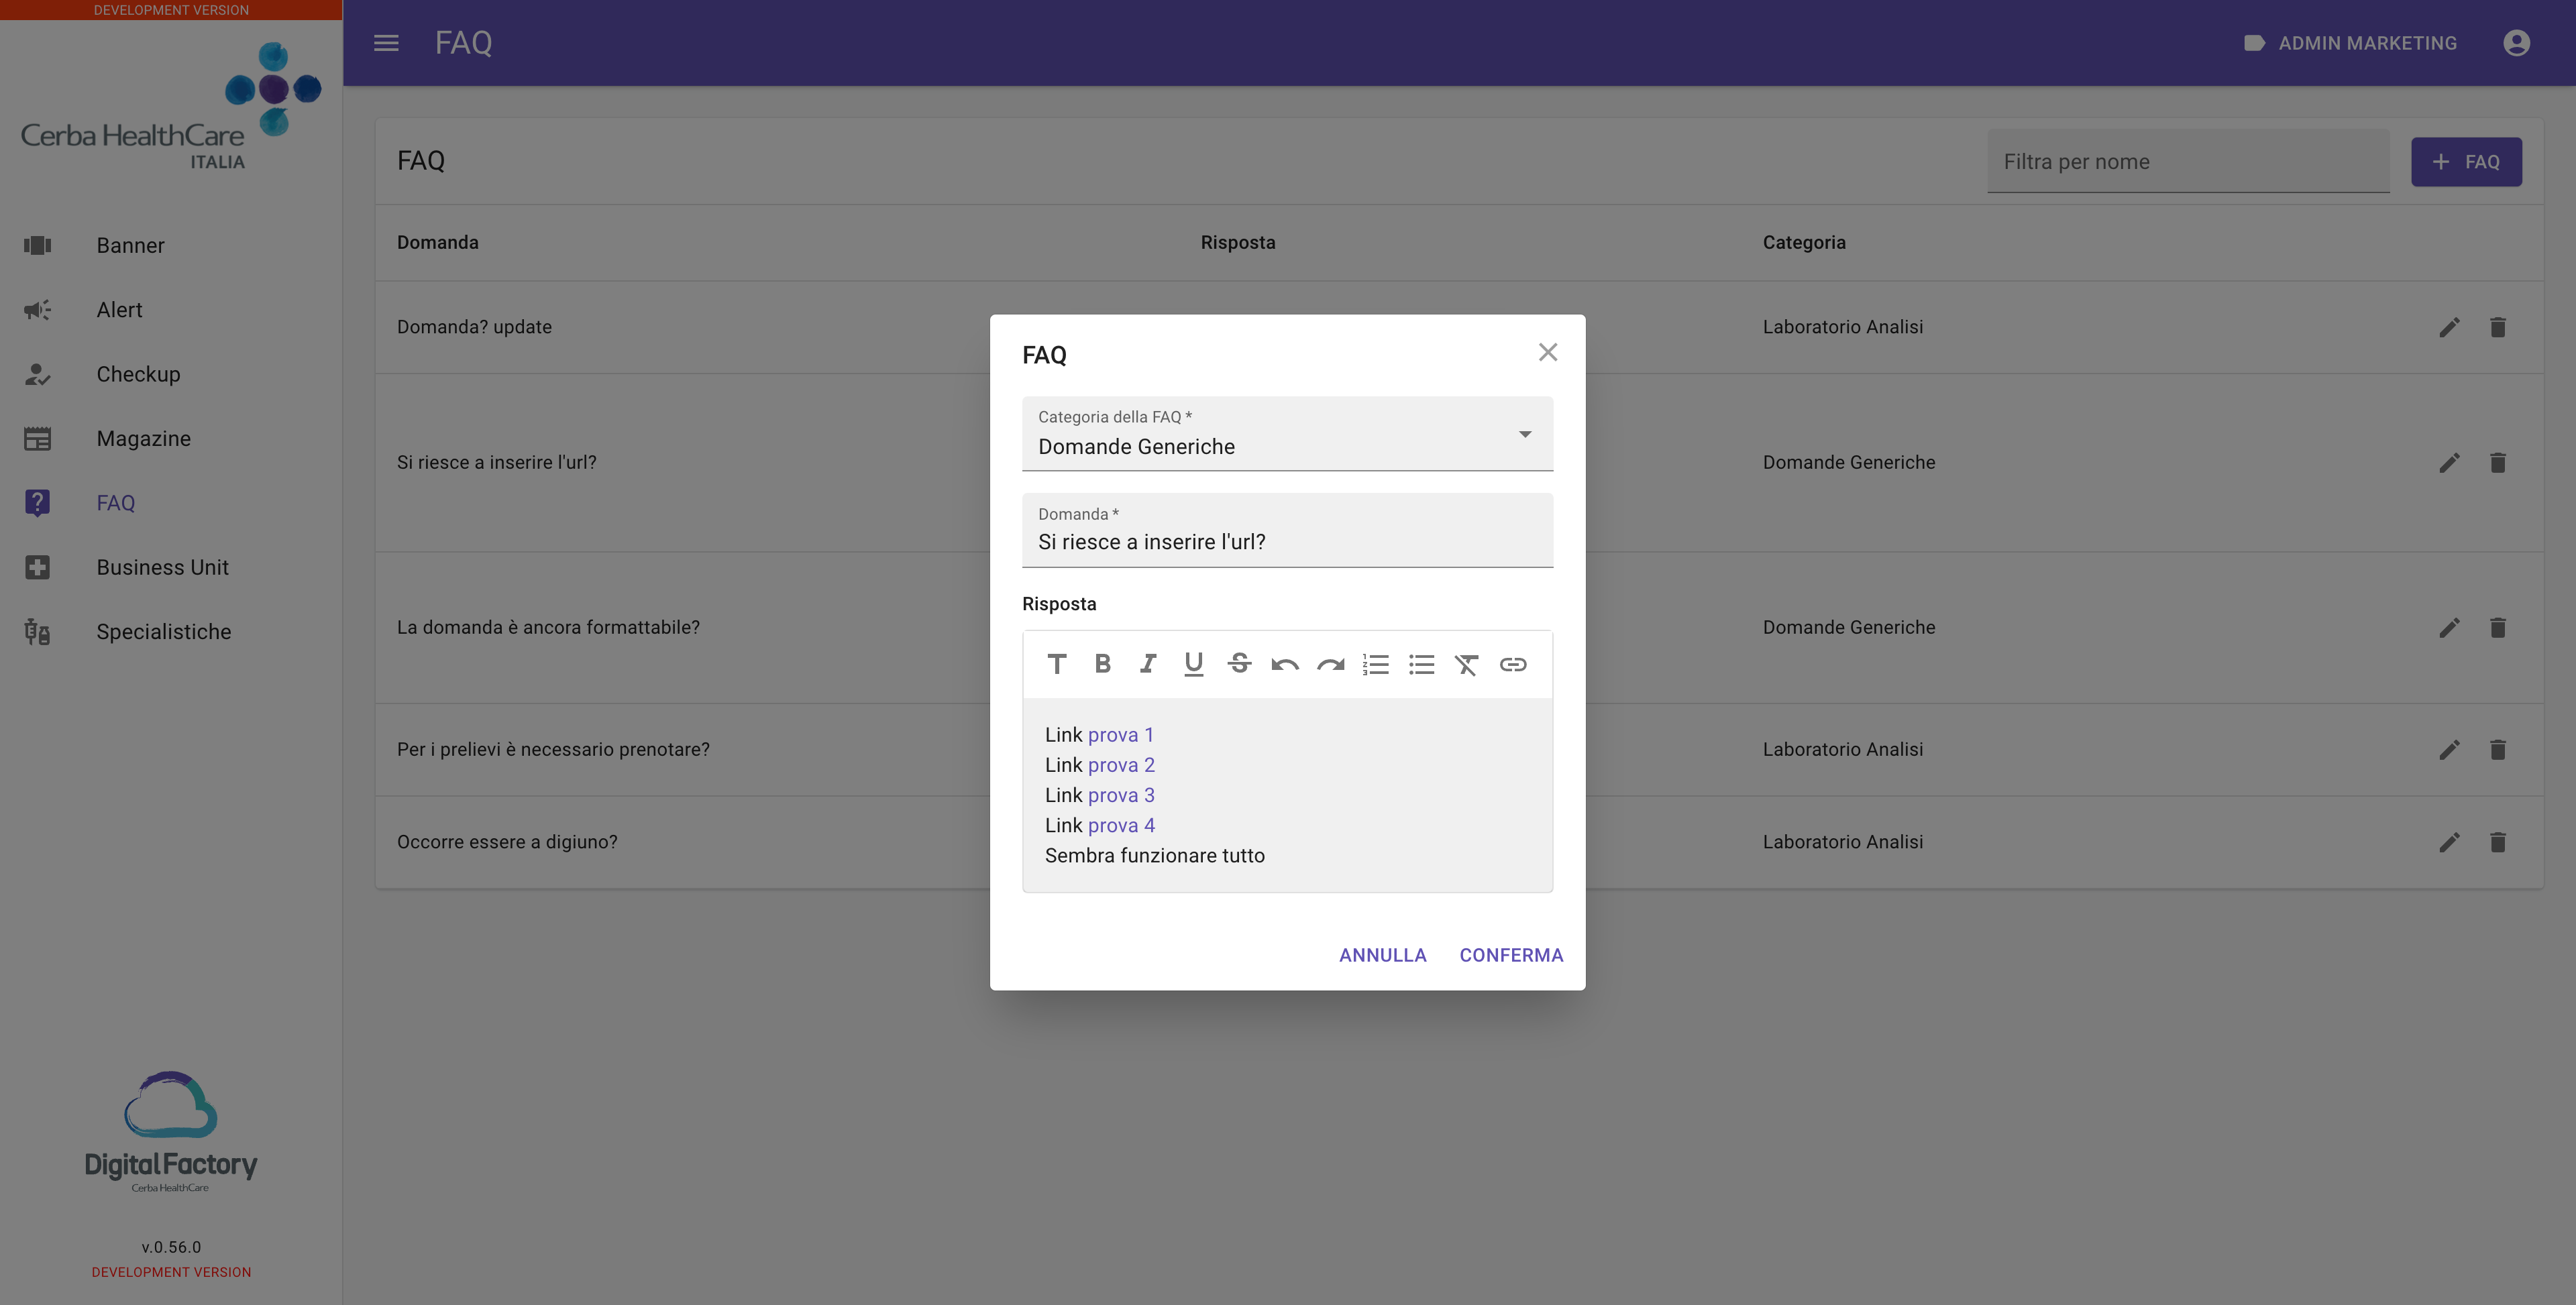
\includegraphics[width=0.75\textwidth]{images/capitolo5/f7_faqs/ModalFaq_edit.png} 
%     \caption{Modale modifica faq esistente} 
%     \label{fig:ModalFaq_edit}
% \end{figure}

% \begin{figure}[H]
%     \centering
%     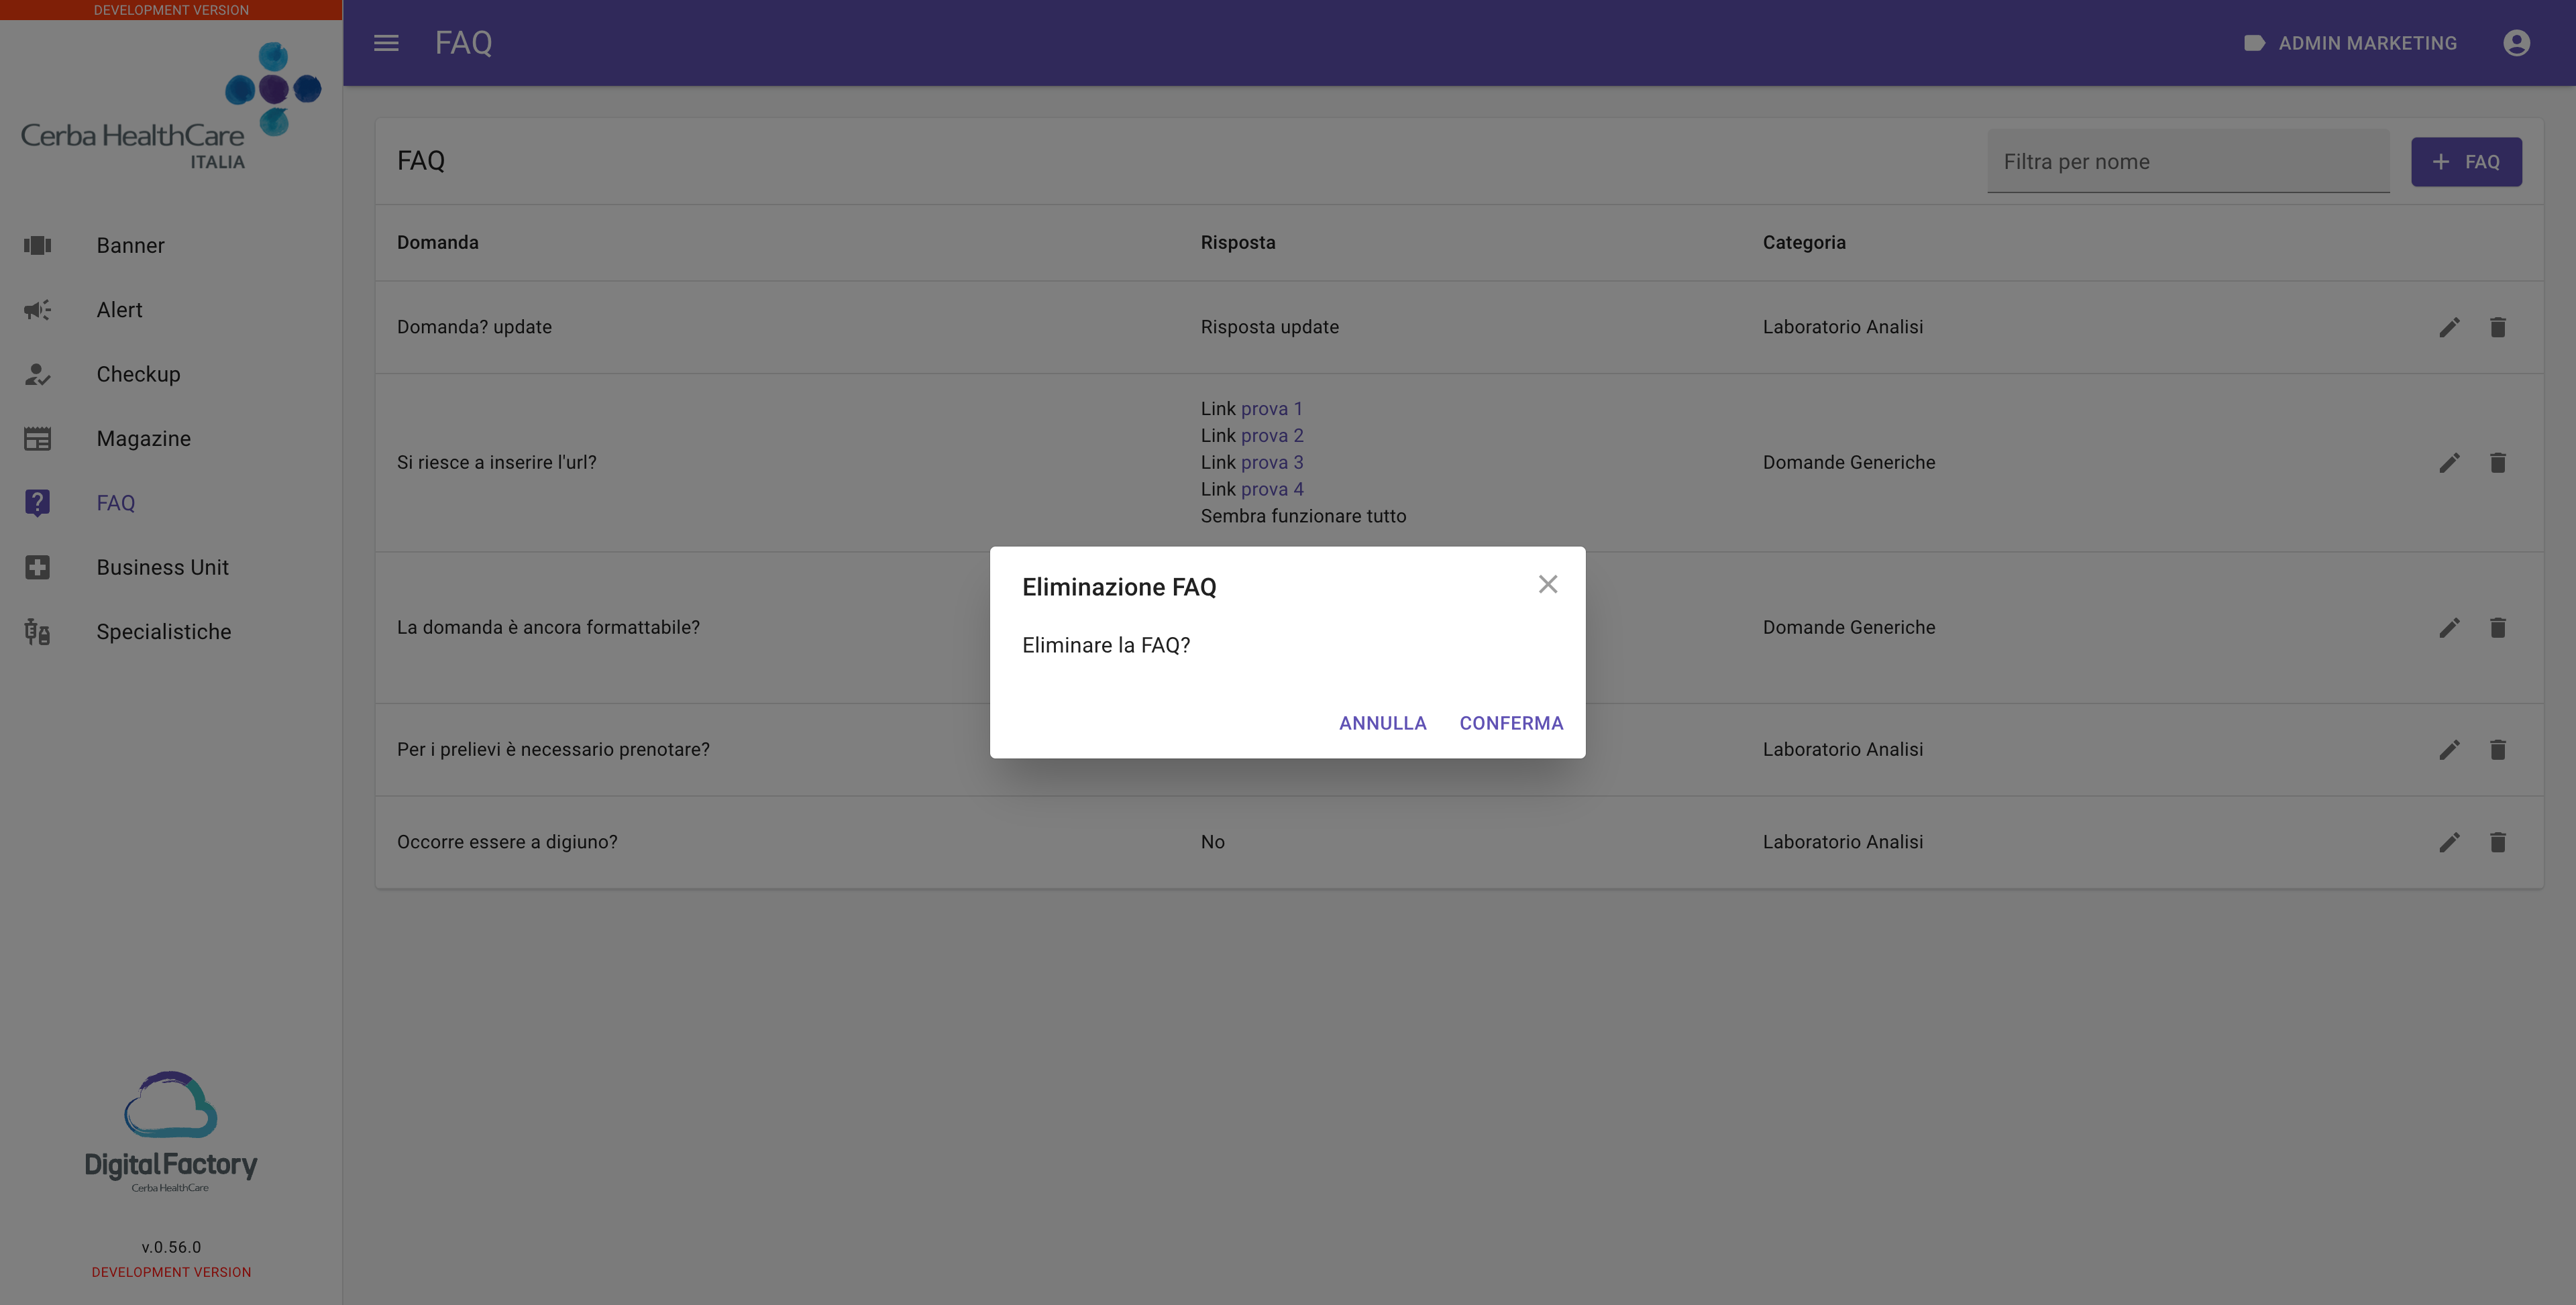
\includegraphics[width=0.75\textwidth]{images/capitolo5/f7_faqs/ModalFaq_delete.png} 
%     \caption{Modale eliminazione faq esistente} 
%     \label{fig:ModalFaq_edit}
% \end{figure}

% \begin{figure}[H]
%     \centering
%     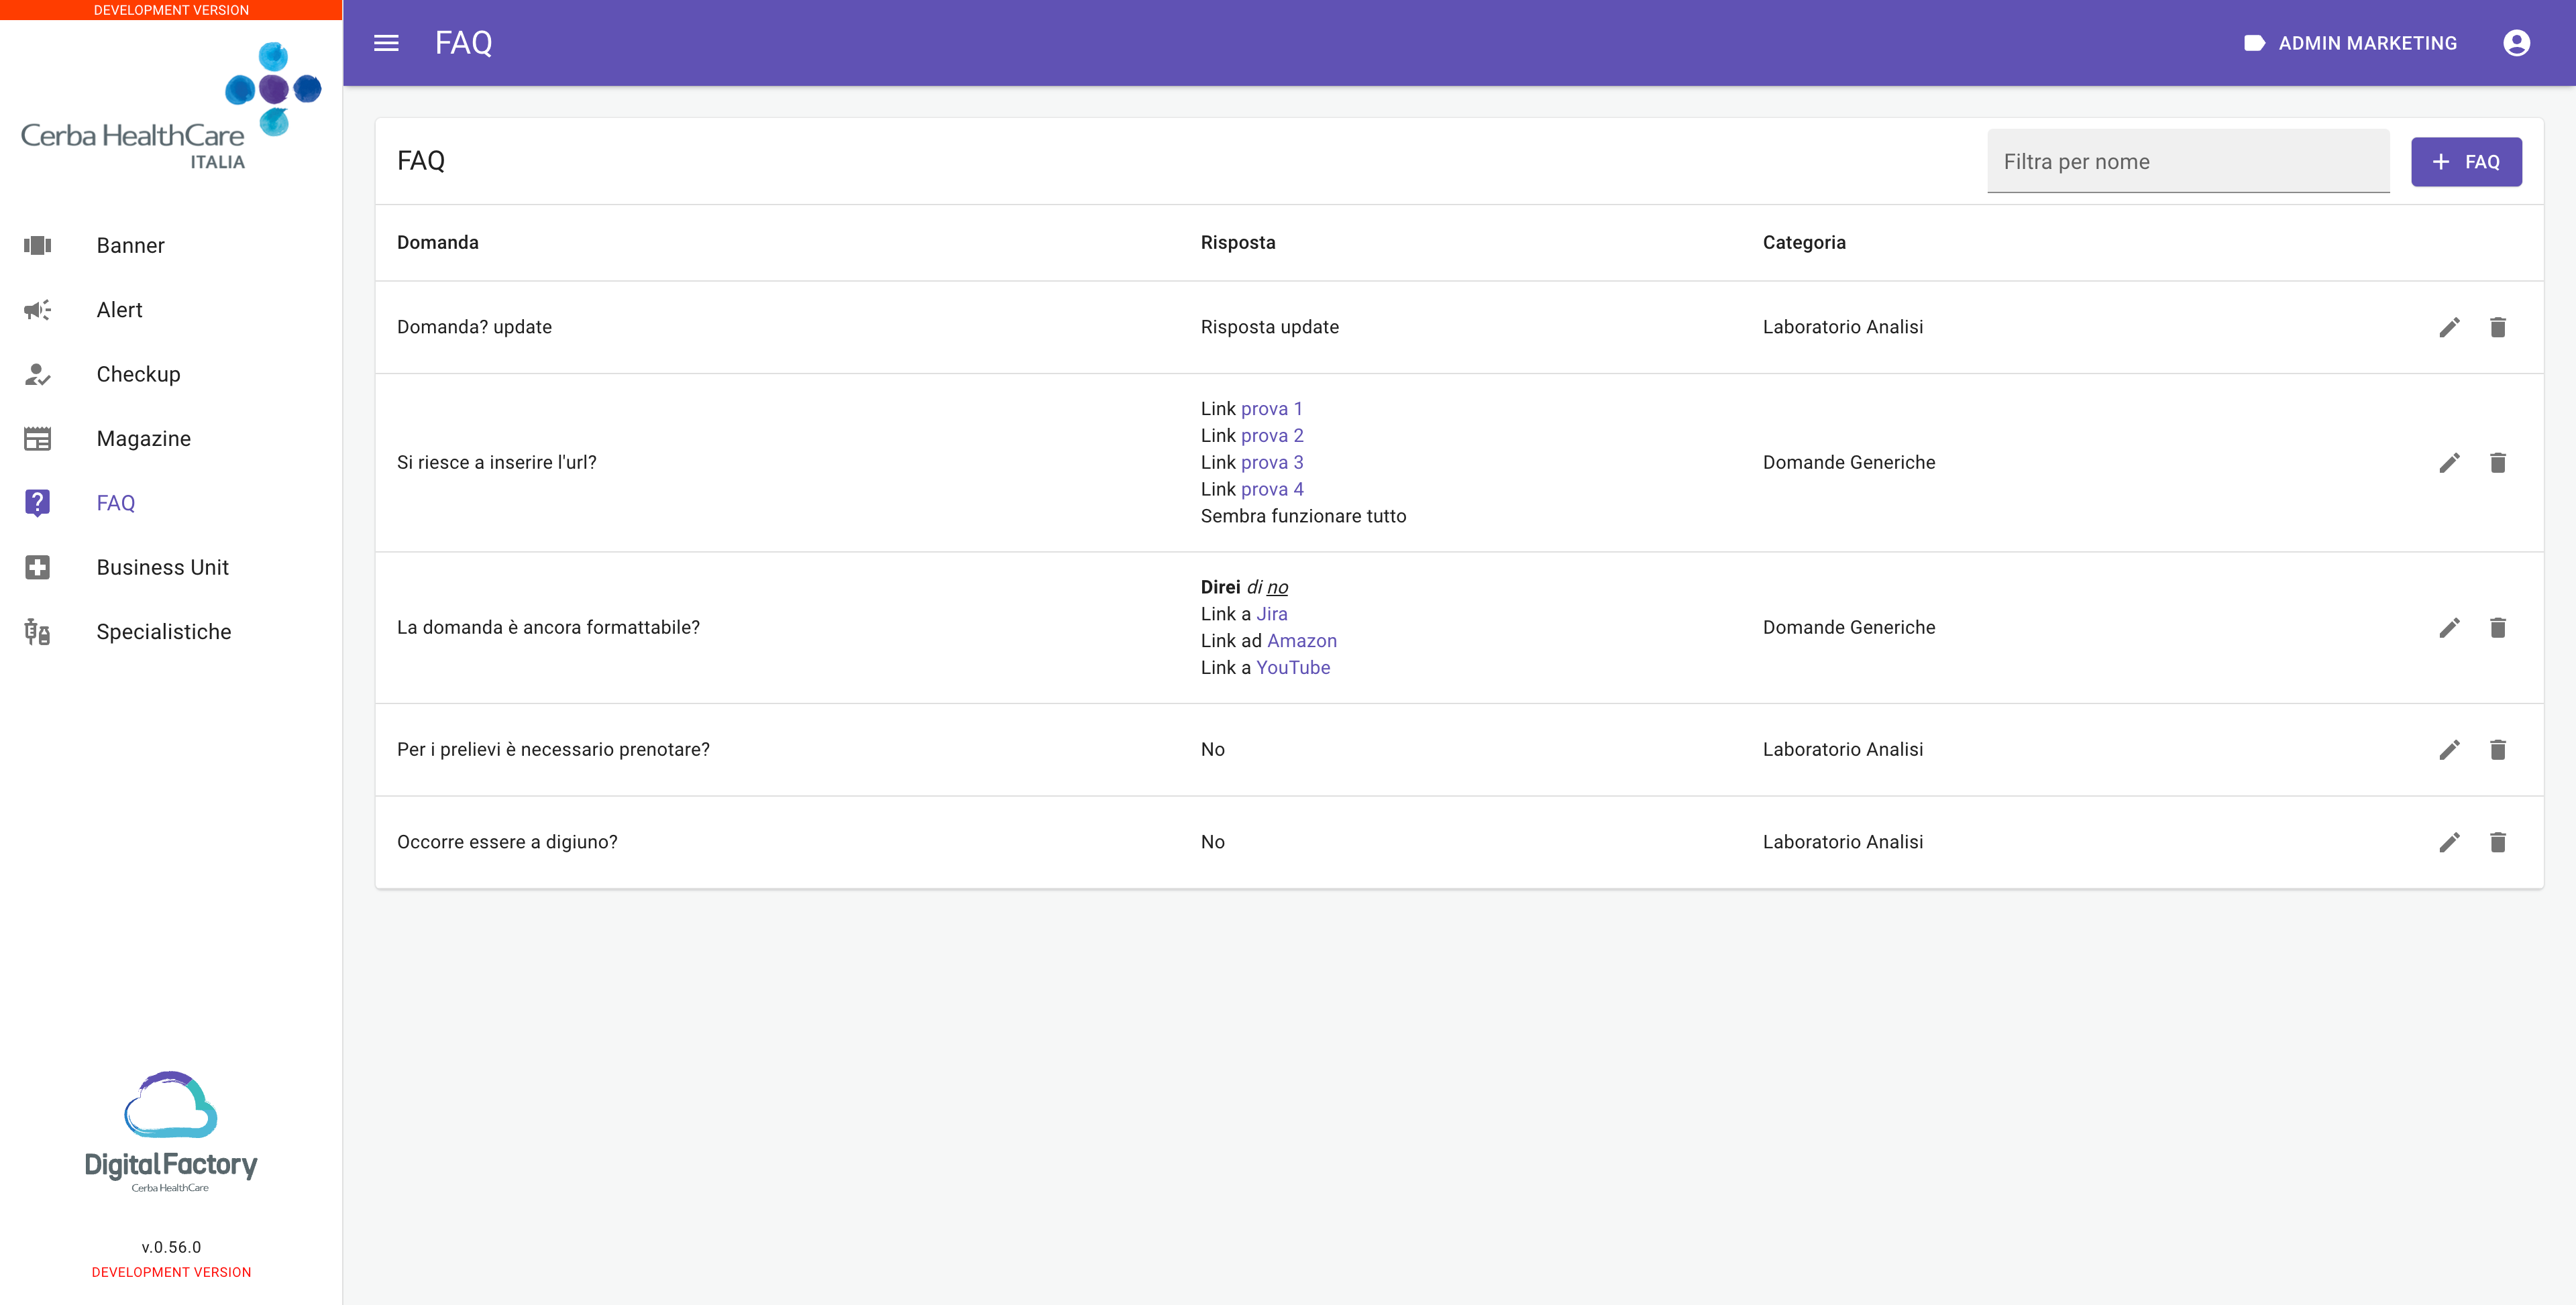
\includegraphics[width=0.75\textwidth]{images/capitolo5/f7_faqs/PageFaq_searchEmpty.png} 
%     \caption{Tabella faq campo ricerca vuoto} 
%     \label{fig:PageFaq_searchEmpty}
% \end{figure}

% \begin{figure}[H]
%     \centering
%     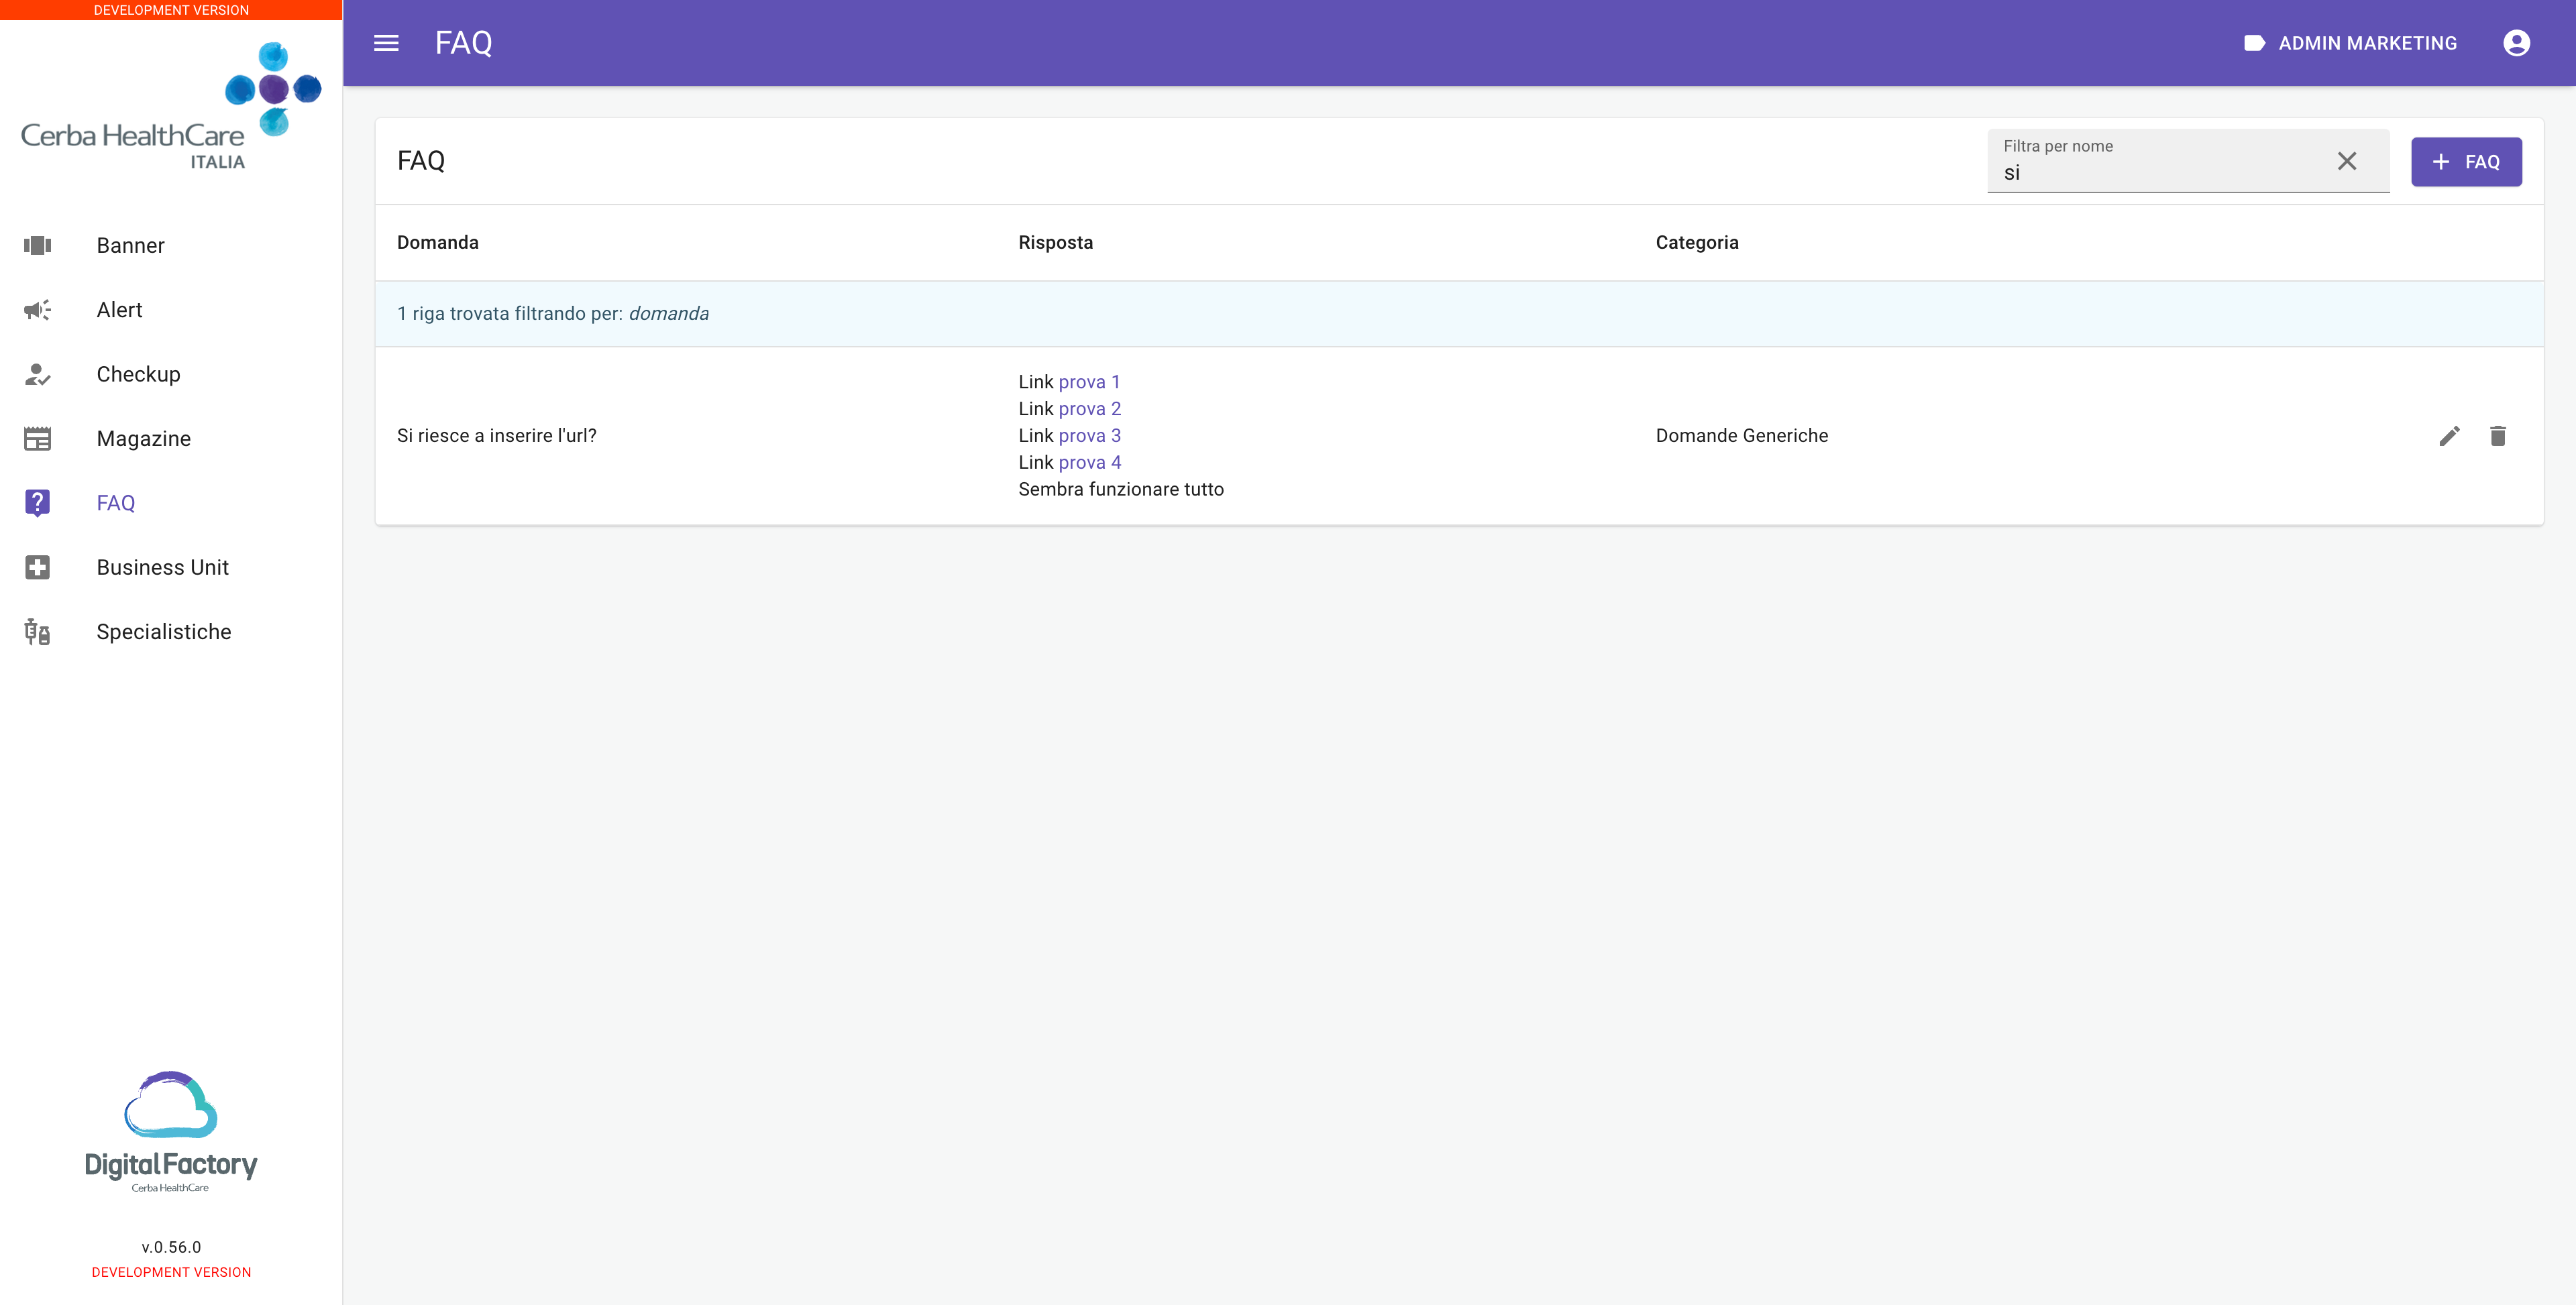
\includegraphics[width=0.75\textwidth]{images/capitolo5/f7_faqs/PageFaq_searchFilled.png} 
%     \caption{Tabella faq campo ricerca riempito} 
%     \label{fig:PageFaq_searchFilled}
% \end{figure}

\subsection{F8: “Business Unit”}
\subparagraph{Requisiti}
Aggiungere la sezione “Business Unit” fra quelle previste per il ruolo utente \textit{marketing admin}.\\
Al suo interno, una tabella deve mostrare le \textit{business unit} (BU) esistenti in una lista semplice e riportarne la proprietà “Nome”.\\
L'\textit{header} della tabella delle BU deve essere dotato di un campo di ricerca. Questo deve essere in grado di filtrare per nome e posizionato all'estrema destra dell'\textit{header} della tabella.\\
Ogni BU deve essere dotata di una pagina di dettaglio alla quale si accede cliccando sul link posto in concomitanza del nome. Qui, deve essere possibile modificare e visualizzare la descrizione, campo che deve poter essere formattato; sempre all'interno della pagina di dettaglio, si devono poter aggiungere, visualizzare ed eliminare un'immagine e un'icona.

\paragraph{\textit{Output} grafico}
\begin{figure}[H]
    \centering
    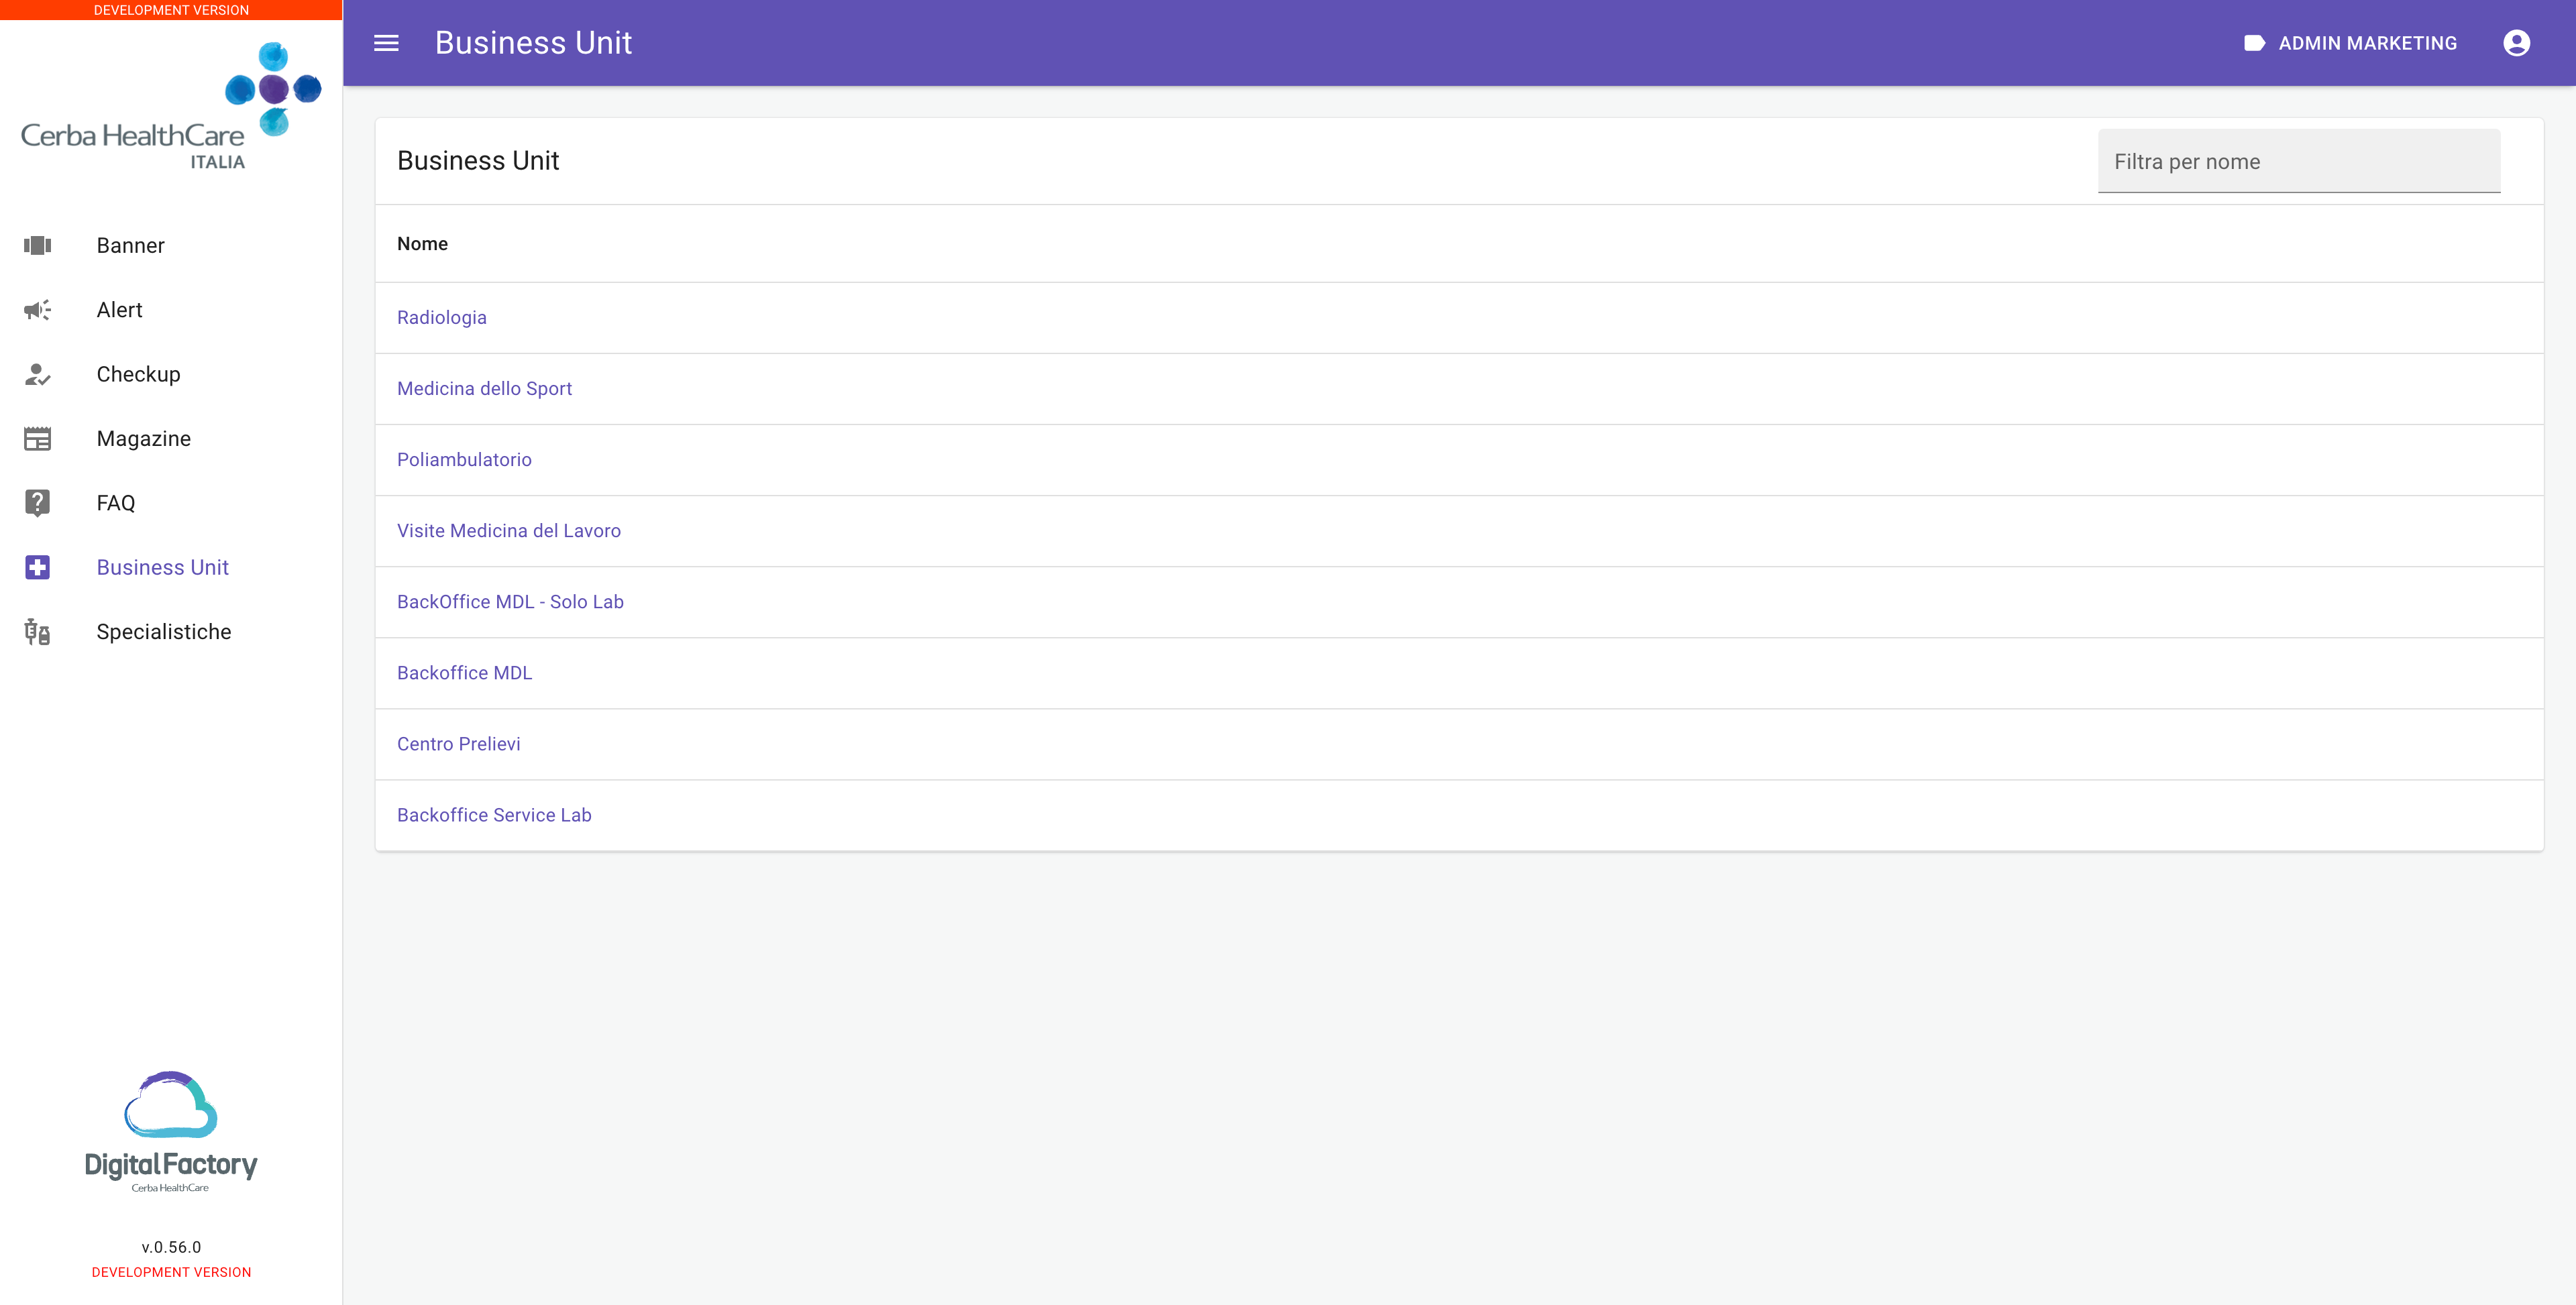
\includegraphics[width=0.75\textwidth]{images/capitolo5/f8_businessUnits/PageBusinessUnits_searchEmpty.png} 
    \caption{Tabella BU campo ricerca vuoto} 
    \label{fig:PageBusinessUnits_searchEmpty}
\end{figure}

\begin{figure}[H]
    \centering
    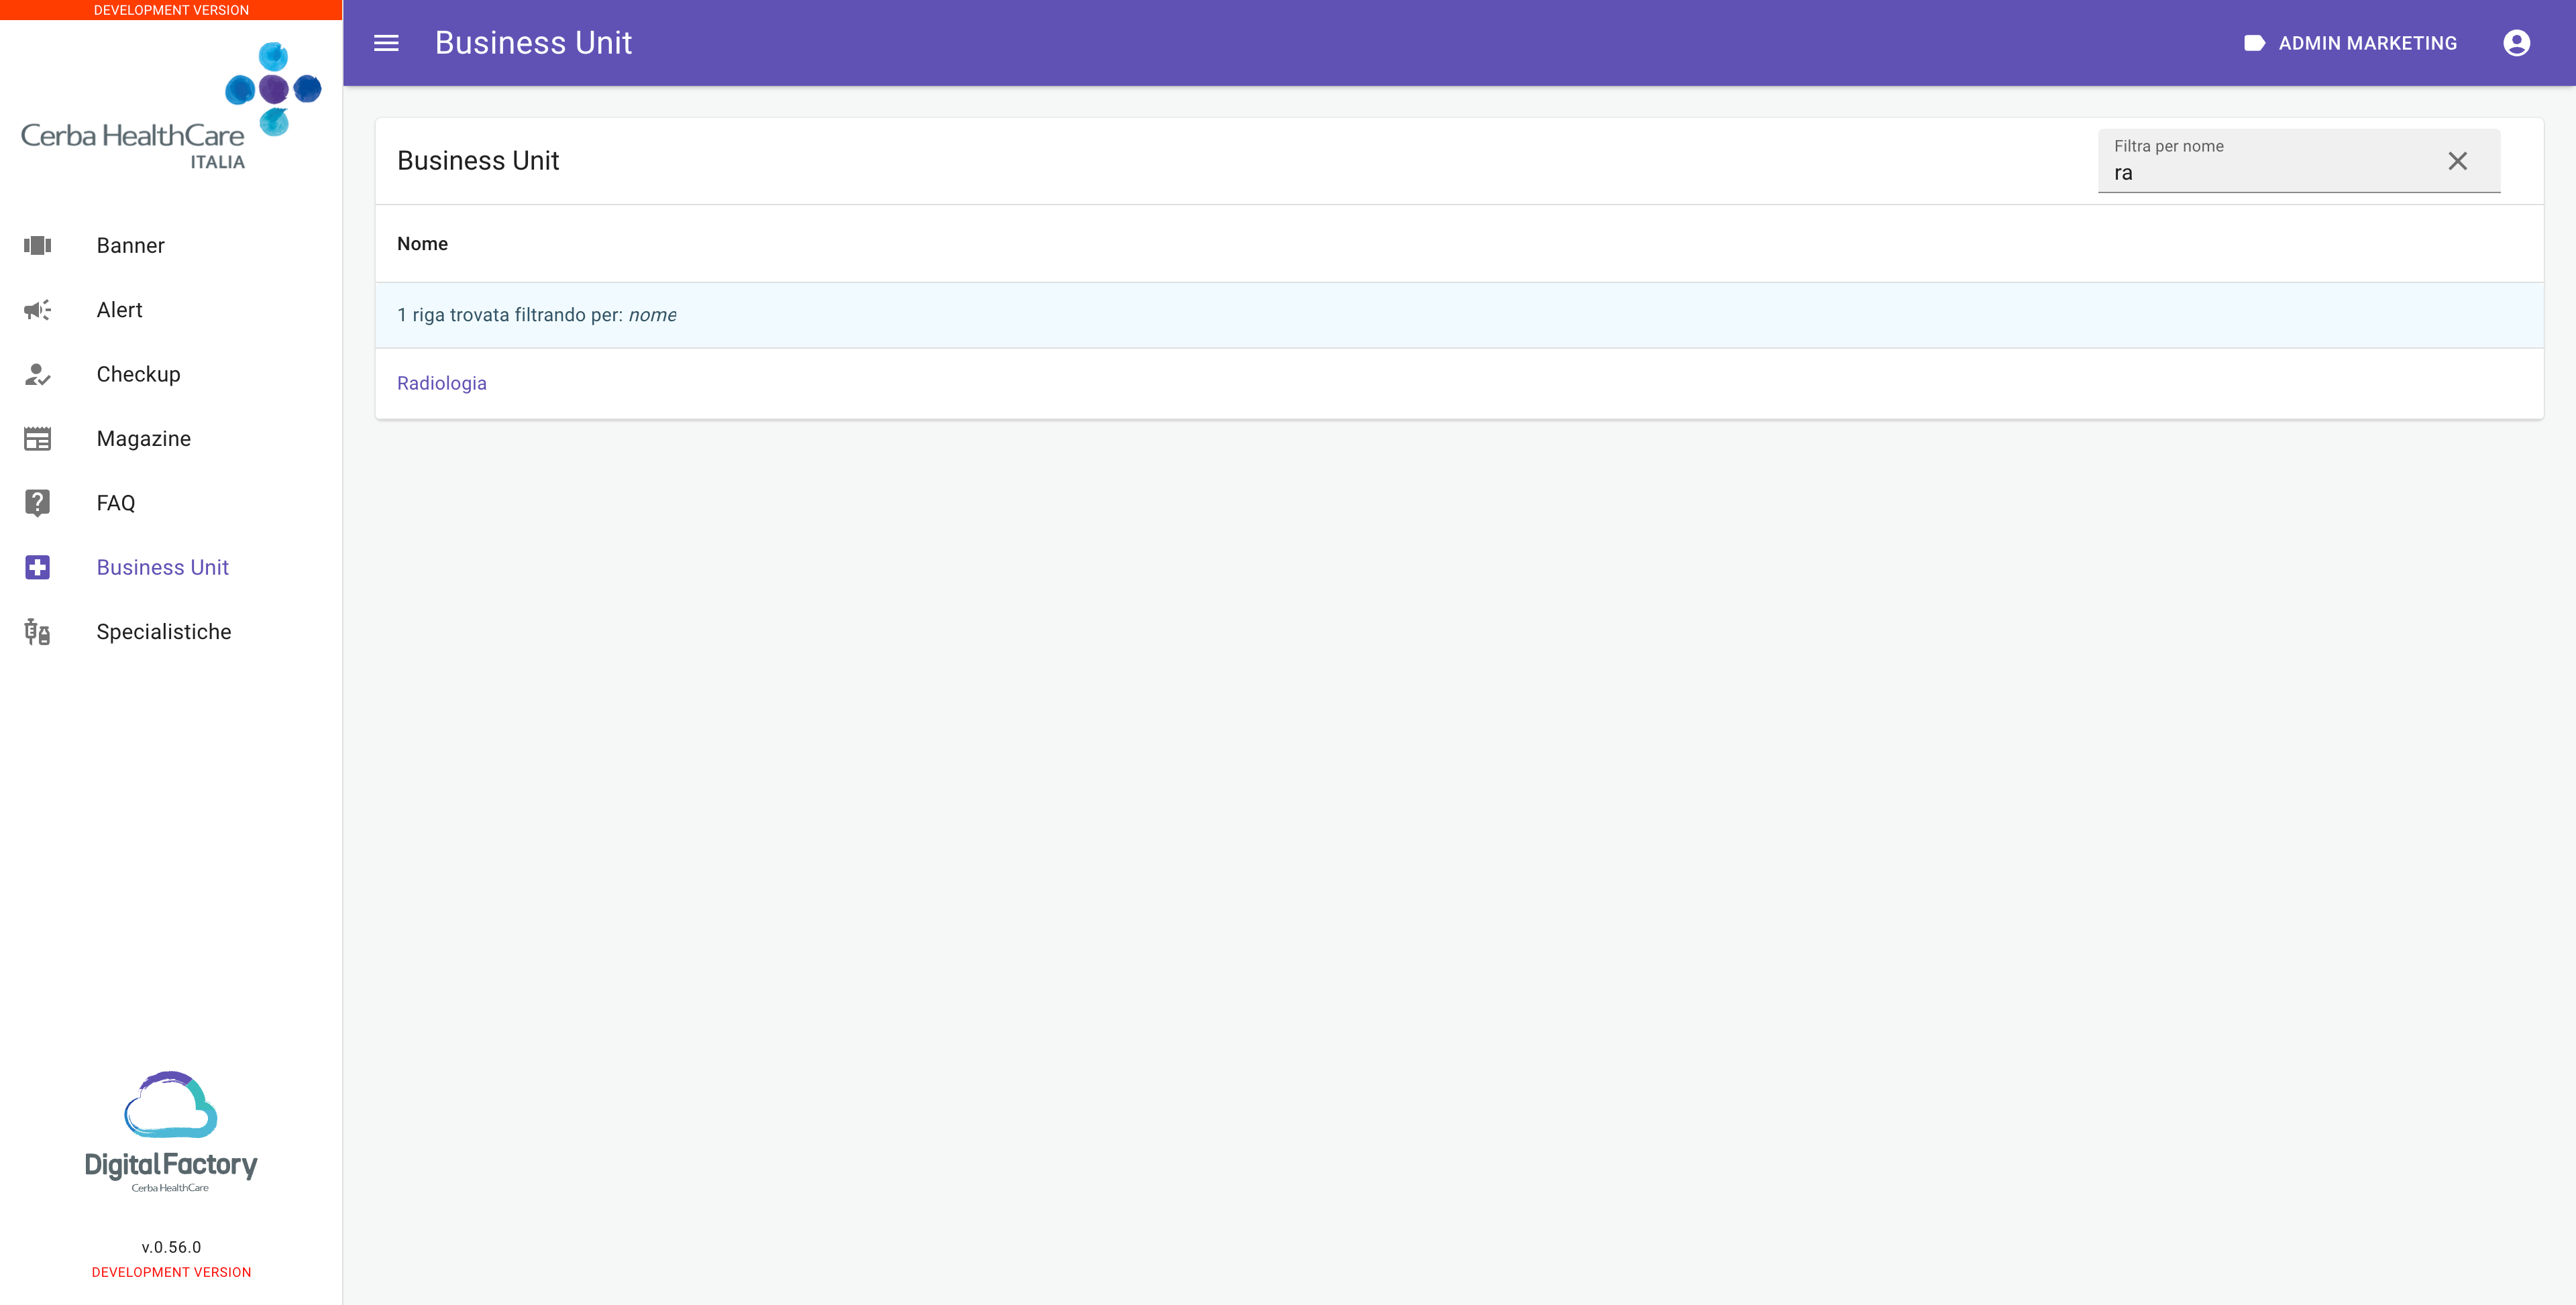
\includegraphics[width=0.75\textwidth]{images/capitolo5/f8_businessUnits/PageBusinessUnits_searchFilled.png} 
    \caption{Tabella BU campo ricerca riempito} 
    \label{fig:PageBusinessUnits_searchFilled}
\end{figure}

\begin{figure}[H]
    \centering
    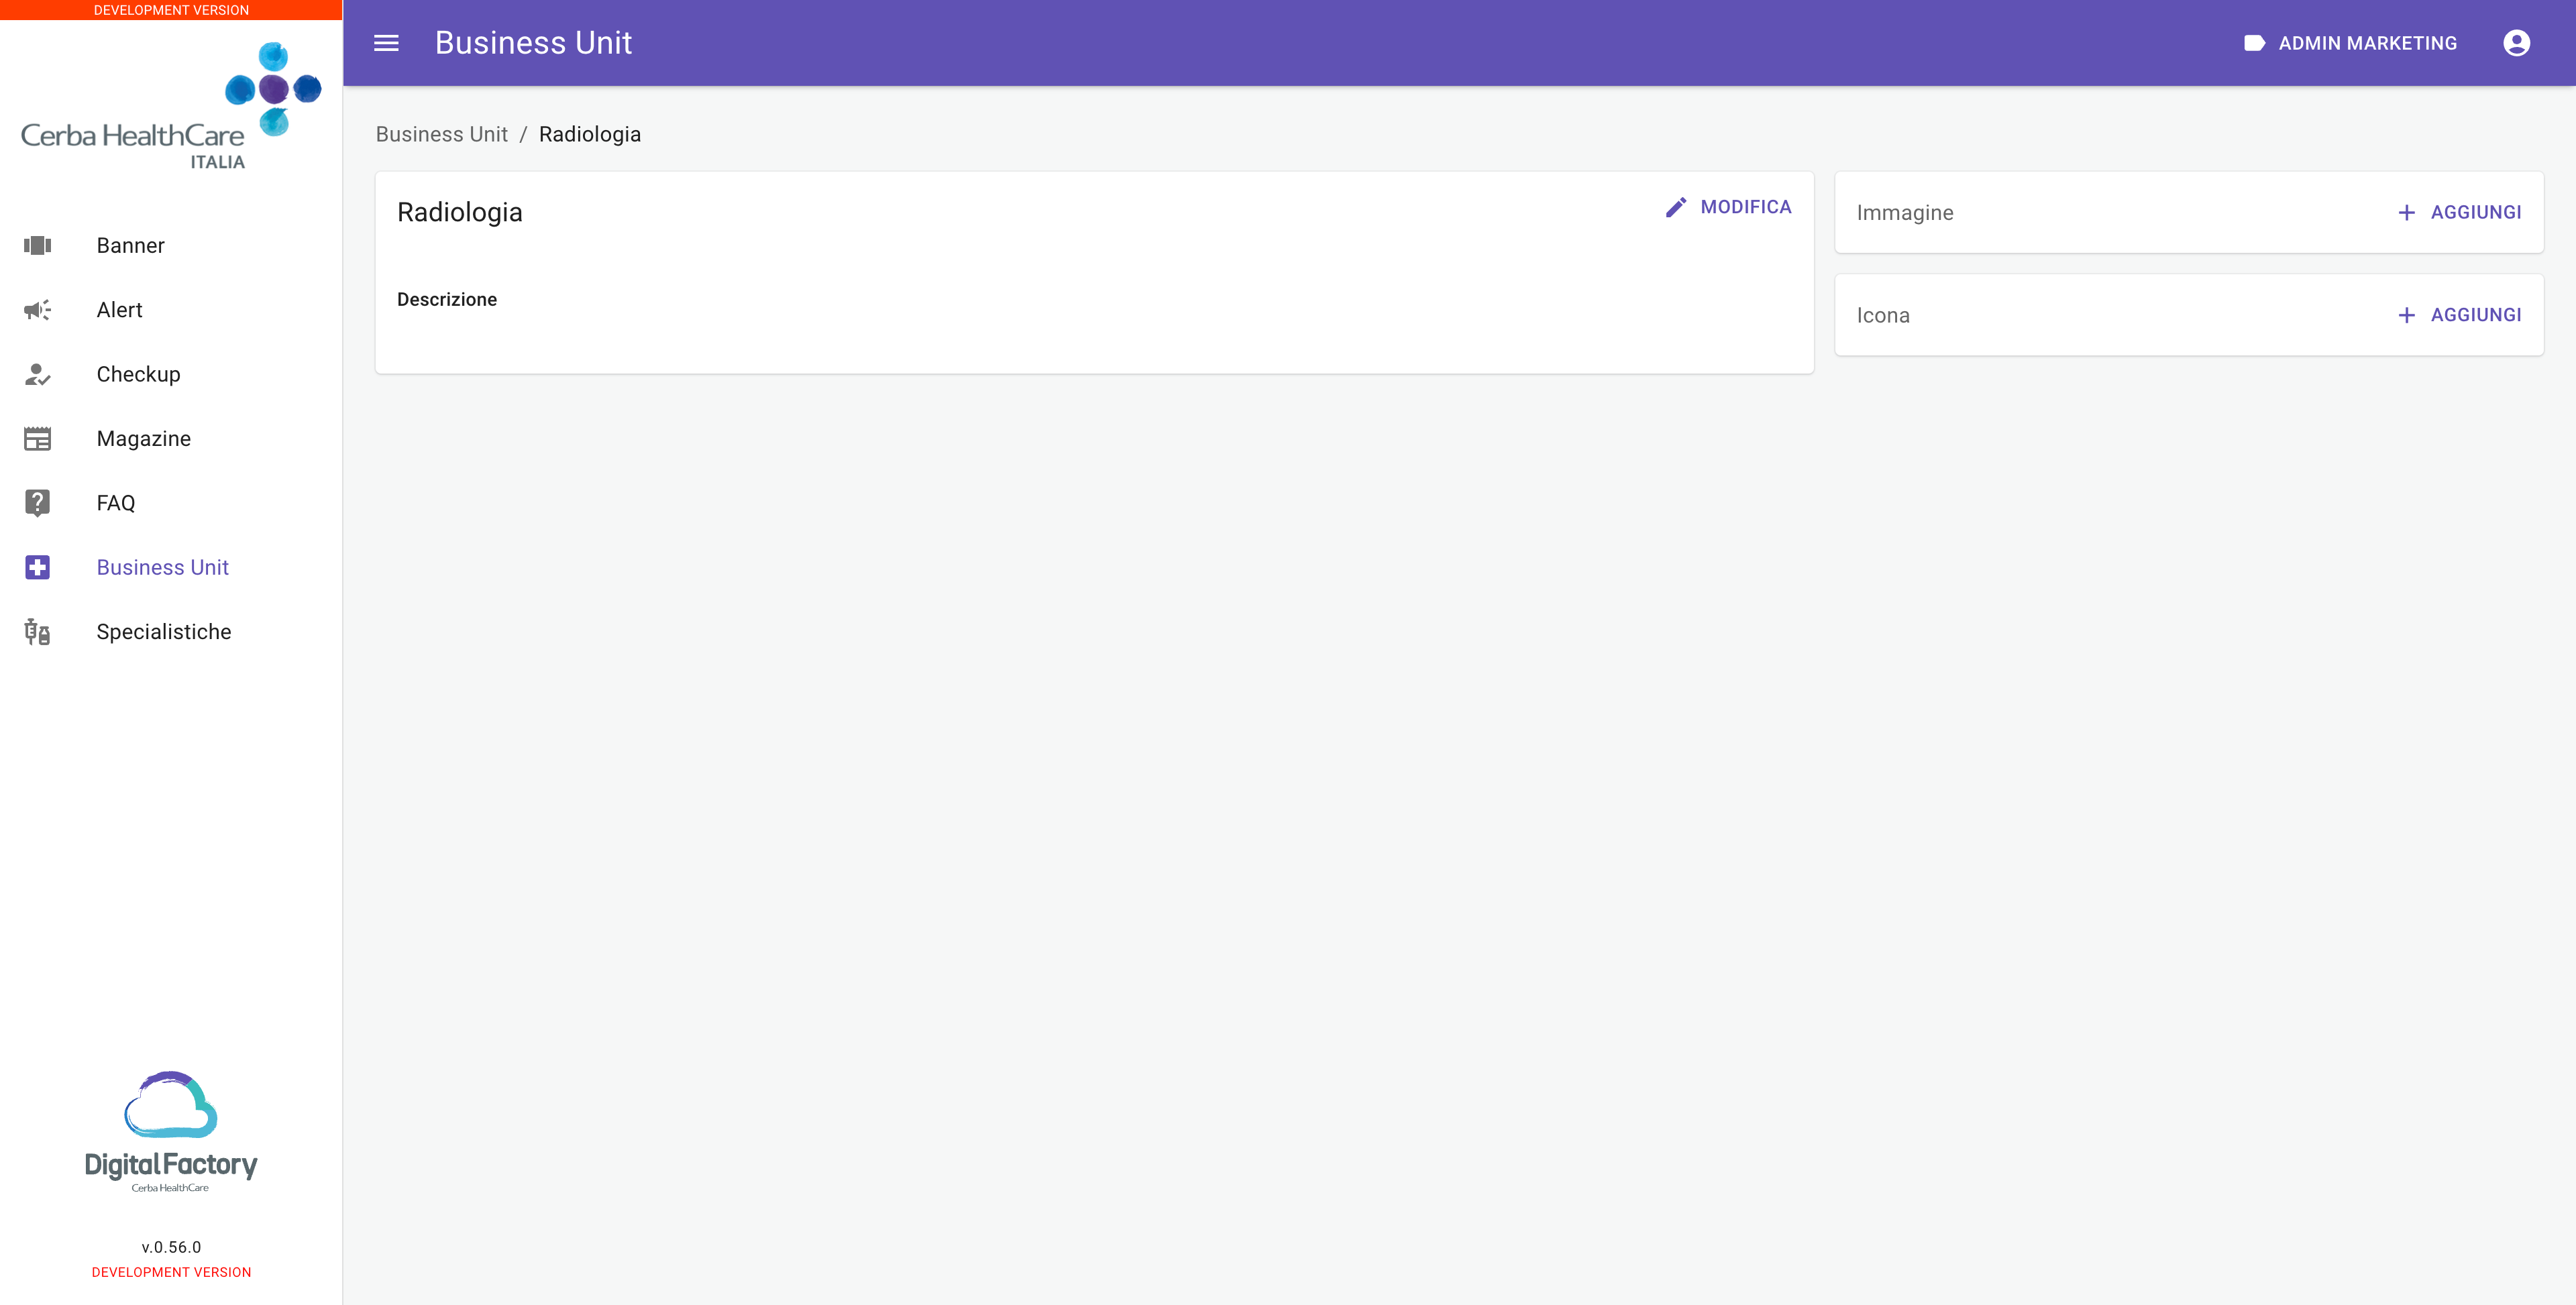
\includegraphics[width=0.75\textwidth]{images/capitolo5/f8_businessUnits/PageBusinessUnit.png} 
    \caption{Pagina dettaglio BU} 
    \label{fig:PageBusinessUnit}
\end{figure}

\begin{figure}[H]
    \centering
    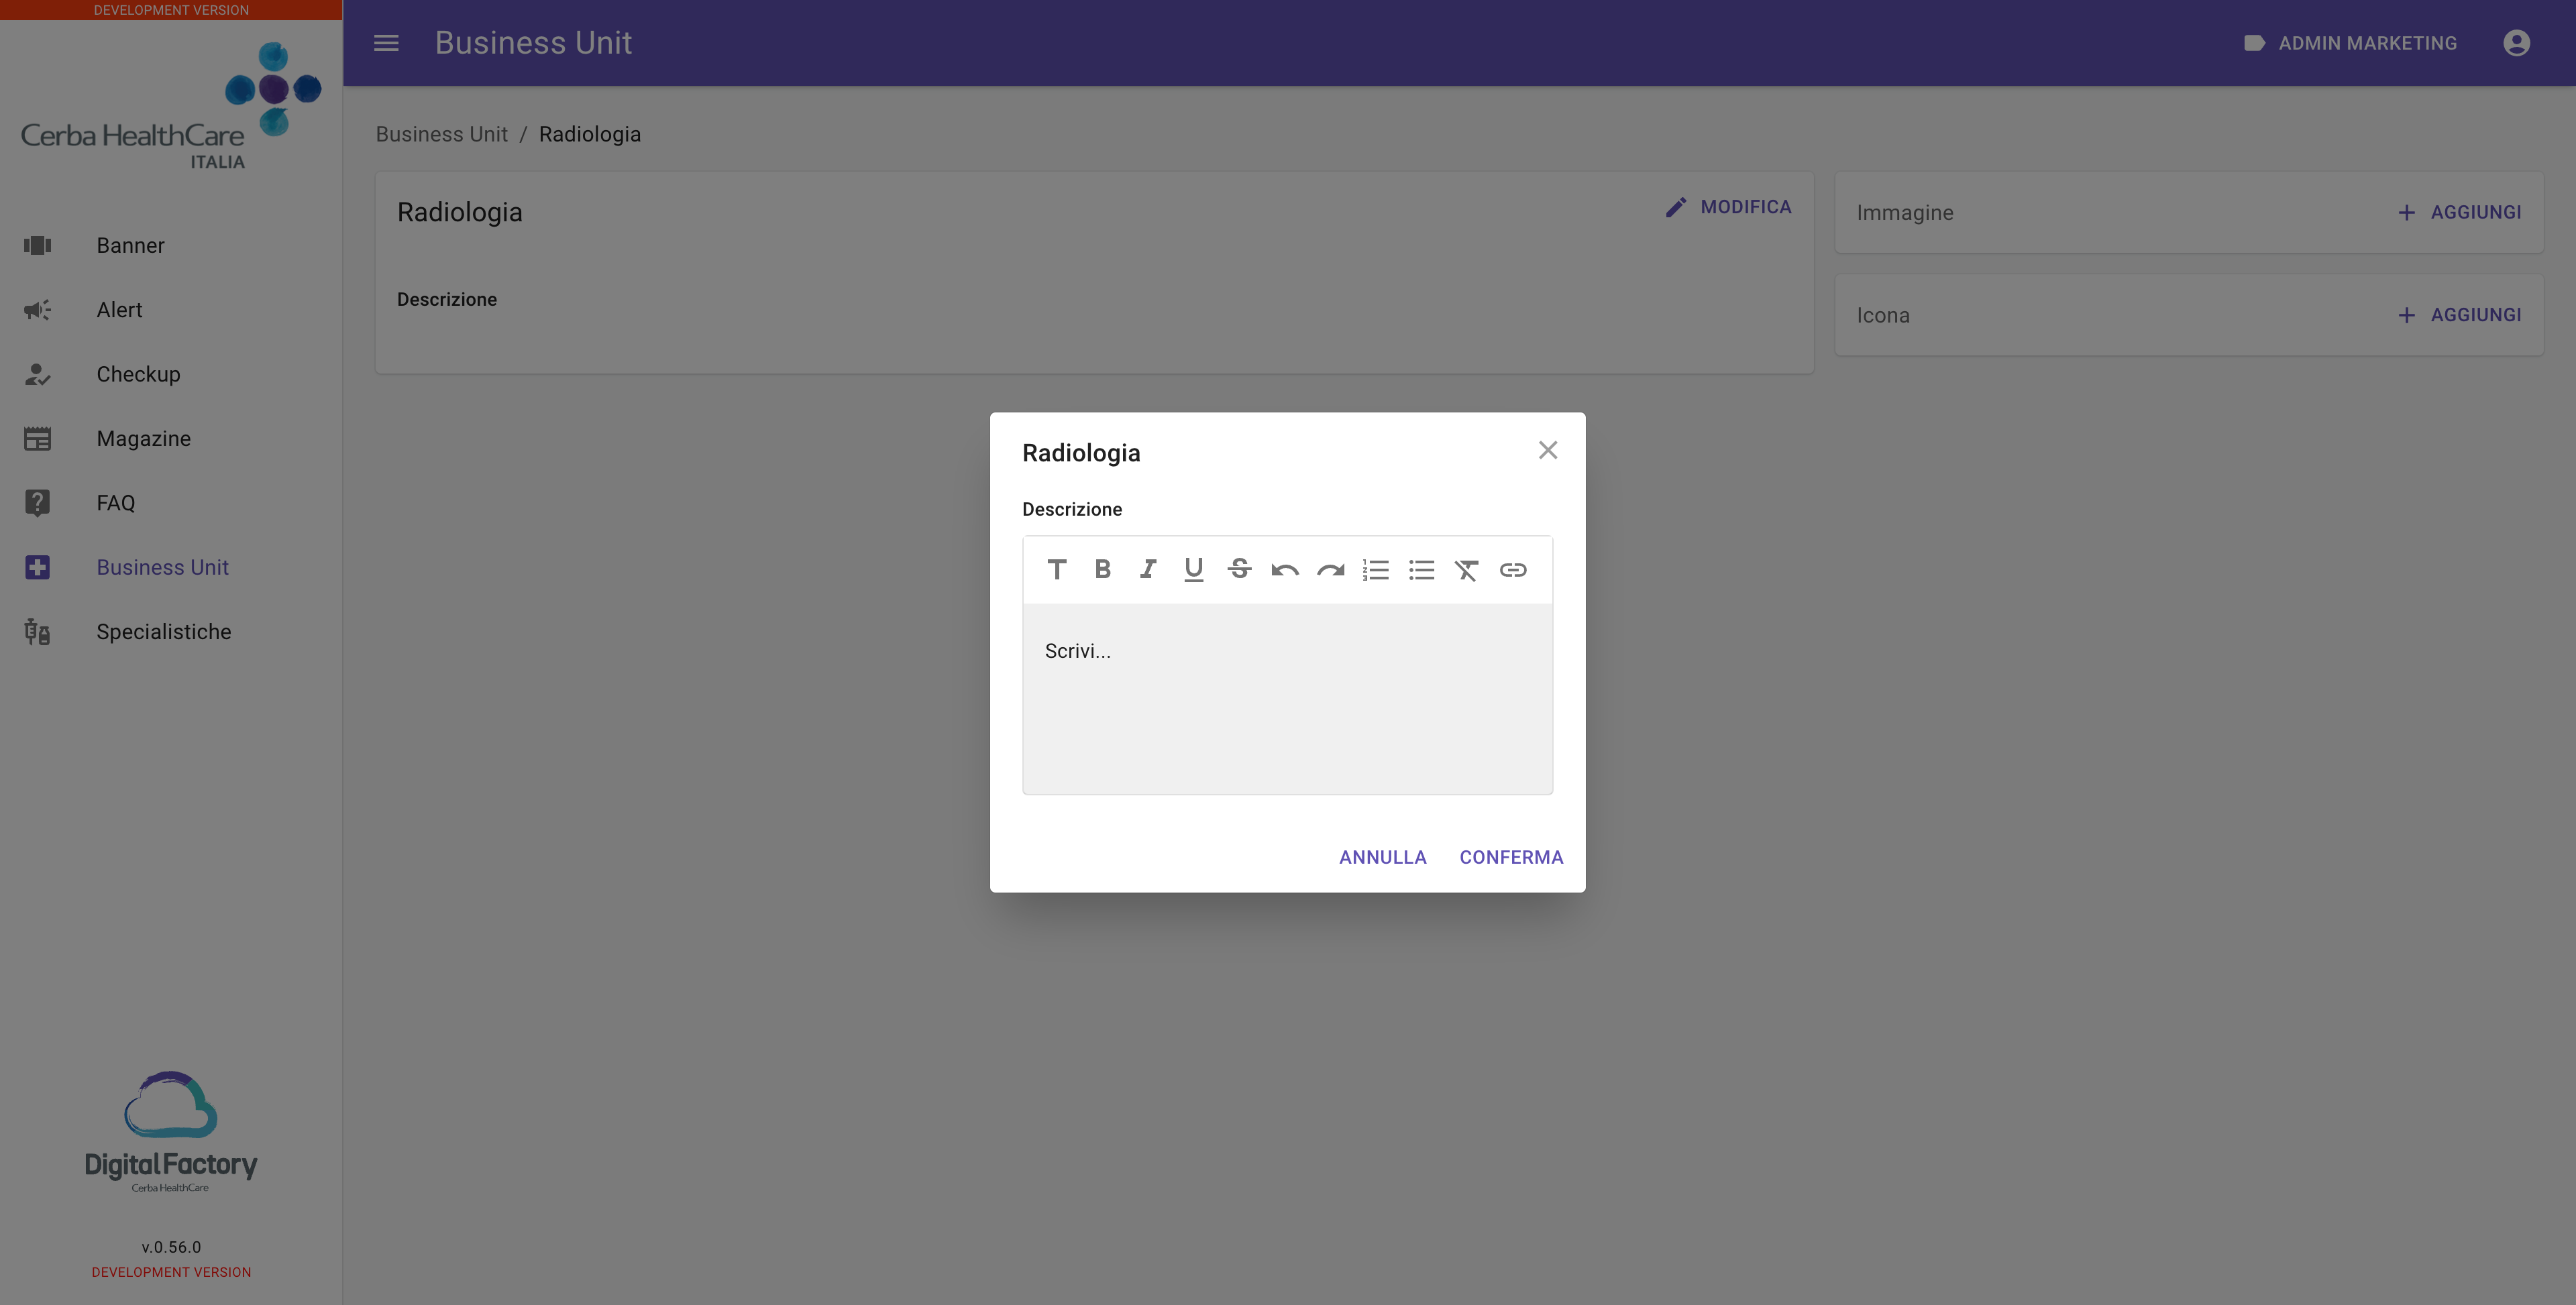
\includegraphics[width=0.75\textwidth]{images/capitolo5/f8_businessUnits/ModalBusinessUnit_edit.png} 
    \caption{Modale modifica descrizione BU} 
    \label{fig:ModalBusinessUnit_edit}
\end{figure}

\begin{figure}[H]
    \centering
    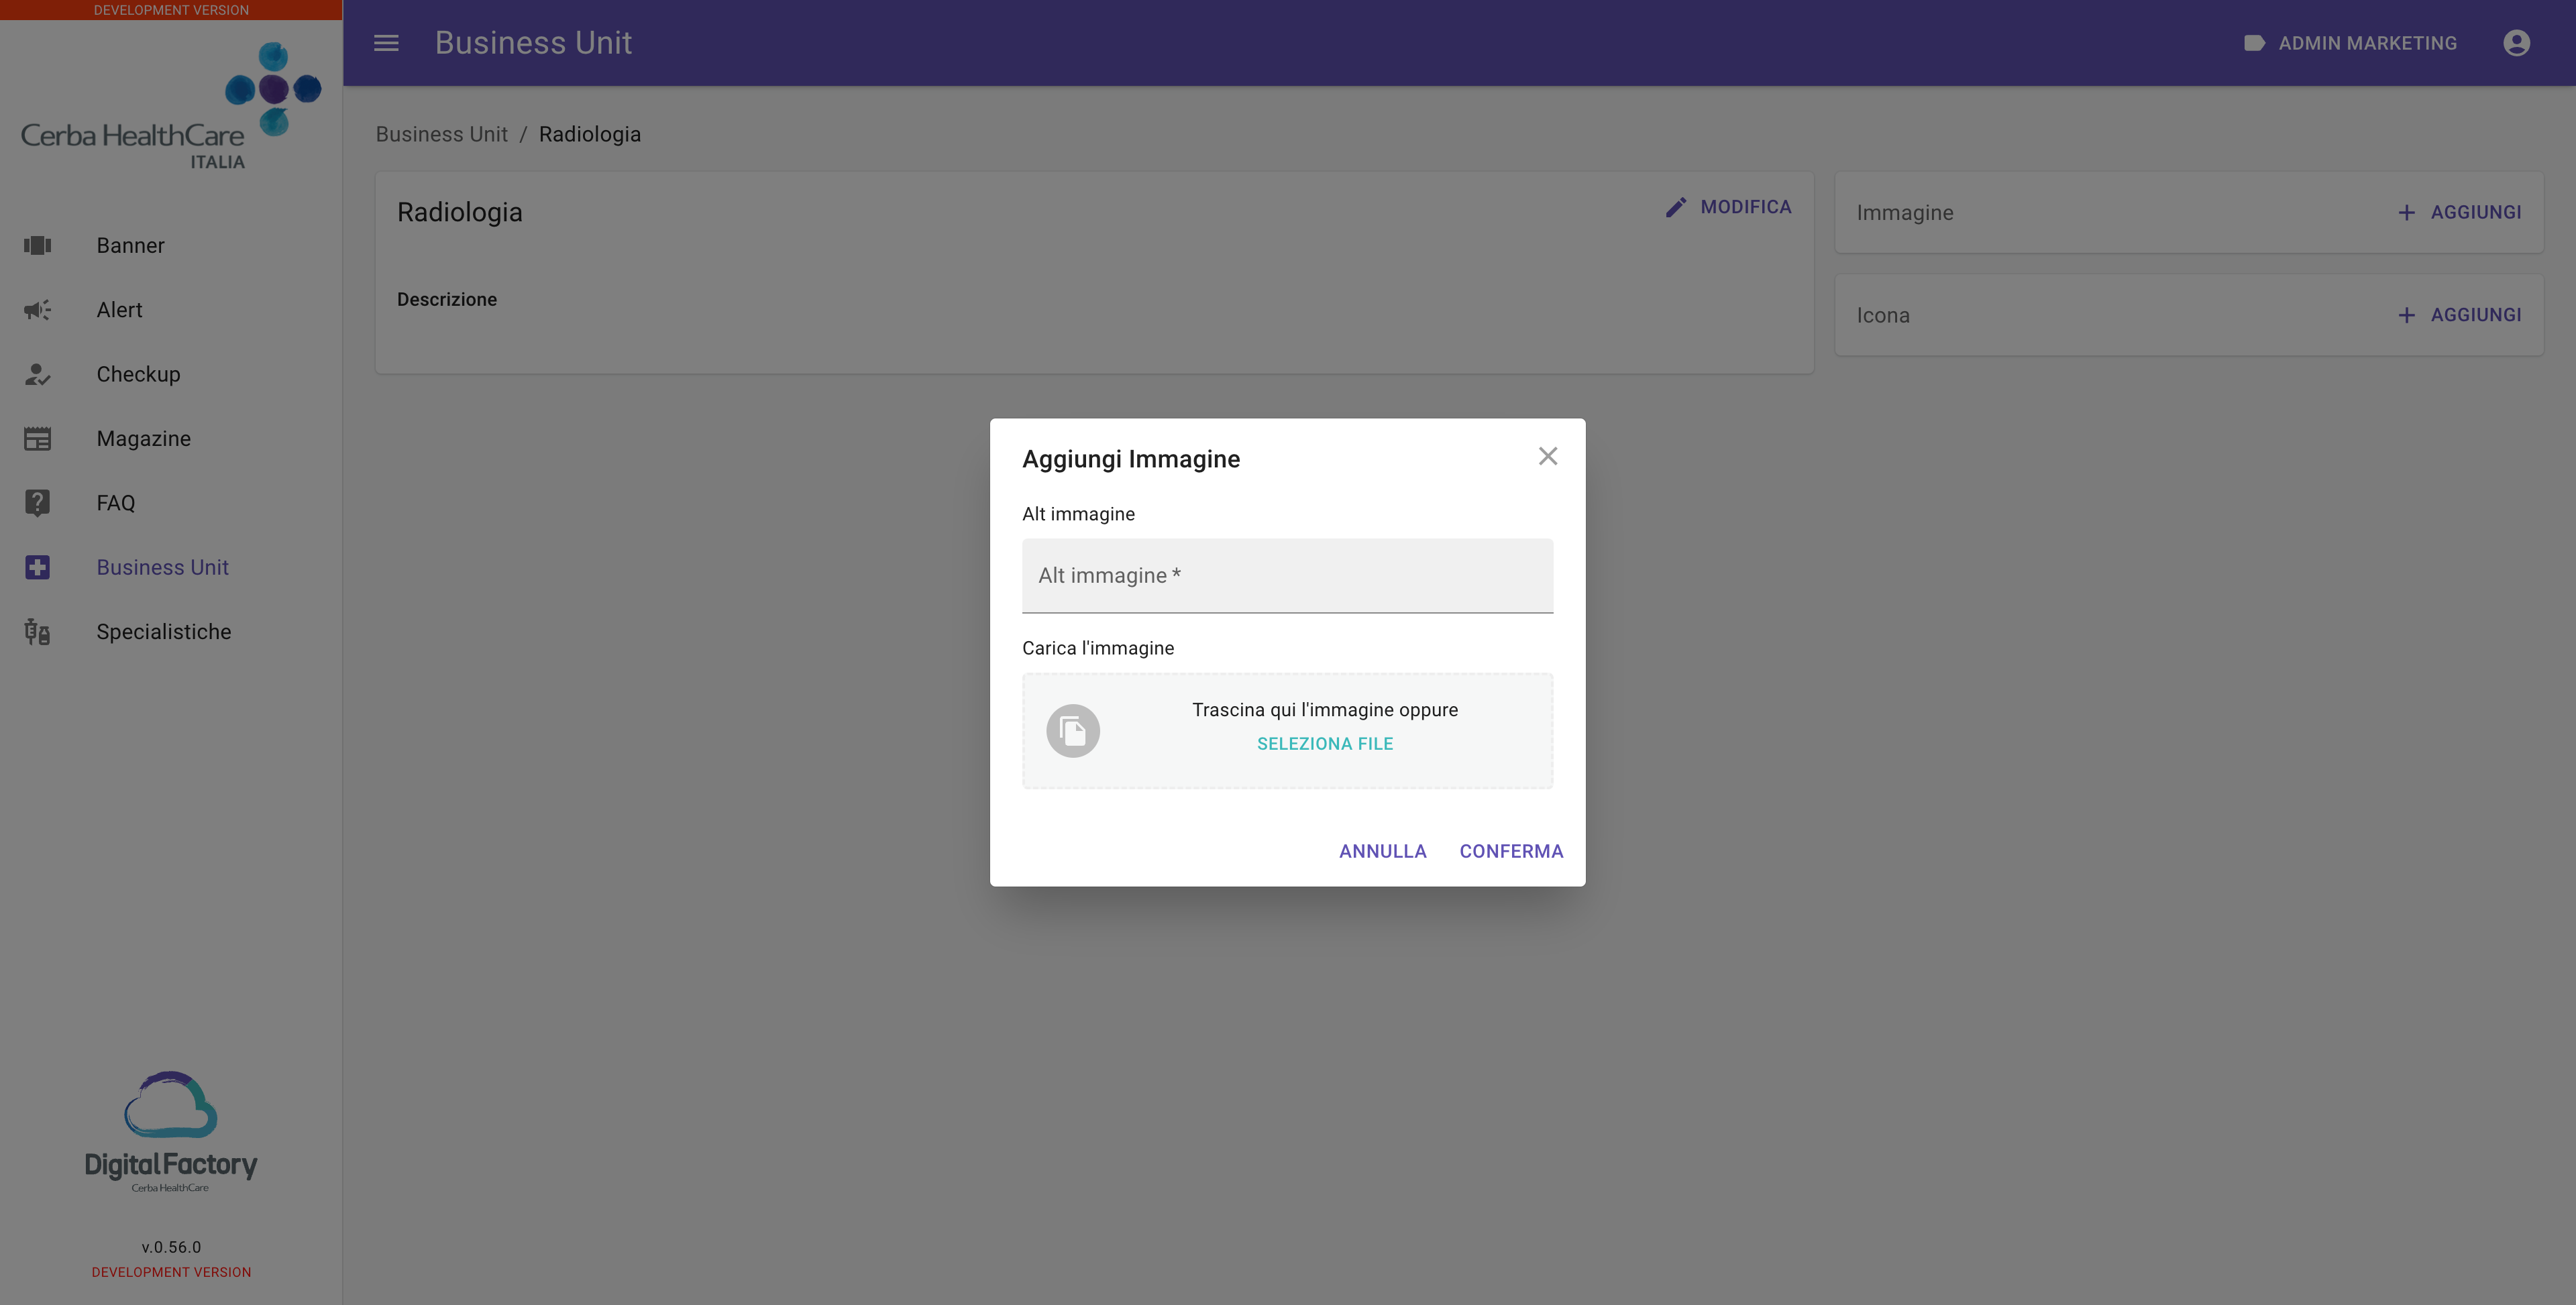
\includegraphics[width=0.75\textwidth]{images/capitolo5/f8_businessUnits/ModalBusinessUnit_createImage.png} 
    \caption{Modale aggiunta immagine BU} 
    \label{fig:ModalBusinessUnit_createImage}
\end{figure}

\begin{figure}[H]
    \centering
    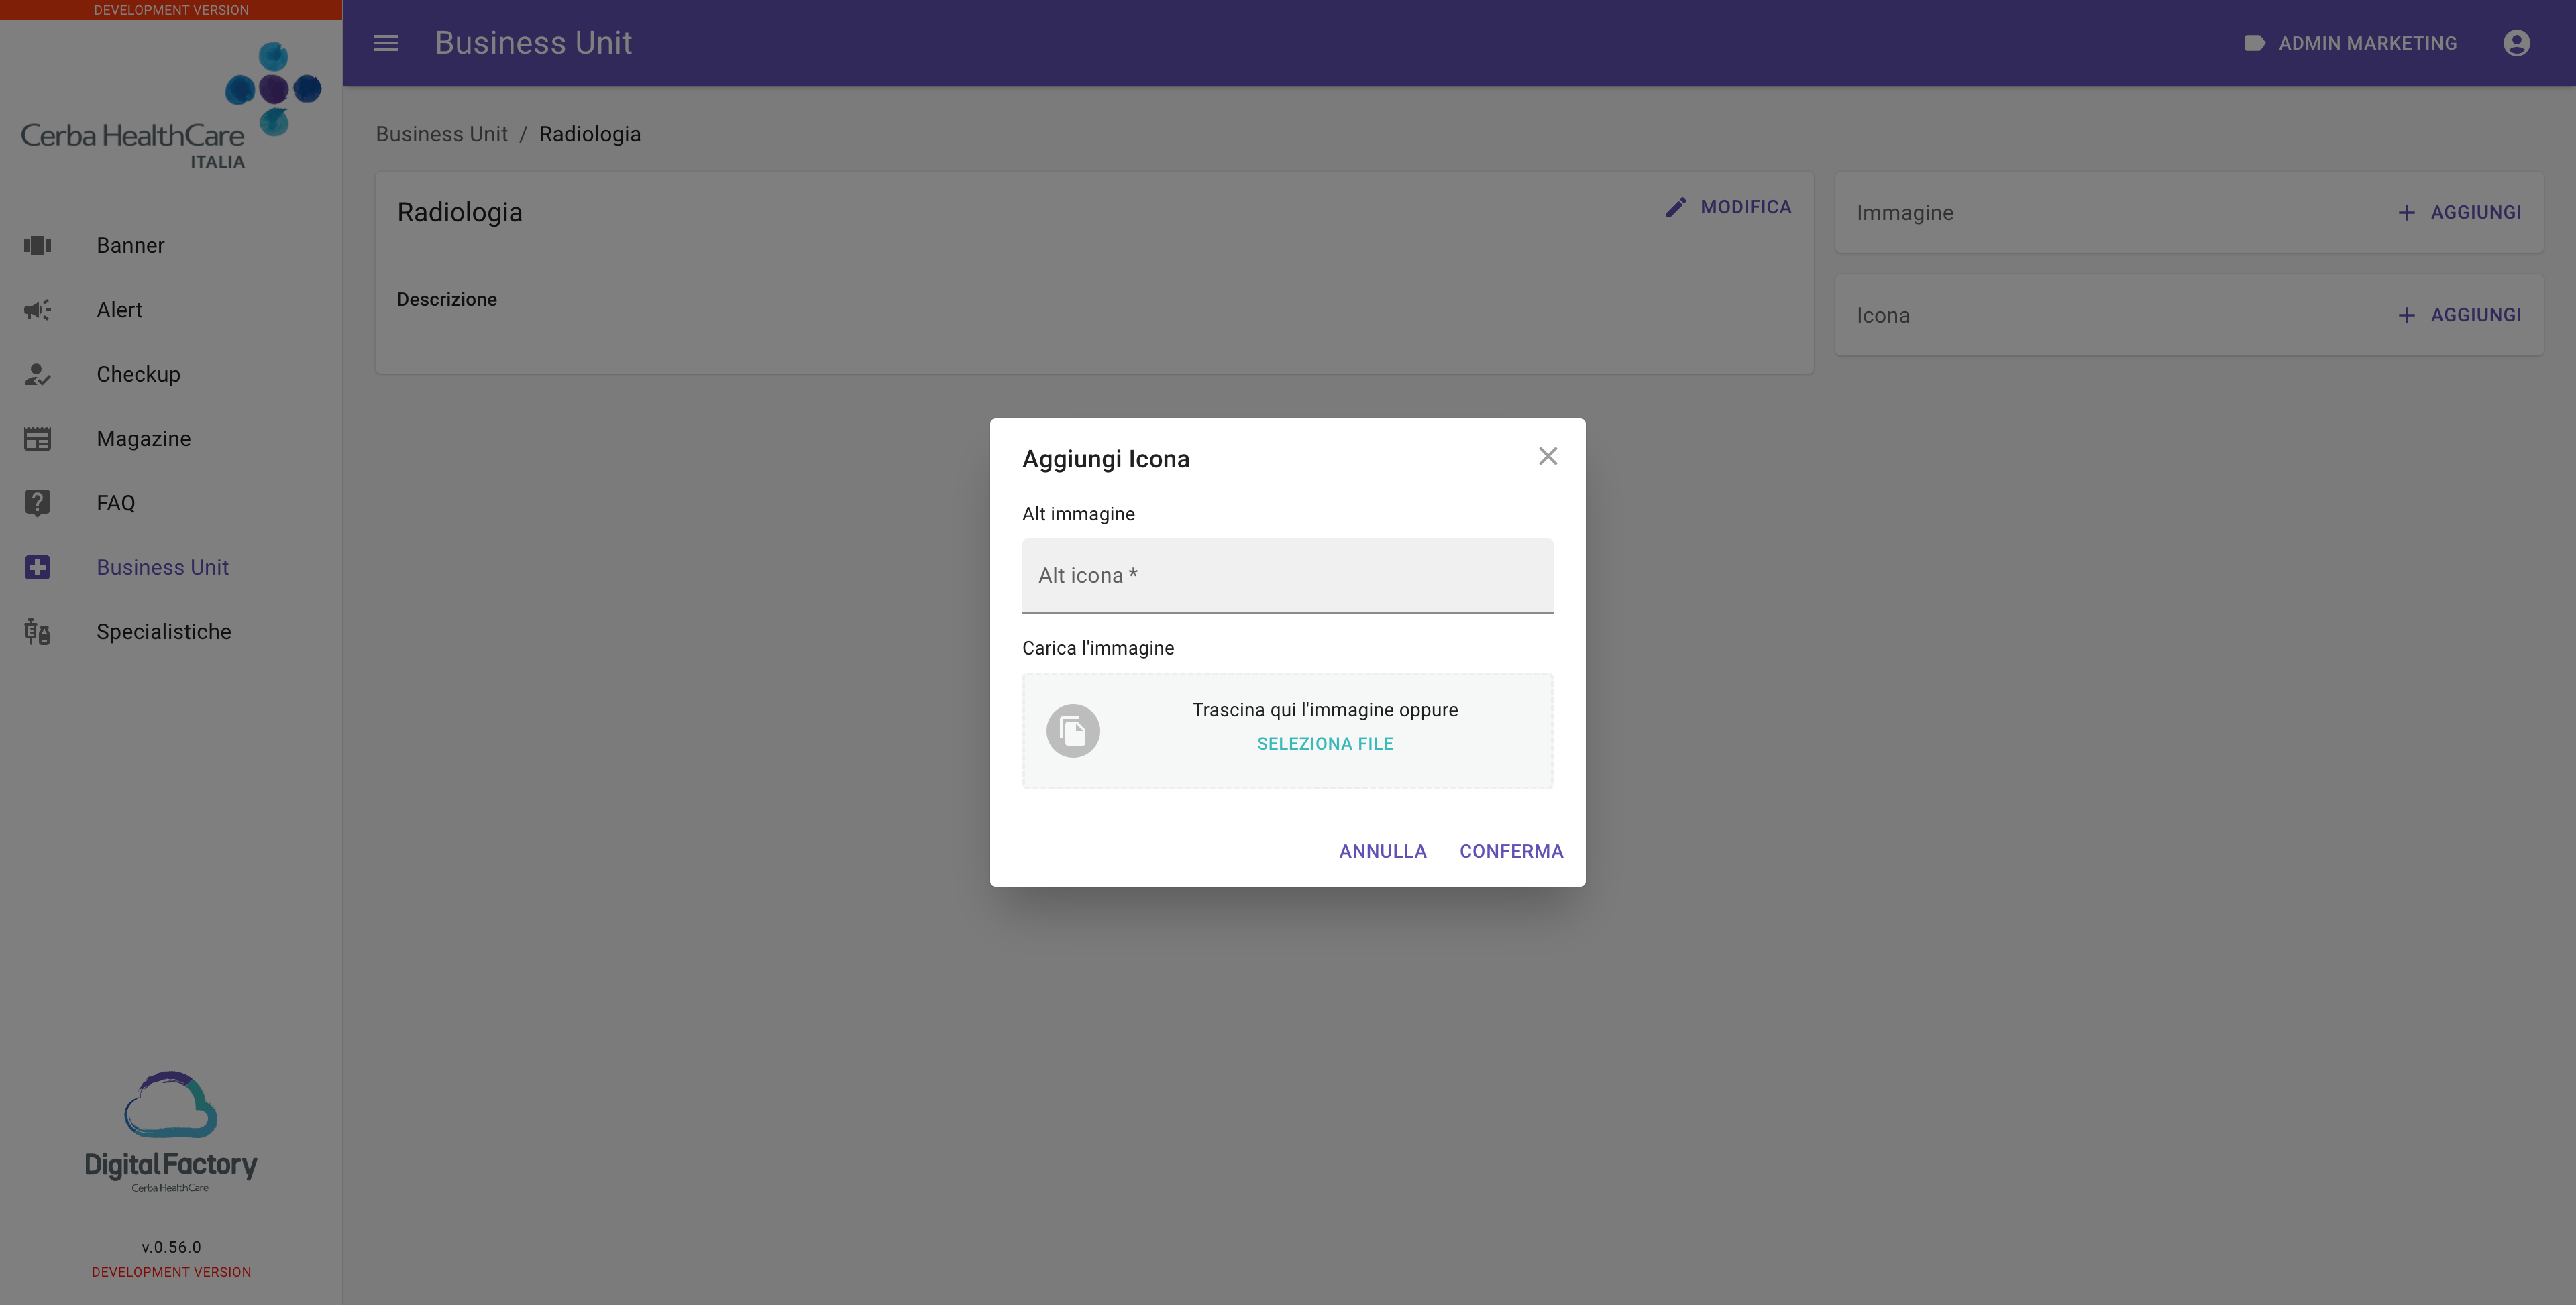
\includegraphics[width=0.75\textwidth]{images/capitolo5/f8_businessUnits/ModalBusinessUnit_createIcon.png} 
    \caption{Modale aggiunta icona BU} 
    \label{fig:ModalBusinessUnit_createIcon}
\end{figure}

\begin{figure}[H]
    \centering
    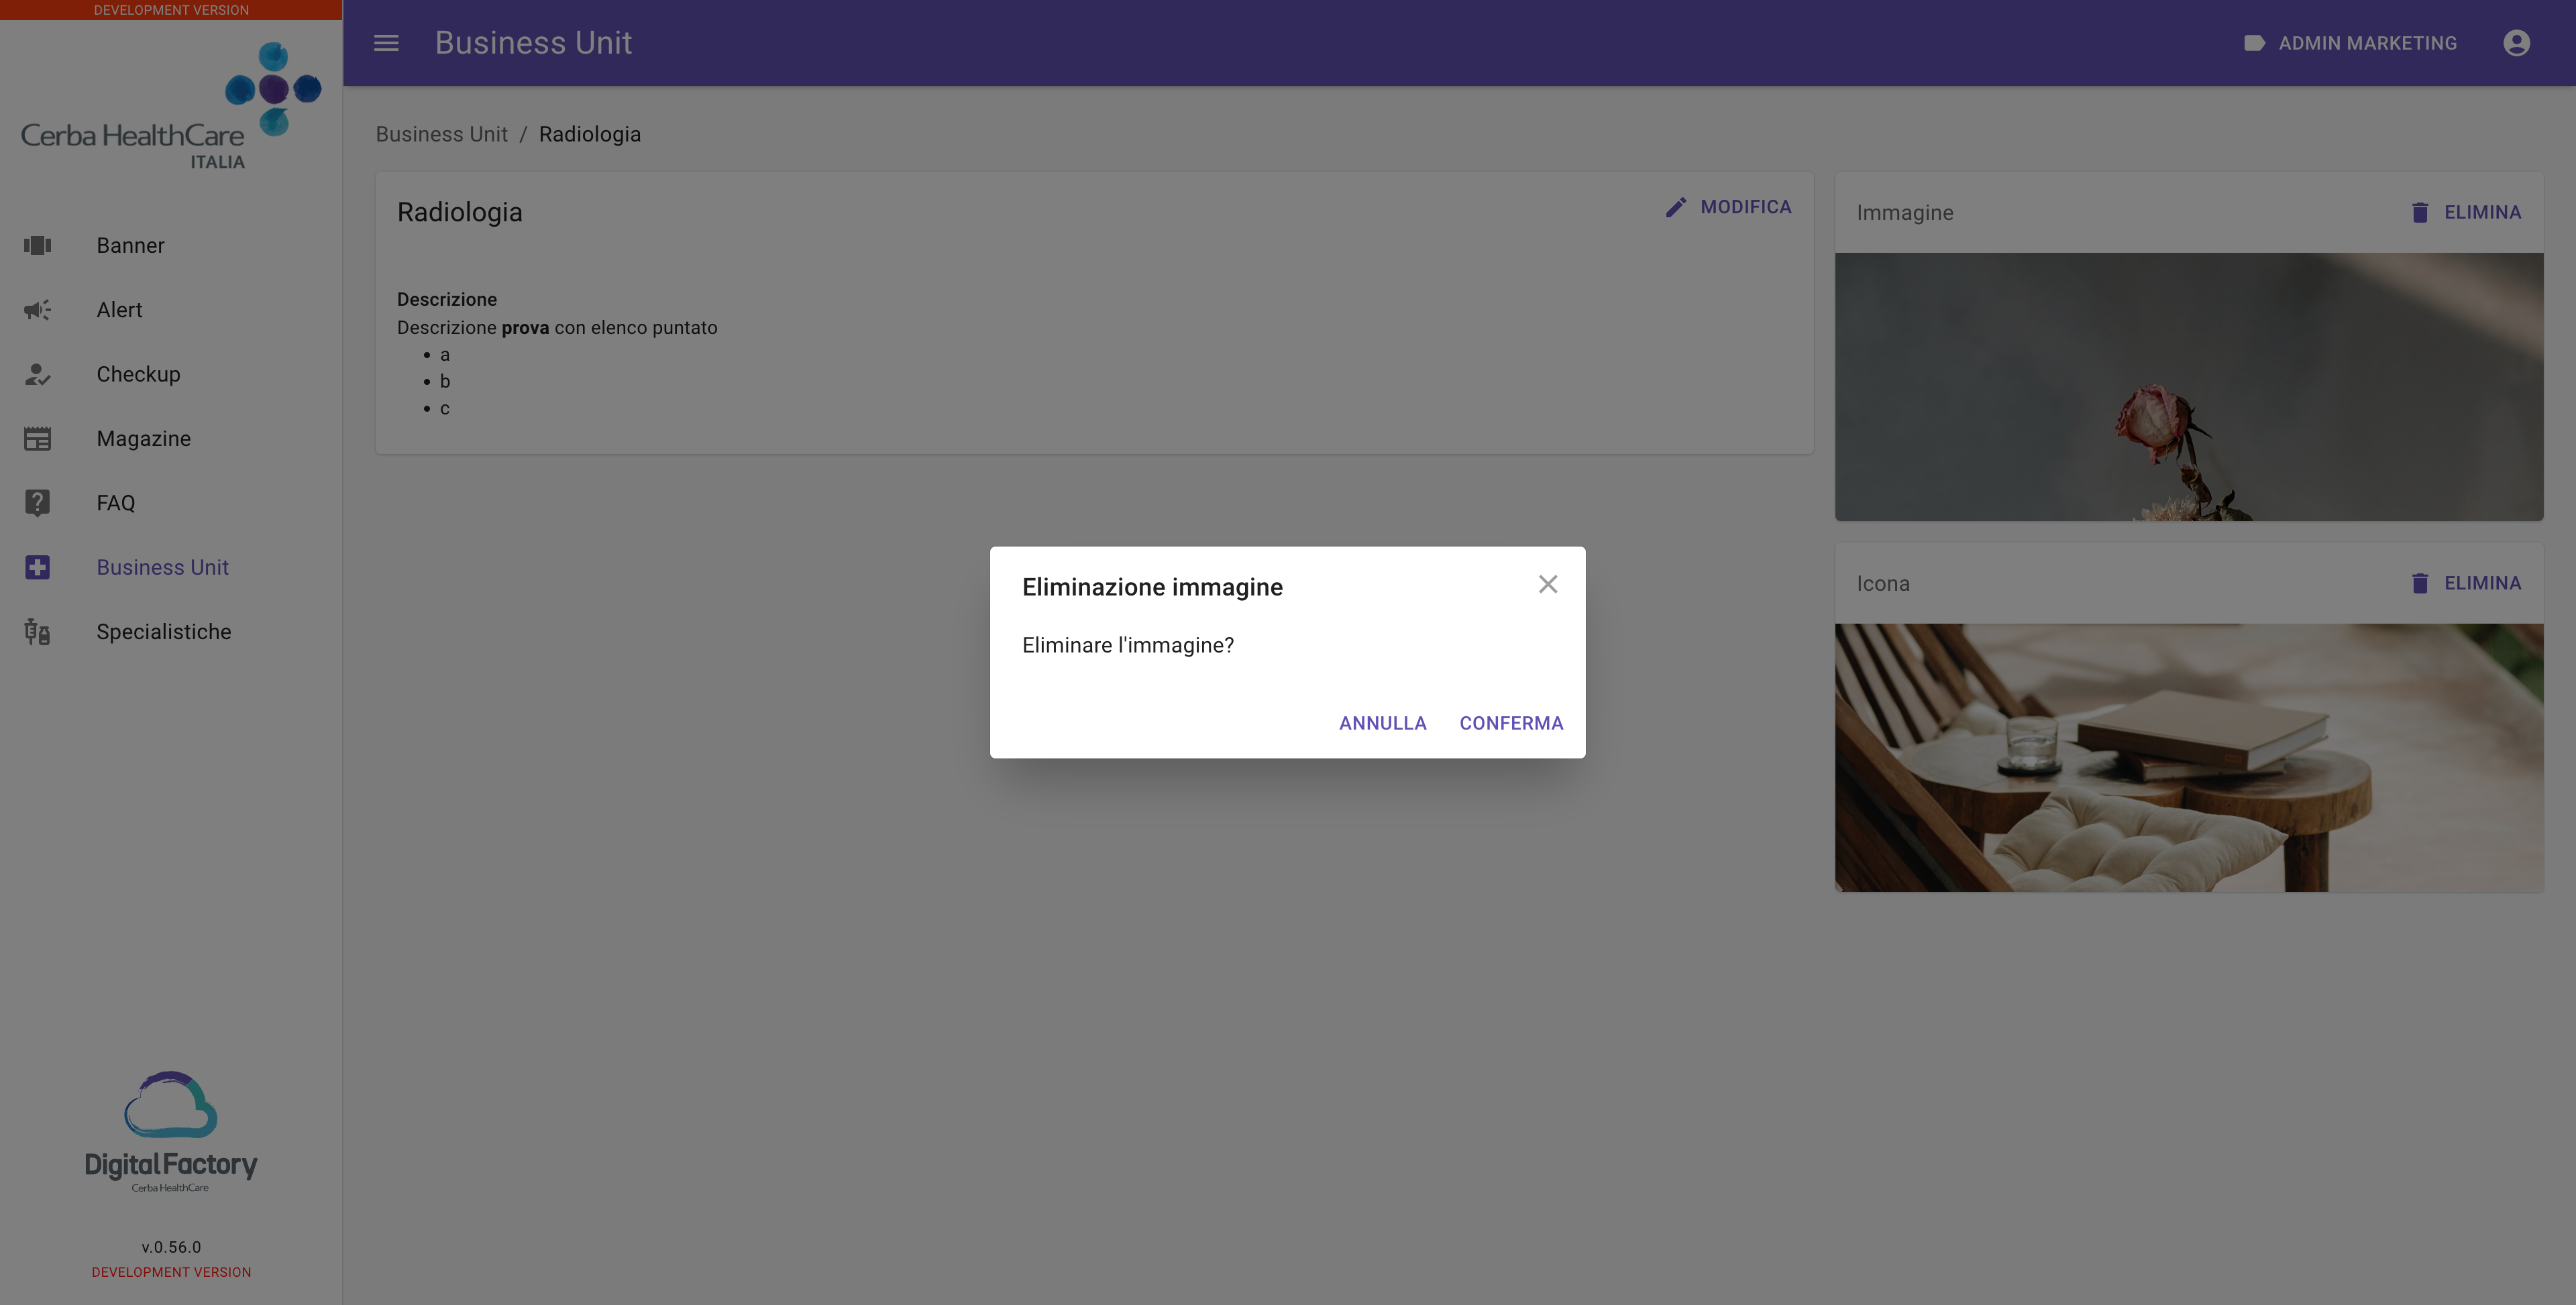
\includegraphics[width=0.75\textwidth]{images/capitolo5/f8_businessUnits/ModalBusinessUnit_deleteImage.png} 
    \caption{Modale eliminazione immagine BU} 
    \label{fig:ModalBusinessUnit_deleteImage}
\end{figure}

\begin{figure}[H]
    \centering
    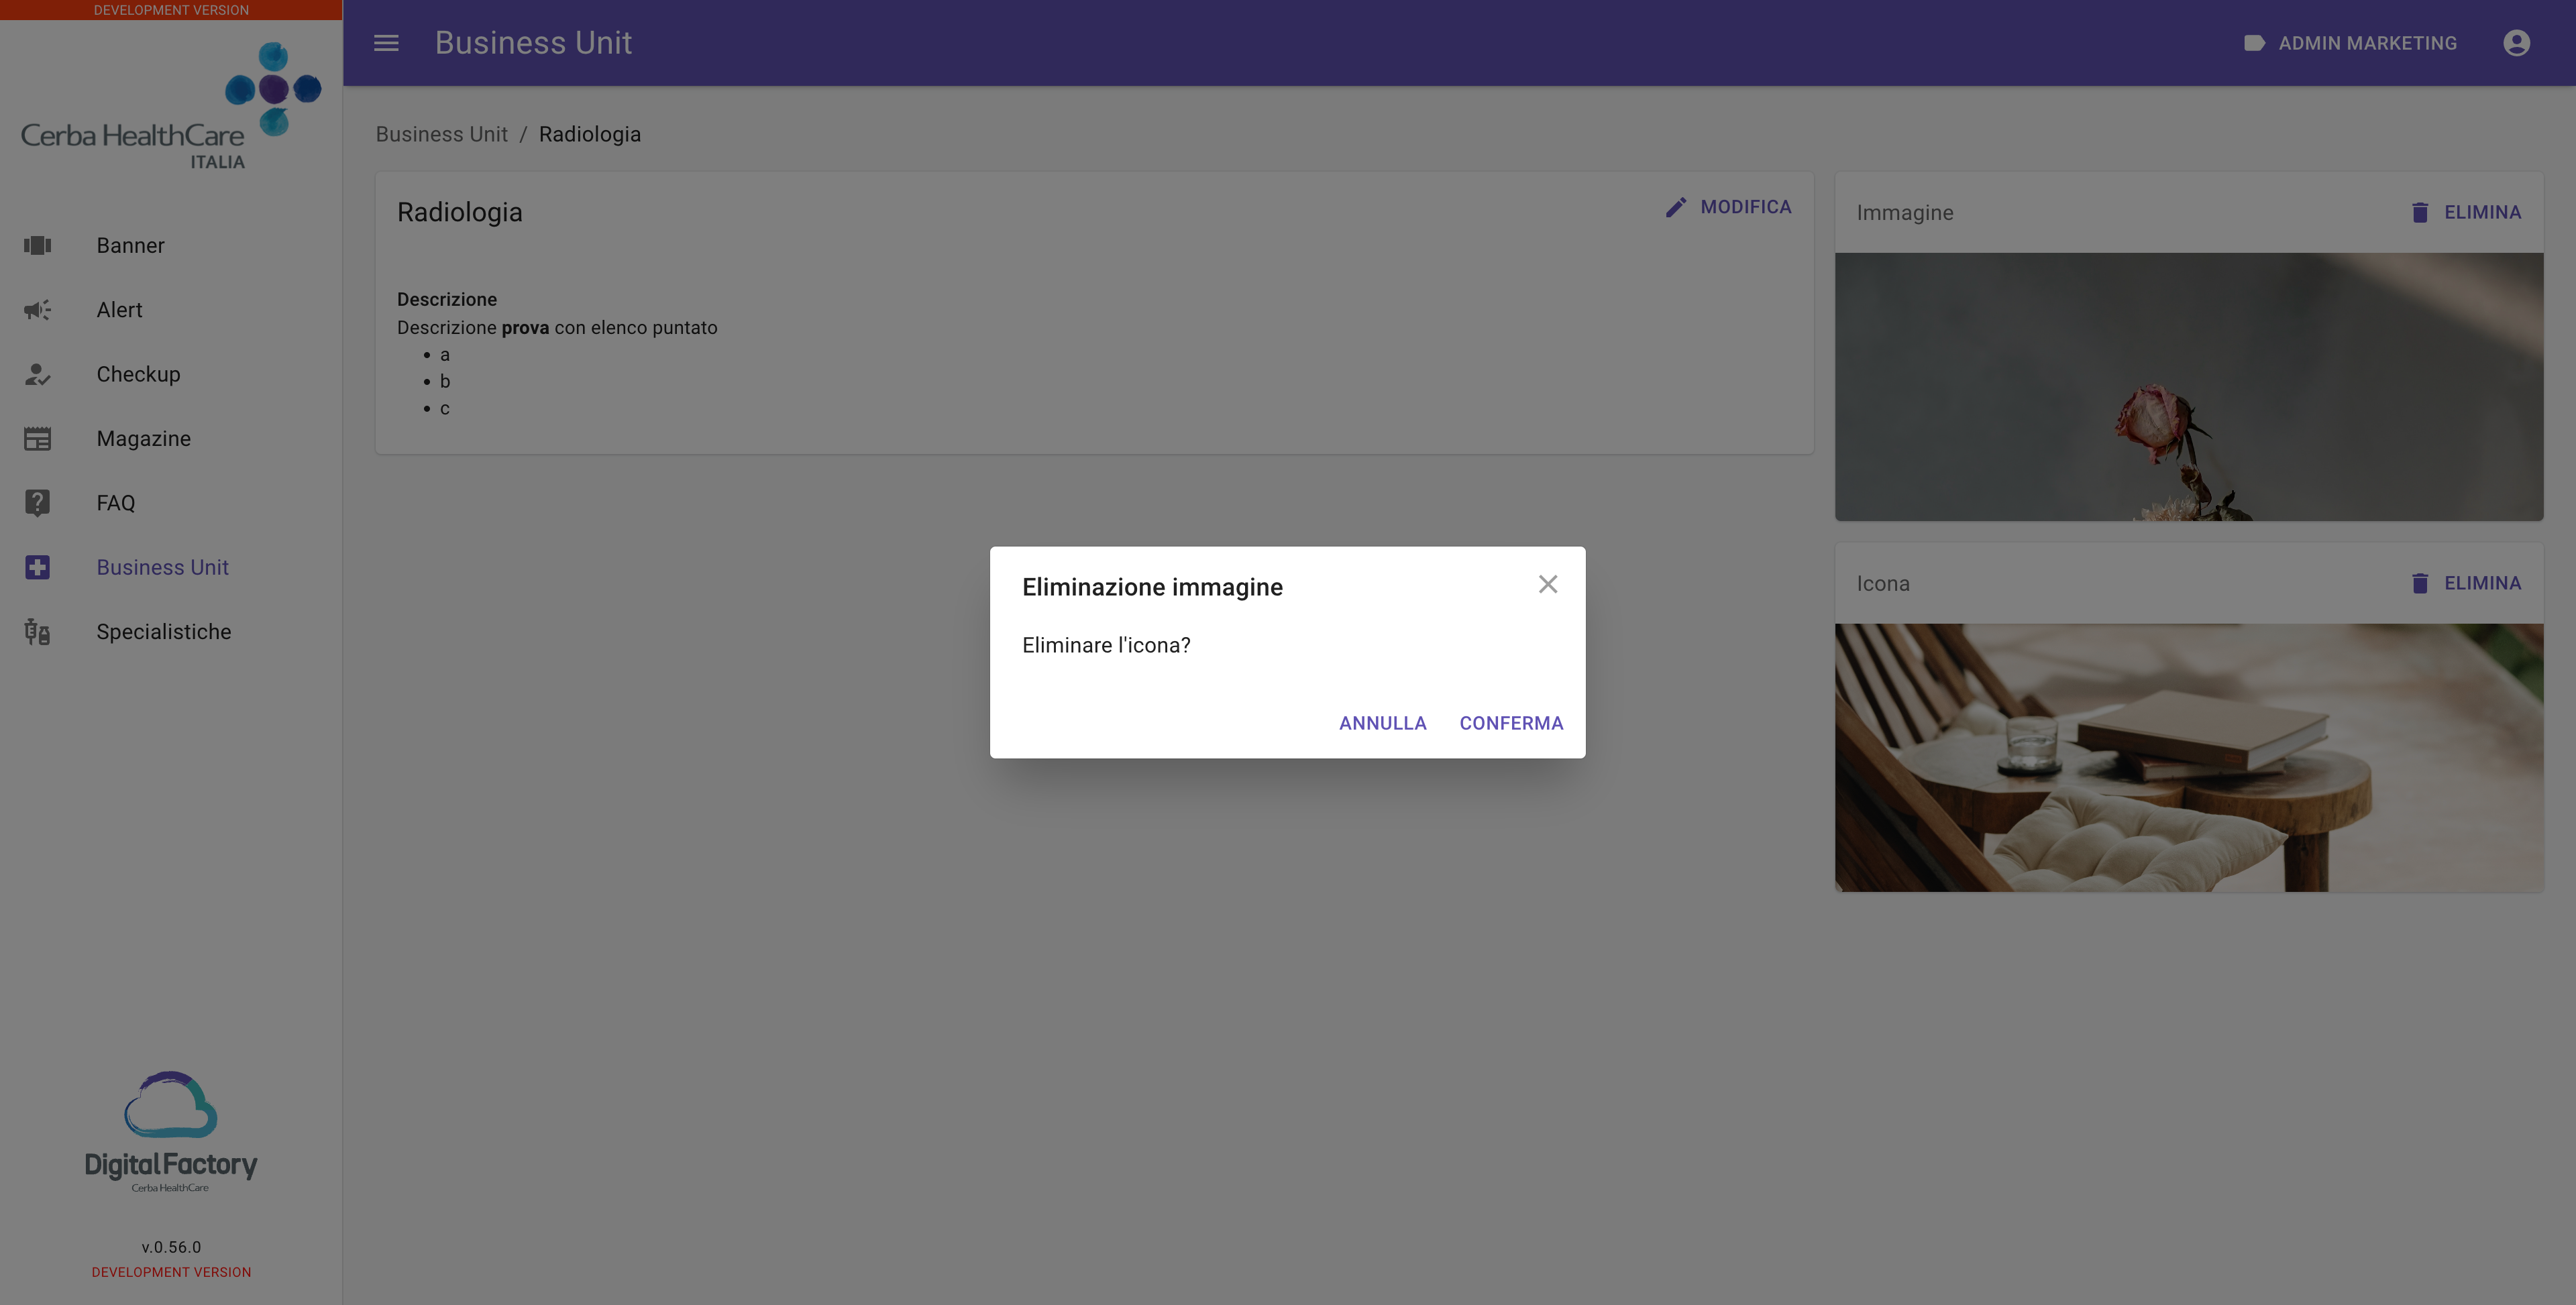
\includegraphics[width=0.75\textwidth]{images/capitolo5/f8_businessUnits/ModalBusinessUnit_deleteIcon.png} 
    \caption{Modale eliminazione icona BU} 
    \label{fig:ModalBusinessUnit_deleteIcon}
\end{figure}

\subsection{F9: “Specialistiche”}
\subparagraph{Requisiti}
Aggiungere la sezione “Specialistiche” fra quelle previste per il ruolo utente \textit{marketing admin}.\\
Al suo interno, una tabella deve mostrare le specialistiche esistenti in una lista semplice e riportarne la proprietà “Nome”.\\
L'\textit{header} della tabella delle specialistiche deve essere dotato di un campo di ricerca. Questo deve essere in grado di filtrare per nome e posizionato all'estrema destra dell'\textit{header} della tabella.\\
Ogni specialistica deve essere dotata di una pagina di dettaglio alla quale si accede cliccando sul link posto in concomitanza del nome. Qui, deve essere possibile modificare e visualizzare la descrizione, proprietà che deve poter essere formattata; sempre all'interno della pagina di dettaglio, si devono poter aggiungere, visualizzare ed eliminare un'immagine e un'icona.

\subsection{F10: “Posizoni aperte”}
\subparagraph{Requisiti}
Aggiungere la sezione “Posizioni aperte” fra quelle previste per il ruolo utente \textit{hr admin}.\\
Al suo interno, una tabella deve mostrare le posizioni aperte esistenti in una lista semplice e riportarne la proprietà “Città”, “Data”, “Area” e “Nome”.\\
Deve essere possibile aggiungere o eliminare una posizione.\\
L'\textit{header} della tabella delle posizioni aperte deve essere dotato di un campo di ricerca. Questo deve essere in grado di filtrare per nome e posizionato posizionato alla sinistra del bottone per l'aggiunta di una nuova posizione.\\
Ogni posizione aperta deve essere dotata di una pagina di dettaglio alla quale si accede cliccando sul link posto in concomitanza del nome. Qui, deve essere possibile modificare e visualizzare i campi delle informazioni, e solamente per la proprietà “Descrizione” deve essere fornita la possibilità di formattazione.

\paragraph{\textit{Output} grafico}
\begin{figure}[H]
    \centering
    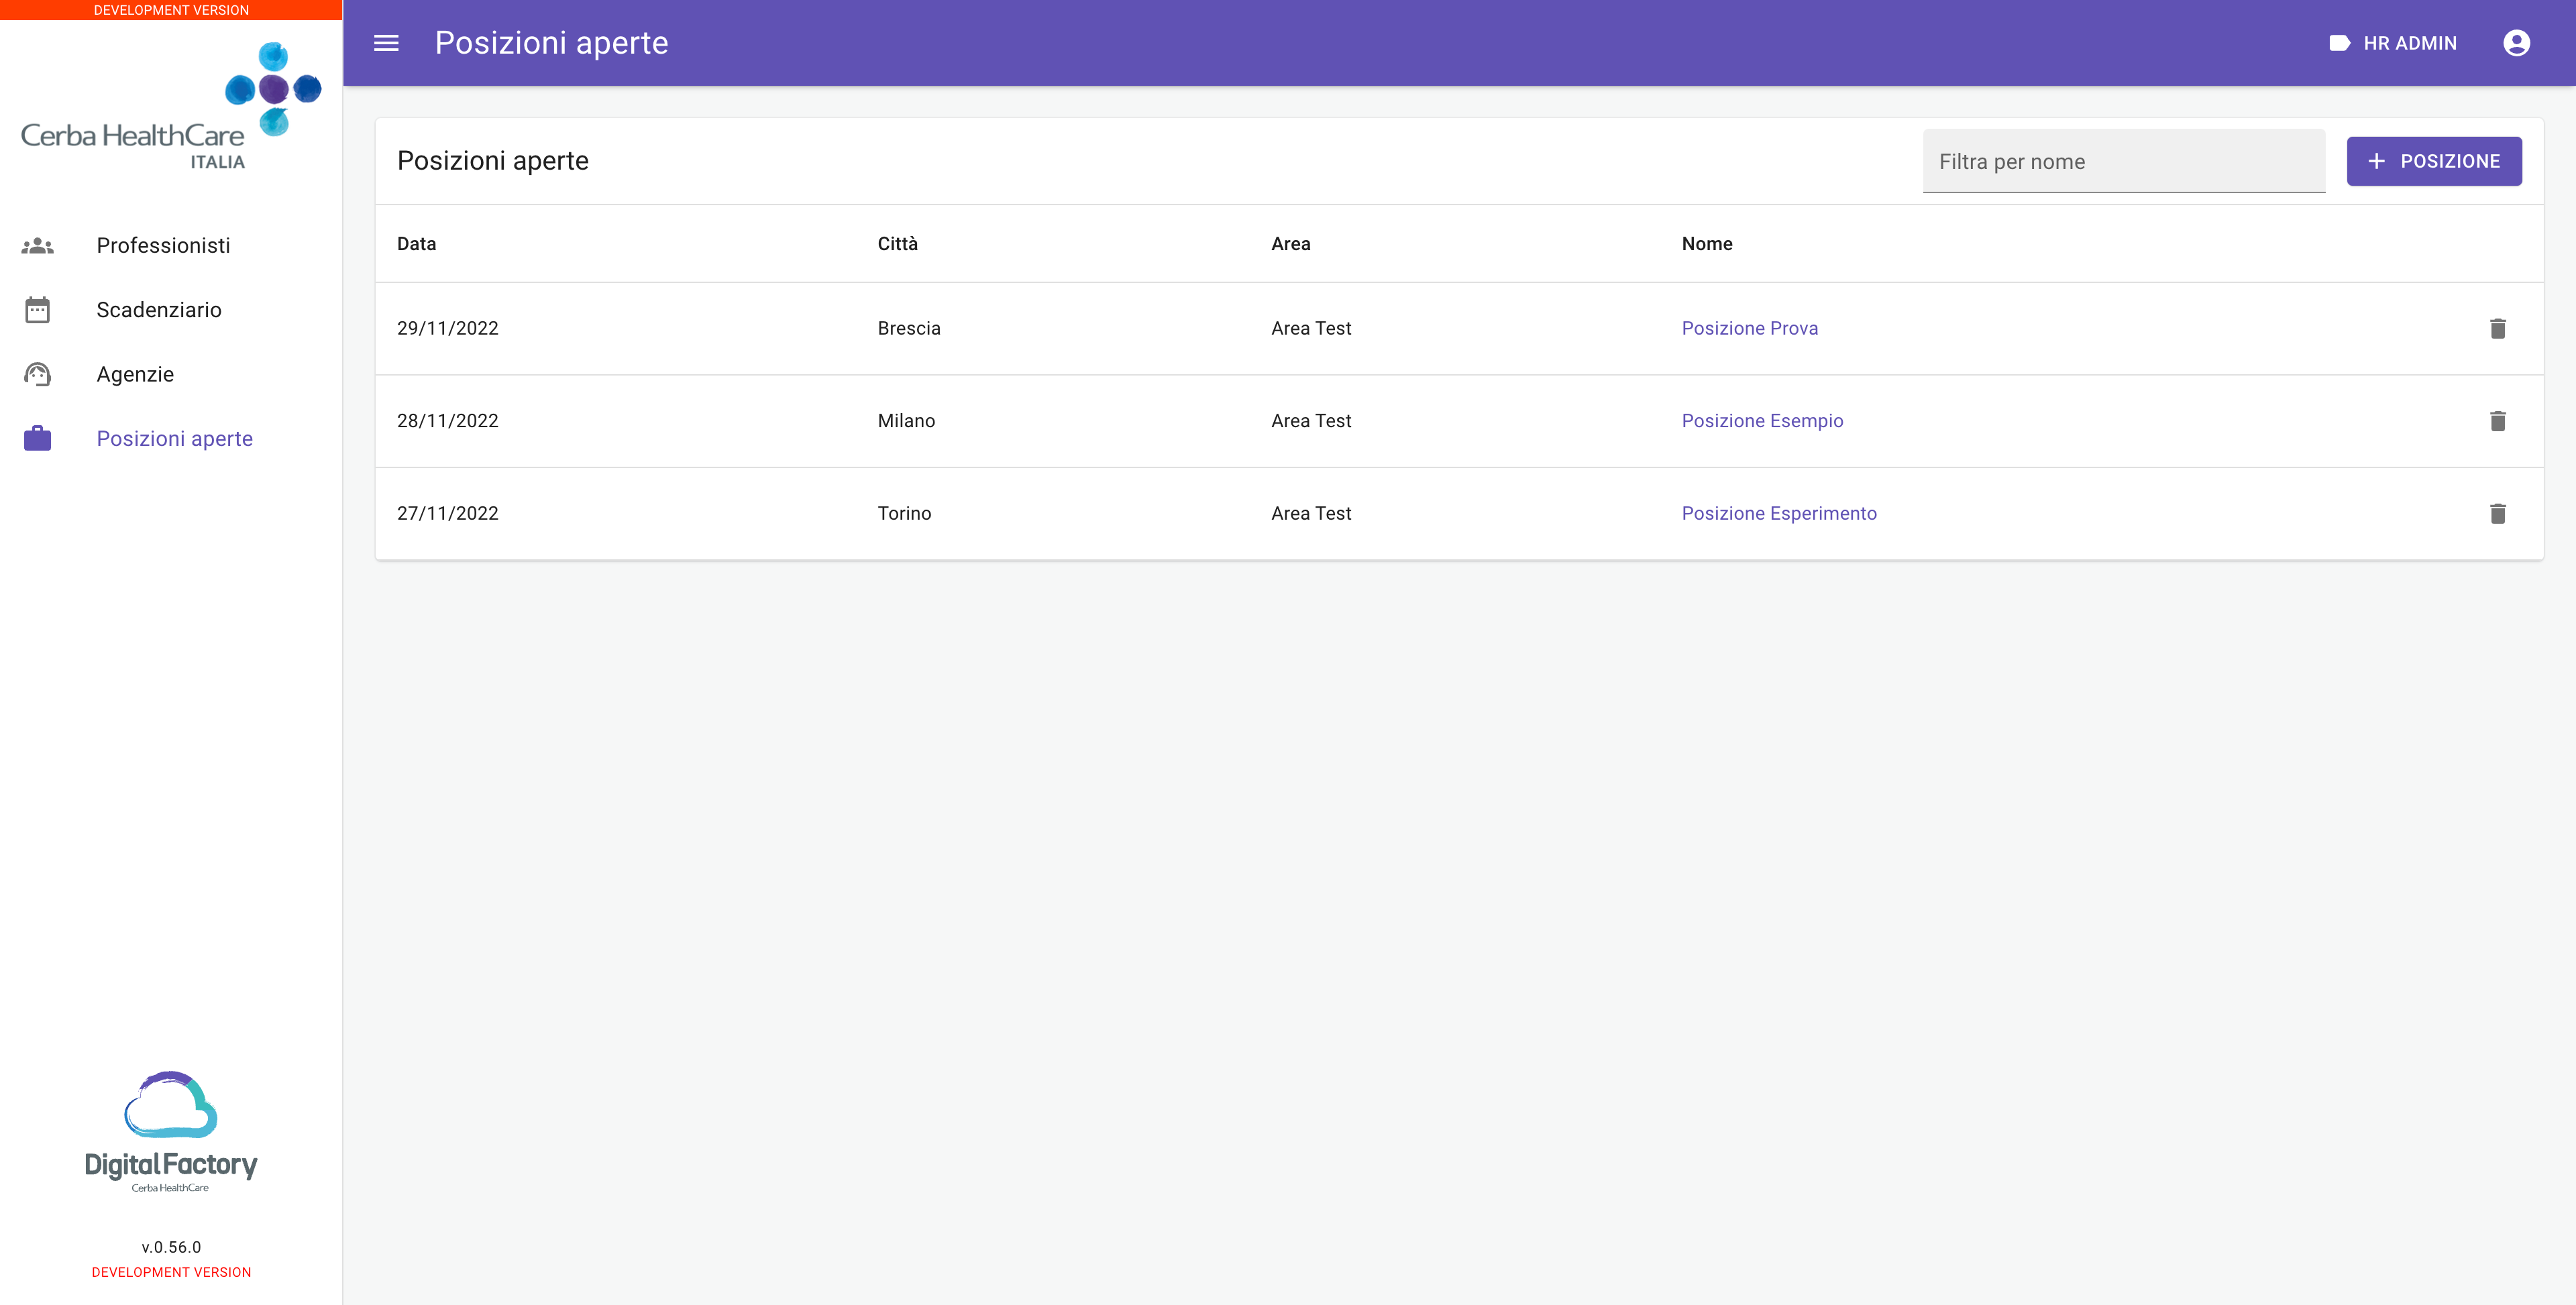
\includegraphics[width=0.75\textwidth]{images/capitolo5/f10_jobOpenPositions/PageJobOpenPositions_searchEmpty.png} 
    \caption{Tabella posizioni aperte campo ricerca vuoto} 
    \label{fig:PageJobOpenPositions_searchEmpty}
\end{figure}

\begin{figure}[H]
    \centering
    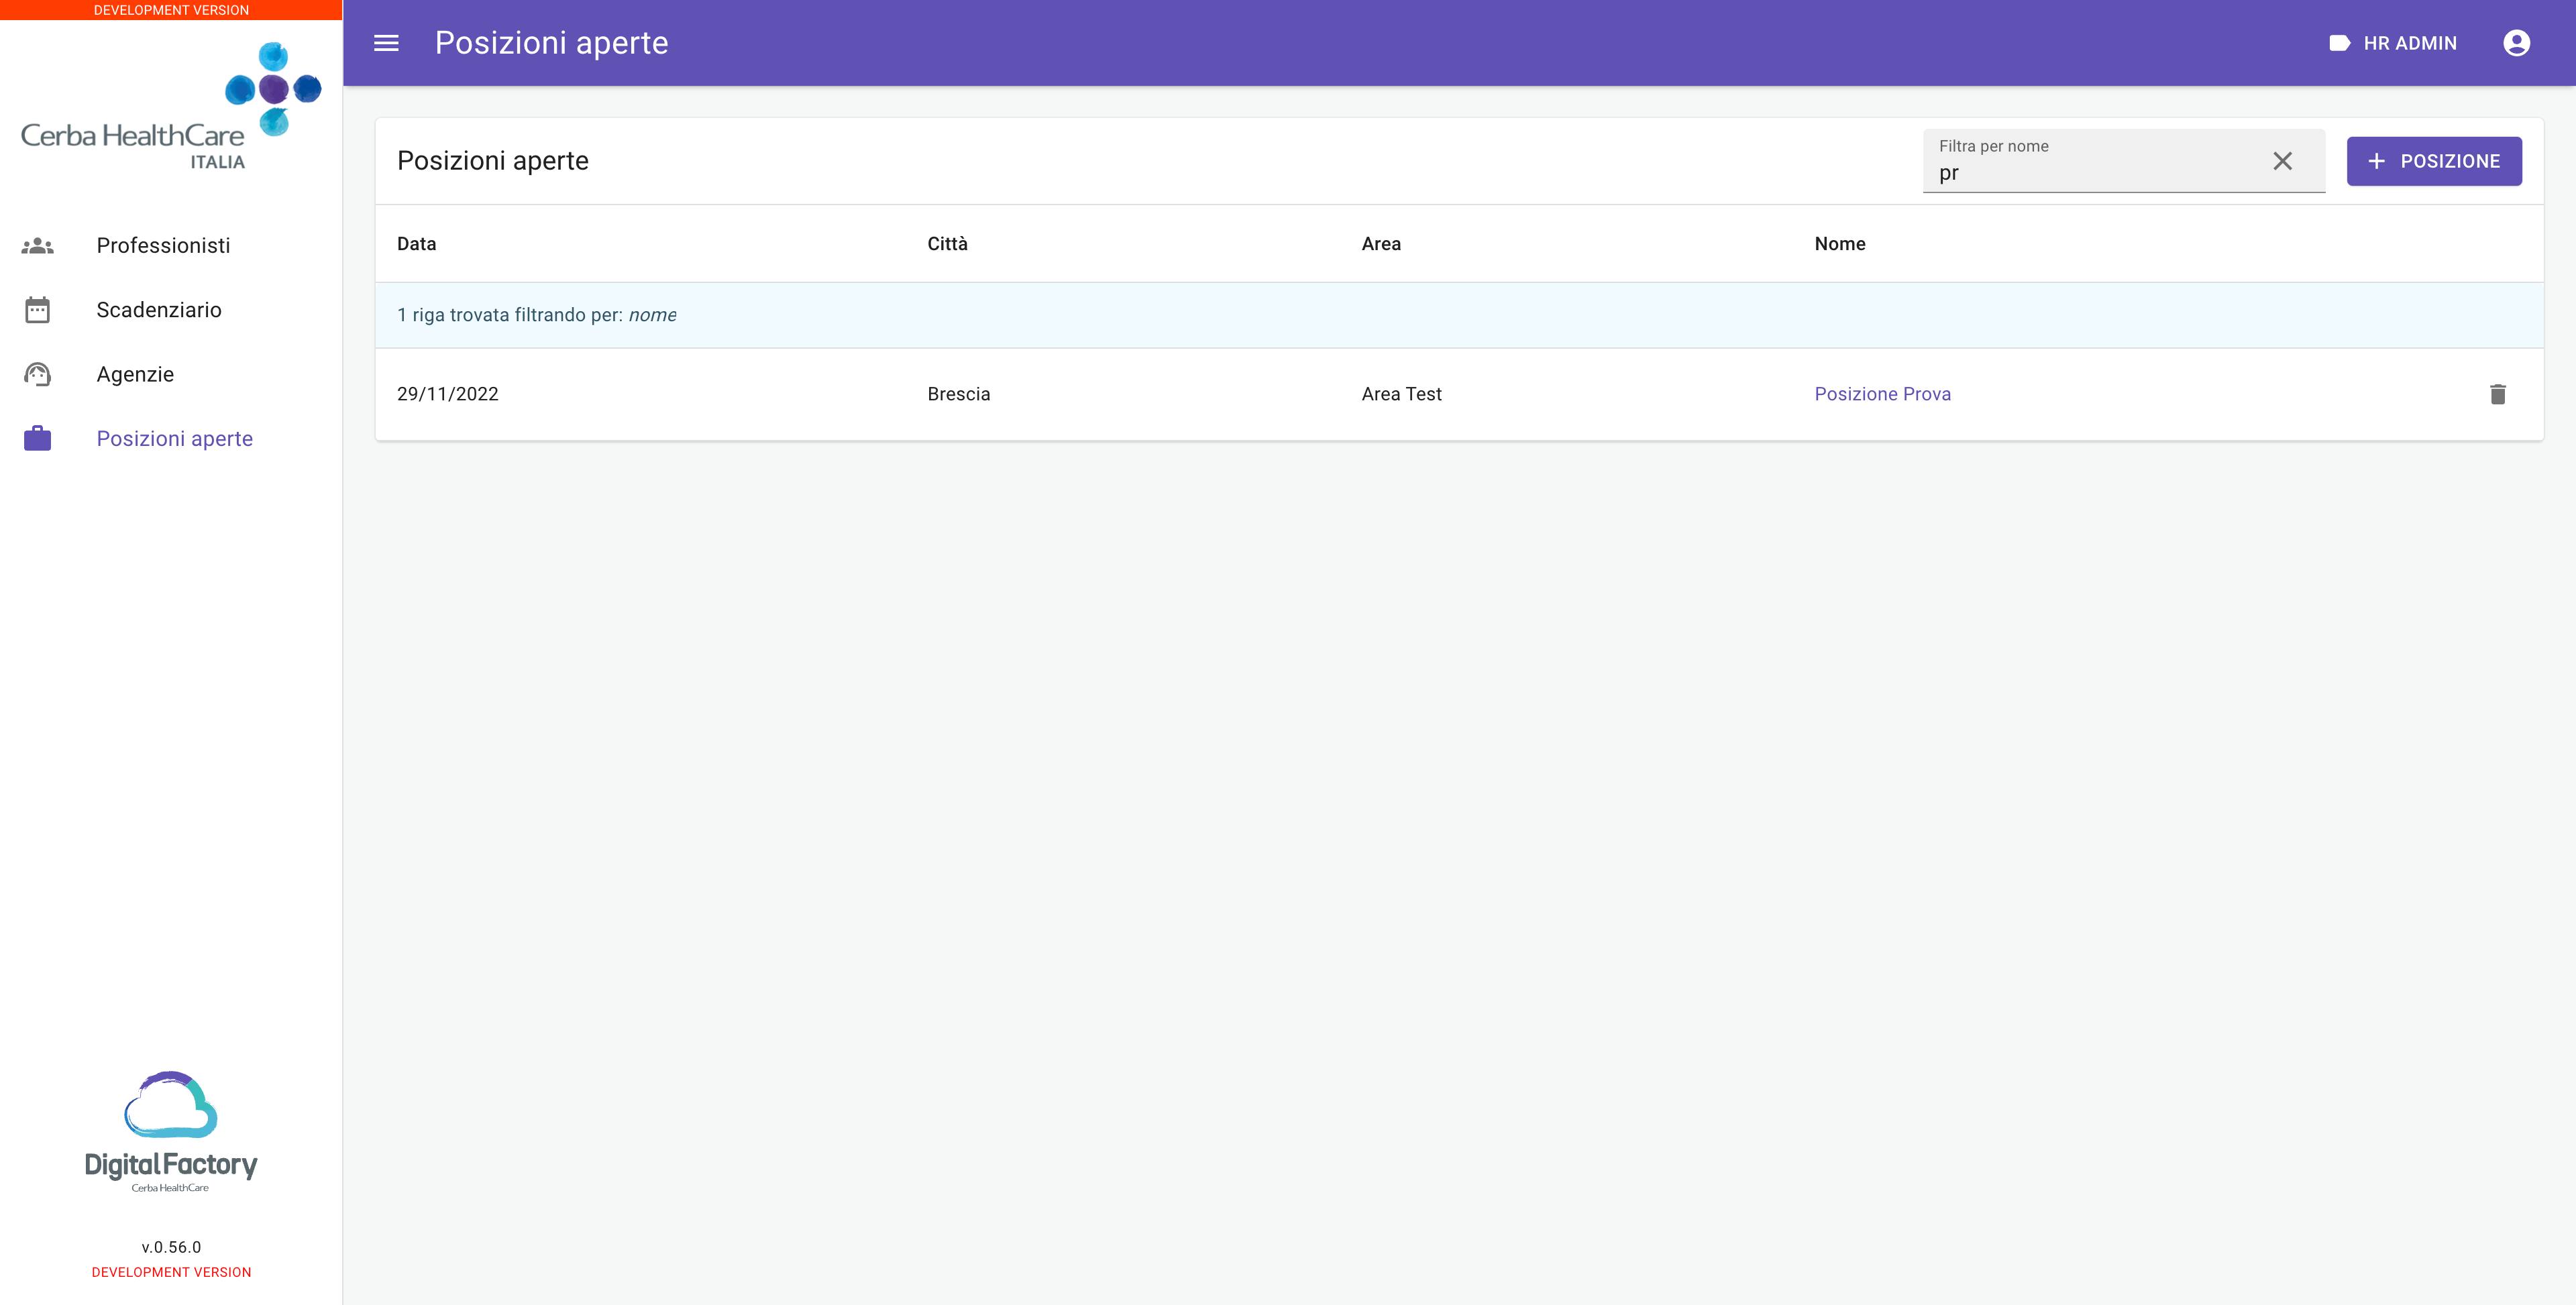
\includegraphics[width=0.75\textwidth]{images/capitolo5/f10_jobOpenPositions/PageJobOpenPositions_searchFilled.png} 
    \caption{Tabella posizioni aperte campo ricerca riempito} 
    \label{fig:PageJobOpenPositions_searchFilled}
\end{figure}

\begin{figure}[H]
    \centering
    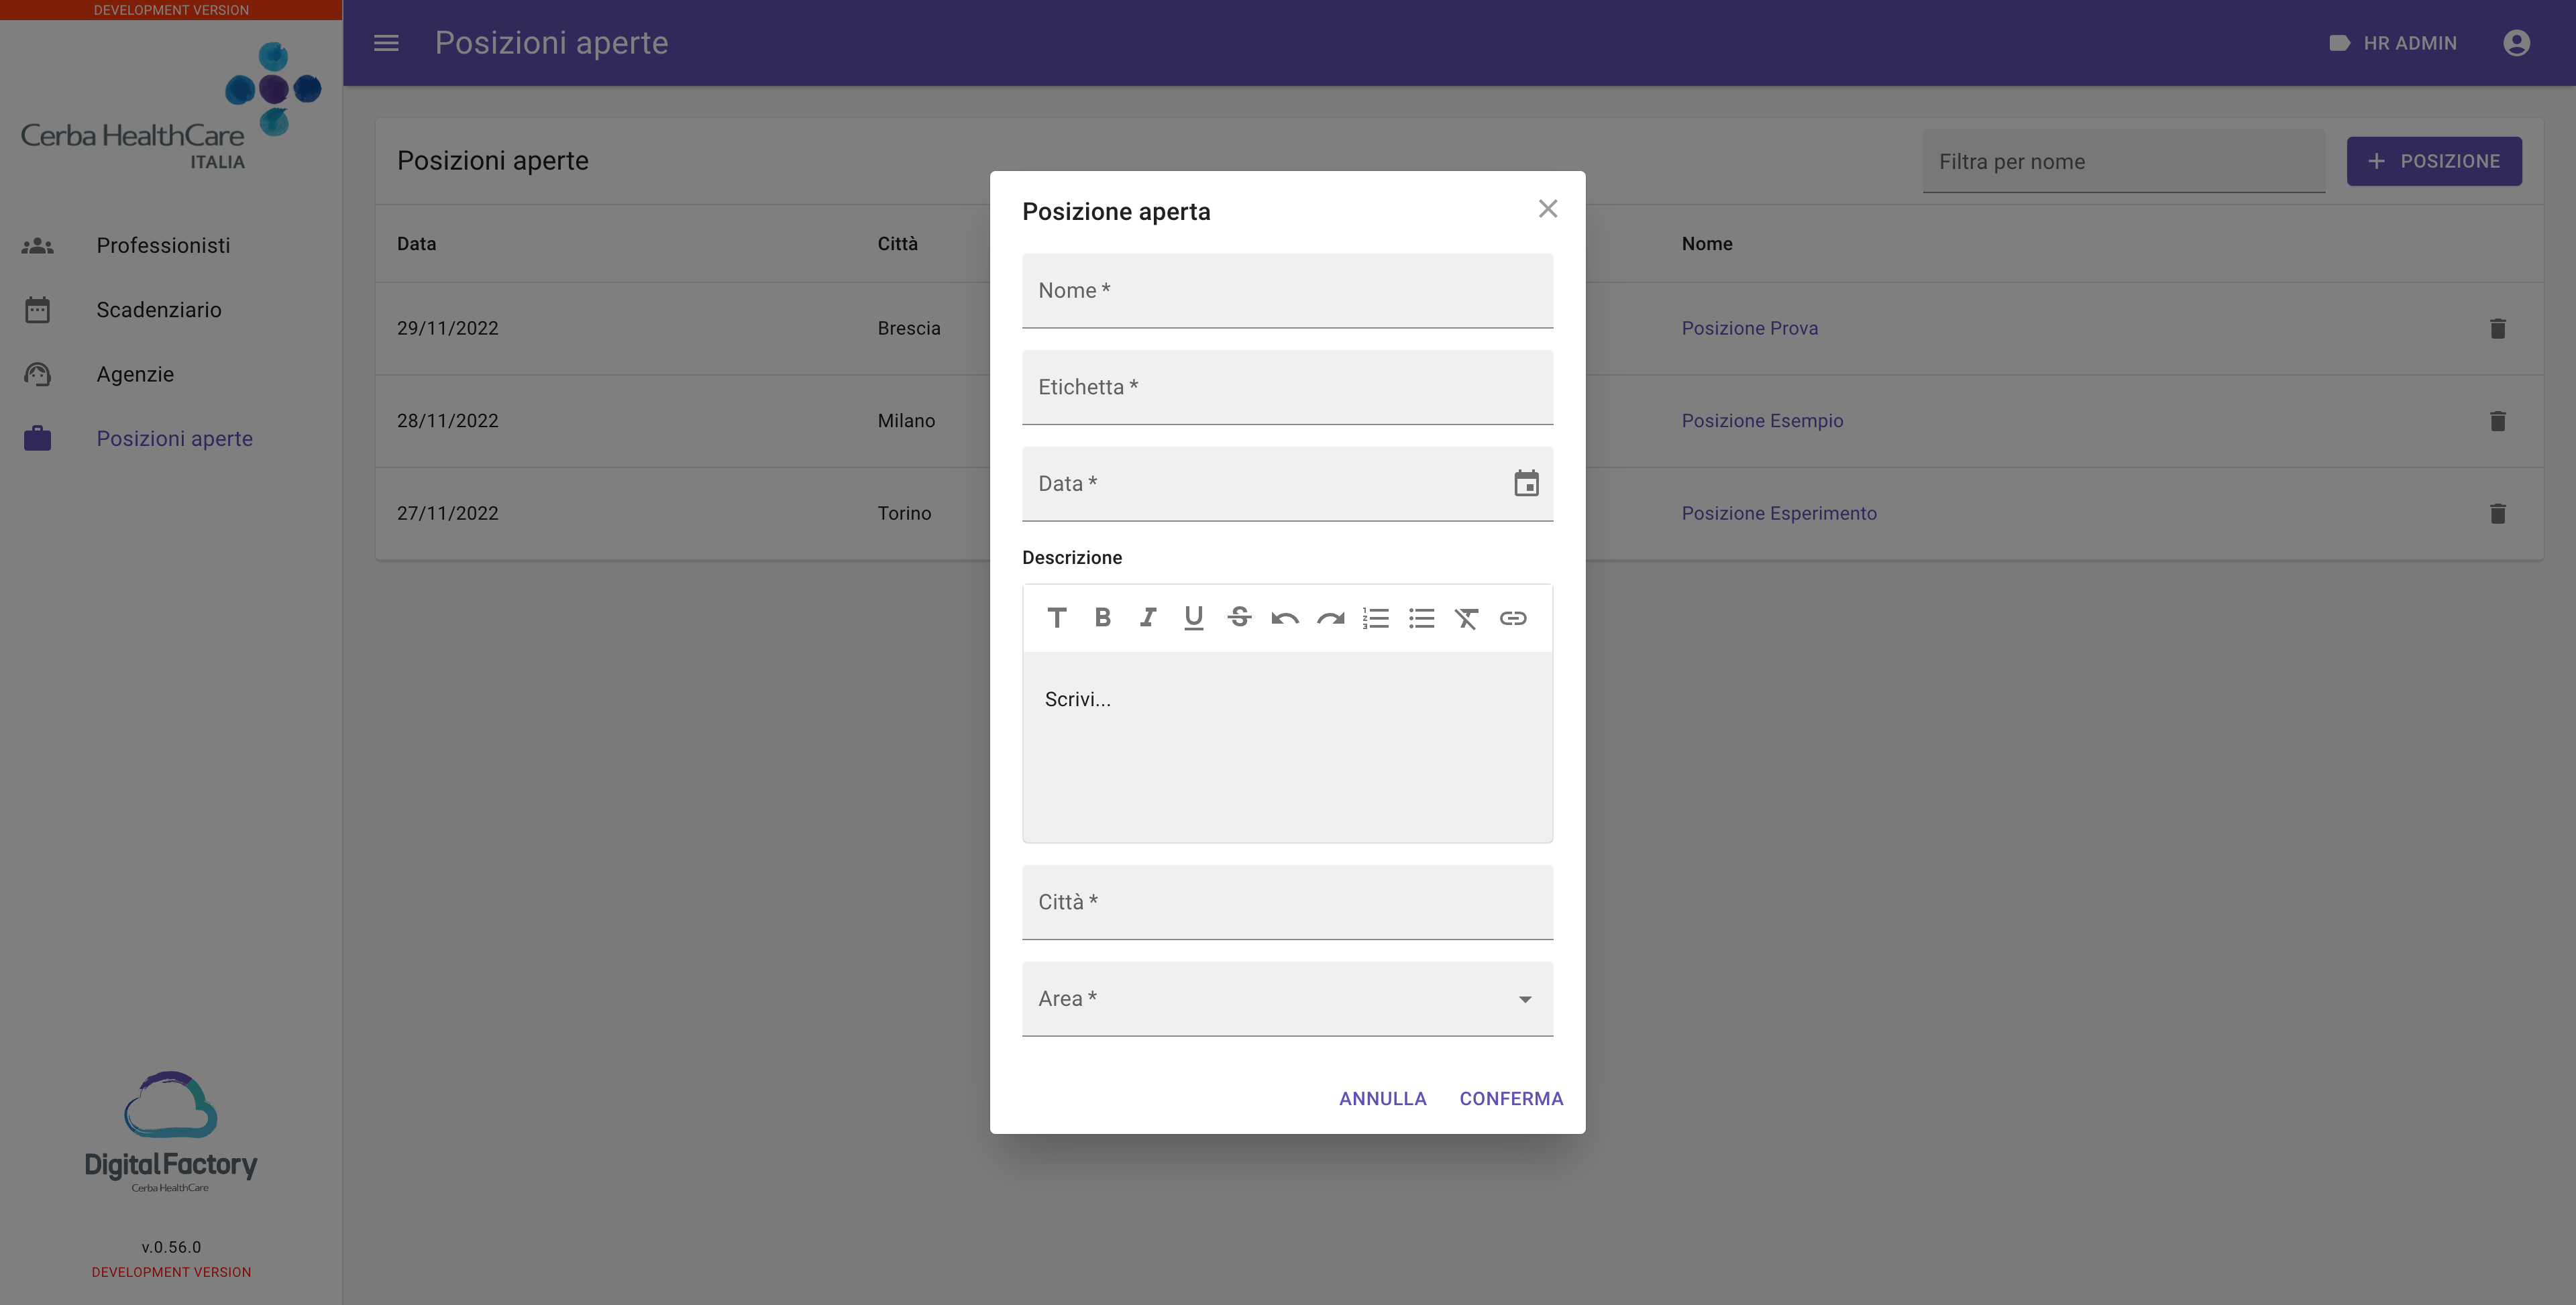
\includegraphics[width=0.75\textwidth]{images/capitolo5/f10_jobOpenPositions/ModalJobOpenPosition_create.png} 
    \caption{Modale aggiunta posizione aperta} 
    \label{fig:ModalJobOpenPosition_create}
\end{figure}

\begin{figure}[H]
    \centering
    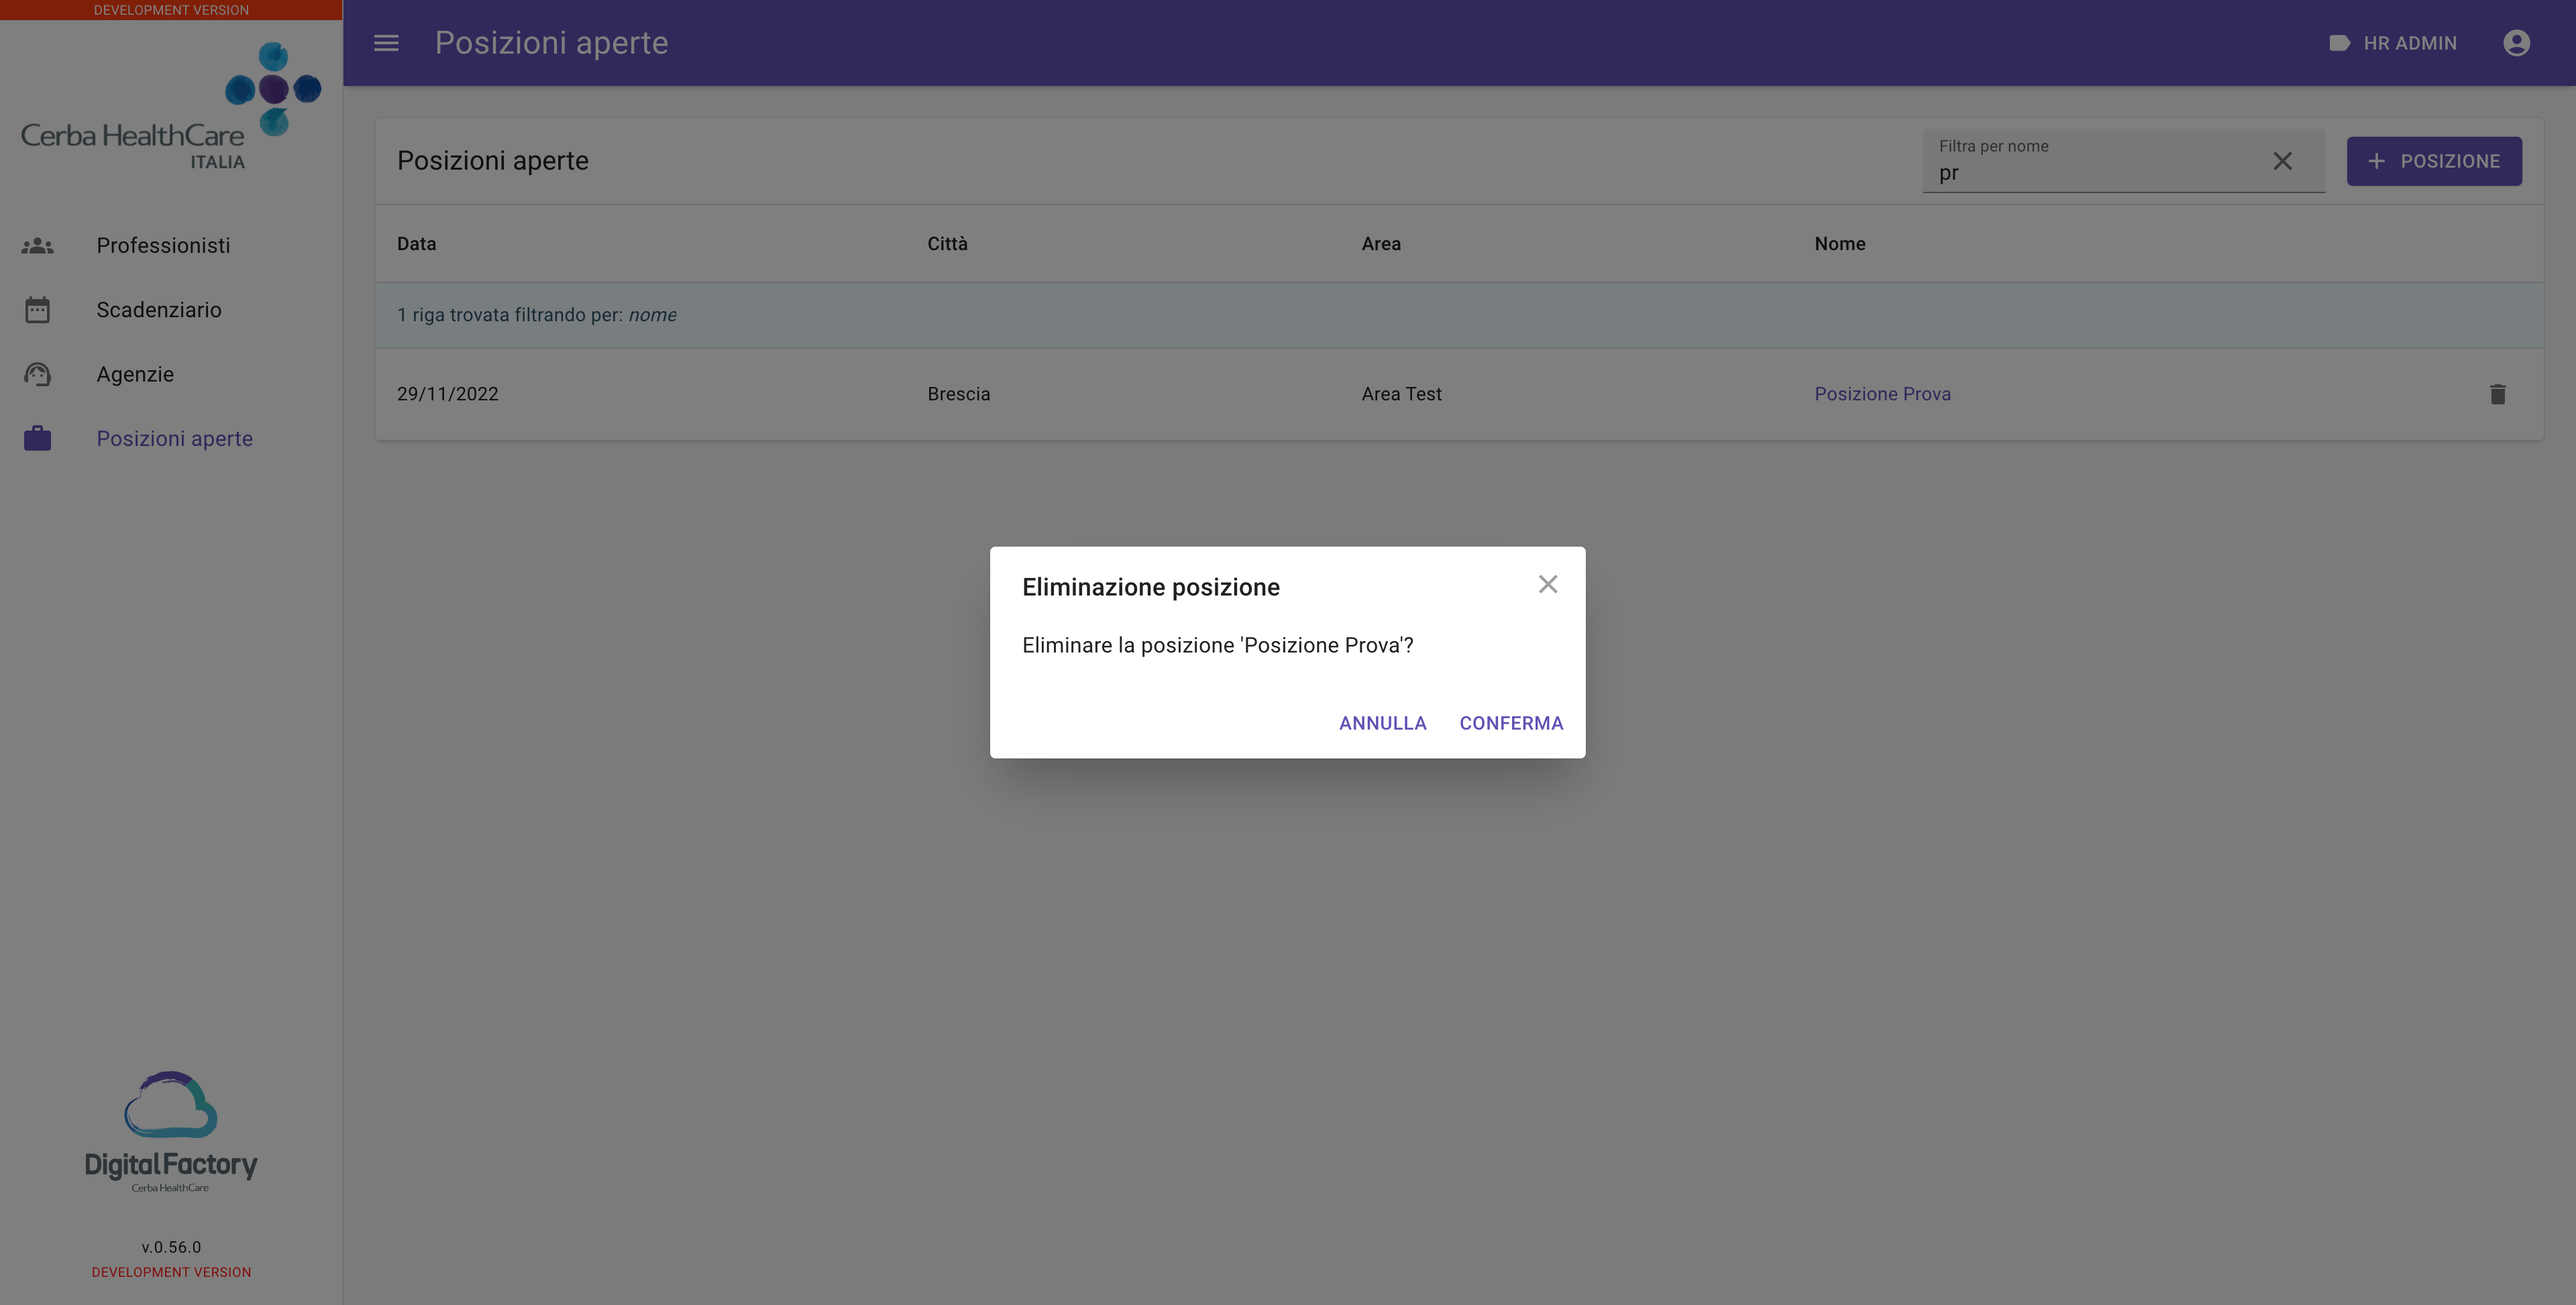
\includegraphics[width=0.75\textwidth]{images/capitolo5/f10_jobOpenPositions/ModalJobOpenPosition_delete.png} 
    \caption{Modale eliminazione posizione aperta} 
    \label{fig:ModalJobOpenPosition_delete}
\end{figure}

\begin{figure}[H]
    \centering
    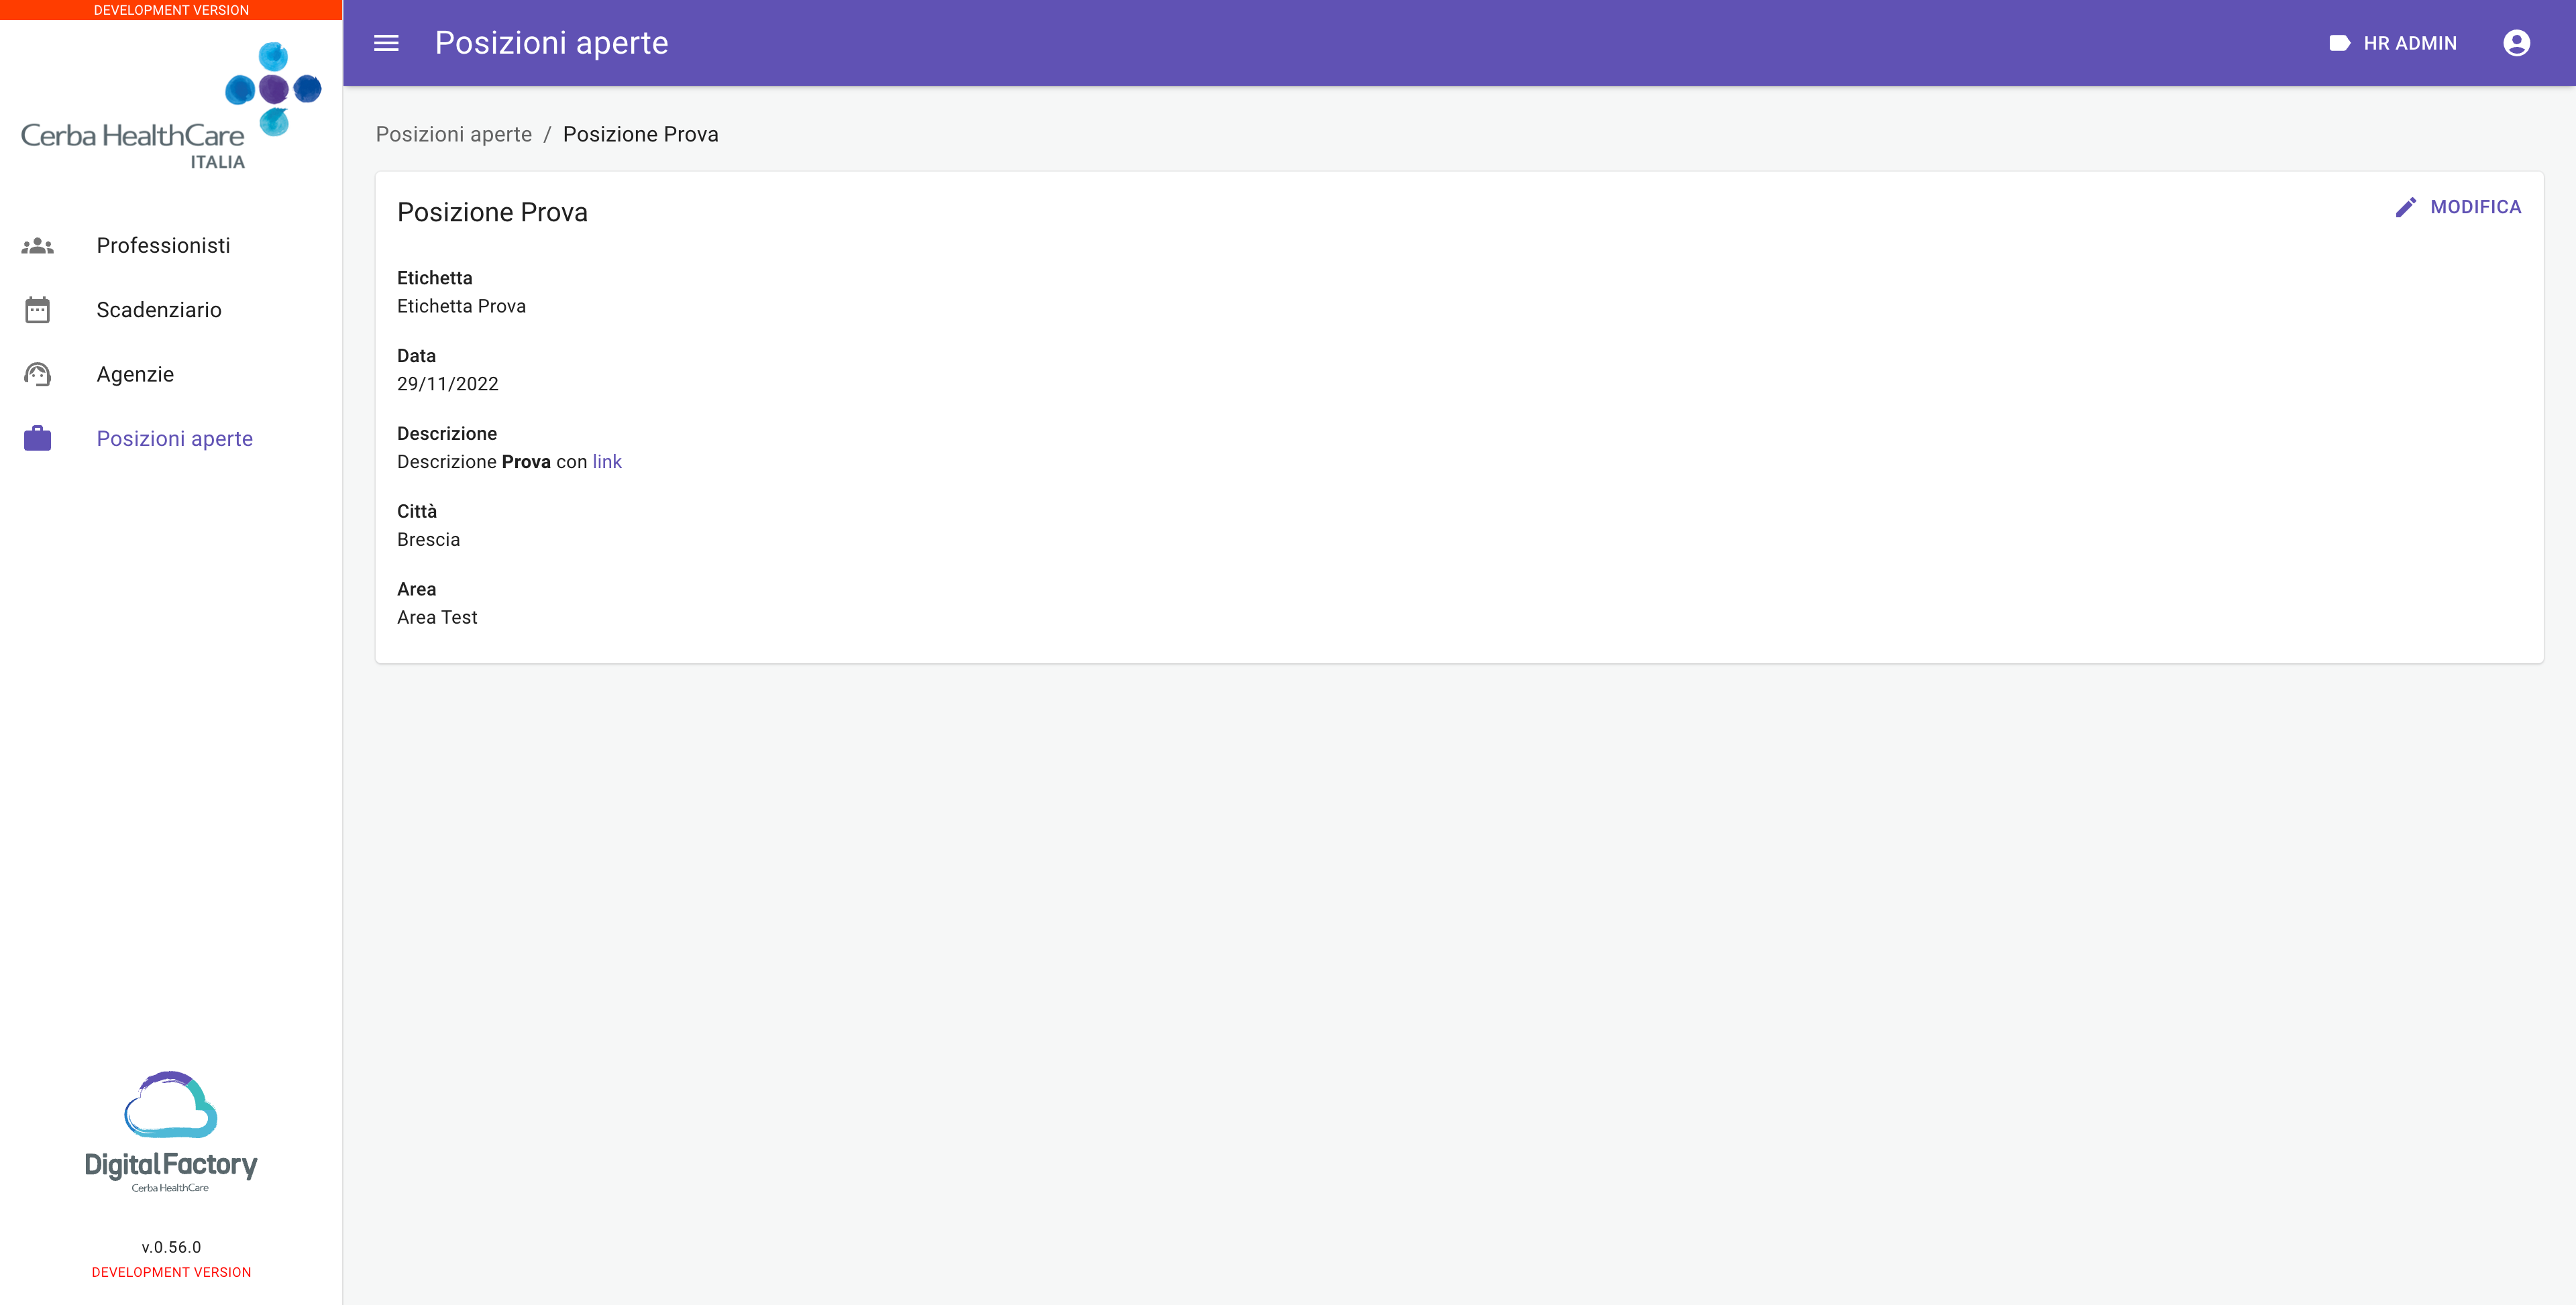
\includegraphics[width=0.75\textwidth]{images/capitolo5/f10_jobOpenPositions/PageJobOpenPosition.png} 
    \caption{Pagina dettaglio posizione aperta} 
    \label{fig:PageJobOpenPosition}
\end{figure}

\begin{figure}[H]
    \centering
    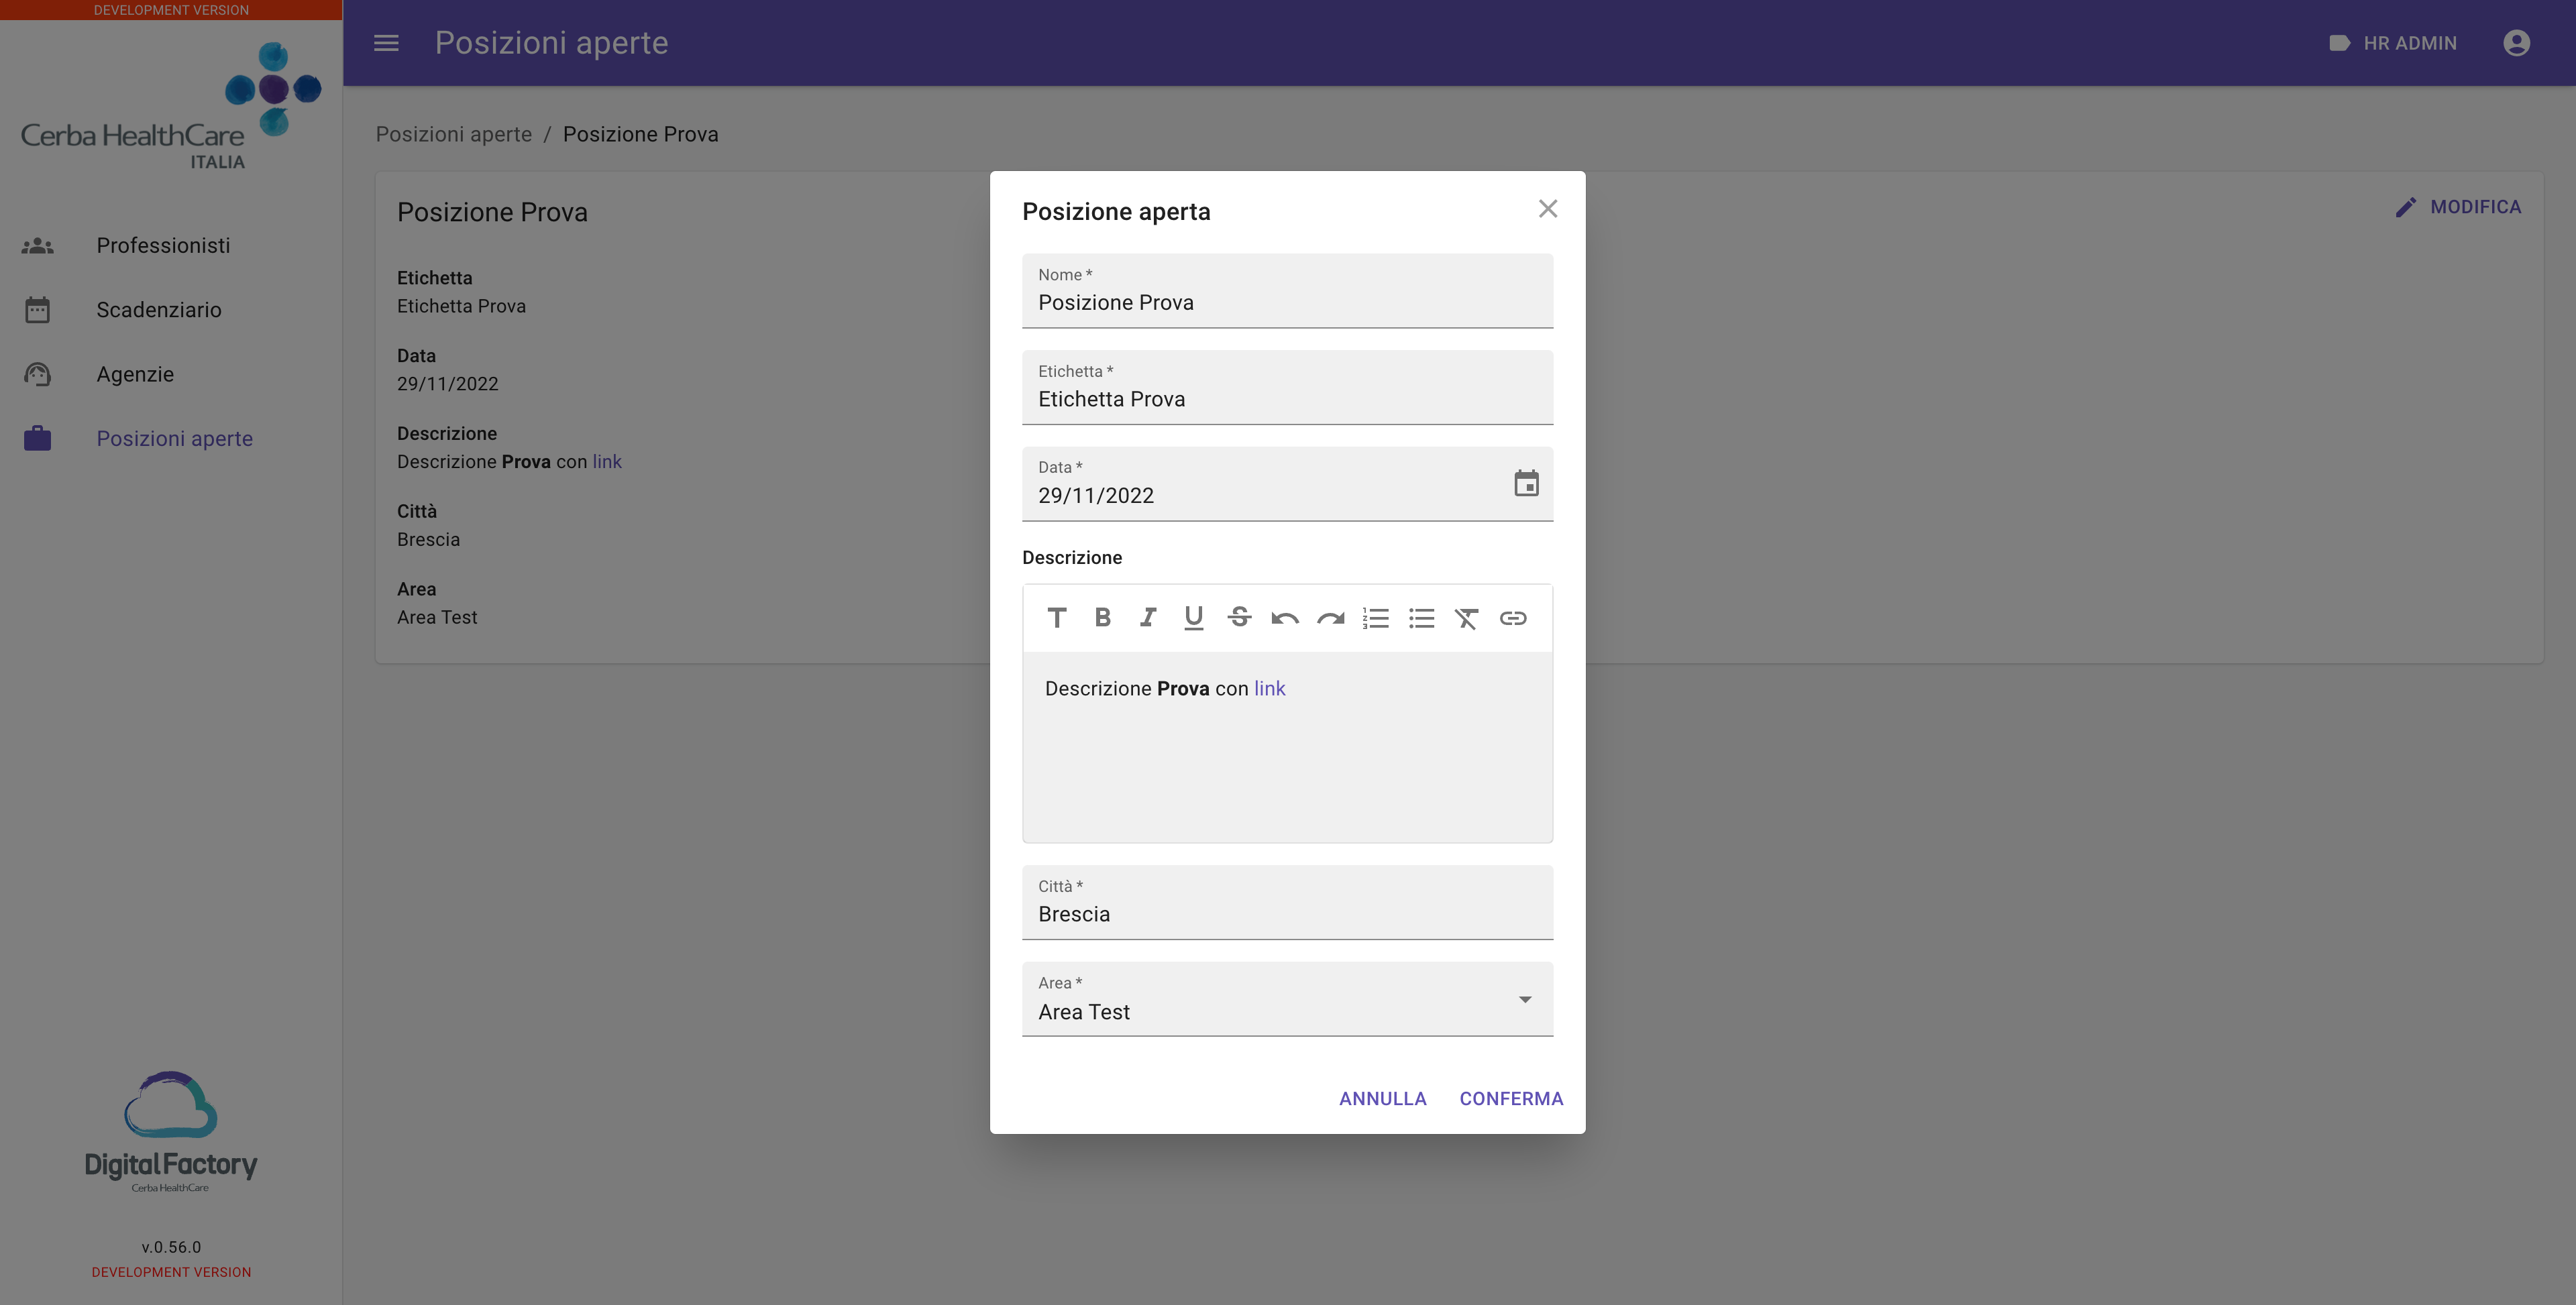
\includegraphics[width=0.75\textwidth]{images/capitolo5/f10_jobOpenPositions/ModalJobOpenPosition_edit.png} 
    \caption{Modale modifica posizione aperta} 
    \label{fig:ModalJobOpenPosition_edit}
\end{figure}

% \newpage\section{Bug}
% \label{sec:Bug}

% \subsection{B1: child}
